% !TEX root = thesis.tex
\chapter{Empirical Evaluation}
\label{chap:experiment}
In this chapter we evaluate our approach from Chapter~\ref{chap:approach}. We describe how we setup and conduct our empirical evaluation in Section~\ref{sec:experiment_setup} and we describe our experimental method in Section~\ref{sec:experiment_method}. Finally we discuss our experimental results in Section~\ref{sec:experiment_results} and threats to validity in Section~\ref{sec:experiment_threats}.


\section{Experimental Setup}
\label{sec:experiment_setup}
To encourage reproducibility of our empirical evaluation we discuss the specific details concerning environment (Section~\ref{subsec:experiment_environment}), tool configuration (Section~\ref{subsec:experiment_tool_configuration}), test subjects (Section~\ref{subsec:experiment_test_subjects}), and data preprocessing (Section~\ref{subsec:experiment_data_preprocessing}).


\subsection{Tool Configuration}
\label{subsec:experiment_tool_configuration}
We use three tools in our approach -- EMMA, Eclipse Metric Plugin and Javalanche. For all three tools, our approach manipulate the raw output of these tools to better support data synthesis. We use the default configuration for EMMA and the Eclipse Metric Plugin as these are already configured to provide the necessary data.

We configured Javalanche to better suite our approach. Although Javalanche has the ability to run parallel tasks, we did not utilize this feature. This was to avoid unnecessary issues that can occur due to concurrent access to file resources that a test suite may use. We enabled the coverage impact analysis of Javalanche as it provides comprehensive data regarding the mutants such as the type, location, and whether or not it was killed. The additional analysis is useful and required in the implementation of our approach, though it reduces the performance of Javalanche.

We perform 10-fold cross-validation as described in Section~\ref{sec:background_machine_learning}. LIBSVM provides an \emph{easy script} that automatically scales the data and makes parameter selection using a grid search~\cite{HCL03}. A grid search iterates over a range of parameters while measuring the effect it has on the classifiers performance. Parameter selection is a critical aspect of machine learning algorithms, and it can greatly influence the classification accuracy. We allow LIBSVM to automatically take care of this to best select the parameters based on the provided data. We allow LIBSVM to use eight threads for computation tasks. We also utilize the \gls{rbf} kernel as it is the default and comes recommended by the authors~\cite{HCL03}.

\subsection{Test Subjects}
\label{subsec:experiment_test_subjects}
We constructed three simple criteria to select our test subjects:

\begin{itemize}
  \item We selected software system that have a minimum of 5000 total \gls{sloc}. We decided to use this size as our minimum to avoid selecting \emph{toy} software systems that are not similar to \emph{real} software systems. Also, by using \emph{real} software systems we can potentially collect more data than that of \emph{toy} software systems.
  \item We selected open source projects as they are relatively easy to acquire as opposed to industry projects, and are freely available to analyze.
  \item Our approach required projects with a test suite or set of test cases as it is fundamentally required for mutation testing.
\end{itemize}

\begin{sidewaystable}[!tb]
  \centering
  \caption{The set of test subjects along with source code and test suite metrics.}
  \label{tab:experimental_subjects}
  \rowcolors{2}{gray!30}{gray!20}
  \begin{tabular}{|l|>{\raggedleft\arraybackslash}p{1.9cm}|>{\raggedleft\arraybackslash}p{1.9cm}|>{\raggedleft\arraybackslash}p{1.9cm}|>{\raggedleft\arraybackslash}p{1.9cm}|>{\raggedleft\arraybackslash}p{1.9cm}|>{\raggedleft\arraybackslash}p{1.9cm}|>{\raggedleft\arraybackslash}p{1.9cm}|}
    \hline
    \rowcolor[RGB]{169,196,223}
    \textbf{Program} & \textbf{Source LOC} & \textbf{Source Classes} & \textbf{Source Methods} & \textbf{Test LOC} & \textbf{Test Classes} & \textbf{Test Methods} & \textbf{Test Cases} \\
    \hline logback-core (1.0.3)~\cite{logback} & 12118 & 249 & 1270 & 8377 & 174 & 688 & 286 \\
    \hline barbecue (1.5-beta1)~\cite{barbecue} & 4790 & 58 & 299 & 2910 & 38 & 416 & 225 \\
    \hline jgap (3.6.1)~\cite{jgap} & 28975 & 415 & 3017 & 19694 & 180 & 1633 & 1355 \\
    \hline commons-lang (3.1)~\cite{commons-lang} & 19499 & 149 & 1196 & 33332 & 242 & 2408 & 2050 \\
    \hline joda-time (2.0)~\cite{joda-time} & 27139 & 227 & 3635 & 51388 & 221 & 4755 & 3866 \\
    \hline openfast (1.1.0)~\cite{openfast} & 11646 & 265 & 1447 & 5587 & 115 & 421 & 322 \\
    \hline jsoup (1.6.2)~\cite{jsoup} & 10949 & 198 & 954 & 2883 & 25 & 335 & 319 \\
    \hline joda-primitives (1.0)~\cite{joda-primitives} & 11157 & 128 & 1868 & 6989 & 49 & 746 & 1810 \\
    \hline \textbf{all} & \textbf{126273} & \textbf{1689} & \textbf{13686} & \textbf{131160} & \textbf{1044} & \textbf{11402} & \textbf{10233} \\
    \hline
  \end{tabular}
\end{sidewaystable}
\afterpage\clearpage

Following the criteria outlined, we selected the following eight open source Java projects shown in Table~\ref{tab:experimental_subjects}. A brief description of each open source software system used in our empirical evaluation is presented as follows:

\begin{itemize}
  \item \textbf{logback-core}: \emph{``Logback is intended as a successor to the popular log4j project, picking up where log4j leaves off. The logback-core module lays the groundwork for the other two modules''}~\cite{logback}.
  \item \textbf{barbecue}: \emph{``Barbecue is an open source, Java library that provides the means to create barcodes for printing and display in Java applications''}~\cite{barbecue}.
  \item \textbf{jgap}: \emph{``JGAP is a Genetic Algorithms and Genetic Programming component provided as a Java framework''}~\cite{jgap}.
  \item \textbf{commons-lang}: \emph{``The standard Java libraries fail to provide enough methods for manipulation of its core classes. Apache Commons Lang provides these extra methods''}\cite{commons-lang}.
  \item \textbf{joda-time}: \emph{``Joda-Time provides a quality replacement for the Java date and time classes. The design allows for multiple calendar systems, while still providing a simple API''}~\cite{joda-time}.
  \item \textbf{openfast}: \emph{``OpenFAST is a 100\% Java implementation of the FAST Protocol (FIX Adapted for STreaming). The FAST protocol is used to optimize communications in the electronic exchange of financial data''}~\cite{openfast}.
  \item \textbf{jsoup}: \emph{``jsoup is a Java library for working with real-world HTML. It provides a very convenient API for extracting and manipulating data, using the best of DOM, CSS, and jquery-like methods''}~\cite{jsoup}.
  \item \textbf{joda-primitives}: \emph{``Joda Primitives provides collections and utilities to bridge the gap between objects and primitive types in Java''}~\cite{joda-primitives}.
\end{itemize}

For our experiments we have eight test subjects that we can use individually, as well as consider them collectively. Therefore, we further refer to the collective set of all the individual test subjects as the \emph{all} set. By combining the individual test subjects we can evaluate our approach on a mixed set of data. Though each test subject is unique in terms of the functionality they provide and the specific structural design choices, each one is shares the commonality of being a software system. To further explore how our approach performs on different data, we consider eight additional sets using the \emph{all} set as the base, excluding an individual test subject. In other words we have 8 \emph{all\_but\_<subject>} sets, which is a combination of each individual test subject except the \emph{<subject>}. These additional sets allow us to evaluate our prediction approach by keeping one test subject completely isolated from the rest. As our approach focuses on prediction of mutation scores using metrics of the test subjects, the \emph{all} and \emph{all\_but\_<subject>} sets allow us to evaluate the generalizability of our approach on mixed and isolated test subjects.


\subsection{Data Preprocessing}
\label{subsec:experiment_data_preprocessing}
We first run each test subject through a verification \emph{test} that Javalanche provides. This test identifies any unit test cases that cannot execute properly or fail within Javalanche. We have to remove these test cases as the mutation testing process requires a test suite with no errors. We then import all the test subjects into Eclipse, as that is where the Eclipse Metrics Plugin operates. With our approach we simply configure our scripts to identify the test subject to collect data from, and the results are then stored in a database.


\subsection{Environment}
\label{subsec:experiment_environment}
We conducted all of the experiments for our empirical evaluation on a single machine that has six GB of \gls{ram}, a \gls{hdd} running at 7200 \gls{rpm}  and an Intel Core i7-870 processor running at 2.93 GHz. The environment is relevant as the mutation testing performance cost is dependant on the processor and \gls{hdd} speed.


\section{Experimental Method}
\label{sec:experiment_method}
Our empirical evaluation consists of five separate experiments:

\begin{itemize}
  \item \textbf{Mutation Score Distribution (Section~\ref{subsec:experiment_mutation_score_distribution})}: Using our test subjects described in Section~\ref{subsec:experiment_test_subjects}, we first want to understand their mutation testing results. Using our approach, we collect the source code, test suite metrics, and mutation scores of each test subject. As each test subject consists of multiple class- and method-level source code units, we are interested in the distribution of mutation scores. By understanding the distribution, we can gauge the available data that we will have for the later experiments and detect possible anomalies. We can also identify classification categories for the future experiments based on the mutation distribution as \gls{svm} have difficulty prediction real values (i.e., the mutation score).
  \item \textbf{Cross-Validation (Section~\ref{subsec:experiment_cross_validation})}: We identified features that describe source code units in Table~\ref{tab:metrics}. We grouped the features into sets (see Table~\ref{tab:feature_sets}) so we could evaluate how each set influences our classification performance. In this section we acquire the cross-validation accuracy for using the different feature sets over all the available data to identify the best feature set. We then evaluate the cross-validation accuracy over each individual test subject using the best set of features.
  \item \textbf{Prediction on Unknown Data(Section~\ref{subsec:experiment_prediction})}: Cross-validation accuracy provides a good indicator of classification performance, however it does not simulate realistic prediction on unknown data. In this section, we  control the training and testing data for our \gls{svm} to evaluate the prediction accuracy on unknown data. Using the \emph{all\_but\_<subject>} sets, we can evaluate the prediction accuracy when dealing with a unknown test subject that is isolated from the training data. We also evaluate the prediction accuracy of unknown data within an individual test subject. Both of these predictions are on unknown data but they explore the performance differences for prediction within a test subject, and against a different test subject.
  \item \textbf{Optimization and Generalization (Section~\ref{subsec:experiment_optimization_generalization})}: It is not known prior to predicting on unknown data what parameter values to use for the \gls{svm}. In Section~\ref{subsec:experiment_prediction}, the parameters are selected based on what maximizes the cross-validation accuracy with hopes that these parameters generalizes to the unknown data. In this section, we identify the most appropriate parameters that generalize to unknown data prediction. We evaluate the implications of using the generalizable parameters with respect to their impact on predicting unknown data.
  \item \textbf{Impact of Training Data Availability on Prediction Accuracy (Section~\ref{subsec:experiment_data})}: Using the findings from the previous experiments, we explore the impact of data availability on prediction accuracy. We graph the prediction accuracies against the amount of training data used for prediction. This experiment evaluates the applicability of using our approach in iterative development where it is beneficial to avoid evaluating every mutant generated.
\end{itemize}


\section{Experimental Results}
\label{sec:experiment_results}
The following five sections present experiments used in our empirical evaluation for our approach. Each section starts with a general research question that is addressed throughout the section.


\subsection{Mutation Score Distribution}
\label{subsec:experiment_mutation_score_distribution}
\begin{quote}
  \emph{\textbf{Research Question \#1:} What is the mutation score distribution of our test subjects?}
\end{quote}

\begin{quote}
  \emph{\textbf{Research Question \#2:} Using the distribution of our test subjects' mutation scores can we identify three categories of mutation scores to predict?}
\end{quote}

\begin{sidewaystable}[!tb]
  \centering
  \caption{Mutation testing results of the test subjects from Table~\ref{tab:experimental_subjects}.}
  \label{tab:experiments_mutation_results}
  \rowcolors{1}{gray!30}{gray!20}
  \begin{threeparttable}
    \begin{tabular}{|l|>{\raggedleft}p{2.5cm}|>{\raggedleft}p{2.5cm}|>{\raggedleft}p{2.5cm}|>{\raggedleft}p{2.5cm}|>{\raggedleft}p{2.5cm}|>{\raggedleft\arraybackslash}p{2.5cm}|}
      \rowcolor[RGB]{169,196,223}
      \hline & \textbf{Mutants Generated} & \textbf{Mutants Covered} & \textbf{Coverage Percent (\%)} & \textbf{Mutants Killed} & \textbf{Mutation Score (\%)\tnote{a}} & \textbf{Time Taken (\emph{hh:mm:ss})} \\
      \hline \cellcolor[RGB]{169,196,223} \textbf{logback-core} & 10682 & 7350 & 68.8073 & 5400 & 73.4694 & 01:49:10 \\
      \hline \cellcolor[RGB]{169,196,223} \textbf{barbecue} & 27324 & 4339 & 15.8798 & 2727 & 62.8486 & 00:49:51 \\
      \hline \cellcolor[RGB]{169,196,223} \textbf{jgap} & 31929 & 17903 & 56.0713 & 13328 & 74.4456 & 07:04:44 \\
      \hline \cellcolor[RGB]{169,196,223} \textbf{commons-lang} & 45141 & 41761 & 92.5124 & 33772 & 80.8697 & 15:51:59 \\
      \hline \cellcolor[RGB]{169,196,223} \textbf{joda-time} & 70594 & 58595 & 83.0028 & 48545 & 82.8484 & 31:55:50 \\
      \hline \cellcolor[RGB]{169,196,223} \textbf{openfast} & 14910 & 8371 & 56.1435 & 6869 & 82.0571 & 01:34:38 \\
      \hline \cellcolor[RGB]{169,196,223} \textbf{jsoup} & 14165 & 10540 & 74.4088 & 8430 & 79.9810 & 03:55:56 \\
      \hline \cellcolor[RGB]{169,196,223} \textbf{joda-primitives} & 22269 & 17334 & 77.8391 & 13499 & 77.8759 & 01:24:33 \\
      \hline \cellcolor[RGB]{169,196,223} \textbf{all} & \textbf{237014} & \textbf{166193} & \textbf{70.1195} & \textbf{132570} & \textbf{79.7687} & \textbf{64:26:41} \\
      \hline
    \end{tabular}
    \begin{tablenotes}
      \item[a] Mutation score is calculated using the covered and killed mutants.
    \end{tablenotes}
  \end{threeparttable}
  
  \vspace{3em}

  \centering
  \caption{The usable number of source code unit data points gathered from the test subjects in Table~\ref{tab:experimental_subjects}.}
  \label{tab:experiments_collected_data}
  \rowcolors{1}{gray!30}{gray!20}
  \begin{threeparttable}
    \begin{tabular}{|l|r|r|}
      \rowcolor[RGB]{169,196,223}
      \hline & \textbf{Class-Level} & \textbf{Method-Level} \\
      \hline \cellcolor[RGB]{169,196,223} \textbf{logback-core} & 115 & 447 \\
      \hline \cellcolor[RGB]{169,196,223} \textbf{barbecue} & 31 & 143 \\
      \hline \cellcolor[RGB]{169,196,223} \textbf{jgap} & 124 & 655 \\
      \hline \cellcolor[RGB]{169,196,223} \textbf{commons-lang} & 124 & 789 \\
      \hline \cellcolor[RGB]{169,196,223} \textbf{joda-time} & 194 & 2019 \\
      \hline \cellcolor[RGB]{169,196,223} \textbf{openfast} & 120 & 401 \\
      \hline \cellcolor[RGB]{169,196,223} \textbf{jsoup} & 83 & 381 \\
      \hline \cellcolor[RGB]{169,196,223} \textbf{joda-primitives} & 73 & 675 \\
      \hline \cellcolor[RGB]{169,196,223} \textbf{all} & \textbf{864} & \textbf{5510} \\
      \hline
    \end{tabular}
  \end{threeparttable}
\end{sidewaystable}
\afterpage\clearpage

\noindent
As described in Chapter~\ref{chap:approach}, our approach uses mutation testing to acquire the necessary mutation score data used for the category of the source code units. Table~\ref{tab:experiments_mutation_results} shows the results of running Javalanche on our test subjects. For all of our test subjects, mutation testing produced a large number of mutants that were evaluated, taking approximately 64 hours to complete in our experimental environment. As described in Section~\ref{subsec:background_mutation_tools}, Javalanche utilizes \emph{coverage} (i.e., basic block coverage) for test selection which limits the number of mutants to be evaluated to a subset of covered mutants. Javalanche was able to kill 79.7687\% of the covered mutants using all projects cumulatively. All individual projects, except for \emph{barbecue}, exceeded a mutation score of at least 73\% which indicates that the test suites for covered source code units are reasonably effective. The overall coverage is 70.1195\%, indicating that the test suites of the projects did not cover the reminding 29.8805\% of the generated mutants. Realistically, mutation scores are calculated using the entire project's source code, but for our purpose only covered mutants were used. The corrective action for non-covered mutants (i.e., mutants not covered by test suite using basic block coverage) is to add new test cases that provide coverage over the mutant's location.

\begin{figure}[!tb]
  \centering
  \begin{tikzpicture}
  \begin{axis}[
      bar width=1,
      ymajorgrids=true,
      xlabel=Mutation Score (\%),
      ylabel=\# of Classes,
      width=\linewidth,
      height=9.0cm]
      \addplot[ybar,fill=black] file {plots/all/evaluation_projects_class_distribution.txt};
  \end{axis}
  \end{tikzpicture}
  \caption{Mutation score distribution of classes from all eight test subjects from Table~\ref{tab:experimental_subjects} that can be used for training.}
  \vspace{2mm}
  \hrule
  \label{fig:mutation_distributions_class_all}
\end{figure}

\begin{figure}[!tb]
  \centering
  \begin{tikzpicture}
  \begin{axis}[
      bar width=1,
      ymajorgrids=true,
      xlabel=Mutation Score (\%),
      ylabel=\# of Methods,
      width=\linewidth,
      height=9.0cm]
      \addplot[ybar,fill=black] file {plots/all/evaluation_projects_method_distribution.txt};
  \end{axis}
  \end{tikzpicture}
  \caption{Mutation score distribution of methods from all eight test subjects from Table~\ref{tab:experimental_subjects} that can be used for training.}
  \vspace{2mm}
  \hrule
  \label{fig:mutation_distributions_method_all}
\end{figure}

\begin{figure}[!tb]
  \centering
  \begin{tikzpicture}
  \begin{axis}[
      xtick={0, 25, 50, 75, 100, 125, 150, 175, 200},
      xticklabels={0, 25, 50, 75, 100, 125, 150, 175, 200..6507},
      bar width=1,
      ymajorgrids=true,
      xlabel=\# of Covered Mutants,
      ylabel=\# of Classes,
      width=\linewidth,
      height=9.0cm]
      \addplot[ybar,fill=black] file {plots/all/covered_mutants_class_distribution.txt};
  \end{axis}
  \end{tikzpicture}
  \caption{Covered mutant distribution of classes from all eight test subjects from Table~\ref{tab:experimental_subjects} that can be used for training.}
  \vspace{1mm}
  \footnotesize{\emph{The above figure presents a subset of the full distribution by collapsing the values that exceed 200 into a single data point. The max number of covered mutants found was 6507, which corresponds to the following class \texttt{org.joda.time.format.ISODateTimeFormat} from the \texttt{joda-time} project.}}
  \vspace{2mm}
  \hrule
  \label{fig:covered_mutant_distributions_class_all}
\end{figure}

\begin{figure}[!tb]
  \centering
  \begin{tikzpicture}
  \begin{axis}[
      xtick={0, 25, 50, 75, 100, 125, 150, 175, 200},
      xticklabels={0, 25, 50, 75, 100, 125, 150, 175, 200..587},
      bar width=1,
      ymajorgrids=true,
      xlabel=\# of Covered Mutants,
      ylabel=\# of Methods,
      width=\linewidth,
      height=9.0cm]
      \addplot[ybar,fill=black] file {plots/all/covered_mutants_method_distribution.txt};
  \end{axis}
  \end{tikzpicture}
  \caption{Covered mutant distribution of methods from all eight test subjects from Table~\ref{tab:experimental_subjects} that can be used for training.}
  \vspace{1mm}
  \footnotesize{\emph{The above figure presents a subset of the full distribution by collapsing the values that exceed 200 into a single data point. There were 51 methods that had 117 covered mutants each, of these 48 are similar and are contained within the \texttt{ISODateTimeFormat} class of \texttt{joda-time}. The max number of covered mutants was 587, which corresponds to the \texttt{org.joda.time.format.PeriodFormatterBuilder\$FieldFormatter.parseInto} method.}}
  \vspace{2mm}
  \hrule
  \label{fig:covered_mutant_distributions_method_all}
\end{figure}

Source code and test code metrics were collected as described in Chapter~\ref{chap:approach}, which represented the set of feature data that make up the vectors of our \gls{svm}. Our approach can only make predictions using the synthesis of both mutation score data (i.e., category data) and source and test suite metrics (i.e., feature data) of source code units. If any piece of data is missing, we cannot use that source code unit for training and prediction purposes. Using our approach, we collected data for 864 class-level and 5510 method-level source code units (see Table~\ref{tab:experiments_collected_data}). We ignored abstract, anonymous, and overloaded source code units, because taking these into account would be a complex task. In addition to the ignored source code units we also ignored units with missing data (i.e., no tests cases), restricting the available data for further experiments. We present the distribution of the all the collected data points\footnote{\emph{Data points} are the \emph{vectors} or \emph{rows of data} within a \gls{svm} \emph{.libsvm} file.} for both class-level and method-level source code units with respect to mutation score in Figure~\ref{fig:mutation_distributions_class_all}~and~\ref{fig:mutation_distributions_method_all}. The mutation score distributions for each individual project are found in Appendix~\ref{app:mutation_score_distributions}. The mutation distribution of the both class- and method-level source code units are both negatively skewed, confirming our earlier observation that the test suite for the collected source code units are reasonably strong at detecting faults. We noticed that there were spikes comparative to their surroundings at the  0\%, 50\% and 100\% mutation score values, in particular the 100\% value is 2--9 times greater then other areas respectively. We speculate the spikes occur because a large number of source code units probably have small number of covered mutants (i.e., easier to kill all, evenly kill half or kill none). Analysis of the covered mutant distribution for class-level source code units (as seen in Figure~\ref{fig:covered_mutant_distributions_method_all}) shows a slightly denser grouping for low covered mutants. The positively skewed distribution of covered mutants for method-level source code units supports our speculation. With respect to the percentile of the class-level distribution of covered mutants, a quarter of the classes have less then 16 covered mutants. The method-level results show that half of the method have less then six covered mutants, and a quarter of the methods have less then two covered mutants. The distributions of covered mutants confirm our speculation that many of the source code units have a low number of covered mutants, which can contribute to the high 0\%, 50\% and 100\% mutation scores.

In Section~\ref{subsec:approach_create_libsvm_file}, we mentioned that our approached would create \emph{.libsvm} files using the acquire data. The category data required for the files that the \gls{svm} utilized based on the mutation score of source code units. To avoid predicting the exact mutation score (i.e., a set of real numbers), we instead used an abstracted set of categories (i.e., ranges of mutation scores). We were unsure how to properly select the ranges to use for our categories, but eventually decided to base our categories on the distribution of mutation scores from Figure~\ref{fig:covered_mutant_distributions_class_all}~and~\ref{fig:covered_mutant_distributions_method_all}. We found that the class-level distribution has a 25$^{th}$, 50$^{th}$ and 75$^{th}$ percentile of 72\%, 81\%, 89\% respectively, and for same percentiles of the method-level distribution are 75\%, 87\%, 99\%. Using these values we decided to use the following as our general case for categories:

\begin{itemize}
  \item \textbf{LOW} = [0\% -- 70\%)
  \item \textbf{MEDIUM} = [70\% -- 90\%)
  \item \textbf{HIGH} = [90\% -- 100\%]
\end{itemize}

The rational behind the categories is to separate the lower and upper percentiles in to the LOW and HIGH category, with the remaining into the MEDIUM category. We believe that these values will provide a sufficient level of information over the mutation testing coverage of the source code units.


\subsection{Cross-Validation}
\label{subsec:experiment_cross_validation}
\begin{quote}
  \emph{\textbf{Research Question:} Using the test suite and source code data from our test subjects can we identify a set of features that maximize cross-validation accuracy?}
\end{quote}

\begin{table}[!tb]
  \centering
  \rowcolors{2}{gray!30}{gray!20}
  \begin{tabular}{|l|>{\raggedleft\arraybackslash}p{3cm}|>{\raggedleft\arraybackslash}p{3cm}|>{\raggedleft\arraybackslash}p{3cm}|}
    \hline
    \rowcolor[RGB]{169,196,223}
    \textbf{Category} & \textbf{Mutation Score Range} & \textbf{Class-Level Units} & \textbf{Method-Level Units} \\
    \hline LOW & [0\% -- 70\%) & 191 & 1104 \\
    \hline MEDIUM & [70\% -- 90\%) & 459 & 1782 \\
    \hline HIGH & [90\% -- 100\%] & 214 & 2624 \\
    \hline
  \end{tabular}
  \caption{The available number of source code units that fall within the determined ranges of mutation scores.}
  \vspace{2mm}
  \hrule
  \label{tab:available_data}
\end{table}

\noindent
Using the determined classification categories from the previous section, we have imbalanced training data for class- and method-level source code units as shown in Table~\ref{tab:available_data}. Imbalanced data occurs when the data is not evenly distributed across the classification categories. This can be problematic for supervised machine learning techniques as they will heavily classify towards the majority category~\cite{BOSB10}. Barandela et al. indicate that there are three strategies to reduce the problem of imbalanced training data: Over-sample, under-sample, or internally bias the classification process~\cite{BVSF04}. It was shown that simple random under-sampling can be an effective solution (though not always the best) to this problem~\cite{Jap00,AKJ04}. As Akbani et al. mentioned \emph{``\ldots we are throwing away valid instances, which contain valuable information''}~\cite{AKJ04}, therefore we might be limiting the ability to generalize to new unknown data. The alternative is to perform over-sampling, as Batista et al. mention \emph{``\ldots random over-sampling can increase the likelihood of occurring overfitting, since it makes exact copies of the minority class examples''}~\cite{BPM04}. We decided to utilize random under-sampling as it provides a simple approach to dealing with imbalanced data. Furthermore the imbalanced data is not too severe (having a ratio of approximately 2:5), thus we believe we are not losing that much information by under-sampling our training data.

\begin{figure}[!tb]
  \centering
  \begin{adjustbox}{max size={.95\textwidth}{.95\textheight}}
    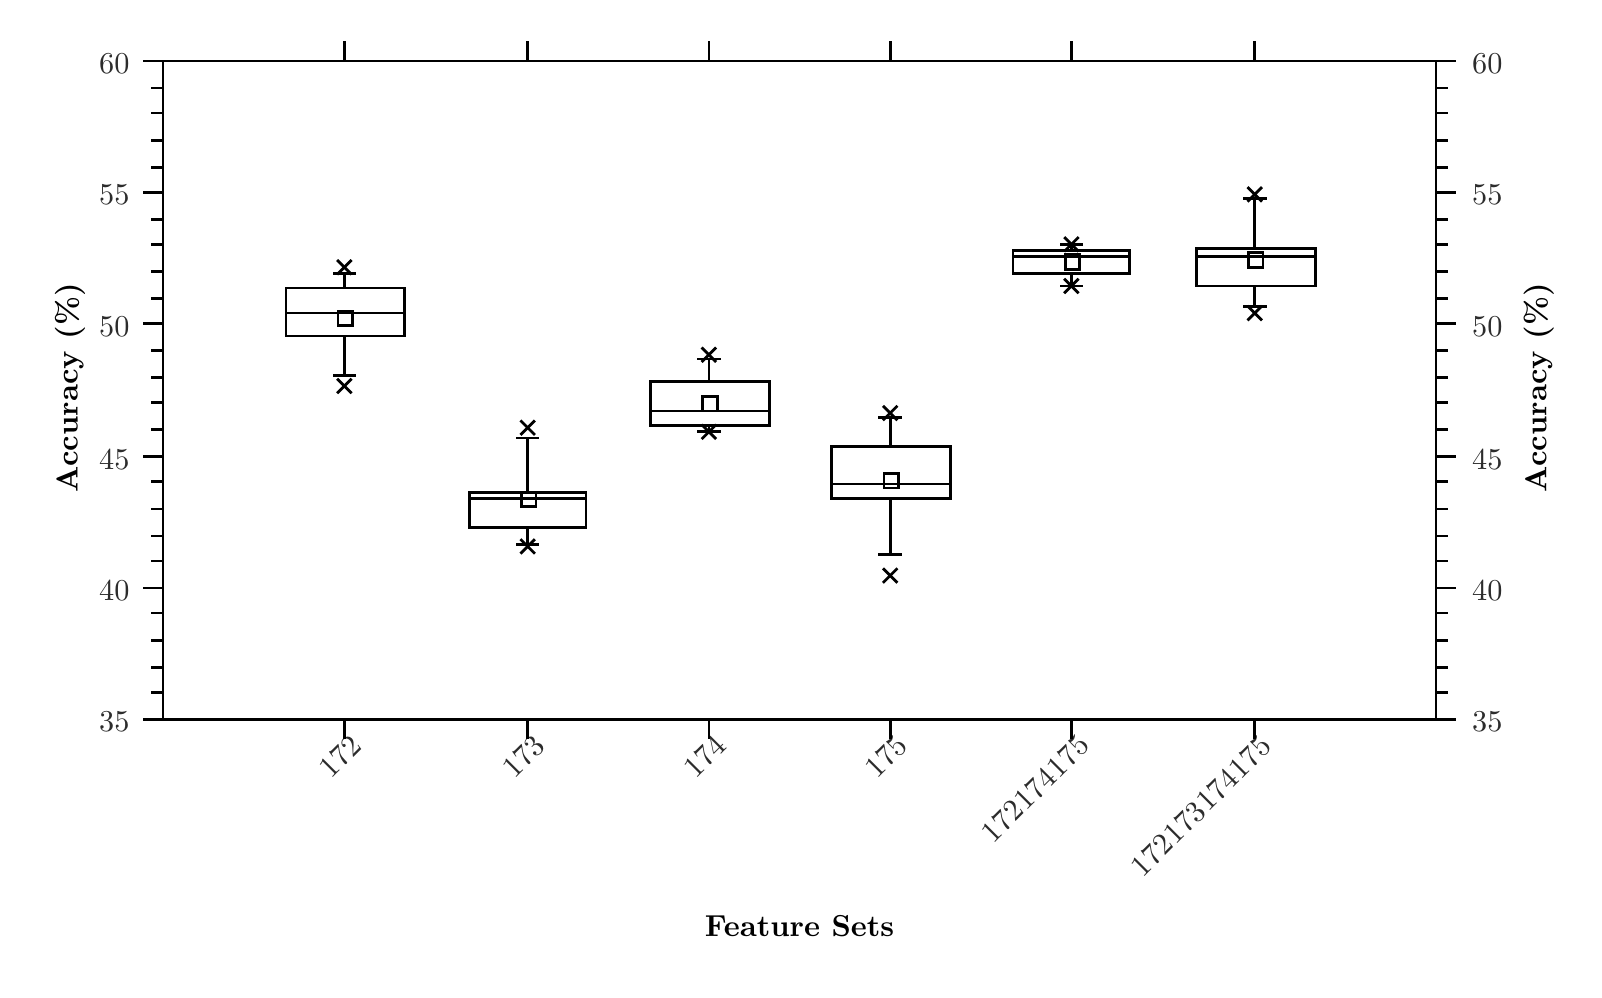
\begin{tikzpicture}{0pt}{0pt}{742pt}{452pt}
	\clip(0pt,452pt) -- (558.587pt,452pt) -- (558.587pt,111.729pt) -- (0pt,111.729pt) -- (0pt,452pt);
\begin{scope}
	\clip(48.9328pt,439.955pt) -- (508.901pt,439.955pt) -- (508.901pt,202.066pt) -- (48.9328pt,202.066pt) -- (48.9328pt,439.955pt);
	\color[rgb]{0,0,0}
	\draw[line width=1pt, line join=miter, line cap=rect](93.3487pt,357.898pt) -- (136.259pt,357.898pt) -- (136.259pt,340.584pt) -- (93.3487pt,340.584pt) -- (93.3487pt,357.898pt);
	\color[rgb]{0,0,0}
	\draw[line width=1pt, line join=miter, line cap=rect](110.663pt,326.28pt) -- (118.192pt,326.28pt);
	\draw[line width=1pt, line join=miter, line cap=rect](110.663pt,363.168pt) -- (118.192pt,363.168pt);
	\draw[line width=1pt, line join=miter, line cap=rect](114.427pt,363.168pt) -- (114.427pt,357.898pt);
	\draw[line width=1pt, line join=miter, line cap=rect](114.427pt,326.28pt) -- (114.427pt,340.584pt);
	\draw[line width=1pt, line join=miter, line cap=rect](93.3487pt,348.865pt) -- (135.506pt,348.865pt);
	\draw[line width=1pt, line join=miter, line cap=rect](112.169pt,324.775pt) -- (116.686pt,320.258pt);
	\draw[line width=1pt, line join=miter, line cap=rect](112.169pt,320.258pt) -- (116.686pt,324.775pt);
	\draw[line width=1pt, line join=miter, line cap=rect](112.169pt,367.685pt) -- (116.686pt,363.168pt);
	\draw[line width=1pt, line join=miter, line cap=rect](112.169pt,363.168pt) -- (116.686pt,367.685pt);
	\draw[line width=1pt, line join=miter, line cap=rect](112.169pt,349.618pt) -- (117.439pt,349.618pt) -- (117.439pt,344.348pt) -- (112.169pt,344.348pt) -- (112.169pt,349.618pt);
	\draw[line width=1pt, line join=miter, line cap=rect](159.596pt,284.123pt) -- (201.754pt,284.123pt) -- (201.754pt,271.325pt) -- (159.596pt,271.325pt) -- (159.596pt,284.123pt);
	\draw[line width=1pt, line join=miter, line cap=rect](176.911pt,265.303pt) -- (184.439pt,265.303pt);
	\draw[line width=1pt, line join=miter, line cap=rect](176.911pt,303.696pt) -- (184.439pt,303.696pt);
	\draw[line width=1pt, line join=miter, line cap=rect](180.675pt,303.696pt) -- (180.675pt,284.123pt);
	\draw[line width=1pt, line join=miter, line cap=rect](180.675pt,265.303pt) -- (180.675pt,271.325pt);
	\draw[line width=1pt, line join=miter, line cap=rect](159.596pt,281.864pt) -- (201.754pt,281.864pt);
	\draw[line width=1pt, line join=miter, line cap=rect](178.417pt,266.808pt) -- (182.933pt,262.291pt);
	\draw[line width=1pt, line join=miter, line cap=rect](178.417pt,262.291pt) -- (182.933pt,266.808pt);
	\draw[line width=1pt, line join=miter, line cap=rect](178.417pt,309.718pt) -- (182.933pt,305.202pt);
	\draw[line width=1pt, line join=miter, line cap=rect](178.417pt,305.202pt) -- (182.933pt,309.718pt);
	\draw[line width=1pt, line join=miter, line cap=rect](178.417pt,284.123pt) -- (183.686pt,284.123pt) -- (183.686pt,278.853pt) -- (178.417pt,278.853pt) -- (178.417pt,284.123pt);
	\draw[line width=1pt, line join=miter, line cap=rect](225.091pt,324.022pt) -- (268.001pt,324.022pt) -- (268.001pt,308.213pt) -- (225.091pt,308.213pt) -- (225.091pt,324.022pt);
	\draw[line width=1pt, line join=miter, line cap=rect](242.406pt,305.954pt) -- (249.934pt,305.954pt);
	\draw[line width=1pt, line join=miter, line cap=rect](242.406pt,332.303pt) -- (249.934pt,332.303pt);
	\draw[line width=1pt, line join=miter, line cap=rect](246.17pt,332.303pt) -- (246.17pt,324.022pt);
	\draw[line width=1pt, line join=miter, line cap=rect](246.17pt,305.954pt) -- (246.17pt,308.213pt);
	\draw[line width=1pt, line join=miter, line cap=rect](225.091pt,313.482pt) -- (267.248pt,313.482pt);
	\draw[line width=1pt, line join=miter, line cap=rect](243.911pt,308.213pt) -- (248.428pt,303.696pt);
	\draw[line width=1pt, line join=miter, line cap=rect](243.911pt,303.696pt) -- (248.428pt,308.213pt);
	\draw[line width=1pt, line join=miter, line cap=rect](243.911pt,336.067pt) -- (248.428pt,331.55pt);
	\draw[line width=1pt, line join=miter, line cap=rect](243.911pt,331.55pt) -- (248.428pt,336.067pt);
	\draw[line width=1pt, line join=miter, line cap=rect](243.911pt,318.752pt) -- (249.181pt,318.752pt) -- (249.181pt,313.482pt) -- (243.911pt,313.482pt) -- (243.911pt,318.752pt);
	\draw[line width=1pt, line join=miter, line cap=rect](290.586pt,300.685pt) -- (333.496pt,300.685pt) -- (333.496pt,281.864pt) -- (290.586pt,281.864pt) -- (290.586pt,300.685pt);
	\draw[line width=1pt, line join=miter, line cap=rect](307.9pt,261.538pt) -- (315.428pt,261.538pt);
	\draw[line width=1pt, line join=miter, line cap=rect](307.9pt,311.224pt) -- (315.428pt,311.224pt);
	\draw[line width=1pt, line join=miter, line cap=rect](311.664pt,311.224pt) -- (311.664pt,300.685pt);
	\draw[line width=1pt, line join=miter, line cap=rect](311.664pt,261.538pt) -- (311.664pt,281.864pt);
	\draw[line width=1pt, line join=miter, line cap=rect](290.586pt,287.134pt) -- (332.743pt,287.134pt);
	\draw[line width=1pt, line join=miter, line cap=rect](309.406pt,256.269pt) -- (313.923pt,251.752pt);
	\draw[line width=1pt, line join=miter, line cap=rect](309.406pt,251.752pt) -- (313.923pt,256.269pt);
	\draw[line width=1pt, line join=miter, line cap=rect](309.406pt,314.988pt) -- (313.923pt,310.471pt);
	\draw[line width=1pt, line join=miter, line cap=rect](309.406pt,310.471pt) -- (313.923pt,314.988pt);
	\draw[line width=1pt, line join=miter, line cap=rect](309.406pt,290.898pt) -- (314.676pt,290.898pt) -- (314.676pt,285.628pt) -- (309.406pt,285.628pt) -- (309.406pt,290.898pt);
	\draw[line width=1pt, line join=miter, line cap=rect](356.08pt,371.449pt) -- (398.238pt,371.449pt) -- (398.238pt,363.168pt) -- (356.08pt,363.168pt) -- (356.08pt,371.449pt);
	\draw[line width=1pt, line join=miter, line cap=rect](373.395pt,358.651pt) -- (380.923pt,358.651pt);
	\draw[line width=1pt, line join=miter, line cap=rect](373.395pt,373.707pt) -- (380.923pt,373.707pt);
	\draw[line width=1pt, line join=miter, line cap=rect](377.159pt,373.707pt) -- (377.159pt,371.449pt);
	\draw[line width=1pt, line join=miter, line cap=rect](377.159pt,358.651pt) -- (377.159pt,363.168pt);
	\draw[line width=1pt, line join=miter, line cap=rect](356.08pt,369.191pt) -- (398.238pt,369.191pt);
	\draw[line width=1pt, line join=miter, line cap=rect](374.901pt,360.91pt) -- (379.418pt,356.393pt);
	\draw[line width=1pt, line join=miter, line cap=rect](374.901pt,356.393pt) -- (379.418pt,360.91pt);
	\draw[line width=1pt, line join=miter, line cap=rect](374.901pt,375.966pt) -- (379.418pt,371.449pt);
	\draw[line width=1pt, line join=miter, line cap=rect](374.901pt,371.449pt) -- (379.418pt,375.966pt);
	\draw[line width=1pt, line join=miter, line cap=rect](374.901pt,369.943pt) -- (380.17pt,369.943pt) -- (380.17pt,364.674pt) -- (374.901pt,364.674pt) -- (374.901pt,369.943pt);
	\draw[line width=1pt, line join=miter, line cap=rect](422.328pt,372.202pt) -- (465.238pt,372.202pt) -- (465.238pt,358.651pt) -- (422.328pt,358.651pt) -- (422.328pt,372.202pt);
	\draw[line width=1pt, line join=miter, line cap=rect](439.642pt,351.123pt) -- (447.171pt,351.123pt);
	\draw[line width=1pt, line join=miter, line cap=rect](439.642pt,390.269pt) -- (447.171pt,390.269pt);
	\draw[line width=1pt, line join=miter, line cap=rect](443.407pt,390.269pt) -- (443.407pt,372.202pt);
	\draw[line width=1pt, line join=miter, line cap=rect](443.407pt,351.123pt) -- (443.407pt,358.651pt);
	\draw[line width=1pt, line join=miter, line cap=rect](422.328pt,369.191pt) -- (464.485pt,369.191pt);
	\draw[line width=1pt, line join=miter, line cap=rect](441.148pt,351.123pt) -- (445.665pt,346.606pt);
	\draw[line width=1pt, line join=miter, line cap=rect](441.148pt,346.606pt) -- (445.665pt,351.123pt);
	\draw[line width=1pt, line join=miter, line cap=rect](441.148pt,394.033pt) -- (445.665pt,389.517pt);
	\draw[line width=1pt, line join=miter, line cap=rect](441.148pt,389.517pt) -- (445.665pt,394.033pt);
	\draw[line width=1pt, line join=miter, line cap=rect](441.148pt,370.696pt) -- (446.418pt,370.696pt) -- (446.418pt,365.427pt) -- (441.148pt,365.427pt) -- (441.148pt,370.696pt);
\end{scope}
\begin{scope}
	\color[rgb]{0,0,0}
	\pgftext[center, base, at={\pgfpoint{18.0675pt}{321.763pt}},rotate=90]{\fontsize{11}{0}\selectfont{\textbf{Accuracy (\%)}}}
	\color[rgb]{0.172549,0.172549,0.172549}
	\pgftext[center, base, at={\pgfpoint{31.3358pt}{197.549pt}}]{\fontsize{11}{0}\selectfont{35}}
	\pgftext[center, base, at={\pgfpoint{31.3358pt}{244.977pt}}]{\fontsize{11}{0}\selectfont{40}}
	\pgftext[center, base, at={\pgfpoint{31.3358pt}{292.404pt}}]{\fontsize{11}{0}\selectfont{45}}
	\pgftext[center, base, at={\pgfpoint{31.3358pt}{340.584pt}}]{\fontsize{11}{0}\selectfont{50}}
	\pgftext[center, base, at={\pgfpoint{31.3358pt}{388.011pt}}]{\fontsize{11}{0}\selectfont{55}}
	\pgftext[center, base, at={\pgfpoint{31.3358pt}{435.438pt}}]{\fontsize{11}{0}\selectfont{60}}
	\color[rgb]{0,0,0}
	\draw[line width=1pt, line join=bevel, line cap=rect](48.9328pt,211.853pt) -- (45.1688pt,211.853pt);
	\draw[line width=1pt, line join=bevel, line cap=rect](48.9328pt,220.887pt) -- (45.1688pt,220.887pt);
	\draw[line width=1pt, line join=bevel, line cap=rect](48.9328pt,230.673pt) -- (45.1688pt,230.673pt);
	\draw[line width=1pt, line join=bevel, line cap=rect](48.9328pt,240.46pt) -- (45.1688pt,240.46pt);
	\draw[line width=1pt, line join=bevel, line cap=rect](48.9328pt,259.28pt) -- (45.1688pt,259.28pt);
	\draw[line width=1pt, line join=bevel, line cap=rect](48.9328pt,268.314pt) -- (45.1688pt,268.314pt);
	\draw[line width=1pt, line join=bevel, line cap=rect](48.9328pt,278.1pt) -- (45.1688pt,278.1pt);
	\draw[line width=1pt, line join=bevel, line cap=rect](48.9328pt,287.887pt) -- (45.1688pt,287.887pt);
	\draw[line width=1pt, line join=bevel, line cap=rect](48.9328pt,306.707pt) -- (45.1688pt,306.707pt);
	\draw[line width=1pt, line join=bevel, line cap=rect](48.9328pt,316.494pt) -- (45.1688pt,316.494pt);
	\draw[line width=1pt, line join=bevel, line cap=rect](48.9328pt,325.528pt) -- (45.1688pt,325.528pt);
	\draw[line width=1pt, line join=bevel, line cap=rect](48.9328pt,335.314pt) -- (45.1688pt,335.314pt);
	\draw[line width=1pt, line join=bevel, line cap=rect](48.9328pt,354.134pt) -- (45.1688pt,354.134pt);
	\draw[line width=1pt, line join=bevel, line cap=rect](48.9328pt,363.921pt) -- (45.1688pt,363.921pt);
	\draw[line width=1pt, line join=bevel, line cap=rect](48.9328pt,373.707pt) -- (45.1688pt,373.707pt);
	\draw[line width=1pt, line join=bevel, line cap=rect](48.9328pt,382.741pt) -- (45.1688pt,382.741pt);
	\draw[line width=1pt, line join=bevel, line cap=rect](48.9328pt,401.562pt) -- (45.1688pt,401.562pt);
	\draw[line width=1pt, line join=bevel, line cap=rect](48.9328pt,411.348pt) -- (45.1688pt,411.348pt);
	\draw[line width=1pt, line join=bevel, line cap=rect](48.9328pt,421.135pt) -- (45.1688pt,421.135pt);
	\draw[line width=1pt, line join=bevel, line cap=rect](48.9328pt,430.168pt) -- (45.1688pt,430.168pt);
	\draw[line width=1pt, line join=bevel, line cap=rect](48.9328pt,202.066pt) -- (42.1575pt,202.066pt);
	\draw[line width=1pt, line join=bevel, line cap=rect](48.9328pt,249.493pt) -- (42.1575pt,249.493pt);
	\draw[line width=1pt, line join=bevel, line cap=rect](48.9328pt,296.921pt) -- (42.1575pt,296.921pt);
	\draw[line width=1pt, line join=bevel, line cap=rect](48.9328pt,345.101pt) -- (42.1575pt,345.101pt);
	\draw[line width=1pt, line join=bevel, line cap=rect](48.9328pt,392.528pt) -- (42.1575pt,392.528pt);
	\draw[line width=1pt, line join=bevel, line cap=rect](48.9328pt,439.955pt) -- (42.1575pt,439.955pt);
	\draw[line width=1pt, line join=bevel, line cap=rect](48.9328pt,439.955pt) -- (48.9328pt,202.066pt);
	\pgftext[center, base, at={\pgfpoint{548.8pt}{321.763pt}},rotate=90]{\fontsize{11}{0}\selectfont{\textbf{Accuracy (\%)}}}
	\color[rgb]{0.172549,0.172549,0.172549}
	\pgftext[center, base, at={\pgfpoint{527.439pt}{197.549pt}}]{\fontsize{11}{0}\selectfont{35}}
	\pgftext[center, base, at={\pgfpoint{527.439pt}{244.977pt}}]{\fontsize{11}{0}\selectfont{40}}
	\pgftext[center, base, at={\pgfpoint{527.439pt}{292.404pt}}]{\fontsize{11}{0}\selectfont{45}}
	\pgftext[center, base, at={\pgfpoint{527.439pt}{340.584pt}}]{\fontsize{11}{0}\selectfont{50}}
	\pgftext[center, base, at={\pgfpoint{527.439pt}{388.011pt}}]{\fontsize{11}{0}\selectfont{55}}
	\pgftext[center, base, at={\pgfpoint{527.439pt}{435.438pt}}]{\fontsize{11}{0}\selectfont{60}}
	\color[rgb]{0,0,0}
	\draw[line width=1pt, line join=bevel, line cap=rect](508.901pt,211.853pt) -- (512.665pt,211.853pt);
	\draw[line width=1pt, line join=bevel, line cap=rect](508.901pt,220.887pt) -- (512.665pt,220.887pt);
	\draw[line width=1pt, line join=bevel, line cap=rect](508.901pt,230.673pt) -- (512.665pt,230.673pt);
	\draw[line width=1pt, line join=bevel, line cap=rect](508.901pt,240.46pt) -- (512.665pt,240.46pt);
	\draw[line width=1pt, line join=bevel, line cap=rect](508.901pt,259.28pt) -- (512.665pt,259.28pt);
	\draw[line width=1pt, line join=bevel, line cap=rect](508.901pt,268.314pt) -- (512.665pt,268.314pt);
	\draw[line width=1pt, line join=bevel, line cap=rect](508.901pt,278.1pt) -- (512.665pt,278.1pt);
	\draw[line width=1pt, line join=bevel, line cap=rect](508.901pt,287.887pt) -- (512.665pt,287.887pt);
	\draw[line width=1pt, line join=bevel, line cap=rect](508.901pt,306.707pt) -- (512.665pt,306.707pt);
	\draw[line width=1pt, line join=bevel, line cap=rect](508.901pt,316.494pt) -- (512.665pt,316.494pt);
	\draw[line width=1pt, line join=bevel, line cap=rect](508.901pt,325.528pt) -- (512.665pt,325.528pt);
	\draw[line width=1pt, line join=bevel, line cap=rect](508.901pt,335.314pt) -- (512.665pt,335.314pt);
	\draw[line width=1pt, line join=bevel, line cap=rect](508.901pt,354.134pt) -- (512.665pt,354.134pt);
	\draw[line width=1pt, line join=bevel, line cap=rect](508.901pt,363.921pt) -- (512.665pt,363.921pt);
	\draw[line width=1pt, line join=bevel, line cap=rect](508.901pt,373.707pt) -- (512.665pt,373.707pt);
	\draw[line width=1pt, line join=bevel, line cap=rect](508.901pt,382.741pt) -- (512.665pt,382.741pt);
	\draw[line width=1pt, line join=bevel, line cap=rect](508.901pt,401.562pt) -- (512.665pt,401.562pt);
	\draw[line width=1pt, line join=bevel, line cap=rect](508.901pt,411.348pt) -- (512.665pt,411.348pt);
	\draw[line width=1pt, line join=bevel, line cap=rect](508.901pt,421.135pt) -- (512.665pt,421.135pt);
	\draw[line width=1pt, line join=bevel, line cap=rect](508.901pt,430.168pt) -- (512.665pt,430.168pt);
	\draw[line width=1pt, line join=bevel, line cap=rect](508.901pt,202.066pt) -- (515.677pt,202.066pt);
	\draw[line width=1pt, line join=bevel, line cap=rect](508.901pt,249.493pt) -- (515.677pt,249.493pt);
	\draw[line width=1pt, line join=bevel, line cap=rect](508.901pt,296.921pt) -- (515.677pt,296.921pt);
	\draw[line width=1pt, line join=bevel, line cap=rect](508.901pt,345.101pt) -- (515.677pt,345.101pt);
	\draw[line width=1pt, line join=bevel, line cap=rect](508.901pt,392.528pt) -- (515.677pt,392.528pt);
	\draw[line width=1pt, line join=bevel, line cap=rect](508.901pt,439.955pt) -- (515.677pt,439.955pt);
	\draw[line width=1pt, line join=bevel, line cap=rect](508.901pt,439.955pt) -- (508.901pt,202.066pt);
	\pgftext[center, base, at={\pgfpoint{278.911pt}{123.774pt}}]{\fontsize{11}{0}\selectfont{\textbf{Feature Sets}}}
	\color[rgb]{0.172549,0.172549,0.172549}
	\pgftext[center, base, at={\pgfpoint{115.392pt}{186.104pt}},rotate=45]{\fontsize{11}{0}\selectfont{\ding{172}}}
	\pgftext[center, base, at={\pgfpoint{181.64pt}{186.104pt}},rotate=45]{\fontsize{11}{0}\selectfont{\ding{173}}}
	\pgftext[center, base, at={\pgfpoint{247.135pt}{186.104pt}},rotate=45]{\fontsize{11}{0}\selectfont{\ding{174}}}
	\pgftext[center, base, at={\pgfpoint{312.629pt}{186.104pt}},rotate=45]{\fontsize{11}{0}\selectfont{\ding{175}}}
	\pgftext[center, base, at={\pgfpoint{354.702pt}{162.682pt}},rotate=45]{\fontsize{11}{0}\selectfont{\ding{172}}}
	\pgftext[center, base, at={\pgfpoint{366.513pt}{174.493pt}},rotate=45]{\fontsize{11}{0}\selectfont{\ding{174}}}
	\pgftext[center, base, at={\pgfpoint{378.324pt}{186.303pt}},rotate=45]{\fontsize{11}{0}\selectfont{\ding{175}}}
	\pgftext[center, base, at={\pgfpoint{408.706pt}{150.439pt}},rotate=45]{\fontsize{11}{0}\selectfont{\ding{172}}}
	\pgftext[center, base, at={\pgfpoint{420.517pt}{162.249pt}},rotate=45]{\fontsize{11}{0}\selectfont{\ding{173}}}
	\pgftext[center, base, at={\pgfpoint{432.328pt}{174.06pt}},rotate=45]{\fontsize{11}{0}\selectfont{\ding{174}}}
	\pgftext[center, base, at={\pgfpoint{444.139pt}{185.871pt}},rotate=45]{\fontsize{11}{0}\selectfont{\ding{175}}}
	\color[rgb]{0,0,0}
	\draw[line width=1pt, line join=bevel, line cap=rect](114.427pt,202.066pt) -- (114.427pt,195.291pt);
	\draw[line width=1pt, line join=bevel, line cap=rect](180.675pt,202.066pt) -- (180.675pt,195.291pt);
	\draw[line width=1pt, line join=bevel, line cap=rect](246.17pt,202.066pt) -- (246.17pt,195.291pt);
	\draw[line width=1pt, line join=bevel, line cap=rect](311.664pt,202.066pt) -- (311.664pt,195.291pt);
	\draw[line width=1pt, line join=bevel, line cap=rect](377.159pt,202.066pt) -- (377.159pt,195.291pt);
	\draw[line width=1pt, line join=bevel, line cap=rect](443.407pt,202.066pt) -- (443.407pt,195.291pt);
	\draw[line width=1pt, line join=bevel, line cap=rect](48.9328pt,202.066pt) -- (508.901pt,202.066pt);
	\draw[line width=1pt, line join=bevel, line cap=rect](114.427pt,439.955pt) -- (114.427pt,446.73pt);
	\draw[line width=1pt, line join=bevel, line cap=rect](180.675pt,439.955pt) -- (180.675pt,446.73pt);
	\draw[line width=1pt, line join=bevel, line cap=rect](246.17pt,439.955pt) -- (246.17pt,446.73pt);
	\draw[line width=1pt, line join=bevel, line cap=rect](311.664pt,439.955pt) -- (311.664pt,446.73pt);
	\draw[line width=1pt, line join=bevel, line cap=rect](377.159pt,439.955pt) -- (377.159pt,446.73pt);
	\draw[line width=1pt, line join=bevel, line cap=rect](443.407pt,439.955pt) -- (443.407pt,446.73pt);
	\draw[line width=1pt, line join=bevel, line cap=rect](48.9328pt,439.955pt) -- (508.901pt,439.955pt);
\end{scope}
\end{tikzpicture}

  \end{adjustbox}
  \caption{Class-level cross-validation accuracy of feature sets on the \emph{all} subject.}
  \vspace{2mm}
  \hrule
  \label{fig:all_cross_validation_features_class_graph}
\end{figure}

\begin{figure}[!tb]
  \centering
  \begin{adjustbox}{max size={.95\textwidth}{.95\textheight}}
    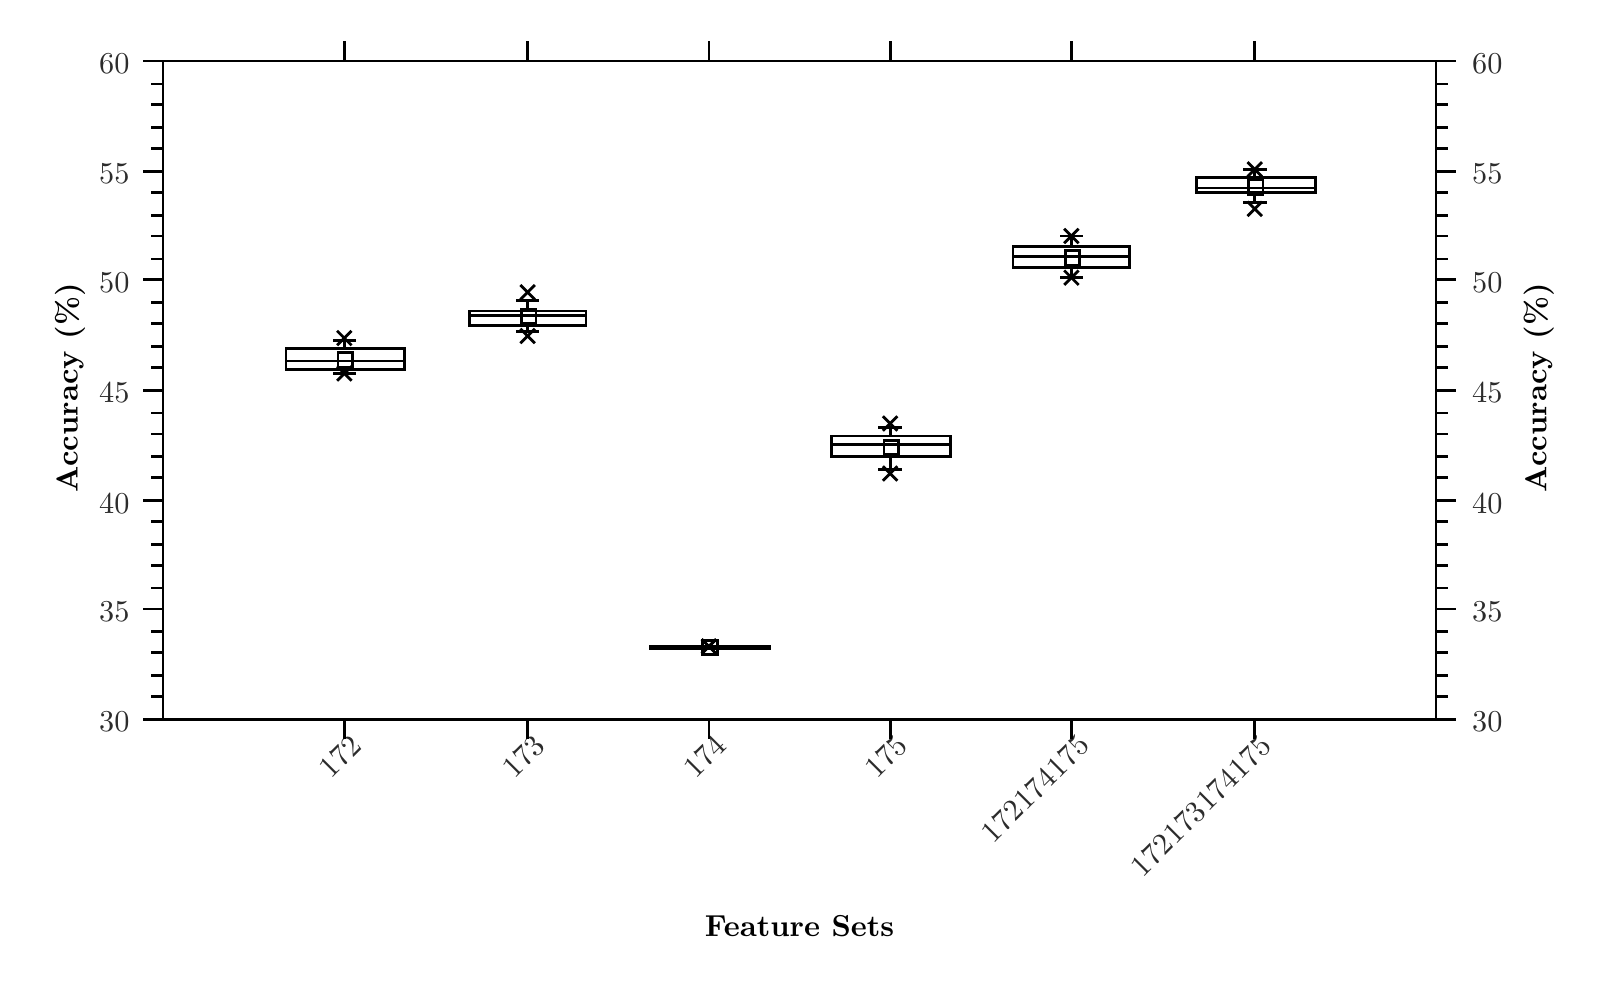
\begin{tikzpicture}{0pt}{0pt}{742pt}{452pt}
	\clip(0pt,452pt) -- (558.587pt,452pt) -- (558.587pt,111.729pt) -- (0pt,111.729pt) -- (0pt,452pt);
\begin{scope}
	\clip(48.9328pt,439.955pt) -- (508.901pt,439.955pt) -- (508.901pt,202.066pt) -- (48.9328pt,202.066pt) -- (48.9328pt,439.955pt);
	\color[rgb]{0,0,0}
	\draw[line width=1pt, line join=miter, line cap=rect](93.3487pt,336.067pt) -- (136.259pt,336.067pt) -- (136.259pt,328.539pt) -- (93.3487pt,328.539pt) -- (93.3487pt,336.067pt);
	\color[rgb]{0,0,0}
	\draw[line width=1pt, line join=miter, line cap=rect](110.663pt,327.033pt) -- (118.192pt,327.033pt);
	\draw[line width=1pt, line join=miter, line cap=rect](110.663pt,339.078pt) -- (118.192pt,339.078pt);
	\draw[line width=1pt, line join=miter, line cap=rect](114.427pt,339.078pt) -- (114.427pt,336.067pt);
	\draw[line width=1pt, line join=miter, line cap=rect](114.427pt,327.033pt) -- (114.427pt,328.539pt);
	\draw[line width=1pt, line join=miter, line cap=rect](93.3487pt,331.55pt) -- (135.506pt,331.55pt);
	\draw[line width=1pt, line join=miter, line cap=rect](112.169pt,329.292pt) -- (116.686pt,324.775pt);
	\draw[line width=1pt, line join=miter, line cap=rect](112.169pt,324.775pt) -- (116.686pt,329.292pt);
	\draw[line width=1pt, line join=miter, line cap=rect](112.169pt,342.089pt) -- (116.686pt,337.572pt);
	\draw[line width=1pt, line join=miter, line cap=rect](112.169pt,337.572pt) -- (116.686pt,342.089pt);
	\draw[line width=1pt, line join=miter, line cap=rect](112.169pt,334.561pt) -- (117.439pt,334.561pt) -- (117.439pt,329.292pt) -- (112.169pt,329.292pt) -- (112.169pt,334.561pt);
	\draw[line width=1pt, line join=miter, line cap=rect](159.596pt,349.618pt) -- (201.754pt,349.618pt) -- (201.754pt,344.348pt) -- (159.596pt,344.348pt) -- (159.596pt,349.618pt);
	\draw[line width=1pt, line join=miter, line cap=rect](176.911pt,342.089pt) -- (184.439pt,342.089pt);
	\draw[line width=1pt, line join=miter, line cap=rect](176.911pt,353.382pt) -- (184.439pt,353.382pt);
	\draw[line width=1pt, line join=miter, line cap=rect](180.675pt,353.382pt) -- (180.675pt,349.618pt);
	\draw[line width=1pt, line join=miter, line cap=rect](180.675pt,342.089pt) -- (180.675pt,344.348pt);
	\draw[line width=1pt, line join=miter, line cap=rect](159.596pt,348.112pt) -- (201.754pt,348.112pt);
	\draw[line width=1pt, line join=miter, line cap=rect](178.417pt,342.842pt) -- (182.933pt,338.325pt);
	\draw[line width=1pt, line join=miter, line cap=rect](178.417pt,338.325pt) -- (182.933pt,342.842pt);
	\draw[line width=1pt, line join=miter, line cap=rect](178.417pt,358.651pt) -- (182.933pt,354.134pt);
	\draw[line width=1pt, line join=miter, line cap=rect](178.417pt,354.134pt) -- (182.933pt,358.651pt);
	\draw[line width=1pt, line join=miter, line cap=rect](178.417pt,350.37pt) -- (183.686pt,350.37pt) -- (183.686pt,345.101pt) -- (178.417pt,345.101pt) -- (178.417pt,350.37pt);
	\draw[line width=1pt, line join=miter, line cap=rect](225.091pt,228.415pt) -- (268.001pt,228.415pt) -- (268.001pt,227.662pt) -- (225.091pt,227.662pt) -- (225.091pt,228.415pt);
	\draw[line width=1pt, line join=miter, line cap=rect](242.406pt,228.415pt) -- (249.934pt,228.415pt);
	\draw[line width=1pt, line join=miter, line cap=rect](242.406pt,228.415pt) -- (249.934pt,228.415pt);
	\draw[line width=1pt, line join=miter, line cap=rect](225.091pt,228.415pt) -- (267.248pt,228.415pt);
	\draw[line width=1pt, line join=miter, line cap=rect](243.911pt,230.673pt) -- (248.428pt,226.156pt);
	\draw[line width=1pt, line join=miter, line cap=rect](243.911pt,226.156pt) -- (248.428pt,230.673pt);
	\draw[line width=1pt, line join=miter, line cap=rect](243.911pt,230.673pt) -- (248.428pt,226.156pt);
	\draw[line width=1pt, line join=miter, line cap=rect](243.911pt,226.156pt) -- (248.428pt,230.673pt);
	\draw[line width=1pt, line join=miter, line cap=rect](243.911pt,230.673pt) -- (249.181pt,230.673pt) -- (249.181pt,225.403pt) -- (243.911pt,225.403pt) -- (243.911pt,230.673pt);
	\draw[line width=1pt, line join=miter, line cap=rect](290.586pt,304.449pt) -- (333.496pt,304.449pt) -- (333.496pt,296.921pt) -- (290.586pt,296.921pt) -- (290.586pt,304.449pt);
	\draw[line width=1pt, line join=miter, line cap=rect](307.9pt,292.404pt) -- (315.428pt,292.404pt);
	\draw[line width=1pt, line join=miter, line cap=rect](307.9pt,307.46pt) -- (315.428pt,307.46pt);
	\draw[line width=1pt, line join=miter, line cap=rect](311.664pt,307.46pt) -- (311.664pt,304.449pt);
	\draw[line width=1pt, line join=miter, line cap=rect](311.664pt,292.404pt) -- (311.664pt,296.921pt);
	\draw[line width=1pt, line join=miter, line cap=rect](290.586pt,301.438pt) -- (332.743pt,301.438pt);
	\draw[line width=1pt, line join=miter, line cap=rect](309.406pt,293.157pt) -- (313.923pt,288.64pt);
	\draw[line width=1pt, line join=miter, line cap=rect](309.406pt,288.64pt) -- (313.923pt,293.157pt);
	\draw[line width=1pt, line join=miter, line cap=rect](309.406pt,311.224pt) -- (313.923pt,306.707pt);
	\draw[line width=1pt, line join=miter, line cap=rect](309.406pt,306.707pt) -- (313.923pt,311.224pt);
	\draw[line width=1pt, line join=miter, line cap=rect](309.406pt,302.943pt) -- (314.676pt,302.943pt) -- (314.676pt,297.673pt) -- (309.406pt,297.673pt) -- (309.406pt,302.943pt);
	\draw[line width=1pt, line join=miter, line cap=rect](356.08pt,372.955pt) -- (398.238pt,372.955pt) -- (398.238pt,365.427pt) -- (356.08pt,365.427pt) -- (356.08pt,372.955pt);
	\draw[line width=1pt, line join=miter, line cap=rect](373.395pt,361.663pt) -- (380.923pt,361.663pt);
	\draw[line width=1pt, line join=miter, line cap=rect](373.395pt,376.719pt) -- (380.923pt,376.719pt);
	\draw[line width=1pt, line join=miter, line cap=rect](377.159pt,376.719pt) -- (377.159pt,372.955pt);
	\draw[line width=1pt, line join=miter, line cap=rect](377.159pt,361.663pt) -- (377.159pt,365.427pt);
	\draw[line width=1pt, line join=miter, line cap=rect](356.08pt,369.191pt) -- (398.238pt,369.191pt);
	\draw[line width=1pt, line join=miter, line cap=rect](374.901pt,363.921pt) -- (379.418pt,359.404pt);
	\draw[line width=1pt, line join=miter, line cap=rect](374.901pt,359.404pt) -- (379.418pt,363.921pt);
	\draw[line width=1pt, line join=miter, line cap=rect](374.901pt,378.977pt) -- (379.418pt,374.46pt);
	\draw[line width=1pt, line join=miter, line cap=rect](374.901pt,374.46pt) -- (379.418pt,378.977pt);
	\draw[line width=1pt, line join=miter, line cap=rect](374.901pt,371.449pt) -- (380.17pt,371.449pt) -- (380.17pt,366.179pt) -- (374.901pt,366.179pt) -- (374.901pt,371.449pt);
	\draw[line width=1pt, line join=miter, line cap=rect](422.328pt,397.798pt) -- (465.238pt,397.798pt) -- (465.238pt,392.528pt) -- (422.328pt,392.528pt) -- (422.328pt,397.798pt);
	\draw[line width=1pt, line join=miter, line cap=rect](439.642pt,388.764pt) -- (447.171pt,388.764pt);
	\draw[line width=1pt, line join=miter, line cap=rect](439.642pt,400.809pt) -- (447.171pt,400.809pt);
	\draw[line width=1pt, line join=miter, line cap=rect](443.407pt,400.809pt) -- (443.407pt,397.798pt);
	\draw[line width=1pt, line join=miter, line cap=rect](443.407pt,388.764pt) -- (443.407pt,392.528pt);
	\draw[line width=1pt, line join=miter, line cap=rect](422.328pt,394.033pt) -- (464.485pt,394.033pt);
	\draw[line width=1pt, line join=miter, line cap=rect](441.148pt,388.764pt) -- (445.665pt,384.247pt);
	\draw[line width=1pt, line join=miter, line cap=rect](441.148pt,384.247pt) -- (445.665pt,388.764pt);
	\draw[line width=1pt, line join=miter, line cap=rect](441.148pt,403.067pt) -- (445.665pt,398.55pt);
	\draw[line width=1pt, line join=miter, line cap=rect](441.148pt,398.55pt) -- (445.665pt,403.067pt);
	\draw[line width=1pt, line join=miter, line cap=rect](441.148pt,397.045pt) -- (446.418pt,397.045pt) -- (446.418pt,391.775pt) -- (441.148pt,391.775pt) -- (441.148pt,397.045pt);
\end{scope}
\begin{scope}
	\color[rgb]{0,0,0}
	\pgftext[center, base, at={\pgfpoint{18.0675pt}{321.763pt}},rotate=90]{\fontsize{11}{0}\selectfont{\textbf{Accuracy (\%)}}}
	\color[rgb]{0.172549,0.172549,0.172549}
	\pgftext[center, base, at={\pgfpoint{31.3358pt}{197.549pt}}]{\fontsize{11}{0}\selectfont{30}}
	\pgftext[center, base, at={\pgfpoint{31.3358pt}{237.448pt}}]{\fontsize{11}{0}\selectfont{35}}
	\pgftext[center, base, at={\pgfpoint{31.3358pt}{276.595pt}}]{\fontsize{11}{0}\selectfont{40}}
	\pgftext[center, base, at={\pgfpoint{31.3358pt}{316.494pt}}]{\fontsize{11}{0}\selectfont{45}}
	\pgftext[center, base, at={\pgfpoint{31.3358pt}{356.393pt}}]{\fontsize{11}{0}\selectfont{50}}
	\pgftext[center, base, at={\pgfpoint{31.3358pt}{395.539pt}}]{\fontsize{11}{0}\selectfont{55}}
	\pgftext[center, base, at={\pgfpoint{31.3358pt}{435.438pt}}]{\fontsize{11}{0}\selectfont{60}}
	\color[rgb]{0,0,0}
	\draw[line width=1pt, line join=bevel, line cap=rect](48.9328pt,210.347pt) -- (45.1688pt,210.347pt);
	\draw[line width=1pt, line join=bevel, line cap=rect](48.9328pt,217.875pt) -- (45.1688pt,217.875pt);
	\draw[line width=1pt, line join=bevel, line cap=rect](48.9328pt,226.156pt) -- (45.1688pt,226.156pt);
	\draw[line width=1pt, line join=bevel, line cap=rect](48.9328pt,233.684pt) -- (45.1688pt,233.684pt);
	\draw[line width=1pt, line join=bevel, line cap=rect](48.9328pt,249.493pt) -- (45.1688pt,249.493pt);
	\draw[line width=1pt, line join=bevel, line cap=rect](48.9328pt,257.774pt) -- (45.1688pt,257.774pt);
	\draw[line width=1pt, line join=bevel, line cap=rect](48.9328pt,265.303pt) -- (45.1688pt,265.303pt);
	\draw[line width=1pt, line join=bevel, line cap=rect](48.9328pt,273.583pt) -- (45.1688pt,273.583pt);
	\draw[line width=1pt, line join=bevel, line cap=rect](48.9328pt,289.393pt) -- (45.1688pt,289.393pt);
	\draw[line width=1pt, line join=bevel, line cap=rect](48.9328pt,296.921pt) -- (45.1688pt,296.921pt);
	\draw[line width=1pt, line join=bevel, line cap=rect](48.9328pt,305.202pt) -- (45.1688pt,305.202pt);
	\draw[line width=1pt, line join=bevel, line cap=rect](48.9328pt,312.73pt) -- (45.1688pt,312.73pt);
	\draw[line width=1pt, line join=bevel, line cap=rect](48.9328pt,329.292pt) -- (45.1688pt,329.292pt);
	\draw[line width=1pt, line join=bevel, line cap=rect](48.9328pt,336.82pt) -- (45.1688pt,336.82pt);
	\draw[line width=1pt, line join=bevel, line cap=rect](48.9328pt,345.101pt) -- (45.1688pt,345.101pt);
	\draw[line width=1pt, line join=bevel, line cap=rect](48.9328pt,352.629pt) -- (45.1688pt,352.629pt);
	\draw[line width=1pt, line join=bevel, line cap=rect](48.9328pt,368.438pt) -- (45.1688pt,368.438pt);
	\draw[line width=1pt, line join=bevel, line cap=rect](48.9328pt,376.719pt) -- (45.1688pt,376.719pt);
	\draw[line width=1pt, line join=bevel, line cap=rect](48.9328pt,384.247pt) -- (45.1688pt,384.247pt);
	\draw[line width=1pt, line join=bevel, line cap=rect](48.9328pt,392.528pt) -- (45.1688pt,392.528pt);
	\draw[line width=1pt, line join=bevel, line cap=rect](48.9328pt,408.337pt) -- (45.1688pt,408.337pt);
	\draw[line width=1pt, line join=bevel, line cap=rect](48.9328pt,415.865pt) -- (45.1688pt,415.865pt);
	\draw[line width=1pt, line join=bevel, line cap=rect](48.9328pt,424.146pt) -- (45.1688pt,424.146pt);
	\draw[line width=1pt, line join=bevel, line cap=rect](48.9328pt,431.674pt) -- (45.1688pt,431.674pt);
	\draw[line width=1pt, line join=bevel, line cap=rect](48.9328pt,202.066pt) -- (42.1575pt,202.066pt);
	\draw[line width=1pt, line join=bevel, line cap=rect](48.9328pt,241.965pt) -- (42.1575pt,241.965pt);
	\draw[line width=1pt, line join=bevel, line cap=rect](48.9328pt,281.112pt) -- (42.1575pt,281.112pt);
	\draw[line width=1pt, line join=bevel, line cap=rect](48.9328pt,321.011pt) -- (42.1575pt,321.011pt);
	\draw[line width=1pt, line join=bevel, line cap=rect](48.9328pt,360.91pt) -- (42.1575pt,360.91pt);
	\draw[line width=1pt, line join=bevel, line cap=rect](48.9328pt,400.056pt) -- (42.1575pt,400.056pt);
	\draw[line width=1pt, line join=bevel, line cap=rect](48.9328pt,439.955pt) -- (42.1575pt,439.955pt);
	\draw[line width=1pt, line join=bevel, line cap=rect](48.9328pt,439.955pt) -- (48.9328pt,202.066pt);
	\pgftext[center, base, at={\pgfpoint{548.8pt}{321.763pt}},rotate=90]{\fontsize{11}{0}\selectfont{\textbf{Accuracy (\%)}}}
	\color[rgb]{0.172549,0.172549,0.172549}
	\pgftext[center, base, at={\pgfpoint{527.439pt}{197.549pt}}]{\fontsize{11}{0}\selectfont{30}}
	\pgftext[center, base, at={\pgfpoint{527.439pt}{237.448pt}}]{\fontsize{11}{0}\selectfont{35}}
	\pgftext[center, base, at={\pgfpoint{527.439pt}{276.595pt}}]{\fontsize{11}{0}\selectfont{40}}
	\pgftext[center, base, at={\pgfpoint{527.439pt}{316.494pt}}]{\fontsize{11}{0}\selectfont{45}}
	\pgftext[center, base, at={\pgfpoint{527.439pt}{356.393pt}}]{\fontsize{11}{0}\selectfont{50}}
	\pgftext[center, base, at={\pgfpoint{527.439pt}{395.539pt}}]{\fontsize{11}{0}\selectfont{55}}
	\pgftext[center, base, at={\pgfpoint{527.439pt}{435.438pt}}]{\fontsize{11}{0}\selectfont{60}}
	\color[rgb]{0,0,0}
	\draw[line width=1pt, line join=bevel, line cap=rect](508.901pt,210.347pt) -- (512.665pt,210.347pt);
	\draw[line width=1pt, line join=bevel, line cap=rect](508.901pt,217.875pt) -- (512.665pt,217.875pt);
	\draw[line width=1pt, line join=bevel, line cap=rect](508.901pt,226.156pt) -- (512.665pt,226.156pt);
	\draw[line width=1pt, line join=bevel, line cap=rect](508.901pt,233.684pt) -- (512.665pt,233.684pt);
	\draw[line width=1pt, line join=bevel, line cap=rect](508.901pt,249.493pt) -- (512.665pt,249.493pt);
	\draw[line width=1pt, line join=bevel, line cap=rect](508.901pt,257.774pt) -- (512.665pt,257.774pt);
	\draw[line width=1pt, line join=bevel, line cap=rect](508.901pt,265.303pt) -- (512.665pt,265.303pt);
	\draw[line width=1pt, line join=bevel, line cap=rect](508.901pt,273.583pt) -- (512.665pt,273.583pt);
	\draw[line width=1pt, line join=bevel, line cap=rect](508.901pt,289.393pt) -- (512.665pt,289.393pt);
	\draw[line width=1pt, line join=bevel, line cap=rect](508.901pt,296.921pt) -- (512.665pt,296.921pt);
	\draw[line width=1pt, line join=bevel, line cap=rect](508.901pt,305.202pt) -- (512.665pt,305.202pt);
	\draw[line width=1pt, line join=bevel, line cap=rect](508.901pt,312.73pt) -- (512.665pt,312.73pt);
	\draw[line width=1pt, line join=bevel, line cap=rect](508.901pt,329.292pt) -- (512.665pt,329.292pt);
	\draw[line width=1pt, line join=bevel, line cap=rect](508.901pt,336.82pt) -- (512.665pt,336.82pt);
	\draw[line width=1pt, line join=bevel, line cap=rect](508.901pt,345.101pt) -- (512.665pt,345.101pt);
	\draw[line width=1pt, line join=bevel, line cap=rect](508.901pt,352.629pt) -- (512.665pt,352.629pt);
	\draw[line width=1pt, line join=bevel, line cap=rect](508.901pt,368.438pt) -- (512.665pt,368.438pt);
	\draw[line width=1pt, line join=bevel, line cap=rect](508.901pt,376.719pt) -- (512.665pt,376.719pt);
	\draw[line width=1pt, line join=bevel, line cap=rect](508.901pt,384.247pt) -- (512.665pt,384.247pt);
	\draw[line width=1pt, line join=bevel, line cap=rect](508.901pt,392.528pt) -- (512.665pt,392.528pt);
	\draw[line width=1pt, line join=bevel, line cap=rect](508.901pt,408.337pt) -- (512.665pt,408.337pt);
	\draw[line width=1pt, line join=bevel, line cap=rect](508.901pt,415.865pt) -- (512.665pt,415.865pt);
	\draw[line width=1pt, line join=bevel, line cap=rect](508.901pt,424.146pt) -- (512.665pt,424.146pt);
	\draw[line width=1pt, line join=bevel, line cap=rect](508.901pt,431.674pt) -- (512.665pt,431.674pt);
	\draw[line width=1pt, line join=bevel, line cap=rect](508.901pt,202.066pt) -- (515.677pt,202.066pt);
	\draw[line width=1pt, line join=bevel, line cap=rect](508.901pt,241.965pt) -- (515.677pt,241.965pt);
	\draw[line width=1pt, line join=bevel, line cap=rect](508.901pt,281.112pt) -- (515.677pt,281.112pt);
	\draw[line width=1pt, line join=bevel, line cap=rect](508.901pt,321.011pt) -- (515.677pt,321.011pt);
	\draw[line width=1pt, line join=bevel, line cap=rect](508.901pt,360.91pt) -- (515.677pt,360.91pt);
	\draw[line width=1pt, line join=bevel, line cap=rect](508.901pt,400.056pt) -- (515.677pt,400.056pt);
	\draw[line width=1pt, line join=bevel, line cap=rect](508.901pt,439.955pt) -- (515.677pt,439.955pt);
	\draw[line width=1pt, line join=bevel, line cap=rect](508.901pt,439.955pt) -- (508.901pt,202.066pt);
	\pgftext[center, base, at={\pgfpoint{278.911pt}{123.774pt}}]{\fontsize{11}{0}\selectfont{\textbf{Feature Sets}}}
	\color[rgb]{0.172549,0.172549,0.172549}
	\pgftext[center, base, at={\pgfpoint{115.392pt}{186.104pt}},rotate=45]{\fontsize{11}{0}\selectfont{\ding{172}}}
	\pgftext[center, base, at={\pgfpoint{181.64pt}{186.104pt}},rotate=45]{\fontsize{11}{0}\selectfont{\ding{173}}}
	\pgftext[center, base, at={\pgfpoint{247.135pt}{186.104pt}},rotate=45]{\fontsize{11}{0}\selectfont{\ding{174}}}
	\pgftext[center, base, at={\pgfpoint{312.629pt}{186.104pt}},rotate=45]{\fontsize{11}{0}\selectfont{\ding{175}}}
	\pgftext[center, base, at={\pgfpoint{354.702pt}{162.682pt}},rotate=45]{\fontsize{11}{0}\selectfont{\ding{172}}}
	\pgftext[center, base, at={\pgfpoint{366.513pt}{174.493pt}},rotate=45]{\fontsize{11}{0}\selectfont{\ding{174}}}
	\pgftext[center, base, at={\pgfpoint{378.324pt}{186.303pt}},rotate=45]{\fontsize{11}{0}\selectfont{\ding{175}}}
	\pgftext[center, base, at={\pgfpoint{408.706pt}{150.439pt}},rotate=45]{\fontsize{11}{0}\selectfont{\ding{172}}}
	\pgftext[center, base, at={\pgfpoint{420.517pt}{162.249pt}},rotate=45]{\fontsize{11}{0}\selectfont{\ding{173}}}
	\pgftext[center, base, at={\pgfpoint{432.328pt}{174.06pt}},rotate=45]{\fontsize{11}{0}\selectfont{\ding{174}}}
	\pgftext[center, base, at={\pgfpoint{444.139pt}{185.871pt}},rotate=45]{\fontsize{11}{0}\selectfont{\ding{175}}}
	\color[rgb]{0,0,0}
	\draw[line width=1pt, line join=bevel, line cap=rect](114.427pt,202.066pt) -- (114.427pt,195.291pt);
	\draw[line width=1pt, line join=bevel, line cap=rect](180.675pt,202.066pt) -- (180.675pt,195.291pt);
	\draw[line width=1pt, line join=bevel, line cap=rect](246.17pt,202.066pt) -- (246.17pt,195.291pt);
	\draw[line width=1pt, line join=bevel, line cap=rect](311.664pt,202.066pt) -- (311.664pt,195.291pt);
	\draw[line width=1pt, line join=bevel, line cap=rect](377.159pt,202.066pt) -- (377.159pt,195.291pt);
	\draw[line width=1pt, line join=bevel, line cap=rect](443.407pt,202.066pt) -- (443.407pt,195.291pt);
	\draw[line width=1pt, line join=bevel, line cap=rect](48.9328pt,202.066pt) -- (508.901pt,202.066pt);
	\draw[line width=1pt, line join=bevel, line cap=rect](114.427pt,439.955pt) -- (114.427pt,446.73pt);
	\draw[line width=1pt, line join=bevel, line cap=rect](180.675pt,439.955pt) -- (180.675pt,446.73pt);
	\draw[line width=1pt, line join=bevel, line cap=rect](246.17pt,439.955pt) -- (246.17pt,446.73pt);
	\draw[line width=1pt, line join=bevel, line cap=rect](311.664pt,439.955pt) -- (311.664pt,446.73pt);
	\draw[line width=1pt, line join=bevel, line cap=rect](377.159pt,439.955pt) -- (377.159pt,446.73pt);
	\draw[line width=1pt, line join=bevel, line cap=rect](443.407pt,439.955pt) -- (443.407pt,446.73pt);
	\draw[line width=1pt, line join=bevel, line cap=rect](48.9328pt,439.955pt) -- (508.901pt,439.955pt);
\end{scope}
\end{tikzpicture}

  \end{adjustbox}
  \caption{Method-level cross-validation accuracy of feature sets on the \emph{all} subject.}
  \vspace{2mm}
  \hrule
  \label{fig:all_cross_validation_features_method_graph}
\end{figure}

We use the LIBSVM~\cite{CL11} library to perform 10-fold cross-validation. To evaluate the cross-validation accuracy of the acquired data we randomly under-sample the data to balance the amount of data points within each category. We utilize 191 class-level and 1104 method-level source code units  data points from each category, these values are chosen to maximize the number of instances of the minority category using random under-sampling.

Recall that we have a set of features (i.e., attributes for our vector in the \gls{svm}) as listed in Table~\ref{tab:feature_sets}. We explore the cross-validation accuracy using different feature sets (i.e., \ding{172}, \ding{173}, \ding{174}, \ding{175}) in Figures~\ref{fig:all_cross_validation_features_class_graph}~and~\ref{fig:all_cross_validation_features_method_graph}. The cross-validation accuracy of class- and method-level source code units were performed on the collective \emph{all} subject over ten executions to account for random undersampling of our data. To assess our cross-validation accuracy, we use random selection as our baseline. In our case, since we undersample our three categories, random selection will have an accuracy of 33.3333\%. We can see that all feature sets are able to outperform random which indicates that there is some predictive power in the selected feature sets\footnote{Feature set \ding{174} for method-level source code units (Figure~\ref{fig:all_cross_validation_features_method_graph}) does not add any value (as it is specifically tailor for class-level source code units), and thus performs as random.}. We include a subset of all features (feature sets \ding{172} \ding{174} \ding{175}) to show the effects of merging only the source code and test suite metrics (excluding coverage feature set \ding{173}). We can clearly see that by using all feature sets together we can acquire higher cross-validation accuracy then using the feature sets alone. This observation supports our intuition that using various source code and test suite metrics together can predict the mutation scores of source code units well.

\begin{figure}[!tb]
  \centering
  \begin{adjustbox}{max size={.95\textwidth}{.95\textheight}}
    \begin{tikzpicture}{0pt}{0pt}{742pt}{452pt}
	\clip(0pt,452pt) -- (558.587pt,452pt) -- (558.587pt,111.729pt) -- (0pt,111.729pt) -- (0pt,452pt);
\begin{scope}
	\clip(49.6856pt,439.202pt) -- (509.654pt,439.202pt) -- (509.654pt,217.123pt) -- (49.6856pt,217.123pt) -- (49.6856pt,439.202pt);
	\color[rgb]{0,0,0}
	\draw[line width=1pt, line join=miter, line cap=rect](80.5509pt,344.348pt) -- (110.663pt,344.348pt) -- (110.663pt,308.966pt) -- (80.5509pt,308.966pt) -- (80.5509pt,344.348pt);
	\color[rgb]{0,0,0}
	\draw[line width=1pt, line join=miter, line cap=rect](92.5959pt,284.123pt) -- (98.6184pt,284.123pt);
	\draw[line width=1pt, line join=miter, line cap=rect](92.5959pt,381.236pt) -- (98.6184pt,381.236pt);
	\draw[line width=1pt, line join=miter, line cap=rect](95.6072pt,381.236pt) -- (95.6072pt,344.348pt);
	\draw[line width=1pt, line join=miter, line cap=rect](95.6072pt,284.123pt) -- (95.6072pt,308.966pt);
	\draw[line width=1pt, line join=miter, line cap=rect](80.5509pt,309.718pt) -- (110.663pt,309.718pt);
	\draw[line width=1pt, line join=miter, line cap=rect](93.3487pt,265.303pt) -- (97.8656pt,260.786pt);
	\draw[line width=1pt, line join=miter, line cap=rect](93.3487pt,260.786pt) -- (97.8656pt,265.303pt);
	\draw[line width=1pt, line join=miter, line cap=rect](93.3487pt,404.573pt) -- (97.8656pt,400.056pt);
	\draw[line width=1pt, line join=miter, line cap=rect](93.3487pt,400.056pt) -- (97.8656pt,404.573pt);
	\draw[line width=1pt, line join=miter, line cap=rect](93.3487pt,325.528pt) -- (98.6184pt,325.528pt) -- (98.6184pt,320.258pt) -- (93.3487pt,320.258pt) -- (93.3487pt,325.528pt);
	\draw[line width=1pt, line join=miter, line cap=rect](126.472pt,380.483pt) -- (156.585pt,380.483pt) -- (156.585pt,371.449pt) -- (126.472pt,371.449pt) -- (126.472pt,380.483pt);
	\draw[line width=1pt, line join=miter, line cap=rect](138.518pt,363.921pt) -- (144.54pt,363.921pt);
	\draw[line width=1pt, line join=miter, line cap=rect](138.518pt,381.988pt) -- (144.54pt,381.988pt);
	\draw[line width=1pt, line join=miter, line cap=rect](141.529pt,381.988pt) -- (141.529pt,380.483pt);
	\draw[line width=1pt, line join=miter, line cap=rect](141.529pt,363.921pt) -- (141.529pt,371.449pt);
	\draw[line width=1pt, line join=miter, line cap=rect](126.472pt,376.719pt) -- (156.585pt,376.719pt);
	\draw[line width=1pt, line join=miter, line cap=rect](139.27pt,363.168pt) -- (143.787pt,358.651pt);
	\draw[line width=1pt, line join=miter, line cap=rect](139.27pt,358.651pt) -- (143.787pt,363.168pt);
	\draw[line width=1pt, line join=miter, line cap=rect](139.27pt,384.247pt) -- (143.787pt,379.73pt);
	\draw[line width=1pt, line join=miter, line cap=rect](139.27pt,379.73pt) -- (143.787pt,384.247pt);
	\draw[line width=1pt, line join=miter, line cap=rect](139.27pt,377.472pt) -- (144.54pt,377.472pt) -- (144.54pt,372.202pt) -- (139.27pt,372.202pt) -- (139.27pt,377.472pt);
	\draw[line width=1pt, line join=miter, line cap=rect](172.394pt,369.943pt) -- (202.507pt,369.943pt) -- (202.507pt,348.112pt) -- (172.394pt,348.112pt) -- (172.394pt,369.943pt);
	\draw[line width=1pt, line join=miter, line cap=rect](184.439pt,338.325pt) -- (190.462pt,338.325pt);
	\draw[line width=1pt, line join=miter, line cap=rect](184.439pt,380.483pt) -- (190.462pt,380.483pt);
	\draw[line width=1pt, line join=miter, line cap=rect](187.45pt,380.483pt) -- (187.45pt,369.943pt);
	\draw[line width=1pt, line join=miter, line cap=rect](187.45pt,338.325pt) -- (187.45pt,348.112pt);
	\draw[line width=1pt, line join=miter, line cap=rect](172.394pt,359.404pt) -- (202.507pt,359.404pt);
	\draw[line width=1pt, line join=miter, line cap=rect](185.192pt,340.584pt) -- (189.709pt,336.067pt);
	\draw[line width=1pt, line join=miter, line cap=rect](185.192pt,336.067pt) -- (189.709pt,340.584pt);
	\draw[line width=1pt, line join=miter, line cap=rect](185.192pt,382.741pt) -- (189.709pt,378.224pt);
	\draw[line width=1pt, line join=miter, line cap=rect](185.192pt,378.224pt) -- (189.709pt,382.741pt);
	\draw[line width=1pt, line join=miter, line cap=rect](185.192pt,361.663pt) -- (190.462pt,361.663pt) -- (190.462pt,356.393pt) -- (185.192pt,356.393pt) -- (185.192pt,361.663pt);
	\draw[line width=1pt, line join=miter, line cap=rect](218.316pt,366.179pt) -- (248.428pt,366.179pt) -- (248.428pt,352.629pt) -- (218.316pt,352.629pt) -- (218.316pt,366.179pt);
	\draw[line width=1pt, line join=miter, line cap=rect](230.361pt,340.584pt) -- (236.383pt,340.584pt);
	\draw[line width=1pt, line join=miter, line cap=rect](230.361pt,371.449pt) -- (236.383pt,371.449pt);
	\draw[line width=1pt, line join=miter, line cap=rect](233.372pt,371.449pt) -- (233.372pt,366.179pt);
	\draw[line width=1pt, line join=miter, line cap=rect](233.372pt,340.584pt) -- (233.372pt,352.629pt);
	\draw[line width=1pt, line join=miter, line cap=rect](218.316pt,357.898pt) -- (248.428pt,357.898pt);
	\draw[line width=1pt, line join=miter, line cap=rect](231.113pt,342.842pt) -- (235.63pt,338.325pt);
	\draw[line width=1pt, line join=miter, line cap=rect](231.113pt,338.325pt) -- (235.63pt,342.842pt);
	\draw[line width=1pt, line join=miter, line cap=rect](231.113pt,377.472pt) -- (235.63pt,372.955pt);
	\draw[line width=1pt, line join=miter, line cap=rect](231.113pt,372.955pt) -- (235.63pt,377.472pt);
	\draw[line width=1pt, line join=miter, line cap=rect](231.113pt,360.157pt) -- (236.383pt,360.157pt) -- (236.383pt,354.887pt) -- (231.113pt,354.887pt) -- (231.113pt,360.157pt);
	\draw[line width=1pt, line join=miter, line cap=rect](264.99pt,388.011pt) -- (295.103pt,388.011pt) -- (295.103pt,365.427pt) -- (264.99pt,365.427pt) -- (264.99pt,388.011pt);
	\draw[line width=1pt, line join=miter, line cap=rect](277.035pt,354.887pt) -- (283.058pt,354.887pt);
	\draw[line width=1pt, line join=miter, line cap=rect](277.035pt,398.55pt) -- (283.058pt,398.55pt);
	\draw[line width=1pt, line join=miter, line cap=rect](280.046pt,398.55pt) -- (280.046pt,388.011pt);
	\draw[line width=1pt, line join=miter, line cap=rect](280.046pt,354.887pt) -- (280.046pt,365.427pt);
	\draw[line width=1pt, line join=miter, line cap=rect](264.99pt,378.224pt) -- (295.103pt,378.224pt);
	\draw[line width=1pt, line join=miter, line cap=rect](277.788pt,351.876pt) -- (282.305pt,347.359pt);
	\draw[line width=1pt, line join=miter, line cap=rect](277.788pt,347.359pt) -- (282.305pt,351.876pt);
	\draw[line width=1pt, line join=miter, line cap=rect](277.788pt,404.573pt) -- (282.305pt,400.056pt);
	\draw[line width=1pt, line join=miter, line cap=rect](277.788pt,400.056pt) -- (282.305pt,404.573pt);
	\draw[line width=1pt, line join=miter, line cap=rect](277.788pt,379.73pt) -- (283.058pt,379.73pt) -- (283.058pt,374.46pt) -- (277.788pt,374.46pt) -- (277.788pt,379.73pt);
	\draw[line width=1pt, line join=miter, line cap=rect](310.912pt,384.247pt) -- (341.024pt,384.247pt) -- (341.024pt,357.898pt) -- (310.912pt,357.898pt) -- (310.912pt,384.247pt);
	\draw[line width=1pt, line join=miter, line cap=rect](322.957pt,342.842pt) -- (328.979pt,342.842pt);
	\draw[line width=1pt, line join=miter, line cap=rect](322.957pt,400.056pt) -- (328.979pt,400.056pt);
	\draw[line width=1pt, line join=miter, line cap=rect](325.968pt,400.056pt) -- (325.968pt,384.247pt);
	\draw[line width=1pt, line join=miter, line cap=rect](325.968pt,342.842pt) -- (325.968pt,357.898pt);
	\draw[line width=1pt, line join=miter, line cap=rect](310.912pt,368.438pt) -- (341.024pt,368.438pt);
	\draw[line width=1pt, line join=miter, line cap=rect](323.709pt,342.842pt) -- (328.226pt,338.325pt);
	\draw[line width=1pt, line join=miter, line cap=rect](323.709pt,338.325pt) -- (328.226pt,342.842pt);
	\draw[line width=1pt, line join=miter, line cap=rect](323.709pt,404.573pt) -- (328.226pt,400.056pt);
	\draw[line width=1pt, line join=miter, line cap=rect](323.709pt,400.056pt) -- (328.226pt,404.573pt);
	\draw[line width=1pt, line join=miter, line cap=rect](323.709pt,372.955pt) -- (328.979pt,372.955pt) -- (328.979pt,367.685pt) -- (323.709pt,367.685pt) -- (323.709pt,372.955pt);
	\draw[line width=1pt, line join=miter, line cap=rect](356.833pt,381.236pt) -- (386.946pt,381.236pt) -- (386.946pt,349.618pt) -- (356.833pt,349.618pt) -- (356.833pt,381.236pt);
	\draw[line width=1pt, line join=miter, line cap=rect](368.878pt,333.056pt) -- (374.901pt,333.056pt);
	\draw[line width=1pt, line join=miter, line cap=rect](368.878pt,391.022pt) -- (374.901pt,391.022pt);
	\draw[line width=1pt, line join=miter, line cap=rect](371.889pt,391.022pt) -- (371.889pt,381.236pt);
	\draw[line width=1pt, line join=miter, line cap=rect](371.889pt,333.056pt) -- (371.889pt,349.618pt);
	\draw[line width=1pt, line join=miter, line cap=rect](356.833pt,355.64pt) -- (386.946pt,355.64pt);
	\draw[line width=1pt, line join=miter, line cap=rect](369.631pt,335.314pt) -- (374.148pt,330.797pt);
	\draw[line width=1pt, line join=miter, line cap=rect](369.631pt,330.797pt) -- (374.148pt,335.314pt);
	\draw[line width=1pt, line join=miter, line cap=rect](369.631pt,397.045pt) -- (374.148pt,392.528pt);
	\draw[line width=1pt, line join=miter, line cap=rect](369.631pt,392.528pt) -- (374.148pt,397.045pt);
	\draw[line width=1pt, line join=miter, line cap=rect](369.631pt,363.921pt) -- (374.901pt,363.921pt) -- (374.901pt,358.651pt) -- (369.631pt,358.651pt) -- (369.631pt,363.921pt);
	\draw[line width=1pt, line join=miter, line cap=rect](402.755pt,217.123pt) -- (432.867pt,217.123pt) -- (432.867pt,216.37pt) -- (402.755pt,216.37pt) -- (402.755pt,217.123pt);
	\draw[line width=1pt, line join=miter, line cap=rect](414.8pt,217.123pt) -- (420.822pt,217.123pt);
	\draw[line width=1pt, line join=miter, line cap=rect](414.8pt,217.123pt) -- (420.822pt,217.123pt);
	\draw[line width=1pt, line join=miter, line cap=rect](402.755pt,217.123pt) -- (432.867pt,217.123pt);
	\draw[line width=1pt, line join=miter, line cap=rect](415.553pt,219.381pt) -- (420.069pt,214.864pt);
	\draw[line width=1pt, line join=miter, line cap=rect](415.553pt,214.864pt) -- (420.069pt,219.381pt);
	\draw[line width=1pt, line join=miter, line cap=rect](415.553pt,219.381pt) -- (420.069pt,214.864pt);
	\draw[line width=1pt, line join=miter, line cap=rect](415.553pt,214.864pt) -- (420.069pt,219.381pt);
	\draw[line width=1pt, line join=miter, line cap=rect](415.553pt,219.381pt) -- (420.822pt,219.381pt) -- (420.822pt,214.111pt) -- (415.553pt,214.111pt) -- (415.553pt,219.381pt);
	\draw[line width=1pt, line join=miter, line cap=rect](448.676pt,363.921pt) -- (478.789pt,363.921pt) -- (478.789pt,359.404pt) -- (448.676pt,359.404pt) -- (448.676pt,363.921pt);
	\draw[line width=1pt, line join=miter, line cap=rect](460.721pt,357.898pt) -- (466.744pt,357.898pt);
	\draw[line width=1pt, line join=miter, line cap=rect](460.721pt,369.191pt) -- (466.744pt,369.191pt);
	\draw[line width=1pt, line join=miter, line cap=rect](463.733pt,369.191pt) -- (463.733pt,363.921pt);
	\draw[line width=1pt, line join=miter, line cap=rect](463.733pt,357.898pt) -- (463.733pt,359.404pt);
	\draw[line width=1pt, line join=miter, line cap=rect](448.676pt,363.168pt) -- (478.789pt,363.168pt);
	\draw[line width=1pt, line join=miter, line cap=rect](461.474pt,359.404pt) -- (465.991pt,354.887pt);
	\draw[line width=1pt, line join=miter, line cap=rect](461.474pt,354.887pt) -- (465.991pt,359.404pt);
	\draw[line width=1pt, line join=miter, line cap=rect](461.474pt,372.202pt) -- (465.991pt,367.685pt);
	\draw[line width=1pt, line join=miter, line cap=rect](461.474pt,367.685pt) -- (465.991pt,372.202pt);
	\draw[line width=1pt, line join=miter, line cap=rect](461.474pt,365.427pt) -- (466.744pt,365.427pt) -- (466.744pt,360.157pt) -- (461.474pt,360.157pt) -- (461.474pt,365.427pt);
\end{scope}
\begin{scope}
	\color[rgb]{0,0,0}
	\pgftext[center, base, at={\pgfpoint{18.8203pt}{328.915pt}},rotate=90]{\fontsize{11}{0}\selectfont{\textbf{Accuracy (\%)}}}
	\color[rgb]{0.172549,0.172549,0.172549}
	\pgftext[center, base, at={\pgfpoint{35.9938pt}{212.606pt}}]{\fontsize{11}{0}\selectfont{0}}
	\pgftext[center, base, at={\pgfpoint{32.0886pt}{240.46pt}}]{\fontsize{11}{0}\selectfont{10}}
	\pgftext[center, base, at={\pgfpoint{32.0886pt}{268.314pt}}]{\fontsize{11}{0}\selectfont{20}}
	\pgftext[center, base, at={\pgfpoint{32.0886pt}{296.168pt}}]{\fontsize{11}{0}\selectfont{30}}
	\pgftext[center, base, at={\pgfpoint{32.0886pt}{323.269pt}}]{\fontsize{11}{0}\selectfont{40}}
	\pgftext[center, base, at={\pgfpoint{32.0886pt}{351.123pt}}]{\fontsize{11}{0}\selectfont{50}}
	\pgftext[center, base, at={\pgfpoint{32.0886pt}{378.977pt}}]{\fontsize{11}{0}\selectfont{60}}
	\pgftext[center, base, at={\pgfpoint{32.0886pt}{406.831pt}}]{\fontsize{11}{0}\selectfont{70}}
	\pgftext[center, base, at={\pgfpoint{32.0886pt}{434.685pt}}]{\fontsize{11}{0}\selectfont{80}}
	\color[rgb]{0,0,0}
	\draw[line width=1pt, line join=bevel, line cap=rect](49.6856pt,222.392pt) -- (45.9216pt,222.392pt);
	\draw[line width=1pt, line join=bevel, line cap=rect](49.6856pt,228.415pt) -- (45.9216pt,228.415pt);
	\draw[line width=1pt, line join=bevel, line cap=rect](49.6856pt,233.684pt) -- (45.9216pt,233.684pt);
	\draw[line width=1pt, line join=bevel, line cap=rect](49.6856pt,238.954pt) -- (45.9216pt,238.954pt);
	\draw[line width=1pt, line join=bevel, line cap=rect](49.6856pt,250.246pt) -- (45.9216pt,250.246pt);
	\draw[line width=1pt, line join=bevel, line cap=rect](49.6856pt,256.269pt) -- (45.9216pt,256.269pt);
	\draw[line width=1pt, line join=bevel, line cap=rect](49.6856pt,261.538pt) -- (45.9216pt,261.538pt);
	\draw[line width=1pt, line join=bevel, line cap=rect](49.6856pt,266.808pt) -- (45.9216pt,266.808pt);
	\draw[line width=1pt, line join=bevel, line cap=rect](49.6856pt,278.1pt) -- (45.9216pt,278.1pt);
	\draw[line width=1pt, line join=bevel, line cap=rect](49.6856pt,283.37pt) -- (45.9216pt,283.37pt);
	\draw[line width=1pt, line join=bevel, line cap=rect](49.6856pt,289.393pt) -- (45.9216pt,289.393pt);
	\draw[line width=1pt, line join=bevel, line cap=rect](49.6856pt,294.662pt) -- (45.9216pt,294.662pt);
	\draw[line width=1pt, line join=bevel, line cap=rect](49.6856pt,305.954pt) -- (45.9216pt,305.954pt);
	\draw[line width=1pt, line join=bevel, line cap=rect](49.6856pt,311.224pt) -- (45.9216pt,311.224pt);
	\draw[line width=1pt, line join=bevel, line cap=rect](49.6856pt,317.247pt) -- (45.9216pt,317.247pt);
	\draw[line width=1pt, line join=bevel, line cap=rect](49.6856pt,322.516pt) -- (45.9216pt,322.516pt);
	\draw[line width=1pt, line join=bevel, line cap=rect](49.6856pt,333.808pt) -- (45.9216pt,333.808pt);
	\draw[line width=1pt, line join=bevel, line cap=rect](49.6856pt,339.078pt) -- (45.9216pt,339.078pt);
	\draw[line width=1pt, line join=bevel, line cap=rect](49.6856pt,345.101pt) -- (45.9216pt,345.101pt);
	\draw[line width=1pt, line join=bevel, line cap=rect](49.6856pt,350.37pt) -- (45.9216pt,350.37pt);
	\draw[line width=1pt, line join=bevel, line cap=rect](49.6856pt,361.663pt) -- (45.9216pt,361.663pt);
	\draw[line width=1pt, line join=bevel, line cap=rect](49.6856pt,366.932pt) -- (45.9216pt,366.932pt);
	\draw[line width=1pt, line join=bevel, line cap=rect](49.6856pt,372.202pt) -- (45.9216pt,372.202pt);
	\draw[line width=1pt, line join=bevel, line cap=rect](49.6856pt,378.224pt) -- (45.9216pt,378.224pt);
	\draw[line width=1pt, line join=bevel, line cap=rect](49.6856pt,389.517pt) -- (45.9216pt,389.517pt);
	\draw[line width=1pt, line join=bevel, line cap=rect](49.6856pt,394.786pt) -- (45.9216pt,394.786pt);
	\draw[line width=1pt, line join=bevel, line cap=rect](49.6856pt,400.056pt) -- (45.9216pt,400.056pt);
	\draw[line width=1pt, line join=bevel, line cap=rect](49.6856pt,406.078pt) -- (45.9216pt,406.078pt);
	\draw[line width=1pt, line join=bevel, line cap=rect](49.6856pt,416.618pt) -- (45.9216pt,416.618pt);
	\draw[line width=1pt, line join=bevel, line cap=rect](49.6856pt,422.64pt) -- (45.9216pt,422.64pt);
	\draw[line width=1pt, line join=bevel, line cap=rect](49.6856pt,427.91pt) -- (45.9216pt,427.91pt);
	\draw[line width=1pt, line join=bevel, line cap=rect](49.6856pt,433.933pt) -- (45.9216pt,433.933pt);
	\draw[line width=1pt, line join=bevel, line cap=rect](49.6856pt,217.123pt) -- (42.9103pt,217.123pt);
	\draw[line width=1pt, line join=bevel, line cap=rect](49.6856pt,244.977pt) -- (42.9103pt,244.977pt);
	\draw[line width=1pt, line join=bevel, line cap=rect](49.6856pt,272.831pt) -- (42.9103pt,272.831pt);
	\draw[line width=1pt, line join=bevel, line cap=rect](49.6856pt,300.685pt) -- (42.9103pt,300.685pt);
	\draw[line width=1pt, line join=bevel, line cap=rect](49.6856pt,327.786pt) -- (42.9103pt,327.786pt);
	\draw[line width=1pt, line join=bevel, line cap=rect](49.6856pt,355.64pt) -- (42.9103pt,355.64pt);
	\draw[line width=1pt, line join=bevel, line cap=rect](49.6856pt,383.494pt) -- (42.9103pt,383.494pt);
	\draw[line width=1pt, line join=bevel, line cap=rect](49.6856pt,411.348pt) -- (42.9103pt,411.348pt);
	\draw[line width=1pt, line join=bevel, line cap=rect](49.6856pt,439.202pt) -- (42.9103pt,439.202pt);
	\draw[line width=1pt, line join=bevel, line cap=rect](49.6856pt,439.202pt) -- (49.6856pt,217.123pt);
	\pgftext[center, base, at={\pgfpoint{549.553pt}{328.915pt}},rotate=90]{\fontsize{11}{0}\selectfont{\textbf{Accuracy (\%)}}}
	\color[rgb]{0.172549,0.172549,0.172549}
	\pgftext[center, base, at={\pgfpoint{524.569pt}{212.606pt}}]{\fontsize{11}{0}\selectfont{0}}
	\pgftext[center, base, at={\pgfpoint{528.192pt}{240.46pt}}]{\fontsize{11}{0}\selectfont{10}}
	\pgftext[center, base, at={\pgfpoint{528.192pt}{268.314pt}}]{\fontsize{11}{0}\selectfont{20}}
	\pgftext[center, base, at={\pgfpoint{528.192pt}{296.168pt}}]{\fontsize{11}{0}\selectfont{30}}
	\pgftext[center, base, at={\pgfpoint{528.192pt}{323.269pt}}]{\fontsize{11}{0}\selectfont{40}}
	\pgftext[center, base, at={\pgfpoint{528.192pt}{351.123pt}}]{\fontsize{11}{0}\selectfont{50}}
	\pgftext[center, base, at={\pgfpoint{528.192pt}{378.977pt}}]{\fontsize{11}{0}\selectfont{60}}
	\pgftext[center, base, at={\pgfpoint{528.192pt}{406.831pt}}]{\fontsize{11}{0}\selectfont{70}}
	\pgftext[center, base, at={\pgfpoint{528.192pt}{434.685pt}}]{\fontsize{11}{0}\selectfont{80}}
	\color[rgb]{0,0,0}
	\draw[line width=1pt, line join=bevel, line cap=rect](509.654pt,222.392pt) -- (513.418pt,222.392pt);
	\draw[line width=1pt, line join=bevel, line cap=rect](509.654pt,228.415pt) -- (513.418pt,228.415pt);
	\draw[line width=1pt, line join=bevel, line cap=rect](509.654pt,233.684pt) -- (513.418pt,233.684pt);
	\draw[line width=1pt, line join=bevel, line cap=rect](509.654pt,238.954pt) -- (513.418pt,238.954pt);
	\draw[line width=1pt, line join=bevel, line cap=rect](509.654pt,250.246pt) -- (513.418pt,250.246pt);
	\draw[line width=1pt, line join=bevel, line cap=rect](509.654pt,256.269pt) -- (513.418pt,256.269pt);
	\draw[line width=1pt, line join=bevel, line cap=rect](509.654pt,261.538pt) -- (513.418pt,261.538pt);
	\draw[line width=1pt, line join=bevel, line cap=rect](509.654pt,266.808pt) -- (513.418pt,266.808pt);
	\draw[line width=1pt, line join=bevel, line cap=rect](509.654pt,278.1pt) -- (513.418pt,278.1pt);
	\draw[line width=1pt, line join=bevel, line cap=rect](509.654pt,283.37pt) -- (513.418pt,283.37pt);
	\draw[line width=1pt, line join=bevel, line cap=rect](509.654pt,289.393pt) -- (513.418pt,289.393pt);
	\draw[line width=1pt, line join=bevel, line cap=rect](509.654pt,294.662pt) -- (513.418pt,294.662pt);
	\draw[line width=1pt, line join=bevel, line cap=rect](509.654pt,305.954pt) -- (513.418pt,305.954pt);
	\draw[line width=1pt, line join=bevel, line cap=rect](509.654pt,311.224pt) -- (513.418pt,311.224pt);
	\draw[line width=1pt, line join=bevel, line cap=rect](509.654pt,317.247pt) -- (513.418pt,317.247pt);
	\draw[line width=1pt, line join=bevel, line cap=rect](509.654pt,322.516pt) -- (513.418pt,322.516pt);
	\draw[line width=1pt, line join=bevel, line cap=rect](509.654pt,333.808pt) -- (513.418pt,333.808pt);
	\draw[line width=1pt, line join=bevel, line cap=rect](509.654pt,339.078pt) -- (513.418pt,339.078pt);
	\draw[line width=1pt, line join=bevel, line cap=rect](509.654pt,345.101pt) -- (513.418pt,345.101pt);
	\draw[line width=1pt, line join=bevel, line cap=rect](509.654pt,350.37pt) -- (513.418pt,350.37pt);
	\draw[line width=1pt, line join=bevel, line cap=rect](509.654pt,361.663pt) -- (513.418pt,361.663pt);
	\draw[line width=1pt, line join=bevel, line cap=rect](509.654pt,366.932pt) -- (513.418pt,366.932pt);
	\draw[line width=1pt, line join=bevel, line cap=rect](509.654pt,372.202pt) -- (513.418pt,372.202pt);
	\draw[line width=1pt, line join=bevel, line cap=rect](509.654pt,378.224pt) -- (513.418pt,378.224pt);
	\draw[line width=1pt, line join=bevel, line cap=rect](509.654pt,389.517pt) -- (513.418pt,389.517pt);
	\draw[line width=1pt, line join=bevel, line cap=rect](509.654pt,394.786pt) -- (513.418pt,394.786pt);
	\draw[line width=1pt, line join=bevel, line cap=rect](509.654pt,400.056pt) -- (513.418pt,400.056pt);
	\draw[line width=1pt, line join=bevel, line cap=rect](509.654pt,406.078pt) -- (513.418pt,406.078pt);
	\draw[line width=1pt, line join=bevel, line cap=rect](509.654pt,416.618pt) -- (513.418pt,416.618pt);
	\draw[line width=1pt, line join=bevel, line cap=rect](509.654pt,422.64pt) -- (513.418pt,422.64pt);
	\draw[line width=1pt, line join=bevel, line cap=rect](509.654pt,427.91pt) -- (513.418pt,427.91pt);
	\draw[line width=1pt, line join=bevel, line cap=rect](509.654pt,433.933pt) -- (513.418pt,433.933pt);
	\draw[line width=1pt, line join=bevel, line cap=rect](509.654pt,217.123pt) -- (516.429pt,217.123pt);
	\draw[line width=1pt, line join=bevel, line cap=rect](509.654pt,244.977pt) -- (516.429pt,244.977pt);
	\draw[line width=1pt, line join=bevel, line cap=rect](509.654pt,272.831pt) -- (516.429pt,272.831pt);
	\draw[line width=1pt, line join=bevel, line cap=rect](509.654pt,300.685pt) -- (516.429pt,300.685pt);
	\draw[line width=1pt, line join=bevel, line cap=rect](509.654pt,327.786pt) -- (516.429pt,327.786pt);
	\draw[line width=1pt, line join=bevel, line cap=rect](509.654pt,355.64pt) -- (516.429pt,355.64pt);
	\draw[line width=1pt, line join=bevel, line cap=rect](509.654pt,383.494pt) -- (516.429pt,383.494pt);
	\draw[line width=1pt, line join=bevel, line cap=rect](509.654pt,411.348pt) -- (516.429pt,411.348pt);
	\draw[line width=1pt, line join=bevel, line cap=rect](509.654pt,439.202pt) -- (516.429pt,439.202pt);
	\draw[line width=1pt, line join=bevel, line cap=rect](509.654pt,439.202pt) -- (509.654pt,217.123pt);
	\pgftext[center, base, at={\pgfpoint{279.67pt}{123.774pt}}]{\fontsize{11}{0}\selectfont{\textbf{Subjects}}}
	\color[rgb]{0.172549,0.172549,0.172549}
	\pgftext[center, base, at={\pgfpoint{82.0497pt}{186.638pt}},rotate=45]{\fontsize{11}{0}\selectfont{barbecue}}
	\pgftext[center, base, at={\pgfpoint{137.778pt}{196.444pt}},rotate=45]{\fontsize{11}{0}\selectfont{jgap}}
	\pgftext[center, base, at={\pgfpoint{181.142pt}{193.886pt}},rotate=45]{\fontsize{11}{0}\selectfont{jsoup}}
	\pgftext[center, base, at={\pgfpoint{220.492pt}{187.316pt}},rotate=45]{\fontsize{11}{0}\selectfont{openfast}}
	\pgftext[center, base, at={\pgfpoint{253.547pt}{173.696pt}},rotate=45]{\fontsize{11}{0}\selectfont{joda}}
	\pgftext[center, base, at={\pgfpoint{264.459pt}{184.608pt}},rotate=45]{\fontsize{11}{0}\selectfont{−}}
	\pgftext[center, base, at={\pgfpoint{275.459pt}{195.608pt}},rotate=45]{\fontsize{11}{0}\selectfont{time}}
	\pgftext[center, base, at={\pgfpoint{290.194pt}{164.422pt}},rotate=45]{\fontsize{11}{0}\selectfont{commons}}
	\pgftext[center, base, at={\pgfpoint{310.464pt}{184.692pt}},rotate=45]{\fontsize{11}{0}\selectfont{−}}
	\pgftext[center, base, at={\pgfpoint{321.327pt}{195.554pt}},rotate=45]{\fontsize{11}{0}\selectfont{lang}}
	\pgftext[center, base, at={\pgfpoint{338.391pt}{166.697pt}},rotate=45]{\fontsize{11}{0}\selectfont{logback}}
	\pgftext[center, base, at={\pgfpoint{355.612pt}{183.918pt}},rotate=45]{\fontsize{11}{0}\selectfont{−}}
	\pgftext[center, base, at={\pgfpoint{366.837pt}{195.142pt}},rotate=45]{\fontsize{11}{0}\selectfont{core}}
	\pgftext[center, base, at={\pgfpoint{372.68pt}{155.065pt}},rotate=45]{\fontsize{11}{0}\selectfont{joda}}
	\pgftext[center, base, at={\pgfpoint{383.593pt}{165.977pt}},rotate=45]{\fontsize{11}{0}\selectfont{−}}
	\pgftext[center, base, at={\pgfpoint{404.095pt}{186.48pt}},rotate=45]{\fontsize{11}{0}\selectfont{primitives}}
	\pgftext[center, base, at={\pgfpoint{462.88pt}{199.343pt}},rotate=45]{\fontsize{11}{0}\selectfont{all}}
	\color[rgb]{0,0,0}
	\draw[line width=1pt, line join=bevel, line cap=rect](95.6072pt,217.123pt) -- (95.6072pt,210.347pt);
	\draw[line width=1pt, line join=bevel, line cap=rect](141.529pt,217.123pt) -- (141.529pt,210.347pt);
	\draw[line width=1pt, line join=bevel, line cap=rect](187.45pt,217.123pt) -- (187.45pt,210.347pt);
	\draw[line width=1pt, line join=bevel, line cap=rect](233.372pt,217.123pt) -- (233.372pt,210.347pt);
	\draw[line width=1pt, line join=bevel, line cap=rect](280.046pt,217.123pt) -- (280.046pt,210.347pt);
	\draw[line width=1pt, line join=bevel, line cap=rect](325.968pt,217.123pt) -- (325.968pt,210.347pt);
	\draw[line width=1pt, line join=bevel, line cap=rect](371.889pt,217.123pt) -- (371.889pt,210.347pt);
	\draw[line width=1pt, line join=bevel, line cap=rect](417.811pt,217.123pt) -- (417.811pt,210.347pt);
	\draw[line width=1pt, line join=bevel, line cap=rect](463.733pt,217.123pt) -- (463.733pt,210.347pt);
	\draw[line width=1pt, line join=bevel, line cap=rect](49.6856pt,217.123pt) -- (509.654pt,217.123pt);
	\draw[line width=1pt, line join=bevel, line cap=rect](95.6072pt,439.202pt) -- (95.6072pt,445.978pt);
	\draw[line width=1pt, line join=bevel, line cap=rect](141.529pt,439.202pt) -- (141.529pt,445.978pt);
	\draw[line width=1pt, line join=bevel, line cap=rect](187.45pt,439.202pt) -- (187.45pt,445.978pt);
	\draw[line width=1pt, line join=bevel, line cap=rect](233.372pt,439.202pt) -- (233.372pt,445.978pt);
	\draw[line width=1pt, line join=bevel, line cap=rect](280.046pt,439.202pt) -- (280.046pt,445.978pt);
	\draw[line width=1pt, line join=bevel, line cap=rect](325.968pt,439.202pt) -- (325.968pt,445.978pt);
	\draw[line width=1pt, line join=bevel, line cap=rect](371.889pt,439.202pt) -- (371.889pt,445.978pt);
	\draw[line width=1pt, line join=bevel, line cap=rect](417.811pt,439.202pt) -- (417.811pt,445.978pt);
	\draw[line width=1pt, line join=bevel, line cap=rect](463.733pt,439.202pt) -- (463.733pt,445.978pt);
	\draw[line width=1pt, line join=bevel, line cap=rect](49.6856pt,439.202pt) -- (509.654pt,439.202pt);
\end{scope}
\end{tikzpicture}

  \end{adjustbox}
  \caption{Class-level cross-validation accuracy of each test subject using all feature sets (\ding{172} \ding{173} \ding{174} \ding{175}).}
  \vspace{2mm}
  \hrule
  \label{fig:individual_cross_validation_class_1_2_3_4_graph}
\end{figure}

\begin{figure}[!tb]
  \centering
  \begin{adjustbox}{max size={.95\textwidth}{.95\textheight}}
    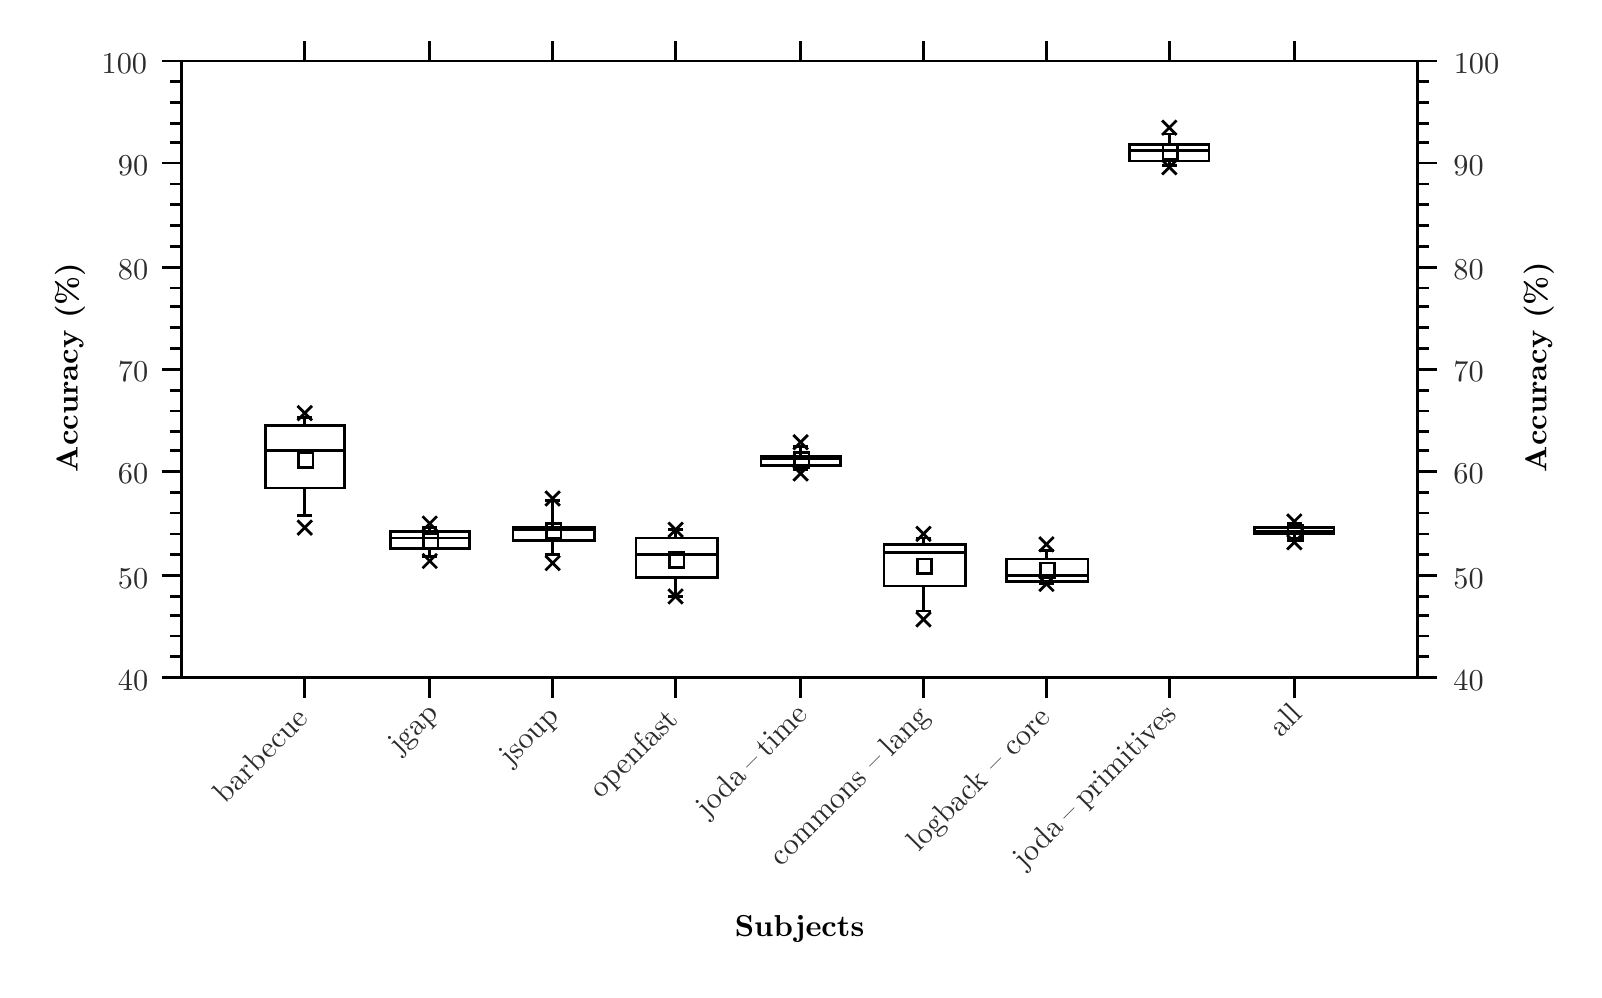
\begin{tikzpicture}{0pt}{0pt}{742pt}{452pt}
	\clip(0pt,452pt) -- (558.587pt,452pt) -- (558.587pt,111.729pt) -- (0pt,111.729pt) -- (0pt,452pt);
\begin{scope}
	\clip(55.7081pt,439.955pt) -- (502.126pt,439.955pt) -- (502.126pt,217.123pt) -- (55.7081pt,217.123pt) -- (55.7081pt,439.955pt);
	\color[rgb]{0,0,0}
	\draw[line width=1pt, line join=miter, line cap=rect](85.8206pt,308.213pt) -- (114.427pt,308.213pt) -- (114.427pt,285.628pt) -- (85.8206pt,285.628pt) -- (85.8206pt,308.213pt);
	\color[rgb]{0,0,0}
	\draw[line width=1pt, line join=miter, line cap=rect](97.8656pt,275.842pt) -- (102.382pt,275.842pt);
	\draw[line width=1pt, line join=miter, line cap=rect](97.8656pt,311.224pt) -- (102.382pt,311.224pt);
	\draw[line width=1pt, line join=miter, line cap=rect](100.124pt,311.224pt) -- (100.124pt,308.213pt);
	\draw[line width=1pt, line join=miter, line cap=rect](100.124pt,275.842pt) -- (100.124pt,285.628pt);
	\draw[line width=1pt, line join=miter, line cap=rect](85.8206pt,299.179pt) -- (114.427pt,299.179pt);
	\draw[line width=1pt, line join=miter, line cap=rect](97.8656pt,273.583pt) -- (102.382pt,269.067pt);
	\draw[line width=1pt, line join=miter, line cap=rect](97.8656pt,269.067pt) -- (102.382pt,273.583pt);
	\draw[line width=1pt, line join=miter, line cap=rect](97.8656pt,314.988pt) -- (102.382pt,310.471pt);
	\draw[line width=1pt, line join=miter, line cap=rect](97.8656pt,310.471pt) -- (102.382pt,314.988pt);
	\draw[line width=1pt, line join=miter, line cap=rect](97.8656pt,298.426pt) -- (103.135pt,298.426pt) -- (103.135pt,293.157pt) -- (97.8656pt,293.157pt) -- (97.8656pt,298.426pt);
	\draw[line width=1pt, line join=miter, line cap=rect](130.989pt,269.819pt) -- (159.596pt,269.819pt) -- (159.596pt,263.797pt) -- (130.989pt,263.797pt) -- (130.989pt,269.819pt);
	\draw[line width=1pt, line join=miter, line cap=rect](143.034pt,260.786pt) -- (147.551pt,260.786pt);
	\draw[line width=1pt, line join=miter, line cap=rect](143.034pt,271.325pt) -- (147.551pt,271.325pt);
	\draw[line width=1pt, line join=miter, line cap=rect](145.293pt,271.325pt) -- (145.293pt,269.819pt);
	\draw[line width=1pt, line join=miter, line cap=rect](145.293pt,260.786pt) -- (145.293pt,263.797pt);
	\draw[line width=1pt, line join=miter, line cap=rect](130.989pt,267.561pt) -- (159.596pt,267.561pt);
	\draw[line width=1pt, line join=miter, line cap=rect](143.034pt,261.538pt) -- (147.551pt,257.022pt);
	\draw[line width=1pt, line join=miter, line cap=rect](143.034pt,257.022pt) -- (147.551pt,261.538pt);
	\draw[line width=1pt, line join=miter, line cap=rect](143.034pt,275.089pt) -- (147.551pt,270.572pt);
	\draw[line width=1pt, line join=miter, line cap=rect](143.034pt,270.572pt) -- (147.551pt,275.089pt);
	\draw[line width=1pt, line join=miter, line cap=rect](143.034pt,269.067pt) -- (148.304pt,269.067pt) -- (148.304pt,263.797pt) -- (143.034pt,263.797pt) -- (143.034pt,269.067pt);
	\draw[line width=1pt, line join=miter, line cap=rect](175.405pt,271.325pt) -- (204.765pt,271.325pt) -- (204.765pt,266.808pt) -- (175.405pt,266.808pt) -- (175.405pt,271.325pt);
	\draw[line width=1pt, line join=miter, line cap=rect](187.45pt,261.538pt) -- (191.967pt,261.538pt);
	\draw[line width=1pt, line join=miter, line cap=rect](187.45pt,281.112pt) -- (191.967pt,281.112pt);
	\draw[line width=1pt, line join=miter, line cap=rect](189.709pt,281.112pt) -- (189.709pt,271.325pt);
	\draw[line width=1pt, line join=miter, line cap=rect](189.709pt,261.538pt) -- (189.709pt,266.808pt);
	\draw[line width=1pt, line join=miter, line cap=rect](175.405pt,270.572pt) -- (204.012pt,270.572pt);
	\draw[line width=1pt, line join=miter, line cap=rect](187.45pt,260.786pt) -- (191.967pt,256.269pt);
	\draw[line width=1pt, line join=miter, line cap=rect](187.45pt,256.269pt) -- (191.967pt,260.786pt);
	\draw[line width=1pt, line join=miter, line cap=rect](187.45pt,284.123pt) -- (191.967pt,279.606pt);
	\draw[line width=1pt, line join=miter, line cap=rect](187.45pt,279.606pt) -- (191.967pt,284.123pt);
	\draw[line width=1pt, line join=miter, line cap=rect](187.45pt,272.831pt) -- (192.72pt,272.831pt) -- (192.72pt,267.561pt) -- (187.45pt,267.561pt) -- (187.45pt,272.831pt);
	\draw[line width=1pt, line join=miter, line cap=rect](219.821pt,267.561pt) -- (249.181pt,267.561pt) -- (249.181pt,253.257pt) -- (219.821pt,253.257pt) -- (219.821pt,267.561pt);
	\draw[line width=1pt, line join=miter, line cap=rect](231.866pt,246.482pt) -- (236.383pt,246.482pt);
	\draw[line width=1pt, line join=miter, line cap=rect](231.866pt,270.572pt) -- (236.383pt,270.572pt);
	\draw[line width=1pt, line join=miter, line cap=rect](234.125pt,270.572pt) -- (234.125pt,267.561pt);
	\draw[line width=1pt, line join=miter, line cap=rect](234.125pt,246.482pt) -- (234.125pt,253.257pt);
	\draw[line width=1pt, line join=miter, line cap=rect](219.821pt,261.538pt) -- (248.428pt,261.538pt);
	\draw[line width=1pt, line join=miter, line cap=rect](231.866pt,248.741pt) -- (236.383pt,244.224pt);
	\draw[line width=1pt, line join=miter, line cap=rect](231.866pt,244.224pt) -- (236.383pt,248.741pt);
	\draw[line width=1pt, line join=miter, line cap=rect](231.866pt,272.831pt) -- (236.383pt,268.314pt);
	\draw[line width=1pt, line join=miter, line cap=rect](231.866pt,268.314pt) -- (236.383pt,272.831pt);
	\draw[line width=1pt, line join=miter, line cap=rect](231.866pt,262.291pt) -- (237.136pt,262.291pt) -- (237.136pt,257.022pt) -- (231.866pt,257.022pt) -- (231.866pt,262.291pt);
	\draw[line width=1pt, line join=miter, line cap=rect](264.99pt,296.921pt) -- (293.597pt,296.921pt) -- (293.597pt,293.909pt) -- (264.99pt,293.909pt) -- (264.99pt,296.921pt);
	\draw[line width=1pt, line join=miter, line cap=rect](277.035pt,292.404pt) -- (281.552pt,292.404pt);
	\draw[line width=1pt, line join=miter, line cap=rect](277.035pt,300.685pt) -- (281.552pt,300.685pt);
	\draw[line width=1pt, line join=miter, line cap=rect](279.293pt,300.685pt) -- (279.293pt,296.921pt);
	\draw[line width=1pt, line join=miter, line cap=rect](279.293pt,292.404pt) -- (279.293pt,293.909pt);
	\draw[line width=1pt, line join=miter, line cap=rect](264.99pt,296.168pt) -- (293.597pt,296.168pt);
	\draw[line width=1pt, line join=miter, line cap=rect](277.035pt,293.157pt) -- (281.552pt,288.64pt);
	\draw[line width=1pt, line join=miter, line cap=rect](277.035pt,288.64pt) -- (281.552pt,293.157pt);
	\draw[line width=1pt, line join=miter, line cap=rect](277.035pt,304.449pt) -- (281.552pt,299.932pt);
	\draw[line width=1pt, line join=miter, line cap=rect](277.035pt,299.932pt) -- (281.552pt,304.449pt);
	\draw[line width=1pt, line join=miter, line cap=rect](277.035pt,298.426pt) -- (282.305pt,298.426pt) -- (282.305pt,293.157pt) -- (277.035pt,293.157pt) -- (277.035pt,298.426pt);
	\draw[line width=1pt, line join=miter, line cap=rect](309.406pt,265.303pt) -- (338.766pt,265.303pt) -- (338.766pt,250.246pt) -- (309.406pt,250.246pt) -- (309.406pt,265.303pt);
	\draw[line width=1pt, line join=miter, line cap=rect](321.451pt,241.213pt) -- (325.968pt,241.213pt);
	\draw[line width=1pt, line join=miter, line cap=rect](321.451pt,267.561pt) -- (325.968pt,267.561pt);
	\draw[line width=1pt, line join=miter, line cap=rect](323.709pt,267.561pt) -- (323.709pt,265.303pt);
	\draw[line width=1pt, line join=miter, line cap=rect](323.709pt,241.213pt) -- (323.709pt,250.246pt);
	\draw[line width=1pt, line join=miter, line cap=rect](309.406pt,262.291pt) -- (338.013pt,262.291pt);
	\draw[line width=1pt, line join=miter, line cap=rect](321.451pt,240.46pt) -- (325.968pt,235.943pt);
	\draw[line width=1pt, line join=miter, line cap=rect](321.451pt,235.943pt) -- (325.968pt,240.46pt);
	\draw[line width=1pt, line join=miter, line cap=rect](321.451pt,271.325pt) -- (325.968pt,266.808pt);
	\draw[line width=1pt, line join=miter, line cap=rect](321.451pt,266.808pt) -- (325.968pt,271.325pt);
	\draw[line width=1pt, line join=miter, line cap=rect](321.451pt,260.033pt) -- (326.721pt,260.033pt) -- (326.721pt,254.763pt) -- (321.451pt,254.763pt) -- (321.451pt,260.033pt);
	\draw[line width=1pt, line join=miter, line cap=rect](353.822pt,260.033pt) -- (383.182pt,260.033pt) -- (383.182pt,251.752pt) -- (353.822pt,251.752pt) -- (353.822pt,260.033pt);
	\draw[line width=1pt, line join=miter, line cap=rect](365.867pt,250.999pt) -- (370.384pt,250.999pt);
	\draw[line width=1pt, line join=miter, line cap=rect](365.867pt,263.044pt) -- (370.384pt,263.044pt);
	\draw[line width=1pt, line join=miter, line cap=rect](368.125pt,263.044pt) -- (368.125pt,260.033pt);
	\draw[line width=1pt, line join=miter, line cap=rect](368.125pt,250.999pt) -- (368.125pt,251.752pt);
	\draw[line width=1pt, line join=miter, line cap=rect](353.822pt,254.01pt) -- (382.429pt,254.01pt);
	\draw[line width=1pt, line join=miter, line cap=rect](365.867pt,253.257pt) -- (370.384pt,248.741pt);
	\draw[line width=1pt, line join=miter, line cap=rect](365.867pt,248.741pt) -- (370.384pt,253.257pt);
	\draw[line width=1pt, line join=miter, line cap=rect](365.867pt,267.561pt) -- (370.384pt,263.044pt);
	\draw[line width=1pt, line join=miter, line cap=rect](365.867pt,263.044pt) -- (370.384pt,267.561pt);
	\draw[line width=1pt, line join=miter, line cap=rect](365.867pt,258.527pt) -- (371.137pt,258.527pt) -- (371.137pt,253.257pt) -- (365.867pt,253.257pt) -- (365.867pt,258.527pt);
	\draw[line width=1pt, line join=miter, line cap=rect](398.238pt,409.842pt) -- (426.845pt,409.842pt) -- (426.845pt,403.82pt) -- (398.238pt,403.82pt) -- (398.238pt,409.842pt);
	\draw[line width=1pt, line join=miter, line cap=rect](410.283pt,402.314pt) -- (414.8pt,402.314pt);
	\draw[line width=1pt, line join=miter, line cap=rect](410.283pt,413.607pt) -- (414.8pt,413.607pt);
	\draw[line width=1pt, line join=miter, line cap=rect](412.541pt,413.607pt) -- (412.541pt,409.842pt);
	\draw[line width=1pt, line join=miter, line cap=rect](412.541pt,402.314pt) -- (412.541pt,403.82pt);
	\draw[line width=1pt, line join=miter, line cap=rect](398.238pt,407.584pt) -- (426.845pt,407.584pt);
	\draw[line width=1pt, line join=miter, line cap=rect](410.283pt,403.82pt) -- (414.8pt,399.303pt);
	\draw[line width=1pt, line join=miter, line cap=rect](410.283pt,399.303pt) -- (414.8pt,403.82pt);
	\draw[line width=1pt, line join=miter, line cap=rect](410.283pt,418.123pt) -- (414.8pt,413.607pt);
	\draw[line width=1pt, line join=miter, line cap=rect](410.283pt,413.607pt) -- (414.8pt,418.123pt);
	\draw[line width=1pt, line join=miter, line cap=rect](410.283pt,409.842pt) -- (415.553pt,409.842pt) -- (415.553pt,404.573pt) -- (410.283pt,404.573pt) -- (410.283pt,409.842pt);
	\draw[line width=1pt, line join=miter, line cap=rect](443.407pt,271.325pt) -- (472.013pt,271.325pt) -- (472.013pt,269.067pt) -- (443.407pt,269.067pt) -- (443.407pt,271.325pt);
	\draw[line width=1pt, line join=miter, line cap=rect](455.452pt,267.561pt) -- (459.968pt,267.561pt);
	\draw[line width=1pt, line join=miter, line cap=rect](455.452pt,272.831pt) -- (459.968pt,272.831pt);
	\draw[line width=1pt, line join=miter, line cap=rect](457.71pt,272.831pt) -- (457.71pt,271.325pt);
	\draw[line width=1pt, line join=miter, line cap=rect](457.71pt,267.561pt) -- (457.71pt,269.067pt);
	\draw[line width=1pt, line join=miter, line cap=rect](443.407pt,269.819pt) -- (472.013pt,269.819pt);
	\draw[line width=1pt, line join=miter, line cap=rect](455.452pt,268.314pt) -- (459.968pt,263.797pt);
	\draw[line width=1pt, line join=miter, line cap=rect](455.452pt,263.797pt) -- (459.968pt,268.314pt);
	\draw[line width=1pt, line join=miter, line cap=rect](455.452pt,275.842pt) -- (459.968pt,271.325pt);
	\draw[line width=1pt, line join=miter, line cap=rect](455.452pt,271.325pt) -- (459.968pt,275.842pt);
	\draw[line width=1pt, line join=miter, line cap=rect](455.452pt,272.078pt) -- (460.721pt,272.078pt) -- (460.721pt,266.808pt) -- (455.452pt,266.808pt) -- (455.452pt,272.078pt);
\end{scope}
\begin{scope}
	\color[rgb]{0,0,0}
	\pgftext[center, base, at={\pgfpoint{18.0675pt}{329.292pt}},rotate=90]{\fontsize{11}{0}\selectfont{\textbf{Accuracy (\%)}}}
	\color[rgb]{0.172549,0.172549,0.172549}
	\pgftext[center, base, at={\pgfpoint{38.1111pt}{212.606pt}}]{\fontsize{11}{0}\selectfont{40}}
	\pgftext[center, base, at={\pgfpoint{38.1111pt}{249.493pt}}]{\fontsize{11}{0}\selectfont{50}}
	\pgftext[center, base, at={\pgfpoint{38.1111pt}{287.134pt}}]{\fontsize{11}{0}\selectfont{60}}
	\pgftext[center, base, at={\pgfpoint{38.1111pt}{324.022pt}}]{\fontsize{11}{0}\selectfont{70}}
	\pgftext[center, base, at={\pgfpoint{38.1111pt}{360.91pt}}]{\fontsize{11}{0}\selectfont{80}}
	\pgftext[center, base, at={\pgfpoint{38.1111pt}{398.55pt}}]{\fontsize{11}{0}\selectfont{90}}
	\pgftext[center, base, at={\pgfpoint{34.9587pt}{435.438pt}}]{\fontsize{11}{0}\selectfont{100}}
	\color[rgb]{0,0,0}
	\draw[line width=1pt, line join=bevel, line cap=rect](55.7081pt,224.651pt) -- (51.9441pt,224.651pt);
	\draw[line width=1pt, line join=bevel, line cap=rect](55.7081pt,232.179pt) -- (51.9441pt,232.179pt);
	\draw[line width=1pt, line join=bevel, line cap=rect](55.7081pt,239.707pt) -- (51.9441pt,239.707pt);
	\draw[line width=1pt, line join=bevel, line cap=rect](55.7081pt,246.482pt) -- (51.9441pt,246.482pt);
	\draw[line width=1pt, line join=bevel, line cap=rect](55.7081pt,261.538pt) -- (51.9441pt,261.538pt);
	\draw[line width=1pt, line join=bevel, line cap=rect](55.7081pt,269.067pt) -- (51.9441pt,269.067pt);
	\draw[line width=1pt, line join=bevel, line cap=rect](55.7081pt,276.595pt) -- (51.9441pt,276.595pt);
	\draw[line width=1pt, line join=bevel, line cap=rect](55.7081pt,284.123pt) -- (51.9441pt,284.123pt);
	\draw[line width=1pt, line join=bevel, line cap=rect](55.7081pt,299.179pt) -- (51.9441pt,299.179pt);
	\draw[line width=1pt, line join=bevel, line cap=rect](55.7081pt,305.954pt) -- (51.9441pt,305.954pt);
	\draw[line width=1pt, line join=bevel, line cap=rect](55.7081pt,313.482pt) -- (51.9441pt,313.482pt);
	\draw[line width=1pt, line join=bevel, line cap=rect](55.7081pt,321.011pt) -- (51.9441pt,321.011pt);
	\draw[line width=1pt, line join=bevel, line cap=rect](55.7081pt,336.067pt) -- (51.9441pt,336.067pt);
	\draw[line width=1pt, line join=bevel, line cap=rect](55.7081pt,343.595pt) -- (51.9441pt,343.595pt);
	\draw[line width=1pt, line join=bevel, line cap=rect](55.7081pt,351.123pt) -- (51.9441pt,351.123pt);
	\draw[line width=1pt, line join=bevel, line cap=rect](55.7081pt,357.898pt) -- (51.9441pt,357.898pt);
	\draw[line width=1pt, line join=bevel, line cap=rect](55.7081pt,372.955pt) -- (51.9441pt,372.955pt);
	\draw[line width=1pt, line join=bevel, line cap=rect](55.7081pt,380.483pt) -- (51.9441pt,380.483pt);
	\draw[line width=1pt, line join=bevel, line cap=rect](55.7081pt,388.011pt) -- (51.9441pt,388.011pt);
	\draw[line width=1pt, line join=bevel, line cap=rect](55.7081pt,395.539pt) -- (51.9441pt,395.539pt);
	\draw[line width=1pt, line join=bevel, line cap=rect](55.7081pt,410.595pt) -- (51.9441pt,410.595pt);
	\draw[line width=1pt, line join=bevel, line cap=rect](55.7081pt,417.371pt) -- (51.9441pt,417.371pt);
	\draw[line width=1pt, line join=bevel, line cap=rect](55.7081pt,424.899pt) -- (51.9441pt,424.899pt);
	\draw[line width=1pt, line join=bevel, line cap=rect](55.7081pt,432.427pt) -- (51.9441pt,432.427pt);
	\draw[line width=1pt, line join=bevel, line cap=rect](55.7081pt,217.123pt) -- (48.9328pt,217.123pt);
	\draw[line width=1pt, line join=bevel, line cap=rect](55.7081pt,254.01pt) -- (48.9328pt,254.01pt);
	\draw[line width=1pt, line join=bevel, line cap=rect](55.7081pt,291.651pt) -- (48.9328pt,291.651pt);
	\draw[line width=1pt, line join=bevel, line cap=rect](55.7081pt,328.539pt) -- (48.9328pt,328.539pt);
	\draw[line width=1pt, line join=bevel, line cap=rect](55.7081pt,365.427pt) -- (48.9328pt,365.427pt);
	\draw[line width=1pt, line join=bevel, line cap=rect](55.7081pt,403.067pt) -- (48.9328pt,403.067pt);
	\draw[line width=1pt, line join=bevel, line cap=rect](55.7081pt,439.955pt) -- (48.9328pt,439.955pt);
	\draw[line width=1pt, line join=bevel, line cap=rect](55.7081pt,439.955pt) -- (55.7081pt,217.123pt);
	\pgftext[center, base, at={\pgfpoint{548.8pt}{329.292pt}},rotate=90]{\fontsize{11}{0}\selectfont{\textbf{Accuracy (\%)}}}
	\color[rgb]{0.172549,0.172549,0.172549}
	\pgftext[center, base, at={\pgfpoint{520.664pt}{212.606pt}}]{\fontsize{11}{0}\selectfont{40}}
	\pgftext[center, base, at={\pgfpoint{520.664pt}{249.493pt}}]{\fontsize{11}{0}\selectfont{50}}
	\pgftext[center, base, at={\pgfpoint{520.664pt}{287.134pt}}]{\fontsize{11}{0}\selectfont{60}}
	\pgftext[center, base, at={\pgfpoint{520.664pt}{324.022pt}}]{\fontsize{11}{0}\selectfont{70}}
	\pgftext[center, base, at={\pgfpoint{520.664pt}{360.91pt}}]{\fontsize{11}{0}\selectfont{80}}
	\pgftext[center, base, at={\pgfpoint{520.664pt}{398.55pt}}]{\fontsize{11}{0}\selectfont{90}}
	\pgftext[center, base, at={\pgfpoint{523.534pt}{435.438pt}}]{\fontsize{11}{0}\selectfont{100}}
	\color[rgb]{0,0,0}
	\draw[line width=1pt, line join=bevel, line cap=rect](502.126pt,224.651pt) -- (505.89pt,224.651pt);
	\draw[line width=1pt, line join=bevel, line cap=rect](502.126pt,232.179pt) -- (505.89pt,232.179pt);
	\draw[line width=1pt, line join=bevel, line cap=rect](502.126pt,239.707pt) -- (505.89pt,239.707pt);
	\draw[line width=1pt, line join=bevel, line cap=rect](502.126pt,246.482pt) -- (505.89pt,246.482pt);
	\draw[line width=1pt, line join=bevel, line cap=rect](502.126pt,261.538pt) -- (505.89pt,261.538pt);
	\draw[line width=1pt, line join=bevel, line cap=rect](502.126pt,269.067pt) -- (505.89pt,269.067pt);
	\draw[line width=1pt, line join=bevel, line cap=rect](502.126pt,276.595pt) -- (505.89pt,276.595pt);
	\draw[line width=1pt, line join=bevel, line cap=rect](502.126pt,284.123pt) -- (505.89pt,284.123pt);
	\draw[line width=1pt, line join=bevel, line cap=rect](502.126pt,299.179pt) -- (505.89pt,299.179pt);
	\draw[line width=1pt, line join=bevel, line cap=rect](502.126pt,305.954pt) -- (505.89pt,305.954pt);
	\draw[line width=1pt, line join=bevel, line cap=rect](502.126pt,313.482pt) -- (505.89pt,313.482pt);
	\draw[line width=1pt, line join=bevel, line cap=rect](502.126pt,321.011pt) -- (505.89pt,321.011pt);
	\draw[line width=1pt, line join=bevel, line cap=rect](502.126pt,336.067pt) -- (505.89pt,336.067pt);
	\draw[line width=1pt, line join=bevel, line cap=rect](502.126pt,343.595pt) -- (505.89pt,343.595pt);
	\draw[line width=1pt, line join=bevel, line cap=rect](502.126pt,351.123pt) -- (505.89pt,351.123pt);
	\draw[line width=1pt, line join=bevel, line cap=rect](502.126pt,357.898pt) -- (505.89pt,357.898pt);
	\draw[line width=1pt, line join=bevel, line cap=rect](502.126pt,372.955pt) -- (505.89pt,372.955pt);
	\draw[line width=1pt, line join=bevel, line cap=rect](502.126pt,380.483pt) -- (505.89pt,380.483pt);
	\draw[line width=1pt, line join=bevel, line cap=rect](502.126pt,388.011pt) -- (505.89pt,388.011pt);
	\draw[line width=1pt, line join=bevel, line cap=rect](502.126pt,395.539pt) -- (505.89pt,395.539pt);
	\draw[line width=1pt, line join=bevel, line cap=rect](502.126pt,410.595pt) -- (505.89pt,410.595pt);
	\draw[line width=1pt, line join=bevel, line cap=rect](502.126pt,417.371pt) -- (505.89pt,417.371pt);
	\draw[line width=1pt, line join=bevel, line cap=rect](502.126pt,424.899pt) -- (505.89pt,424.899pt);
	\draw[line width=1pt, line join=bevel, line cap=rect](502.126pt,432.427pt) -- (505.89pt,432.427pt);
	\draw[line width=1pt, line join=bevel, line cap=rect](502.126pt,217.123pt) -- (508.901pt,217.123pt);
	\draw[line width=1pt, line join=bevel, line cap=rect](502.126pt,254.01pt) -- (508.901pt,254.01pt);
	\draw[line width=1pt, line join=bevel, line cap=rect](502.126pt,291.651pt) -- (508.901pt,291.651pt);
	\draw[line width=1pt, line join=bevel, line cap=rect](502.126pt,328.539pt) -- (508.901pt,328.539pt);
	\draw[line width=1pt, line join=bevel, line cap=rect](502.126pt,365.427pt) -- (508.901pt,365.427pt);
	\draw[line width=1pt, line join=bevel, line cap=rect](502.126pt,403.067pt) -- (508.901pt,403.067pt);
	\draw[line width=1pt, line join=bevel, line cap=rect](502.126pt,439.955pt) -- (508.901pt,439.955pt);
	\draw[line width=1pt, line join=bevel, line cap=rect](502.126pt,439.955pt) -- (502.126pt,217.123pt);
	\pgftext[center, base, at={\pgfpoint{278.917pt}{123.774pt}}]{\fontsize{11}{0}\selectfont{\textbf{Subjects}}}
	\color[rgb]{0.172549,0.172549,0.172549}
	\pgftext[center, base, at={\pgfpoint{86.5666pt}{186.638pt}},rotate=45]{\fontsize{11}{0}\selectfont{barbecue}}
	\pgftext[center, base, at={\pgfpoint{141.542pt}{196.444pt}},rotate=45]{\fontsize{11}{0}\selectfont{jgap}}
	\pgftext[center, base, at={\pgfpoint{183.4pt}{193.886pt}},rotate=45]{\fontsize{11}{0}\selectfont{jsoup}}
	\pgftext[center, base, at={\pgfpoint{221.245pt}{187.316pt}},rotate=45]{\fontsize{11}{0}\selectfont{openfast}}
	\pgftext[center, base, at={\pgfpoint{252.794pt}{173.696pt}},rotate=45]{\fontsize{11}{0}\selectfont{joda}}
	\pgftext[center, base, at={\pgfpoint{263.706pt}{184.608pt}},rotate=45]{\fontsize{11}{0}\selectfont{--}}
	\pgftext[center, base, at={\pgfpoint{274.706pt}{195.608pt}},rotate=45]{\fontsize{11}{0}\selectfont{time}}
	\pgftext[center, base, at={\pgfpoint{287.936pt}{164.422pt}},rotate=45]{\fontsize{11}{0}\selectfont{commons}}
	\pgftext[center, base, at={\pgfpoint{308.206pt}{184.692pt}},rotate=45]{\fontsize{11}{0}\selectfont{--}}
	\pgftext[center, base, at={\pgfpoint{319.068pt}{195.554pt}},rotate=45]{\fontsize{11}{0}\selectfont{lang}}
	\pgftext[center, base, at={\pgfpoint{334.627pt}{166.697pt}},rotate=45]{\fontsize{11}{0}\selectfont{logback}}
	\pgftext[center, base, at={\pgfpoint{351.848pt}{183.918pt}},rotate=45]{\fontsize{11}{0}\selectfont{--}}
	\pgftext[center, base, at={\pgfpoint{363.072pt}{195.142pt}},rotate=45]{\fontsize{11}{0}\selectfont{core}}
	\pgftext[center, base, at={\pgfpoint{367.411pt}{155.065pt}},rotate=45]{\fontsize{11}{0}\selectfont{joda}}
	\pgftext[center, base, at={\pgfpoint{378.323pt}{165.977pt}},rotate=45]{\fontsize{11}{0}\selectfont{--}}
	\pgftext[center, base, at={\pgfpoint{398.826pt}{186.48pt}},rotate=45]{\fontsize{11}{0}\selectfont{primitives}}
	\pgftext[center, base, at={\pgfpoint{456.857pt}{199.343pt}},rotate=45]{\fontsize{11}{0}\selectfont{all}}
	\color[rgb]{0,0,0}
	\draw[line width=1pt, line join=bevel, line cap=rect](100.124pt,217.123pt) -- (100.124pt,210.347pt);
	\draw[line width=1pt, line join=bevel, line cap=rect](145.293pt,217.123pt) -- (145.293pt,210.347pt);
	\draw[line width=1pt, line join=bevel, line cap=rect](189.709pt,217.123pt) -- (189.709pt,210.347pt);
	\draw[line width=1pt, line join=bevel, line cap=rect](234.125pt,217.123pt) -- (234.125pt,210.347pt);
	\draw[line width=1pt, line join=bevel, line cap=rect](279.293pt,217.123pt) -- (279.293pt,210.347pt);
	\draw[line width=1pt, line join=bevel, line cap=rect](323.709pt,217.123pt) -- (323.709pt,210.347pt);
	\draw[line width=1pt, line join=bevel, line cap=rect](368.125pt,217.123pt) -- (368.125pt,210.347pt);
	\draw[line width=1pt, line join=bevel, line cap=rect](412.541pt,217.123pt) -- (412.541pt,210.347pt);
	\draw[line width=1pt, line join=bevel, line cap=rect](457.71pt,217.123pt) -- (457.71pt,210.347pt);
	\draw[line width=1pt, line join=bevel, line cap=rect](55.7081pt,217.123pt) -- (502.126pt,217.123pt);
	\draw[line width=1pt, line join=bevel, line cap=rect](100.124pt,439.955pt) -- (100.124pt,446.73pt);
	\draw[line width=1pt, line join=bevel, line cap=rect](145.293pt,439.955pt) -- (145.293pt,446.73pt);
	\draw[line width=1pt, line join=bevel, line cap=rect](189.709pt,439.955pt) -- (189.709pt,446.73pt);
	\draw[line width=1pt, line join=bevel, line cap=rect](234.125pt,439.955pt) -- (234.125pt,446.73pt);
	\draw[line width=1pt, line join=bevel, line cap=rect](279.293pt,439.955pt) -- (279.293pt,446.73pt);
	\draw[line width=1pt, line join=bevel, line cap=rect](323.709pt,439.955pt) -- (323.709pt,446.73pt);
	\draw[line width=1pt, line join=bevel, line cap=rect](368.125pt,439.955pt) -- (368.125pt,446.73pt);
	\draw[line width=1pt, line join=bevel, line cap=rect](412.541pt,439.955pt) -- (412.541pt,446.73pt);
	\draw[line width=1pt, line join=bevel, line cap=rect](457.71pt,439.955pt) -- (457.71pt,446.73pt);
	\draw[line width=1pt, line join=bevel, line cap=rect](55.7081pt,439.955pt) -- (502.126pt,439.955pt);
\end{scope}
\end{tikzpicture}

  \end{adjustbox}
  \caption{Method-level cross-validation accuracy of each test subject using all feature sets (\ding{172} \ding{173} \ding{174} \ding{175}).}
  \vspace{2mm}
  \hrule
  \label{fig:individual_cross_validation_method_1_2_3_4_graph}
\end{figure}

\begin{table}[!tb]
  \centering
  \rowcolors{1}{gray!30}{gray!20}
  \begin{threeparttable}
    \begin{tabular}{|l|r|r|}
      \rowcolor[RGB]{169,196,223}
      \hline & \textbf{Class-Level} & \textbf{Method-Level} \\
      \hline \cellcolor[RGB]{169,196,223} \textbf{logback-core} & 12 & 138 \\
      \hline \cellcolor[RGB]{169,196,223} \textbf{barbecue} & 2 & 36 \\
      \hline \cellcolor[RGB]{169,196,223} \textbf{jgap} & 27 & 197 \\
      \hline \cellcolor[RGB]{169,196,223} \textbf{commons-lang} & 18 & 132 \\
      \hline \cellcolor[RGB]{169,196,223} \textbf{joda-time} & 21 & 259 \\
      \hline \cellcolor[RGB]{169,196,223} \textbf{openfast} & 24 & 73 \\
      \hline \cellcolor[RGB]{169,196,223} \textbf{jsoup} & 13 & 58 \\
      \hline \cellcolor[RGB]{169,196,223} \textbf{joda-primitives} & 1 & 165 \\
      \hline \cellcolor[RGB]{169,196,223} \textbf{all} & 191 & 1104 \\
      \hline
    \end{tabular}
  \end{threeparttable}
  \caption{The number of data points used for each category based on undersampling the lowest category to provide balanced data, for each test subject.}
  \vspace{2mm}
  \hrule
  \label{tab:experiments_undersampled_data}
\end{table}

We have looked at the overall cross-validation accuracy using the different feature sets and found that using all feature sets provides the best accuracy. To understand how different projects behave when we apply our technique, we considered each test subject independently using all the feature sets. Figure~\ref{fig:individual_cross_validation_class_1_2_3_4_graph} illustrates the class-level cross-validations of each test subjects with the \emph{all} subject as a comparison. We can see that all but \emph{barbecue} and \emph{joda-primitives} are similar with respect to mean accuracy. All of the independent test subjects have larger variation in their accuracies compared to the method-level accuracies, which is most likely due to the limited data that each test subject provides on its own. Recall that we are undersampling our data to achieve balanced categories, thus in some situations the amount of data being used can drastically be reduced. In the case of \emph{barbecue}, the undersampling only allowed two instances of data to be used for each category, which explains the huge variation that it has. \emph{joda-primitives} only had one instance for each category, which resulted in a cross-validation accuracy of 0\%. Table~\ref{tab:experiments_undersampled_data} provides details regarding the number of data points being used with undersampling. Moving on to the method-level source code units presented in Figure~\ref{fig:individual_cross_validation_method_1_2_3_4_graph}, we can see that all but \emph{barbecue}, \emph{joda-primitives}, and \emph{joda-time} are comparable to the \emph{all} accuracy with slightly larger variations. Again, \emph{barbecue} has a low number of data points being used which can explain the larger variations in accuracy. With \emph{joda-primitives}, we have an unusually high cross-validation accuracy. If we look at Figure~\ref{fig:mutation_distributions_method_joda-primitives} in Appendix~\ref{app:mutation_score_distributions}, we can see that the mutation score distribution is cleanly separated according to the category ranges (i.e., a large number of 100\% and 50\% mutation score methods, with the remaining between these values). It might just be the case that the \emph{joda-primitives}'s data is easier to separate with the \gls{svm}, thus allowing it achieve higher accuracy. \emph{joda-time} presents a slightly higher cross-validation accuracy then the other test subjects. This could be because it has the most data points available for the \gls{svm} or because it has 48 methods that are very similar (most likely duplicates) as we saw in the covered mutant distribution (see Figure~\ref{fig:covered_mutant_distributions_method_all}). Similar methods would be classified in the same category, thus this could slightly inflate the cross-validation accuracy if this was the case.


\subsection{Prediction on Unknown Data}
\label{subsec:experiment_prediction}
\begin{quote}
  \emph{\textbf{Research Question:} How well can our approach predict on unknown data, within an individual software system and across software systems?}
\end{quote}

\noindent
By using LIBSVM we want to train a classifier such that it can predict well on \emph{unknown data}. Parameter selection and the training/testing data sets play an important role in developing a good classifier. Ultimately, we want to obtain a classifier that is able to \emph{generalize} to new, unknown data. In our specific case, we have eight different test subjects (that are most likely not similar to each other in terms of features) in which we want to maximize our performance at predicting unknown data. We used cross-validation in Section~\ref{subsec:experiment_cross_validation} as it mitigates the overfitting problem introduced by training (i.e., a model becomes specifically tuned for the training data set)~\cite{HCL03}. Parameter selection also occurred automatically using a grid search approach to find a set of parameters that maximized the cross-validation accuracy on the training data set.

\begin{table}[!tb]
  \centering
  \rowcolors{1}{gray!30}{gray!20}
  \begin{threeparttable}
    \begin{tabular}{|l|>{\raggedleft\arraybackslash}p{4.25cm}|>{\raggedleft\arraybackslash}p{4.25cm}|}
      \rowcolor[RGB]{169,196,223}
      \hline & \textbf{Class-Level\scriptsize\newline[LOW/MEDIUM/HIGH]} & \textbf{Method-Level\scriptsize\newline[LOW/MEDIUM/HIGH]} \\
      \hline \cellcolor[RGB]{169,196,223} \textbf{logback-core} & 36/43/0 & 0/3/30 \\
      \hline \cellcolor[RGB]{169,196,223} \textbf{barbecue} & 13/12/0 & 20/15/0 \\
      \hline \cellcolor[RGB]{169,196,223} \textbf{jgap} & 24/19/0 & 26/0/38 \\
      \hline \cellcolor[RGB]{169,196,223} \textbf{commons-lang} & 0/65/5 & 0/186/207 \\
      \hline \cellcolor[RGB]{169,196,223} \textbf{joda-time} & 0/87/44 & 0/296/946 \\
      \hline \cellcolor[RGB]{169,196,223} \textbf{openfast} & 0/33/15 & 0/69/113 \\
      \hline \cellcolor[RGB]{169,196,223} \textbf{jsoup} & 0/18/26 & 0/50/157 \\
      \hline \cellcolor[RGB]{169,196,223} \textbf{joda-primitives} & 0/64/6 & 0/105/75 \\
      \hline \cellcolor[RGB]{169,196,223} \textbf{all\_but\_logback-core} & 48/55/12 & 138/141/168 \\
      \hline \cellcolor[RGB]{169,196,223} \textbf{all\_but\_barbecue} & 15/14/2 & 56/51/36 \\
      \hline \cellcolor[RGB]{169,196,223} \textbf{all\_but\_jgap} & 51/46/27 & 223/197/235 \\
      \hline \cellcolor[RGB]{169,196,223} \textbf{all\_but\_commons-lang} & 18/83/23 & 132/318/339 \\
      \hline \cellcolor[RGB]{169,196,223} \textbf{all\_but\_joda-time} & 21/108/65 & 256/555/1205 \\
      \hline \cellcolor[RGB]{169,196,223} \textbf{all\_but\_openfast} & 24/57/39 & 73/142/186 \\
      \hline \cellcolor[RGB]{169,196,223} \textbf{all\_but\_jsoup} & 13/31/39 & 58/108/215 \\
      \hline \cellcolor[RGB]{169,196,223} \textbf{all\_but\_joda-primitives} & 1/65/7 & 165/270/240 \\
      \hline
    \end{tabular}
  \end{threeparttable}
  \caption{The number of data points present in each category for each test subject's prediction data set after undersampling (if possible) has occurred.}
  \vspace{2mm}
  \hrule
  \label{tab:experiments_remaining_data}
\end{table}

We conducted a number of tests where we use LIBSVM's \emph{easy script} to find the best parameters that maximize cross-validation accuracy and then apply the classifier to unknown data. We continue to undersample our data and conduct each experiment ten times to determine the prediction accuracy. We are interested in the prediction accuracy of unknown data. To investigate this we can consider the \emph{all\_but\_<subject>} sets, where we train our classifier on all but the \emph{<subject>} and then predict on the excluded test subject. In addition, we consider the individual test subjects where we train using the undersampled data and predict on the remaining unknown data within the individual test subject (i.e., what is left from the undersampling). See Table~\ref{tab:experiments_undersampled_data} for the number of remaining unknown values of the individual test subjects.

\begin{figure}[!tb]
  \centering
  \begin{adjustbox}{max size={.95\textwidth}{.95\textheight}}
    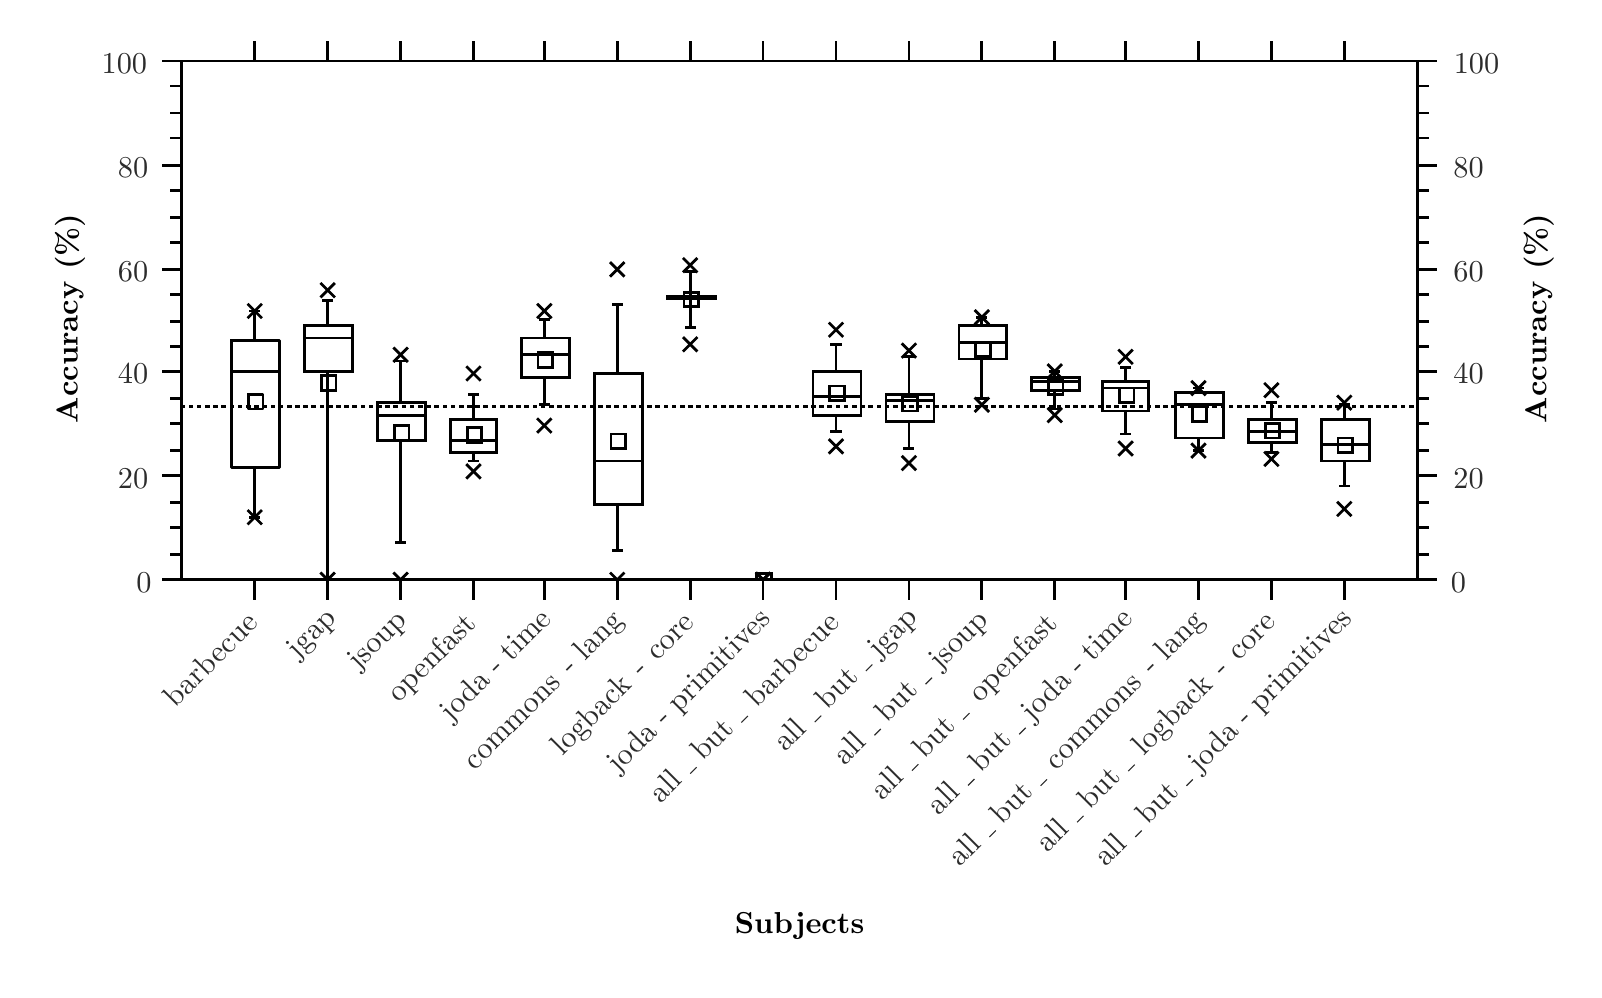
\begin{tikzpicture}{0pt}{0pt}{742pt}{452pt}
	\clip(0pt,452pt) -- (558.587pt,452pt) -- (558.587pt,111.729pt) -- (0pt,111.729pt) -- (0pt,452pt);
\begin{scope}
	\clip(55.7081pt,439.955pt) -- (502.126pt,439.955pt) -- (502.126pt,252.505pt) -- (55.7081pt,252.505pt) -- (55.7081pt,439.955pt);
	\color[rgb]{0,0,0}
	\draw[line width=1pt, line join=bevel, line cap=rect](73.7756pt,339.078pt) -- (91.0903pt,339.078pt) -- (91.0903pt,293.157pt) -- (73.7756pt,293.157pt) -- (73.7756pt,339.078pt);
	\color[rgb]{0,0,0}
	\draw[line width=1pt, line join=bevel, line cap=rect](80.5509pt,275.089pt) -- (83.5622pt,275.089pt);
	\draw[line width=1pt, line join=bevel, line cap=rect](80.5509pt,349.618pt) -- (83.5622pt,349.618pt);
	\draw[line width=1pt, line join=bevel, line cap=rect](82.0566pt,349.618pt) -- (82.0566pt,339.078pt);
	\draw[line width=1pt, line join=bevel, line cap=rect](82.0566pt,275.089pt) -- (82.0566pt,293.157pt);
	\draw[line width=1pt, line join=bevel, line cap=rect](73.7756pt,327.786pt) -- (90.3375pt,327.786pt);
	\draw[line width=1pt, line join=bevel, line cap=rect](79.7981pt,277.347pt) -- (84.315pt,272.831pt);
	\draw[line width=1pt, line join=bevel, line cap=rect](79.7981pt,272.831pt) -- (84.315pt,277.347pt);
	\draw[line width=1pt, line join=bevel, line cap=rect](79.7981pt,351.876pt) -- (84.315pt,347.359pt);
	\draw[line width=1pt, line join=bevel, line cap=rect](79.7981pt,347.359pt) -- (84.315pt,351.876pt);
	\draw[line width=1pt, line join=bevel, line cap=rect](79.7981pt,319.505pt) -- (85.0678pt,319.505pt) -- (85.0678pt,314.235pt) -- (79.7981pt,314.235pt) -- (79.7981pt,319.505pt);
	\draw[line width=1pt, line join=miter, line cap=rect](100.124pt,344.348pt) -- (117.439pt,344.348pt) -- (117.439pt,327.786pt) -- (100.124pt,327.786pt) -- (100.124pt,344.348pt);
	\draw[line width=1pt, line join=miter, line cap=rect](106.899pt,252.505pt) -- (109.911pt,252.505pt);
	\draw[line width=1pt, line join=miter, line cap=rect](106.899pt,353.382pt) -- (109.911pt,353.382pt);
	\draw[line width=1pt, line join=miter, line cap=rect](108.405pt,353.382pt) -- (108.405pt,344.348pt);
	\draw[line width=1pt, line join=miter, line cap=rect](108.405pt,252.505pt) -- (108.405pt,327.786pt);
	\draw[line width=1pt, line join=miter, line cap=rect](100.124pt,339.831pt) -- (116.686pt,339.831pt);
	\draw[line width=1pt, line join=miter, line cap=rect](106.147pt,254.763pt) -- (110.663pt,250.246pt);
	\draw[line width=1pt, line join=miter, line cap=rect](106.147pt,250.246pt) -- (110.663pt,254.763pt);
	\draw[line width=1pt, line join=miter, line cap=rect](106.147pt,359.404pt) -- (110.663pt,354.887pt);
	\draw[line width=1pt, line join=miter, line cap=rect](106.147pt,354.887pt) -- (110.663pt,359.404pt);
	\draw[line width=1pt, line join=miter, line cap=rect](106.147pt,326.28pt) -- (111.416pt,326.28pt) -- (111.416pt,321.011pt) -- (106.147pt,321.011pt) -- (106.147pt,326.28pt);
	\draw[line width=1pt, line join=miter, line cap=rect](126.472pt,316.494pt) -- (143.787pt,316.494pt) -- (143.787pt,302.943pt) -- (126.472pt,302.943pt) -- (126.472pt,316.494pt);
	\draw[line width=1pt, line join=miter, line cap=rect](133.248pt,266.055pt) -- (136.259pt,266.055pt);
	\draw[line width=1pt, line join=miter, line cap=rect](133.248pt,331.55pt) -- (136.259pt,331.55pt);
	\draw[line width=1pt, line join=miter, line cap=rect](134.753pt,331.55pt) -- (134.753pt,316.494pt);
	\draw[line width=1pt, line join=miter, line cap=rect](134.753pt,266.055pt) -- (134.753pt,302.943pt);
	\draw[line width=1pt, line join=miter, line cap=rect](126.472pt,311.977pt) -- (143.034pt,311.977pt);
	\draw[line width=1pt, line join=miter, line cap=rect](132.495pt,254.763pt) -- (137.012pt,250.246pt);
	\draw[line width=1pt, line join=miter, line cap=rect](132.495pt,250.246pt) -- (137.012pt,254.763pt);
	\draw[line width=1pt, line join=miter, line cap=rect](132.495pt,336.067pt) -- (137.012pt,331.55pt);
	\draw[line width=1pt, line join=miter, line cap=rect](132.495pt,331.55pt) -- (137.012pt,336.067pt);
	\draw[line width=1pt, line join=miter, line cap=rect](132.495pt,308.213pt) -- (137.765pt,308.213pt) -- (137.765pt,302.943pt) -- (132.495pt,302.943pt) -- (132.495pt,308.213pt);
	\draw[line width=1pt, line join=miter, line cap=rect](152.821pt,310.471pt) -- (169.383pt,310.471pt) -- (169.383pt,298.426pt) -- (152.821pt,298.426pt) -- (152.821pt,310.471pt);
	\draw[line width=1pt, line join=miter, line cap=rect](159.596pt,295.415pt) -- (162.607pt,295.415pt);
	\draw[line width=1pt, line join=miter, line cap=rect](159.596pt,319.505pt) -- (162.607pt,319.505pt);
	\draw[line width=1pt, line join=miter, line cap=rect](161.102pt,319.505pt) -- (161.102pt,310.471pt);
	\draw[line width=1pt, line join=miter, line cap=rect](161.102pt,295.415pt) -- (161.102pt,298.426pt);
	\draw[line width=1pt, line join=miter, line cap=rect](152.821pt,302.943pt) -- (169.383pt,302.943pt);
	\draw[line width=1pt, line join=miter, line cap=rect](158.843pt,293.909pt) -- (163.36pt,289.393pt);
	\draw[line width=1pt, line join=miter, line cap=rect](158.843pt,289.393pt) -- (163.36pt,293.909pt);
	\draw[line width=1pt, line join=miter, line cap=rect](158.843pt,329.292pt) -- (163.36pt,324.775pt);
	\draw[line width=1pt, line join=miter, line cap=rect](158.843pt,324.775pt) -- (163.36pt,329.292pt);
	\draw[line width=1pt, line join=miter, line cap=rect](158.843pt,307.46pt) -- (164.113pt,307.46pt) -- (164.113pt,302.19pt) -- (158.843pt,302.19pt) -- (158.843pt,307.46pt);
	\draw[line width=1pt, line join=miter, line cap=rect](178.417pt,339.831pt) -- (195.731pt,339.831pt) -- (195.731pt,325.528pt) -- (178.417pt,325.528pt) -- (178.417pt,339.831pt);
	\draw[line width=1pt, line join=miter, line cap=rect](185.192pt,315.741pt) -- (188.203pt,315.741pt);
	\draw[line width=1pt, line join=miter, line cap=rect](185.192pt,346.606pt) -- (188.203pt,346.606pt);
	\draw[line width=1pt, line join=miter, line cap=rect](186.697pt,346.606pt) -- (186.697pt,339.831pt);
	\draw[line width=1pt, line join=miter, line cap=rect](186.697pt,315.741pt) -- (186.697pt,325.528pt);
	\draw[line width=1pt, line join=miter, line cap=rect](178.417pt,333.808pt) -- (194.978pt,333.808pt);
	\draw[line width=1pt, line join=miter, line cap=rect](184.439pt,310.471pt) -- (188.956pt,305.954pt);
	\draw[line width=1pt, line join=miter, line cap=rect](184.439pt,305.954pt) -- (188.956pt,310.471pt);
	\draw[line width=1pt, line join=miter, line cap=rect](184.439pt,351.876pt) -- (188.956pt,347.359pt);
	\draw[line width=1pt, line join=miter, line cap=rect](184.439pt,347.359pt) -- (188.956pt,351.876pt);
	\draw[line width=1pt, line join=miter, line cap=rect](184.439pt,334.561pt) -- (189.709pt,334.561pt) -- (189.709pt,329.292pt) -- (184.439pt,329.292pt) -- (184.439pt,334.561pt);
	\draw[line width=1pt, line join=miter, line cap=rect](204.765pt,327.033pt) -- (222.08pt,327.033pt) -- (222.08pt,279.606pt) -- (204.765pt,279.606pt) -- (204.765pt,327.033pt);
	\draw[line width=1pt, line join=miter, line cap=rect](211.54pt,263.044pt) -- (214.552pt,263.044pt);
	\draw[line width=1pt, line join=miter, line cap=rect](211.54pt,351.876pt) -- (214.552pt,351.876pt);
	\draw[line width=1pt, line join=miter, line cap=rect](213.046pt,351.876pt) -- (213.046pt,327.033pt);
	\draw[line width=1pt, line join=miter, line cap=rect](213.046pt,263.044pt) -- (213.046pt,279.606pt);
	\draw[line width=1pt, line join=miter, line cap=rect](204.765pt,295.415pt) -- (221.327pt,295.415pt);
	\draw[line width=1pt, line join=miter, line cap=rect](210.787pt,254.763pt) -- (215.304pt,250.246pt);
	\draw[line width=1pt, line join=miter, line cap=rect](210.787pt,250.246pt) -- (215.304pt,254.763pt);
	\draw[line width=1pt, line join=miter, line cap=rect](210.787pt,366.932pt) -- (215.304pt,362.415pt);
	\draw[line width=1pt, line join=miter, line cap=rect](210.787pt,362.415pt) -- (215.304pt,366.932pt);
	\draw[line width=1pt, line join=miter, line cap=rect](210.787pt,305.202pt) -- (216.057pt,305.202pt) -- (216.057pt,299.932pt) -- (210.787pt,299.932pt) -- (210.787pt,305.202pt);
	\draw[line width=1pt, line join=miter, line cap=rect](231.113pt,354.887pt) -- (248.428pt,354.887pt) -- (248.428pt,354.134pt) -- (231.113pt,354.134pt) -- (231.113pt,354.887pt);
	\draw[line width=1pt, line join=miter, line cap=rect](237.889pt,343.595pt) -- (240.9pt,343.595pt);
	\draw[line width=1pt, line join=miter, line cap=rect](237.889pt,363.921pt) -- (240.9pt,363.921pt);
	\draw[line width=1pt, line join=miter, line cap=rect](239.394pt,363.921pt) -- (239.394pt,354.887pt);
	\draw[line width=1pt, line join=miter, line cap=rect](239.394pt,343.595pt) -- (239.394pt,354.134pt);
	\draw[line width=1pt, line join=miter, line cap=rect](231.113pt,354.887pt) -- (247.675pt,354.887pt);
	\draw[line width=1pt, line join=miter, line cap=rect](237.136pt,339.831pt) -- (241.653pt,335.314pt);
	\draw[line width=1pt, line join=miter, line cap=rect](237.136pt,335.314pt) -- (241.653pt,339.831pt);
	\draw[line width=1pt, line join=miter, line cap=rect](237.136pt,368.438pt) -- (241.653pt,363.921pt);
	\draw[line width=1pt, line join=miter, line cap=rect](237.136pt,363.921pt) -- (241.653pt,368.438pt);
	\draw[line width=1pt, line join=miter, line cap=rect](237.136pt,356.393pt) -- (242.406pt,356.393pt) -- (242.406pt,351.123pt) -- (237.136pt,351.123pt) -- (237.136pt,356.393pt);
	\draw[line width=1pt, line join=miter, line cap=rect](257.462pt,252.505pt) -- (274.777pt,252.505pt) -- (274.777pt,251.752pt) -- (257.462pt,251.752pt) -- (257.462pt,252.505pt);
	\draw[line width=1pt, line join=miter, line cap=rect](264.237pt,252.505pt) -- (267.248pt,252.505pt);
	\draw[line width=1pt, line join=miter, line cap=rect](264.237pt,252.505pt) -- (267.248pt,252.505pt);
	\draw[line width=1pt, line join=miter, line cap=rect](257.462pt,252.505pt) -- (274.024pt,252.505pt);
	\draw[line width=1pt, line join=miter, line cap=rect](263.484pt,254.763pt) -- (268.001pt,250.246pt);
	\draw[line width=1pt, line join=miter, line cap=rect](263.484pt,250.246pt) -- (268.001pt,254.763pt);
	\draw[line width=1pt, line join=miter, line cap=rect](263.484pt,254.763pt) -- (268.001pt,250.246pt);
	\draw[line width=1pt, line join=miter, line cap=rect](263.484pt,250.246pt) -- (268.001pt,254.763pt);
	\draw[line width=1pt, line join=miter, line cap=rect](263.484pt,254.763pt) -- (268.754pt,254.763pt) -- (268.754pt,249.493pt) -- (263.484pt,249.493pt) -- (263.484pt,254.763pt);
	\draw[line width=1pt, line join=miter, line cap=rect](283.81pt,327.786pt) -- (301.125pt,327.786pt) -- (301.125pt,311.977pt) -- (283.81pt,311.977pt) -- (283.81pt,327.786pt);
	\draw[line width=1pt, line join=miter, line cap=rect](290.586pt,305.954pt) -- (293.597pt,305.954pt);
	\draw[line width=1pt, line join=miter, line cap=rect](290.586pt,337.572pt) -- (293.597pt,337.572pt);
	\draw[line width=1pt, line join=miter, line cap=rect](292.091pt,337.572pt) -- (292.091pt,327.786pt);
	\draw[line width=1pt, line join=miter, line cap=rect](292.091pt,305.954pt) -- (292.091pt,311.977pt);
	\draw[line width=1pt, line join=miter, line cap=rect](283.81pt,318.752pt) -- (300.372pt,318.752pt);
	\draw[line width=1pt, line join=miter, line cap=rect](289.833pt,302.943pt) -- (294.35pt,298.426pt);
	\draw[line width=1pt, line join=miter, line cap=rect](289.833pt,298.426pt) -- (294.35pt,302.943pt);
	\draw[line width=1pt, line join=miter, line cap=rect](289.833pt,345.101pt) -- (294.35pt,340.584pt);
	\draw[line width=1pt, line join=miter, line cap=rect](289.833pt,340.584pt) -- (294.35pt,345.101pt);
	\draw[line width=1pt, line join=miter, line cap=rect](289.833pt,322.516pt) -- (295.103pt,322.516pt) -- (295.103pt,317.247pt) -- (289.833pt,317.247pt) -- (289.833pt,322.516pt);
	\draw[line width=1pt, line join=miter, line cap=rect](310.159pt,319.505pt) -- (327.473pt,319.505pt) -- (327.473pt,309.718pt) -- (310.159pt,309.718pt) -- (310.159pt,319.505pt);
	\draw[line width=1pt, line join=miter, line cap=rect](316.934pt,299.932pt) -- (319.945pt,299.932pt);
	\draw[line width=1pt, line join=miter, line cap=rect](316.934pt,333.056pt) -- (319.945pt,333.056pt);
	\draw[line width=1pt, line join=miter, line cap=rect](318.44pt,333.056pt) -- (318.44pt,319.505pt);
	\draw[line width=1pt, line join=miter, line cap=rect](318.44pt,299.932pt) -- (318.44pt,309.718pt);
	\draw[line width=1pt, line join=miter, line cap=rect](310.159pt,317.247pt) -- (326.721pt,317.247pt);
	\draw[line width=1pt, line join=miter, line cap=rect](316.181pt,296.921pt) -- (320.698pt,292.404pt);
	\draw[line width=1pt, line join=miter, line cap=rect](316.181pt,292.404pt) -- (320.698pt,296.921pt);
	\draw[line width=1pt, line join=miter, line cap=rect](316.181pt,337.572pt) -- (320.698pt,333.056pt);
	\draw[line width=1pt, line join=miter, line cap=rect](316.181pt,333.056pt) -- (320.698pt,337.572pt);
	\draw[line width=1pt, line join=miter, line cap=rect](316.181pt,318.752pt) -- (321.451pt,318.752pt) -- (321.451pt,313.482pt) -- (316.181pt,313.482pt) -- (316.181pt,318.752pt);
	\draw[line width=1pt, line join=miter, line cap=rect](336.507pt,344.348pt) -- (353.822pt,344.348pt) -- (353.822pt,332.303pt) -- (336.507pt,332.303pt) -- (336.507pt,344.348pt);
	\draw[line width=1pt, line join=miter, line cap=rect](343.282pt,317.999pt) -- (346.294pt,317.999pt);
	\draw[line width=1pt, line join=miter, line cap=rect](343.282pt,347.359pt) -- (346.294pt,347.359pt);
	\draw[line width=1pt, line join=miter, line cap=rect](344.788pt,347.359pt) -- (344.788pt,344.348pt);
	\draw[line width=1pt, line join=miter, line cap=rect](344.788pt,317.999pt) -- (344.788pt,332.303pt);
	\draw[line width=1pt, line join=miter, line cap=rect](336.507pt,338.325pt) -- (353.069pt,338.325pt);
	\draw[line width=1pt, line join=miter, line cap=rect](342.53pt,317.999pt) -- (347.047pt,313.482pt);
	\draw[line width=1pt, line join=miter, line cap=rect](342.53pt,313.482pt) -- (347.047pt,317.999pt);
	\draw[line width=1pt, line join=miter, line cap=rect](342.53pt,349.618pt) -- (347.047pt,345.101pt);
	\draw[line width=1pt, line join=miter, line cap=rect](342.53pt,345.101pt) -- (347.047pt,349.618pt);
	\draw[line width=1pt, line join=miter, line cap=rect](342.53pt,338.325pt) -- (347.799pt,338.325pt) -- (347.799pt,333.056pt) -- (342.53pt,333.056pt) -- (342.53pt,338.325pt);
	\draw[line width=1pt, line join=miter, line cap=rect](362.856pt,325.528pt) -- (380.17pt,325.528pt) -- (380.17pt,321.011pt) -- (362.856pt,321.011pt) -- (362.856pt,325.528pt);
	\draw[line width=1pt, line join=miter, line cap=rect](369.631pt,314.235pt) -- (372.642pt,314.235pt);
	\draw[line width=1pt, line join=miter, line cap=rect](369.631pt,327.786pt) -- (372.642pt,327.786pt);
	\draw[line width=1pt, line join=miter, line cap=rect](371.137pt,327.786pt) -- (371.137pt,325.528pt);
	\draw[line width=1pt, line join=miter, line cap=rect](371.137pt,314.235pt) -- (371.137pt,321.011pt);
	\draw[line width=1pt, line join=miter, line cap=rect](362.856pt,324.022pt) -- (379.418pt,324.022pt);
	\draw[line width=1pt, line join=miter, line cap=rect](368.878pt,314.235pt) -- (373.395pt,309.718pt);
	\draw[line width=1pt, line join=miter, line cap=rect](368.878pt,309.718pt) -- (373.395pt,314.235pt);
	\draw[line width=1pt, line join=miter, line cap=rect](368.878pt,330.044pt) -- (373.395pt,325.528pt);
	\draw[line width=1pt, line join=miter, line cap=rect](368.878pt,325.528pt) -- (373.395pt,330.044pt);
	\draw[line width=1pt, line join=miter, line cap=rect](368.878pt,324.775pt) -- (374.148pt,324.775pt) -- (374.148pt,319.505pt) -- (368.878pt,319.505pt) -- (368.878pt,324.775pt);
	\draw[line width=1pt, line join=miter, line cap=rect](388.451pt,324.022pt) -- (405.013pt,324.022pt) -- (405.013pt,313.482pt) -- (388.451pt,313.482pt) -- (388.451pt,324.022pt);
	\draw[line width=1pt, line join=miter, line cap=rect](395.227pt,305.202pt) -- (398.238pt,305.202pt);
	\draw[line width=1pt, line join=miter, line cap=rect](395.227pt,329.292pt) -- (398.238pt,329.292pt);
	\draw[line width=1pt, line join=miter, line cap=rect](396.732pt,329.292pt) -- (396.732pt,324.022pt);
	\draw[line width=1pt, line join=miter, line cap=rect](396.732pt,305.202pt) -- (396.732pt,313.482pt);
	\draw[line width=1pt, line join=miter, line cap=rect](388.451pt,321.763pt) -- (405.013pt,321.763pt);
	\draw[line width=1pt, line join=miter, line cap=rect](394.474pt,302.19pt) -- (398.991pt,297.673pt);
	\draw[line width=1pt, line join=miter, line cap=rect](394.474pt,297.673pt) -- (398.991pt,302.19pt);
	\draw[line width=1pt, line join=miter, line cap=rect](394.474pt,335.314pt) -- (398.991pt,330.797pt);
	\draw[line width=1pt, line join=miter, line cap=rect](394.474pt,330.797pt) -- (398.991pt,335.314pt);
	\draw[line width=1pt, line join=miter, line cap=rect](394.474pt,321.763pt) -- (399.743pt,321.763pt) -- (399.743pt,316.494pt) -- (394.474pt,316.494pt) -- (394.474pt,321.763pt);
	\draw[line width=1pt, line join=miter, line cap=rect](414.8pt,320.258pt) -- (432.114pt,320.258pt) -- (432.114pt,303.696pt) -- (414.8pt,303.696pt) -- (414.8pt,320.258pt);
	\draw[line width=1pt, line join=miter, line cap=rect](421.575pt,299.179pt) -- (424.586pt,299.179pt);
	\draw[line width=1pt, line join=miter, line cap=rect](421.575pt,321.763pt) -- (424.586pt,321.763pt);
	\draw[line width=1pt, line join=miter, line cap=rect](423.081pt,321.763pt) -- (423.081pt,320.258pt);
	\draw[line width=1pt, line join=miter, line cap=rect](423.081pt,299.179pt) -- (423.081pt,303.696pt);
	\draw[line width=1pt, line join=miter, line cap=rect](414.8pt,315.741pt) -- (431.362pt,315.741pt);
	\draw[line width=1pt, line join=miter, line cap=rect](420.822pt,301.438pt) -- (425.339pt,296.921pt);
	\draw[line width=1pt, line join=miter, line cap=rect](420.822pt,296.921pt) -- (425.339pt,301.438pt);
	\draw[line width=1pt, line join=miter, line cap=rect](420.822pt,324.022pt) -- (425.339pt,319.505pt);
	\draw[line width=1pt, line join=miter, line cap=rect](420.822pt,319.505pt) -- (425.339pt,324.022pt);
	\draw[line width=1pt, line join=miter, line cap=rect](420.822pt,314.988pt) -- (426.092pt,314.988pt) -- (426.092pt,309.718pt) -- (420.822pt,309.718pt) -- (420.822pt,314.988pt);
	\draw[line width=1pt, line join=miter, line cap=rect](441.148pt,310.471pt) -- (458.463pt,310.471pt) -- (458.463pt,302.19pt) -- (441.148pt,302.19pt) -- (441.148pt,310.471pt);
	\draw[line width=1pt, line join=miter, line cap=rect](447.923pt,298.426pt) -- (450.935pt,298.426pt);
	\draw[line width=1pt, line join=miter, line cap=rect](447.923pt,316.494pt) -- (450.935pt,316.494pt);
	\draw[line width=1pt, line join=miter, line cap=rect](449.429pt,316.494pt) -- (449.429pt,310.471pt);
	\draw[line width=1pt, line join=miter, line cap=rect](449.429pt,298.426pt) -- (449.429pt,302.19pt);
	\draw[line width=1pt, line join=miter, line cap=rect](441.148pt,305.954pt) -- (457.71pt,305.954pt);
	\draw[line width=1pt, line join=miter, line cap=rect](447.171pt,298.426pt) -- (451.688pt,293.909pt);
	\draw[line width=1pt, line join=miter, line cap=rect](447.171pt,293.909pt) -- (451.688pt,298.426pt);
	\draw[line width=1pt, line join=miter, line cap=rect](447.171pt,323.269pt) -- (451.688pt,318.752pt);
	\draw[line width=1pt, line join=miter, line cap=rect](447.171pt,318.752pt) -- (451.688pt,323.269pt);
	\draw[line width=1pt, line join=miter, line cap=rect](447.171pt,308.966pt) -- (452.44pt,308.966pt) -- (452.44pt,303.696pt) -- (447.171pt,303.696pt) -- (447.171pt,308.966pt);
	\draw[line width=1pt, line join=miter, line cap=rect](467.497pt,310.471pt) -- (484.811pt,310.471pt) -- (484.811pt,295.415pt) -- (467.497pt,295.415pt) -- (467.497pt,310.471pt);
	\draw[line width=1pt, line join=miter, line cap=rect](474.272pt,286.381pt) -- (477.283pt,286.381pt);
	\draw[line width=1pt, line join=miter, line cap=rect](474.272pt,315.741pt) -- (477.283pt,315.741pt);
	\draw[line width=1pt, line join=miter, line cap=rect](475.777pt,315.741pt) -- (475.777pt,310.471pt);
	\draw[line width=1pt, line join=miter, line cap=rect](475.777pt,286.381pt) -- (475.777pt,295.415pt);
	\draw[line width=1pt, line join=miter, line cap=rect](467.497pt,301.438pt) -- (484.058pt,301.438pt);
	\draw[line width=1pt, line join=miter, line cap=rect](473.519pt,280.359pt) -- (478.036pt,275.842pt);
	\draw[line width=1pt, line join=miter, line cap=rect](473.519pt,275.842pt) -- (478.036pt,280.359pt);
	\draw[line width=1pt, line join=miter, line cap=rect](473.519pt,318.752pt) -- (478.036pt,314.235pt);
	\draw[line width=1pt, line join=miter, line cap=rect](473.519pt,314.235pt) -- (478.036pt,318.752pt);
	\draw[line width=1pt, line join=miter, line cap=rect](473.519pt,303.696pt) -- (478.789pt,303.696pt) -- (478.789pt,298.426pt) -- (473.519pt,298.426pt) -- (473.519pt,303.696pt);
	\draw[line width=1pt, dash pattern=on 0.024cm off 0.08cm, dash phase=0pt, line join=miter, line cap=rect](55.7081pt,314.988pt) -- (528.474pt,314.988pt);
\end{scope}
\begin{scope}
	\color[rgb]{0,0,0}
	\pgftext[center, base, at={\pgfpoint{18.0675pt}{346.983pt}},rotate=90]{\fontsize{11}{0}\selectfont{\textbf{Accuracy (\%)}}}
	\color[rgb]{0.172549,0.172549,0.172549}
	\pgftext[center, base, at={\pgfpoint{42.0163pt}{247.988pt}}]{\fontsize{11}{0}\selectfont{0}}
	\pgftext[center, base, at={\pgfpoint{38.1111pt}{285.628pt}}]{\fontsize{11}{0}\selectfont{20}}
	\pgftext[center, base, at={\pgfpoint{38.1111pt}{323.269pt}}]{\fontsize{11}{0}\selectfont{40}}
	\pgftext[center, base, at={\pgfpoint{38.1111pt}{360.157pt}}]{\fontsize{11}{0}\selectfont{60}}
	\pgftext[center, base, at={\pgfpoint{38.1111pt}{397.798pt}}]{\fontsize{11}{0}\selectfont{80}}
	\pgftext[center, base, at={\pgfpoint{34.9587pt}{435.438pt}}]{\fontsize{11}{0}\selectfont{100}}
	\color[rgb]{0,0,0}
	\draw[line width=1pt, line join=bevel, line cap=rect](55.7081pt,261.538pt) -- (51.9441pt,261.538pt);
	\draw[line width=1pt, line join=bevel, line cap=rect](55.7081pt,280.359pt) -- (51.9441pt,280.359pt);
	\draw[line width=1pt, line join=bevel, line cap=rect](55.7081pt,299.179pt) -- (51.9441pt,299.179pt);
	\draw[line width=1pt, line join=bevel, line cap=rect](55.7081pt,317.999pt) -- (51.9441pt,317.999pt);
	\draw[line width=1pt, line join=bevel, line cap=rect](55.7081pt,336.82pt) -- (51.9441pt,336.82pt);
	\draw[line width=1pt, line join=bevel, line cap=rect](55.7081pt,355.64pt) -- (51.9441pt,355.64pt);
	\draw[line width=1pt, line join=bevel, line cap=rect](55.7081pt,374.46pt) -- (51.9441pt,374.46pt);
	\draw[line width=1pt, line join=bevel, line cap=rect](55.7081pt,393.281pt) -- (51.9441pt,393.281pt);
	\draw[line width=1pt, line join=bevel, line cap=rect](55.7081pt,412.101pt) -- (51.9441pt,412.101pt);
	\draw[line width=1pt, line join=bevel, line cap=rect](55.7081pt,430.921pt) -- (51.9441pt,430.921pt);
	\draw[line width=1pt, line join=bevel, line cap=rect](55.7081pt,271.325pt) -- (51.9441pt,271.325pt);
	\draw[line width=1pt, line join=bevel, line cap=rect](55.7081pt,308.966pt) -- (51.9441pt,308.966pt);
	\draw[line width=1pt, line join=bevel, line cap=rect](55.7081pt,345.853pt) -- (51.9441pt,345.853pt);
	\draw[line width=1pt, line join=bevel, line cap=rect](55.7081pt,383.494pt) -- (51.9441pt,383.494pt);
	\draw[line width=1pt, line join=bevel, line cap=rect](55.7081pt,421.135pt) -- (51.9441pt,421.135pt);
	\draw[line width=1pt, line join=bevel, line cap=rect](55.7081pt,252.505pt) -- (48.9328pt,252.505pt);
	\draw[line width=1pt, line join=bevel, line cap=rect](55.7081pt,290.145pt) -- (48.9328pt,290.145pt);
	\draw[line width=1pt, line join=bevel, line cap=rect](55.7081pt,327.786pt) -- (48.9328pt,327.786pt);
	\draw[line width=1pt, line join=bevel, line cap=rect](55.7081pt,364.674pt) -- (48.9328pt,364.674pt);
	\draw[line width=1pt, line join=bevel, line cap=rect](55.7081pt,402.314pt) -- (48.9328pt,402.314pt);
	\draw[line width=1pt, line join=bevel, line cap=rect](55.7081pt,439.955pt) -- (48.9328pt,439.955pt);
	\draw[line width=1pt, line join=bevel, line cap=rect](55.7081pt,439.955pt) -- (55.7081pt,252.505pt);
	\pgftext[center, base, at={\pgfpoint{548.8pt}{346.983pt}},rotate=90]{\fontsize{11}{0}\selectfont{\textbf{Accuracy (\%)}}}
	\color[rgb]{0.172549,0.172549,0.172549}
	\pgftext[center, base, at={\pgfpoint{517.041pt}{247.988pt}}]{\fontsize{11}{0}\selectfont{0}}
	\pgftext[center, base, at={\pgfpoint{520.664pt}{285.628pt}}]{\fontsize{11}{0}\selectfont{20}}
	\pgftext[center, base, at={\pgfpoint{520.664pt}{323.269pt}}]{\fontsize{11}{0}\selectfont{40}}
	\pgftext[center, base, at={\pgfpoint{520.664pt}{360.157pt}}]{\fontsize{11}{0}\selectfont{60}}
	\pgftext[center, base, at={\pgfpoint{520.664pt}{397.798pt}}]{\fontsize{11}{0}\selectfont{80}}
	\pgftext[center, base, at={\pgfpoint{523.534pt}{435.438pt}}]{\fontsize{11}{0}\selectfont{100}}
	\color[rgb]{0,0,0}
	\draw[line width=1pt, line join=bevel, line cap=rect](502.126pt,261.538pt) -- (505.89pt,261.538pt);
	\draw[line width=1pt, line join=bevel, line cap=rect](502.126pt,280.359pt) -- (505.89pt,280.359pt);
	\draw[line width=1pt, line join=bevel, line cap=rect](502.126pt,299.179pt) -- (505.89pt,299.179pt);
	\draw[line width=1pt, line join=bevel, line cap=rect](502.126pt,317.999pt) -- (505.89pt,317.999pt);
	\draw[line width=1pt, line join=bevel, line cap=rect](502.126pt,336.82pt) -- (505.89pt,336.82pt);
	\draw[line width=1pt, line join=bevel, line cap=rect](502.126pt,355.64pt) -- (505.89pt,355.64pt);
	\draw[line width=1pt, line join=bevel, line cap=rect](502.126pt,374.46pt) -- (505.89pt,374.46pt);
	\draw[line width=1pt, line join=bevel, line cap=rect](502.126pt,393.281pt) -- (505.89pt,393.281pt);
	\draw[line width=1pt, line join=bevel, line cap=rect](502.126pt,412.101pt) -- (505.89pt,412.101pt);
	\draw[line width=1pt, line join=bevel, line cap=rect](502.126pt,430.921pt) -- (505.89pt,430.921pt);
	\draw[line width=1pt, line join=bevel, line cap=rect](502.126pt,271.325pt) -- (505.89pt,271.325pt);
	\draw[line width=1pt, line join=bevel, line cap=rect](502.126pt,308.966pt) -- (505.89pt,308.966pt);
	\draw[line width=1pt, line join=bevel, line cap=rect](502.126pt,345.853pt) -- (505.89pt,345.853pt);
	\draw[line width=1pt, line join=bevel, line cap=rect](502.126pt,383.494pt) -- (505.89pt,383.494pt);
	\draw[line width=1pt, line join=bevel, line cap=rect](502.126pt,421.135pt) -- (505.89pt,421.135pt);
	\draw[line width=1pt, line join=bevel, line cap=rect](502.126pt,252.505pt) -- (508.901pt,252.505pt);
	\draw[line width=1pt, line join=bevel, line cap=rect](502.126pt,290.145pt) -- (508.901pt,290.145pt);
	\draw[line width=1pt, line join=bevel, line cap=rect](502.126pt,327.786pt) -- (508.901pt,327.786pt);
	\draw[line width=1pt, line join=bevel, line cap=rect](502.126pt,364.674pt) -- (508.901pt,364.674pt);
	\draw[line width=1pt, line join=bevel, line cap=rect](502.126pt,402.314pt) -- (508.901pt,402.314pt);
	\draw[line width=1pt, line join=bevel, line cap=rect](502.126pt,439.955pt) -- (508.901pt,439.955pt);
	\draw[line width=1pt, line join=bevel, line cap=rect](502.126pt,439.955pt) -- (502.126pt,252.505pt);
	\pgftext[center, base, at={\pgfpoint{278.917pt}{124.527pt}}]{\fontsize{11}{0}\selectfont{\textbf{Subjects}}}
	\color[rgb]{0.172549,0.172549,0.172549}
	\pgftext[center, base, at={\pgfpoint{68.4991pt}{221.267pt}},rotate=45]{\fontsize{11}{0}\selectfont{barbecue}}
	\pgftext[center, base, at={\pgfpoint{104.654pt}{231.073pt}},rotate=45]{\fontsize{11}{0}\selectfont{jgap}}
	\pgftext[center, base, at={\pgfpoint{128.445pt}{228.516pt}},rotate=45]{\fontsize{11}{0}\selectfont{jsoup}}
	\pgftext[center, base, at={\pgfpoint{148.222pt}{221.945pt}},rotate=45]{\fontsize{11}{0}\selectfont{openfast}}
	\pgftext[center, base, at={\pgfpoint{160.198pt}{208.325pt}},rotate=45]{\fontsize{11}{0}\selectfont{joda}}
	\pgftext[center, base, at={\pgfpoint{171.111pt}{219.238pt}},rotate=45]{\fontsize{11}{0}\selectfont{-}}
	\pgftext[center, base, at={\pgfpoint{182.11pt}{230.238pt}},rotate=45]{\fontsize{11}{0}\selectfont{time}}
	\pgftext[center, base, at={\pgfpoint{177.272pt}{199.051pt}},rotate=45]{\fontsize{11}{0}\selectfont{commons}}
	\pgftext[center, base, at={\pgfpoint{197.542pt}{219.321pt}},rotate=45]{\fontsize{11}{0}\selectfont{-}}
	\pgftext[center, base, at={\pgfpoint{208.405pt}{230.184pt}},rotate=45]{\fontsize{11}{0}\selectfont{lang}}
	\pgftext[center, base, at={\pgfpoint{205.896pt}{201.326pt}},rotate=45]{\fontsize{11}{0}\selectfont{logback}}
	\pgftext[center, base, at={\pgfpoint{223.117pt}{218.547pt}},rotate=45]{\fontsize{11}{0}\selectfont{-}}
	\pgftext[center, base, at={\pgfpoint{234.342pt}{229.772pt}},rotate=45]{\fontsize{11}{0}\selectfont{core}}
	\pgftext[center, base, at={\pgfpoint{220.612pt}{189.694pt}},rotate=45]{\fontsize{11}{0}\selectfont{joda}}
	\pgftext[center, base, at={\pgfpoint{231.525pt}{200.607pt}},rotate=45]{\fontsize{11}{0}\selectfont{-}}
	\pgftext[center, base, at={\pgfpoint{252.027pt}{221.109pt}},rotate=45]{\fontsize{11}{0}\selectfont{primitives}}
	\pgftext[center, base, at={\pgfpoint{232.684pt}{175.417pt}},rotate=45]{\fontsize{11}{0}\selectfont{all}}
	\pgftext[center, base, at={\pgfpoint{240.498pt}{183.231pt}},rotate=45]{\fontsize{11}{0}\selectfont{\_}}
	\pgftext[center, base, at={\pgfpoint{249.743pt}{192.476pt}},rotate=45]{\fontsize{11}{0}\selectfont{but}}
	\pgftext[center, base, at={\pgfpoint{258.988pt}{201.721pt}},rotate=45]{\fontsize{11}{0}\selectfont{\_}}
	\pgftext[center, base, at={\pgfpoint{278.584pt}{221.317pt}},rotate=45]{\fontsize{11}{0}\selectfont{barbecue}}
	\pgftext[center, base, at={\pgfpoint{277.663pt}{194.048pt}},rotate=45]{\fontsize{11}{0}\selectfont{all}}
	\pgftext[center, base, at={\pgfpoint{285.478pt}{201.862pt}},rotate=45]{\fontsize{11}{0}\selectfont{\_}}
	\pgftext[center, base, at={\pgfpoint{294.722pt}{211.107pt}},rotate=45]{\fontsize{11}{0}\selectfont{but}}
	\pgftext[center, base, at={\pgfpoint{303.967pt}{220.352pt}},rotate=45]{\fontsize{11}{0}\selectfont{\_}}
	\pgftext[center, base, at={\pgfpoint{314.738pt}{231.123pt}},rotate=45]{\fontsize{11}{0}\selectfont{jgap}}
	\pgftext[center, base, at={\pgfpoint{299.221pt}{189.257pt}},rotate=45]{\fontsize{11}{0}\selectfont{all}}
	\pgftext[center, base, at={\pgfpoint{307.035pt}{197.072pt}},rotate=45]{\fontsize{11}{0}\selectfont{\_}}
	\pgftext[center, base, at={\pgfpoint{316.28pt}{206.317pt}},rotate=45]{\fontsize{11}{0}\selectfont{but}}
	\pgftext[center, base, at={\pgfpoint{325.525pt}{215.561pt}},rotate=45]{\fontsize{11}{0}\selectfont{\_}}
	\pgftext[center, base, at={\pgfpoint{338.529pt}{228.566pt}},rotate=45]{\fontsize{11}{0}\selectfont{jsoup}}
	\pgftext[center, base, at={\pgfpoint{312.794pt}{176.482pt}},rotate=45]{\fontsize{11}{0}\selectfont{all}}
	\pgftext[center, base, at={\pgfpoint{320.608pt}{184.296pt}},rotate=45]{\fontsize{11}{0}\selectfont{\_}}
	\pgftext[center, base, at={\pgfpoint{329.853pt}{193.541pt}},rotate=45]{\fontsize{11}{0}\selectfont{but}}
	\pgftext[center, base, at={\pgfpoint{339.098pt}{202.786pt}},rotate=45]{\fontsize{11}{0}\selectfont{\_}}
	\pgftext[center, base, at={\pgfpoint{358.307pt}{221.995pt}},rotate=45]{\fontsize{11}{0}\selectfont{openfast}}
	\pgftext[center, base, at={\pgfpoint{333.066pt}{171.159pt}},rotate=45]{\fontsize{11}{0}\selectfont{all}}
	\pgftext[center, base, at={\pgfpoint{340.88pt}{178.973pt}},rotate=45]{\fontsize{11}{0}\selectfont{\_}}
	\pgftext[center, base, at={\pgfpoint{350.125pt}{188.218pt}},rotate=45]{\fontsize{11}{0}\selectfont{but}}
	\pgftext[center, base, at={\pgfpoint{359.37pt}{197.463pt}},rotate=45]{\fontsize{11}{0}\selectfont{\_}}
	\pgftext[center, base, at={\pgfpoint{370.283pt}{208.375pt}},rotate=45]{\fontsize{11}{0}\selectfont{joda}}
	\pgftext[center, base, at={\pgfpoint{381.195pt}{219.288pt}},rotate=45]{\fontsize{11}{0}\selectfont{-}}
	\pgftext[center, base, at={\pgfpoint{392.195pt}{230.287pt}},rotate=45]{\fontsize{11}{0}\selectfont{time}}
	\pgftext[center, base, at={\pgfpoint{340.783pt}{152.527pt}},rotate=45]{\fontsize{11}{0}\selectfont{all}}
	\pgftext[center, base, at={\pgfpoint{348.598pt}{160.342pt}},rotate=45]{\fontsize{11}{0}\selectfont{\_}}
	\pgftext[center, base, at={\pgfpoint{357.842pt}{169.587pt}},rotate=45]{\fontsize{11}{0}\selectfont{but}}
	\pgftext[center, base, at={\pgfpoint{367.087pt}{178.831pt}},rotate=45]{\fontsize{11}{0}\selectfont{\_}}
	\pgftext[center, base, at={\pgfpoint{387.357pt}{199.101pt}},rotate=45]{\fontsize{11}{0}\selectfont{commons}}
	\pgftext[center, base, at={\pgfpoint{407.627pt}{219.371pt}},rotate=45]{\fontsize{11}{0}\selectfont{-}}
	\pgftext[center, base, at={\pgfpoint{418.489pt}{230.233pt}},rotate=45]{\fontsize{11}{0}\selectfont{lang}}
	\pgftext[center, base, at={\pgfpoint{372.455pt}{157.851pt}},rotate=45]{\fontsize{11}{0}\selectfont{all}}
	\pgftext[center, base, at={\pgfpoint{380.269pt}{165.665pt}},rotate=45]{\fontsize{11}{0}\selectfont{\_}}
	\pgftext[center, base, at={\pgfpoint{389.514pt}{174.91pt}},rotate=45]{\fontsize{11}{0}\selectfont{but}}
	\pgftext[center, base, at={\pgfpoint{398.759pt}{184.155pt}},rotate=45]{\fontsize{11}{0}\selectfont{\_}}
	\pgftext[center, base, at={\pgfpoint{415.98pt}{201.376pt}},rotate=45]{\fontsize{11}{0}\selectfont{logback}}
	\pgftext[center, base, at={\pgfpoint{433.202pt}{218.597pt}},rotate=45]{\fontsize{11}{0}\selectfont{-}}
	\pgftext[center, base, at={\pgfpoint{444.426pt}{229.822pt}},rotate=45]{\fontsize{11}{0}\selectfont{core}}
	\pgftext[center, base, at={\pgfpoint{393.48pt}{152.527pt}},rotate=45]{\fontsize{11}{0}\selectfont{all}}
	\pgftext[center, base, at={\pgfpoint{401.294pt}{160.342pt}},rotate=45]{\fontsize{11}{0}\selectfont{\_}}
	\pgftext[center, base, at={\pgfpoint{410.539pt}{169.587pt}},rotate=45]{\fontsize{11}{0}\selectfont{but}}
	\pgftext[center, base, at={\pgfpoint{419.784pt}{178.831pt}},rotate=45]{\fontsize{11}{0}\selectfont{\_}}
	\pgftext[center, base, at={\pgfpoint{430.697pt}{189.744pt}},rotate=45]{\fontsize{11}{0}\selectfont{joda}}
	\pgftext[center, base, at={\pgfpoint{441.609pt}{200.656pt}},rotate=45]{\fontsize{11}{0}\selectfont{-}}
	\pgftext[center, base, at={\pgfpoint{462.112pt}{221.159pt}},rotate=45]{\fontsize{11}{0}\selectfont{primitives}}
	\color[rgb]{0,0,0}
	\draw[line width=1pt, line join=bevel, line cap=rect](82.0566pt,252.505pt) -- (82.0566pt,245.729pt);
	\draw[line width=1pt, line join=bevel, line cap=rect](108.405pt,252.505pt) -- (108.405pt,245.729pt);
	\draw[line width=1pt, line join=bevel, line cap=rect](134.753pt,252.505pt) -- (134.753pt,245.729pt);
	\draw[line width=1pt, line join=bevel, line cap=rect](161.102pt,252.505pt) -- (161.102pt,245.729pt);
	\draw[line width=1pt, line join=bevel, line cap=rect](186.697pt,252.505pt) -- (186.697pt,245.729pt);
	\draw[line width=1pt, line join=bevel, line cap=rect](213.046pt,252.505pt) -- (213.046pt,245.729pt);
	\draw[line width=1pt, line join=bevel, line cap=rect](239.394pt,252.505pt) -- (239.394pt,245.729pt);
	\draw[line width=1pt, line join=bevel, line cap=rect](265.743pt,252.505pt) -- (265.743pt,245.729pt);
	\draw[line width=1pt, line join=bevel, line cap=rect](292.091pt,252.505pt) -- (292.091pt,245.729pt);
	\draw[line width=1pt, line join=bevel, line cap=rect](318.44pt,252.505pt) -- (318.44pt,245.729pt);
	\draw[line width=1pt, line join=bevel, line cap=rect](344.788pt,252.505pt) -- (344.788pt,245.729pt);
	\draw[line width=1pt, line join=bevel, line cap=rect](371.137pt,252.505pt) -- (371.137pt,245.729pt);
	\draw[line width=1pt, line join=bevel, line cap=rect](396.732pt,252.505pt) -- (396.732pt,245.729pt);
	\draw[line width=1pt, line join=bevel, line cap=rect](423.081pt,252.505pt) -- (423.081pt,245.729pt);
	\draw[line width=1pt, line join=bevel, line cap=rect](449.429pt,252.505pt) -- (449.429pt,245.729pt);
	\draw[line width=1pt, line join=bevel, line cap=rect](475.777pt,252.505pt) -- (475.777pt,245.729pt);
	\draw[line width=1pt, line join=bevel, line cap=rect](55.7081pt,252.505pt) -- (502.126pt,252.505pt);
	\draw[line width=1pt, line join=bevel, line cap=rect](82.0566pt,439.955pt) -- (82.0566pt,446.73pt);
	\draw[line width=1pt, line join=bevel, line cap=rect](108.405pt,439.955pt) -- (108.405pt,446.73pt);
	\draw[line width=1pt, line join=bevel, line cap=rect](134.753pt,439.955pt) -- (134.753pt,446.73pt);
	\draw[line width=1pt, line join=bevel, line cap=rect](161.102pt,439.955pt) -- (161.102pt,446.73pt);
	\draw[line width=1pt, line join=bevel, line cap=rect](186.697pt,439.955pt) -- (186.697pt,446.73pt);
	\draw[line width=1pt, line join=bevel, line cap=rect](213.046pt,439.955pt) -- (213.046pt,446.73pt);
	\draw[line width=1pt, line join=bevel, line cap=rect](239.394pt,439.955pt) -- (239.394pt,446.73pt);
	\draw[line width=1pt, line join=bevel, line cap=rect](265.743pt,439.955pt) -- (265.743pt,446.73pt);
	\draw[line width=1pt, line join=bevel, line cap=rect](292.091pt,439.955pt) -- (292.091pt,446.73pt);
	\draw[line width=1pt, line join=bevel, line cap=rect](318.44pt,439.955pt) -- (318.44pt,446.73pt);
	\draw[line width=1pt, line join=bevel, line cap=rect](344.788pt,439.955pt) -- (344.788pt,446.73pt);
	\draw[line width=1pt, line join=bevel, line cap=rect](371.137pt,439.955pt) -- (371.137pt,446.73pt);
	\draw[line width=1pt, line join=bevel, line cap=rect](396.732pt,439.955pt) -- (396.732pt,446.73pt);
	\draw[line width=1pt, line join=bevel, line cap=rect](423.081pt,439.955pt) -- (423.081pt,446.73pt);
	\draw[line width=1pt, line join=bevel, line cap=rect](449.429pt,439.955pt) -- (449.429pt,446.73pt);
	\draw[line width=1pt, line join=bevel, line cap=rect](475.777pt,439.955pt) -- (475.777pt,446.73pt);
	\draw[line width=1pt, line join=bevel, line cap=rect](55.7081pt,439.955pt) -- (502.126pt,439.955pt);
\end{scope}
\end{tikzpicture}

  \end{adjustbox}
  \caption{Class-level training and prediction accuracy over the eight test subjects and sets of \emph{all\_but\_<subject>}.}
  \vspace{2mm}
  \hrule
  \label{fig:prediction_class_graph}
\end{figure}

\begin{figure}[!tb]
  \centering
  \begin{adjustbox}{max size={.95\textwidth}{.95\textheight}}
    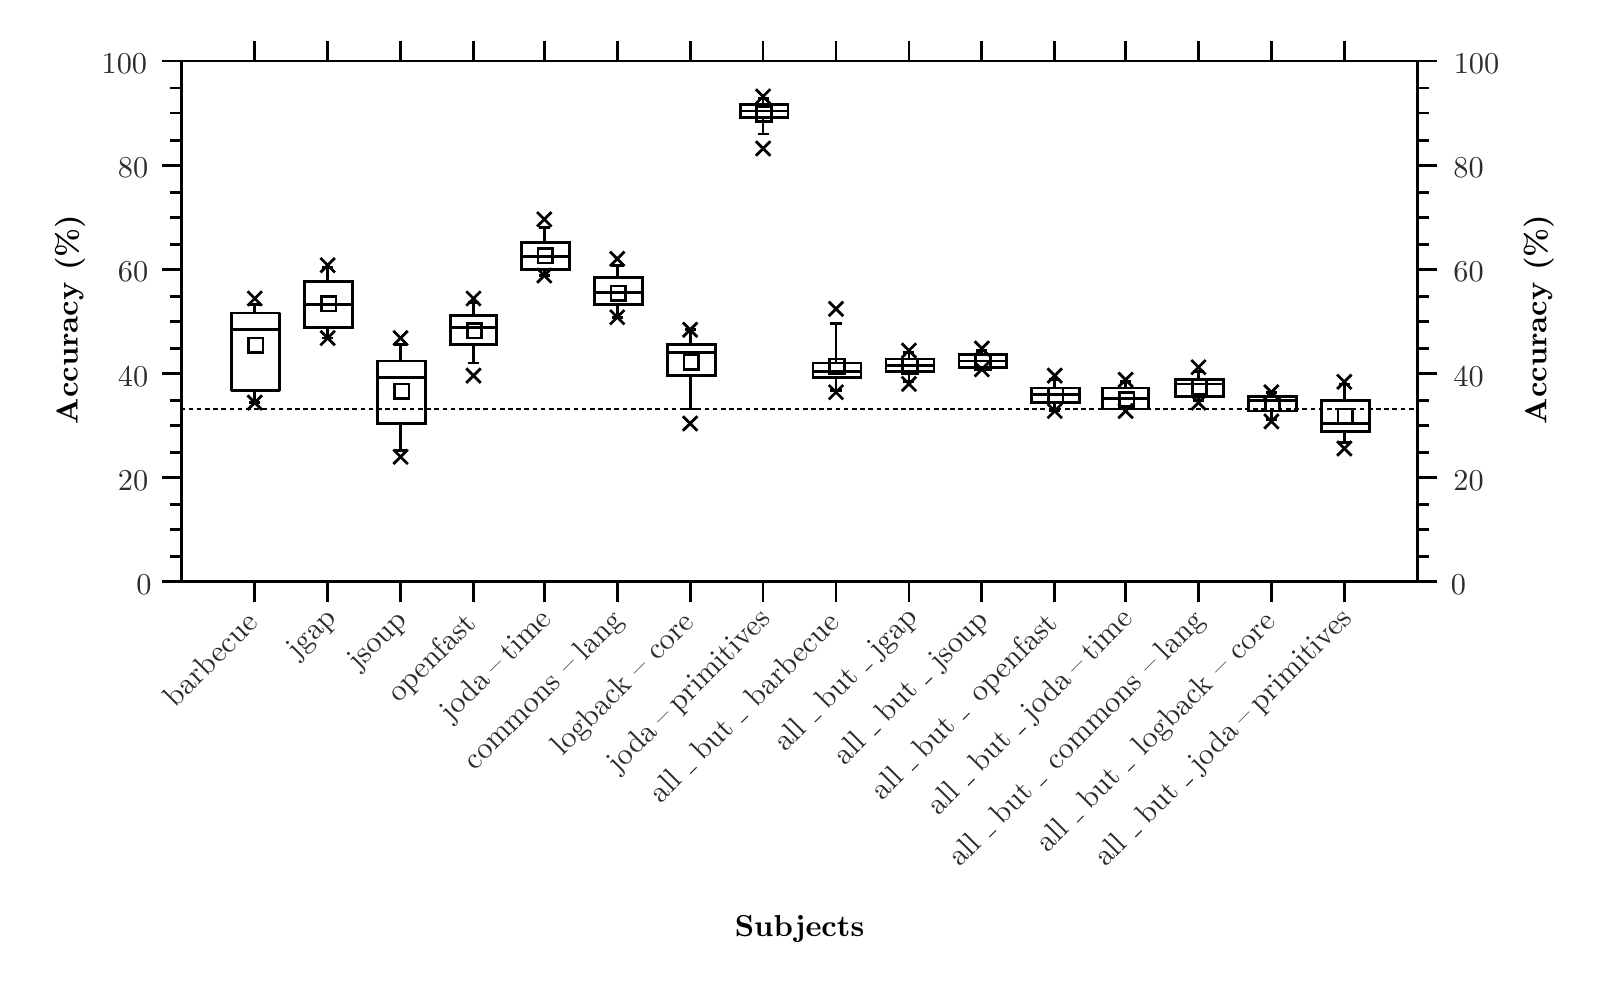
\begin{tikzpicture}{0pt}{0pt}{742pt}{452pt}
	\clip(0pt,452pt) -- (558.587pt,452pt) -- (558.587pt,111.729pt) -- (0pt,111.729pt) -- (0pt,452pt);
\begin{scope}
	\clip(55.7081pt,439.955pt) -- (502.126pt,439.955pt) -- (502.126pt,251.752pt) -- (55.7081pt,251.752pt) -- (55.7081pt,439.955pt);
	\color[rgb]{0,0,0}
	\draw[line width=1pt, line join=bevel, line cap=rect](73.7756pt,348.865pt) -- (91.0903pt,348.865pt) -- (91.0903pt,321.011pt) -- (73.7756pt,321.011pt) -- (73.7756pt,348.865pt);
	\color[rgb]{0,0,0}
	\draw[line width=1pt, line join=bevel, line cap=rect](80.5509pt,316.494pt) -- (83.5622pt,316.494pt);
	\draw[line width=1pt, line join=bevel, line cap=rect](80.5509pt,351.876pt) -- (83.5622pt,351.876pt);
	\draw[line width=1pt, line join=bevel, line cap=rect](82.0566pt,351.876pt) -- (82.0566pt,348.865pt);
	\draw[line width=1pt, line join=bevel, line cap=rect](82.0566pt,316.494pt) -- (82.0566pt,321.011pt);
	\draw[line width=1pt, line join=bevel, line cap=rect](73.7756pt,342.842pt) -- (90.3375pt,342.842pt);
	\draw[line width=1pt, line join=miter, line cap=rect](79.7981pt,318.752pt) -- (84.315pt,314.235pt);
	\draw[line width=1pt, line join=miter, line cap=rect](79.7981pt,314.235pt) -- (84.315pt,318.752pt);
	\draw[line width=1pt, line join=miter, line cap=rect](79.7981pt,356.393pt) -- (84.315pt,351.876pt);
	\draw[line width=1pt, line join=miter, line cap=rect](79.7981pt,351.876pt) -- (84.315pt,356.393pt);
	\draw[line width=1pt, line join=miter, line cap=rect](79.7981pt,339.831pt) -- (85.0678pt,339.831pt) -- (85.0678pt,334.561pt) -- (79.7981pt,334.561pt) -- (79.7981pt,339.831pt);
	\draw[line width=1pt, line join=miter, line cap=rect](100.124pt,360.157pt) -- (117.439pt,360.157pt) -- (117.439pt,343.595pt) -- (100.124pt,343.595pt) -- (100.124pt,360.157pt);
	\draw[line width=1pt, line join=miter, line cap=rect](106.899pt,339.831pt) -- (109.911pt,339.831pt);
	\draw[line width=1pt, line join=miter, line cap=rect](106.899pt,365.427pt) -- (109.911pt,365.427pt);
	\draw[line width=1pt, line join=miter, line cap=rect](108.405pt,365.427pt) -- (108.405pt,360.157pt);
	\draw[line width=1pt, line join=miter, line cap=rect](108.405pt,339.831pt) -- (108.405pt,343.595pt);
	\draw[line width=1pt, line join=miter, line cap=rect](100.124pt,351.876pt) -- (116.686pt,351.876pt);
	\draw[line width=1pt, line join=miter, line cap=rect](106.147pt,342.089pt) -- (110.663pt,337.572pt);
	\draw[line width=1pt, line join=miter, line cap=rect](106.147pt,337.572pt) -- (110.663pt,342.089pt);
	\draw[line width=1pt, line join=miter, line cap=rect](106.147pt,368.438pt) -- (110.663pt,363.921pt);
	\draw[line width=1pt, line join=miter, line cap=rect](106.147pt,363.921pt) -- (110.663pt,368.438pt);
	\draw[line width=1pt, line join=miter, line cap=rect](106.147pt,354.887pt) -- (111.416pt,354.887pt) -- (111.416pt,349.618pt) -- (106.147pt,349.618pt) -- (106.147pt,354.887pt);
	\draw[line width=1pt, line join=miter, line cap=rect](126.472pt,331.55pt) -- (143.787pt,331.55pt) -- (143.787pt,308.966pt) -- (126.472pt,308.966pt) -- (126.472pt,331.55pt);
	\draw[line width=1pt, line join=miter, line cap=rect](133.248pt,299.179pt) -- (136.259pt,299.179pt);
	\draw[line width=1pt, line join=miter, line cap=rect](133.248pt,337.572pt) -- (136.259pt,337.572pt);
	\draw[line width=1pt, line join=miter, line cap=rect](134.753pt,337.572pt) -- (134.753pt,331.55pt);
	\draw[line width=1pt, line join=miter, line cap=rect](134.753pt,299.179pt) -- (134.753pt,308.966pt);
	\draw[line width=1pt, line join=miter, line cap=rect](126.472pt,325.528pt) -- (143.034pt,325.528pt);
	\draw[line width=1pt, line join=miter, line cap=rect](132.495pt,299.179pt) -- (137.012pt,294.662pt);
	\draw[line width=1pt, line join=miter, line cap=rect](132.495pt,294.662pt) -- (137.012pt,299.179pt);
	\draw[line width=1pt, line join=miter, line cap=rect](132.495pt,342.089pt) -- (137.012pt,337.572pt);
	\draw[line width=1pt, line join=miter, line cap=rect](132.495pt,337.572pt) -- (137.012pt,342.089pt);
	\draw[line width=1pt, line join=miter, line cap=rect](132.495pt,323.269pt) -- (137.765pt,323.269pt) -- (137.765pt,317.999pt) -- (132.495pt,317.999pt) -- (132.495pt,323.269pt);
	\draw[line width=1pt, line join=miter, line cap=rect](152.821pt,348.112pt) -- (169.383pt,348.112pt) -- (169.383pt,337.572pt) -- (152.821pt,337.572pt) -- (152.821pt,348.112pt);
	\draw[line width=1pt, line join=miter, line cap=rect](159.596pt,330.797pt) -- (162.607pt,330.797pt);
	\draw[line width=1pt, line join=miter, line cap=rect](159.596pt,352.629pt) -- (162.607pt,352.629pt);
	\draw[line width=1pt, line join=miter, line cap=rect](161.102pt,352.629pt) -- (161.102pt,348.112pt);
	\draw[line width=1pt, line join=miter, line cap=rect](161.102pt,330.797pt) -- (161.102pt,337.572pt);
	\draw[line width=1pt, line join=miter, line cap=rect](152.821pt,343.595pt) -- (169.383pt,343.595pt);
	\draw[line width=1pt, line join=miter, line cap=rect](158.843pt,328.539pt) -- (163.36pt,324.022pt);
	\draw[line width=1pt, line join=miter, line cap=rect](158.843pt,324.022pt) -- (163.36pt,328.539pt);
	\draw[line width=1pt, line join=miter, line cap=rect](158.843pt,356.393pt) -- (163.36pt,351.876pt);
	\draw[line width=1pt, line join=miter, line cap=rect](158.843pt,351.876pt) -- (163.36pt,356.393pt);
	\draw[line width=1pt, line join=miter, line cap=rect](158.843pt,345.101pt) -- (164.113pt,345.101pt) -- (164.113pt,339.831pt) -- (158.843pt,339.831pt) -- (158.843pt,345.101pt);
	\draw[line width=1pt, line join=miter, line cap=rect](178.417pt,374.46pt) -- (195.731pt,374.46pt) -- (195.731pt,364.674pt) -- (178.417pt,364.674pt) -- (178.417pt,374.46pt);
	\draw[line width=1pt, line join=miter, line cap=rect](185.192pt,362.415pt) -- (188.203pt,362.415pt);
	\draw[line width=1pt, line join=miter, line cap=rect](185.192pt,379.73pt) -- (188.203pt,379.73pt);
	\draw[line width=1pt, line join=miter, line cap=rect](186.697pt,379.73pt) -- (186.697pt,374.46pt);
	\draw[line width=1pt, line join=miter, line cap=rect](186.697pt,362.415pt) -- (186.697pt,364.674pt);
	\draw[line width=1pt, line join=miter, line cap=rect](178.417pt,369.191pt) -- (194.978pt,369.191pt);
	\draw[line width=1pt, line join=miter, line cap=rect](184.439pt,364.674pt) -- (188.956pt,360.157pt);
	\draw[line width=1pt, line join=miter, line cap=rect](184.439pt,360.157pt) -- (188.956pt,364.674pt);
	\draw[line width=1pt, line join=miter, line cap=rect](184.439pt,385pt) -- (188.956pt,380.483pt);
	\draw[line width=1pt, line join=miter, line cap=rect](184.439pt,380.483pt) -- (188.956pt,385pt);
	\draw[line width=1pt, line join=miter, line cap=rect](184.439pt,372.202pt) -- (189.709pt,372.202pt) -- (189.709pt,366.932pt) -- (184.439pt,366.932pt) -- (184.439pt,372.202pt);
	\draw[line width=1pt, line join=miter, line cap=rect](204.765pt,361.663pt) -- (222.08pt,361.663pt) -- (222.08pt,351.876pt) -- (204.765pt,351.876pt) -- (204.765pt,361.663pt);
	\draw[line width=1pt, line join=miter, line cap=rect](211.54pt,347.359pt) -- (214.552pt,347.359pt);
	\draw[line width=1pt, line join=miter, line cap=rect](211.54pt,366.179pt) -- (214.552pt,366.179pt);
	\draw[line width=1pt, line join=miter, line cap=rect](213.046pt,366.179pt) -- (213.046pt,361.663pt);
	\draw[line width=1pt, line join=miter, line cap=rect](213.046pt,347.359pt) -- (213.046pt,351.876pt);
	\draw[line width=1pt, line join=miter, line cap=rect](204.765pt,356.393pt) -- (221.327pt,356.393pt);
	\draw[line width=1pt, line join=miter, line cap=rect](210.787pt,349.618pt) -- (215.304pt,345.101pt);
	\draw[line width=1pt, line join=miter, line cap=rect](210.787pt,345.101pt) -- (215.304pt,349.618pt);
	\draw[line width=1pt, line join=miter, line cap=rect](210.787pt,370.696pt) -- (215.304pt,366.179pt);
	\draw[line width=1pt, line join=miter, line cap=rect](210.787pt,366.179pt) -- (215.304pt,370.696pt);
	\draw[line width=1pt, line join=miter, line cap=rect](210.787pt,358.651pt) -- (216.057pt,358.651pt) -- (216.057pt,353.382pt) -- (210.787pt,353.382pt) -- (210.787pt,358.651pt);
	\draw[line width=1pt, line join=miter, line cap=rect](231.113pt,337.572pt) -- (248.428pt,337.572pt) -- (248.428pt,326.28pt) -- (231.113pt,326.28pt) -- (231.113pt,337.572pt);
	\draw[line width=1pt, line join=miter, line cap=rect](237.889pt,314.235pt) -- (240.9pt,314.235pt);
	\draw[line width=1pt, line join=miter, line cap=rect](237.889pt,342.842pt) -- (240.9pt,342.842pt);
	\draw[line width=1pt, line join=miter, line cap=rect](239.394pt,342.842pt) -- (239.394pt,337.572pt);
	\draw[line width=1pt, line join=miter, line cap=rect](239.394pt,314.235pt) -- (239.394pt,326.28pt);
	\draw[line width=1pt, line join=miter, line cap=rect](231.113pt,334.561pt) -- (247.675pt,334.561pt);
	\draw[line width=1pt, line join=miter, line cap=rect](237.136pt,311.224pt) -- (241.653pt,306.707pt);
	\draw[line width=1pt, line join=miter, line cap=rect](237.136pt,306.707pt) -- (241.653pt,311.224pt);
	\draw[line width=1pt, line join=miter, line cap=rect](237.136pt,345.101pt) -- (241.653pt,340.584pt);
	\draw[line width=1pt, line join=miter, line cap=rect](237.136pt,340.584pt) -- (241.653pt,345.101pt);
	\draw[line width=1pt, line join=miter, line cap=rect](237.136pt,333.808pt) -- (242.406pt,333.808pt) -- (242.406pt,328.539pt) -- (237.136pt,328.539pt) -- (237.136pt,333.808pt);
	\draw[line width=1pt, line join=miter, line cap=rect](257.462pt,424.146pt) -- (274.777pt,424.146pt) -- (274.777pt,419.629pt) -- (257.462pt,419.629pt) -- (257.462pt,424.146pt);
	\draw[line width=1pt, line join=miter, line cap=rect](264.237pt,413.607pt) -- (267.248pt,413.607pt);
	\draw[line width=1pt, line join=miter, line cap=rect](264.237pt,426.404pt) -- (267.248pt,426.404pt);
	\draw[line width=1pt, line join=miter, line cap=rect](265.743pt,426.404pt) -- (265.743pt,424.146pt);
	\draw[line width=1pt, line join=miter, line cap=rect](265.743pt,413.607pt) -- (265.743pt,419.629pt);
	\draw[line width=1pt, line join=miter, line cap=rect](257.462pt,421.887pt) -- (274.024pt,421.887pt);
	\draw[line width=1pt, line join=miter, line cap=rect](263.484pt,410.595pt) -- (268.001pt,406.078pt);
	\draw[line width=1pt, line join=miter, line cap=rect](263.484pt,406.078pt) -- (268.001pt,410.595pt);
	\draw[line width=1pt, line join=miter, line cap=rect](263.484pt,429.416pt) -- (268.001pt,424.899pt);
	\draw[line width=1pt, line join=miter, line cap=rect](263.484pt,424.899pt) -- (268.001pt,429.416pt);
	\draw[line width=1pt, line join=miter, line cap=rect](263.484pt,423.393pt) -- (268.754pt,423.393pt) -- (268.754pt,418.123pt) -- (263.484pt,418.123pt) -- (263.484pt,423.393pt);
	\draw[line width=1pt, line join=miter, line cap=rect](283.81pt,330.797pt) -- (301.125pt,330.797pt) -- (301.125pt,325.528pt) -- (283.81pt,325.528pt) -- (283.81pt,330.797pt);
	\draw[line width=1pt, line join=miter, line cap=rect](290.586pt,321.011pt) -- (293.597pt,321.011pt);
	\draw[line width=1pt, line join=miter, line cap=rect](290.586pt,345.101pt) -- (293.597pt,345.101pt);
	\draw[line width=1pt, line join=miter, line cap=rect](292.091pt,345.101pt) -- (292.091pt,330.797pt);
	\draw[line width=1pt, line join=miter, line cap=rect](292.091pt,321.011pt) -- (292.091pt,325.528pt);
	\draw[line width=1pt, line join=miter, line cap=rect](283.81pt,327.786pt) -- (300.372pt,327.786pt);
	\draw[line width=1pt, line join=miter, line cap=rect](289.833pt,322.516pt) -- (294.35pt,317.999pt);
	\draw[line width=1pt, line join=miter, line cap=rect](289.833pt,317.999pt) -- (294.35pt,322.516pt);
	\draw[line width=1pt, line join=miter, line cap=rect](289.833pt,352.629pt) -- (294.35pt,348.112pt);
	\draw[line width=1pt, line join=miter, line cap=rect](289.833pt,348.112pt) -- (294.35pt,352.629pt);
	\draw[line width=1pt, line join=miter, line cap=rect](289.833pt,332.303pt) -- (295.103pt,332.303pt) -- (295.103pt,327.033pt) -- (289.833pt,327.033pt) -- (289.833pt,332.303pt);
	\draw[line width=1pt, line join=miter, line cap=rect](310.159pt,332.303pt) -- (327.473pt,332.303pt) -- (327.473pt,327.786pt) -- (310.159pt,327.786pt) -- (310.159pt,332.303pt);
	\draw[line width=1pt, line join=miter, line cap=rect](316.934pt,324.022pt) -- (319.945pt,324.022pt);
	\draw[line width=1pt, line join=miter, line cap=rect](316.934pt,334.561pt) -- (319.945pt,334.561pt);
	\draw[line width=1pt, line join=miter, line cap=rect](318.44pt,334.561pt) -- (318.44pt,332.303pt);
	\draw[line width=1pt, line join=miter, line cap=rect](318.44pt,324.022pt) -- (318.44pt,327.786pt);
	\draw[line width=1pt, line join=miter, line cap=rect](310.159pt,330.044pt) -- (326.721pt,330.044pt);
	\draw[line width=1pt, line join=miter, line cap=rect](316.181pt,325.528pt) -- (320.698pt,321.011pt);
	\draw[line width=1pt, line join=miter, line cap=rect](316.181pt,321.011pt) -- (320.698pt,325.528pt);
	\draw[line width=1pt, line join=miter, line cap=rect](316.181pt,337.572pt) -- (320.698pt,333.056pt);
	\draw[line width=1pt, line join=miter, line cap=rect](316.181pt,333.056pt) -- (320.698pt,337.572pt);
	\draw[line width=1pt, line join=miter, line cap=rect](316.181pt,332.303pt) -- (321.451pt,332.303pt) -- (321.451pt,327.033pt) -- (316.181pt,327.033pt) -- (316.181pt,332.303pt);
	\draw[line width=1pt, line join=miter, line cap=rect](336.507pt,333.808pt) -- (353.822pt,333.808pt) -- (353.822pt,329.292pt) -- (336.507pt,329.292pt) -- (336.507pt,333.808pt);
	\draw[line width=1pt, line join=miter, line cap=rect](343.282pt,328.539pt) -- (346.294pt,328.539pt);
	\draw[line width=1pt, line join=miter, line cap=rect](343.282pt,335.314pt) -- (346.294pt,335.314pt);
	\draw[line width=1pt, line join=miter, line cap=rect](344.788pt,335.314pt) -- (344.788pt,333.808pt);
	\draw[line width=1pt, line join=miter, line cap=rect](344.788pt,328.539pt) -- (344.788pt,329.292pt);
	\draw[line width=1pt, line join=miter, line cap=rect](336.507pt,331.55pt) -- (353.069pt,331.55pt);
	\draw[line width=1pt, line join=miter, line cap=rect](342.53pt,330.797pt) -- (347.047pt,326.28pt);
	\draw[line width=1pt, line join=miter, line cap=rect](342.53pt,326.28pt) -- (347.047pt,330.797pt);
	\draw[line width=1pt, line join=miter, line cap=rect](342.53pt,338.325pt) -- (347.047pt,333.808pt);
	\draw[line width=1pt, line join=miter, line cap=rect](342.53pt,333.808pt) -- (347.047pt,338.325pt);
	\draw[line width=1pt, line join=miter, line cap=rect](342.53pt,333.808pt) -- (347.799pt,333.808pt) -- (347.799pt,328.539pt) -- (342.53pt,328.539pt) -- (342.53pt,333.808pt);
	\draw[line width=1pt, line join=miter, line cap=rect](362.856pt,321.763pt) -- (380.17pt,321.763pt) -- (380.17pt,316.494pt) -- (362.856pt,316.494pt) -- (362.856pt,321.763pt);
	\draw[line width=1pt, line join=miter, line cap=rect](369.631pt,313.482pt) -- (372.642pt,313.482pt);
	\draw[line width=1pt, line join=miter, line cap=rect](369.631pt,324.775pt) -- (372.642pt,324.775pt);
	\draw[line width=1pt, line join=miter, line cap=rect](371.137pt,324.775pt) -- (371.137pt,321.763pt);
	\draw[line width=1pt, line join=miter, line cap=rect](371.137pt,313.482pt) -- (371.137pt,316.494pt);
	\draw[line width=1pt, line join=miter, line cap=rect](362.856pt,319.505pt) -- (379.418pt,319.505pt);
	\draw[line width=1pt, line join=miter, line cap=rect](368.878pt,315.741pt) -- (373.395pt,311.224pt);
	\draw[line width=1pt, line join=miter, line cap=rect](368.878pt,311.224pt) -- (373.395pt,315.741pt);
	\draw[line width=1pt, line join=miter, line cap=rect](368.878pt,328.539pt) -- (373.395pt,324.022pt);
	\draw[line width=1pt, line join=miter, line cap=rect](368.878pt,324.022pt) -- (373.395pt,328.539pt);
	\draw[line width=1pt, line join=miter, line cap=rect](368.878pt,321.763pt) -- (374.148pt,321.763pt) -- (374.148pt,316.494pt) -- (368.878pt,316.494pt) -- (368.878pt,321.763pt);
	\draw[line width=1pt, line join=miter, line cap=rect](388.451pt,321.763pt) -- (405.013pt,321.763pt) -- (405.013pt,314.235pt) -- (388.451pt,314.235pt) -- (388.451pt,321.763pt);
	\draw[line width=1pt, line join=miter, line cap=rect](395.227pt,314.235pt) -- (398.238pt,314.235pt);
	\draw[line width=1pt, line join=miter, line cap=rect](395.227pt,324.022pt) -- (398.238pt,324.022pt);
	\draw[line width=1pt, line join=miter, line cap=rect](396.732pt,324.022pt) -- (396.732pt,321.763pt);

	\draw[line width=1pt, line join=miter, line cap=rect](388.451pt,317.999pt) -- (405.013pt,317.999pt);
	\draw[line width=1pt, line join=miter, line cap=rect](394.474pt,315.741pt) -- (398.991pt,311.224pt);
	\draw[line width=1pt, line join=miter, line cap=rect](394.474pt,311.224pt) -- (398.991pt,315.741pt);
	\draw[line width=1pt, line join=miter, line cap=rect](394.474pt,327.033pt) -- (398.991pt,322.516pt);
	\draw[line width=1pt, line join=miter, line cap=rect](394.474pt,322.516pt) -- (398.991pt,327.033pt);
	\draw[line width=1pt, line join=miter, line cap=rect](394.474pt,320.258pt) -- (399.743pt,320.258pt) -- (399.743pt,314.988pt) -- (394.474pt,314.988pt) -- (394.474pt,320.258pt);
	\draw[line width=1pt, line join=miter, line cap=rect](414.8pt,324.775pt) -- (432.114pt,324.775pt) -- (432.114pt,318.752pt) -- (414.8pt,318.752pt) -- (414.8pt,324.775pt);
	\draw[line width=1pt, line join=miter, line cap=rect](421.575pt,317.247pt) -- (424.586pt,317.247pt);
	\draw[line width=1pt, line join=miter, line cap=rect](421.575pt,327.786pt) -- (424.586pt,327.786pt);
	\draw[line width=1pt, line join=miter, line cap=rect](423.081pt,327.786pt) -- (423.081pt,324.775pt);
	\draw[line width=1pt, line join=miter, line cap=rect](423.081pt,317.247pt) -- (423.081pt,318.752pt);
	\draw[line width=1pt, line join=miter, line cap=rect](414.8pt,323.269pt) -- (431.362pt,323.269pt);
	\draw[line width=1pt, line join=miter, line cap=rect](420.822pt,318.752pt) -- (425.339pt,314.235pt);
	\draw[line width=1pt, line join=miter, line cap=rect](420.822pt,314.235pt) -- (425.339pt,318.752pt);
	\draw[line width=1pt, line join=miter, line cap=rect](420.822pt,331.55pt) -- (425.339pt,327.033pt);
	\draw[line width=1pt, line join=miter, line cap=rect](420.822pt,327.033pt) -- (425.339pt,331.55pt);
	\draw[line width=1pt, line join=miter, line cap=rect](420.822pt,324.775pt) -- (426.092pt,324.775pt) -- (426.092pt,319.505pt) -- (420.822pt,319.505pt) -- (420.822pt,324.775pt);
	\draw[line width=1pt, line join=miter, line cap=rect](441.148pt,318.752pt) -- (458.463pt,318.752pt) -- (458.463pt,313.482pt) -- (441.148pt,313.482pt) -- (441.148pt,318.752pt);
	\draw[line width=1pt, line join=miter, line cap=rect](447.923pt,310.471pt) -- (450.935pt,310.471pt);
	\draw[line width=1pt, line join=miter, line cap=rect](447.923pt,320.258pt) -- (450.935pt,320.258pt);
	\draw[line width=1pt, line join=miter, line cap=rect](449.429pt,320.258pt) -- (449.429pt,318.752pt);
	\draw[line width=1pt, line join=miter, line cap=rect](449.429pt,310.471pt) -- (449.429pt,313.482pt);
	\draw[line width=1pt, line join=miter, line cap=rect](441.148pt,317.247pt) -- (457.71pt,317.247pt);
	\draw[line width=1pt, line join=miter, line cap=rect](447.171pt,311.977pt) -- (451.688pt,307.46pt);
	\draw[line width=1pt, line join=miter, line cap=rect](447.171pt,307.46pt) -- (451.688pt,311.977pt);
	\draw[line width=1pt, line join=miter, line cap=rect](447.171pt,322.516pt) -- (451.688pt,317.999pt);
	\draw[line width=1pt, line join=miter, line cap=rect](447.171pt,317.999pt) -- (451.688pt,322.516pt);
	\draw[line width=1pt, line join=miter, line cap=rect](447.171pt,318.752pt) -- (452.44pt,318.752pt) -- (452.44pt,313.482pt) -- (447.171pt,313.482pt) -- (447.171pt,318.752pt);
	\draw[line width=1pt, line join=miter, line cap=rect](467.497pt,317.247pt) -- (484.811pt,317.247pt) -- (484.811pt,305.954pt) -- (467.497pt,305.954pt) -- (467.497pt,317.247pt);
	\draw[line width=1pt, line join=miter, line cap=rect](474.272pt,302.19pt) -- (477.283pt,302.19pt);
	\draw[line width=1pt, line join=miter, line cap=rect](474.272pt,323.269pt) -- (477.283pt,323.269pt);
	\draw[line width=1pt, line join=miter, line cap=rect](475.777pt,323.269pt) -- (475.777pt,317.247pt);
	\draw[line width=1pt, line join=miter, line cap=rect](475.777pt,302.19pt) -- (475.777pt,305.954pt);
	\draw[line width=1pt, line join=miter, line cap=rect](467.497pt,308.966pt) -- (484.058pt,308.966pt);
	\draw[line width=1pt, line join=miter, line cap=rect](473.519pt,302.19pt) -- (478.036pt,297.673pt);
	\draw[line width=1pt, line join=miter, line cap=rect](473.519pt,297.673pt) -- (478.036pt,302.19pt);
	\draw[line width=1pt, line join=miter, line cap=rect](473.519pt,326.28pt) -- (478.036pt,321.763pt);
	\draw[line width=1pt, line join=miter, line cap=rect](473.519pt,321.763pt) -- (478.036pt,326.28pt);
	\draw[line width=1pt, line join=miter, line cap=rect](473.519pt,314.235pt) -- (478.789pt,314.235pt) -- (478.789pt,308.966pt) -- (473.519pt,308.966pt) -- (473.519pt,314.235pt);


	\draw[line width=1pt, dash pattern=on 0.024cm off 0.08cm, dash phase=0pt, line join=miter, line cap=rect](55.7081pt,314.235pt) -- (528.474pt,314.235pt);
\end{scope}
\begin{scope}
	\color[rgb]{0,0,0}
	\pgftext[center, base, at={\pgfpoint{18.0675pt}{346.606pt}},rotate=90]{\fontsize{11}{0}\selectfont{\textbf{Accuracy (\%)}}}
	\color[rgb]{0.172549,0.172549,0.172549}
	\pgftext[center, base, at={\pgfpoint{42.0163pt}{247.235pt}}]{\fontsize{11}{0}\selectfont{0}}
	\pgftext[center, base, at={\pgfpoint{38.1111pt}{284.876pt}}]{\fontsize{11}{0}\selectfont{20}}
	\pgftext[center, base, at={\pgfpoint{38.1111pt}{322.516pt}}]{\fontsize{11}{0}\selectfont{40}}
	\pgftext[center, base, at={\pgfpoint{38.1111pt}{360.157pt}}]{\fontsize{11}{0}\selectfont{60}}
	\pgftext[center, base, at={\pgfpoint{38.1111pt}{397.798pt}}]{\fontsize{11}{0}\selectfont{80}}
	\pgftext[center, base, at={\pgfpoint{34.9587pt}{435.438pt}}]{\fontsize{11}{0}\selectfont{100}}
	\color[rgb]{0,0,0}
	\draw[line width=1pt, line join=bevel, line cap=rect](55.7081pt,260.786pt) -- (51.9441pt,260.786pt);
	\draw[line width=1pt, line join=bevel, line cap=rect](55.7081pt,279.606pt) -- (51.9441pt,279.606pt);
	\draw[line width=1pt, line join=bevel, line cap=rect](55.7081pt,298.426pt) -- (51.9441pt,298.426pt);
	\draw[line width=1pt, line join=bevel, line cap=rect](55.7081pt,317.247pt) -- (51.9441pt,317.247pt);
	\draw[line width=1pt, line join=bevel, line cap=rect](55.7081pt,336.067pt) -- (51.9441pt,336.067pt);
	\draw[line width=1pt, line join=bevel, line cap=rect](55.7081pt,354.887pt) -- (51.9441pt,354.887pt);
	\draw[line width=1pt, line join=bevel, line cap=rect](55.7081pt,373.707pt) -- (51.9441pt,373.707pt);
	\draw[line width=1pt, line join=bevel, line cap=rect](55.7081pt,392.528pt) -- (51.9441pt,392.528pt);
	\draw[line width=1pt, line join=bevel, line cap=rect](55.7081pt,411.348pt) -- (51.9441pt,411.348pt);
	\draw[line width=1pt, line join=bevel, line cap=rect](55.7081pt,430.168pt) -- (51.9441pt,430.168pt);
	\draw[line width=1pt, line join=bevel, line cap=rect](55.7081pt,270.572pt) -- (51.9441pt,270.572pt);
	\draw[line width=1pt, line join=bevel, line cap=rect](55.7081pt,308.213pt) -- (51.9441pt,308.213pt);
	\draw[line width=1pt, line join=bevel, line cap=rect](55.7081pt,345.853pt) -- (51.9441pt,345.853pt);
	\draw[line width=1pt, line join=bevel, line cap=rect](55.7081pt,383.494pt) -- (51.9441pt,383.494pt);
	\draw[line width=1pt, line join=bevel, line cap=rect](55.7081pt,421.135pt) -- (51.9441pt,421.135pt);
	\draw[line width=1pt, line join=bevel, line cap=rect](55.7081pt,251.752pt) -- (48.9328pt,251.752pt);
	\draw[line width=1pt, line join=bevel, line cap=rect](55.7081pt,289.393pt) -- (48.9328pt,289.393pt);
	\draw[line width=1pt, line join=bevel, line cap=rect](55.7081pt,327.033pt) -- (48.9328pt,327.033pt);
	\draw[line width=1pt, line join=bevel, line cap=rect](55.7081pt,364.674pt) -- (48.9328pt,364.674pt);
	\draw[line width=1pt, line join=bevel, line cap=rect](55.7081pt,402.314pt) -- (48.9328pt,402.314pt);
	\draw[line width=1pt, line join=bevel, line cap=rect](55.7081pt,439.955pt) -- (48.9328pt,439.955pt);
	\draw[line width=1pt, line join=bevel, line cap=rect](55.7081pt,439.955pt) -- (55.7081pt,251.752pt);
	\pgftext[center, base, at={\pgfpoint{548.8pt}{346.606pt}},rotate=90]{\fontsize{11}{0}\selectfont{\textbf{Accuracy (\%)}}}
	\color[rgb]{0.172549,0.172549,0.172549}
	\pgftext[center, base, at={\pgfpoint{517.041pt}{247.235pt}}]{\fontsize{11}{0}\selectfont{0}}
	\pgftext[center, base, at={\pgfpoint{520.664pt}{284.876pt}}]{\fontsize{11}{0}\selectfont{20}}
	\pgftext[center, base, at={\pgfpoint{520.664pt}{322.516pt}}]{\fontsize{11}{0}\selectfont{40}}
	\pgftext[center, base, at={\pgfpoint{520.664pt}{360.157pt}}]{\fontsize{11}{0}\selectfont{60}}
	\pgftext[center, base, at={\pgfpoint{520.664pt}{397.798pt}}]{\fontsize{11}{0}\selectfont{80}}
	\pgftext[center, base, at={\pgfpoint{523.534pt}{435.438pt}}]{\fontsize{11}{0}\selectfont{100}}
	\color[rgb]{0,0,0}
	\draw[line width=1pt, line join=bevel, line cap=rect](502.126pt,260.786pt) -- (505.89pt,260.786pt);
	\draw[line width=1pt, line join=bevel, line cap=rect](502.126pt,279.606pt) -- (505.89pt,279.606pt);
	\draw[line width=1pt, line join=bevel, line cap=rect](502.126pt,298.426pt) -- (505.89pt,298.426pt);
	\draw[line width=1pt, line join=bevel, line cap=rect](502.126pt,317.247pt) -- (505.89pt,317.247pt);
	\draw[line width=1pt, line join=bevel, line cap=rect](502.126pt,336.067pt) -- (505.89pt,336.067pt);
	\draw[line width=1pt, line join=bevel, line cap=rect](502.126pt,354.887pt) -- (505.89pt,354.887pt);
	\draw[line width=1pt, line join=bevel, line cap=rect](502.126pt,373.707pt) -- (505.89pt,373.707pt);
	\draw[line width=1pt, line join=bevel, line cap=rect](502.126pt,392.528pt) -- (505.89pt,392.528pt);
	\draw[line width=1pt, line join=bevel, line cap=rect](502.126pt,411.348pt) -- (505.89pt,411.348pt);
	\draw[line width=1pt, line join=bevel, line cap=rect](502.126pt,430.168pt) -- (505.89pt,430.168pt);
	\draw[line width=1pt, line join=bevel, line cap=rect](502.126pt,270.572pt) -- (505.89pt,270.572pt);
	\draw[line width=1pt, line join=bevel, line cap=rect](502.126pt,308.213pt) -- (505.89pt,308.213pt);
	\draw[line width=1pt, line join=bevel, line cap=rect](502.126pt,345.853pt) -- (505.89pt,345.853pt);
	\draw[line width=1pt, line join=bevel, line cap=rect](502.126pt,383.494pt) -- (505.89pt,383.494pt);
	\draw[line width=1pt, line join=bevel, line cap=rect](502.126pt,421.135pt) -- (505.89pt,421.135pt);
	\draw[line width=1pt, line join=bevel, line cap=rect](502.126pt,251.752pt) -- (508.901pt,251.752pt);
	\draw[line width=1pt, line join=bevel, line cap=rect](502.126pt,289.393pt) -- (508.901pt,289.393pt);
	\draw[line width=1pt, line join=bevel, line cap=rect](502.126pt,327.033pt) -- (508.901pt,327.033pt);
	\draw[line width=1pt, line join=bevel, line cap=rect](502.126pt,364.674pt) -- (508.901pt,364.674pt);
	\draw[line width=1pt, line join=bevel, line cap=rect](502.126pt,402.314pt) -- (508.901pt,402.314pt);
	\draw[line width=1pt, line join=bevel, line cap=rect](502.126pt,439.955pt) -- (508.901pt,439.955pt);
	\draw[line width=1pt, line join=bevel, line cap=rect](502.126pt,439.955pt) -- (502.126pt,251.752pt);
	\pgftext[center, base, at={\pgfpoint{278.917pt}{123.774pt}}]{\fontsize{11}{0}\selectfont{\textbf{Subjects}}}
	\color[rgb]{0.172549,0.172549,0.172549}
	\pgftext[center, base, at={\pgfpoint{68.4991pt}{221.267pt}},rotate=45]{\fontsize{11}{0}\selectfont{barbecue}}
	\pgftext[center, base, at={\pgfpoint{104.654pt}{231.073pt}},rotate=45]{\fontsize{11}{0}\selectfont{jgap}}
	\pgftext[center, base, at={\pgfpoint{128.445pt}{228.516pt}},rotate=45]{\fontsize{11}{0}\selectfont{jsoup}}
	\pgftext[center, base, at={\pgfpoint{148.222pt}{221.945pt}},rotate=45]{\fontsize{11}{0}\selectfont{openfast}}
	\pgftext[center, base, at={\pgfpoint{160.198pt}{208.325pt}},rotate=45]{\fontsize{11}{0}\selectfont{joda}}
	\pgftext[center, base, at={\pgfpoint{171.111pt}{219.238pt}},rotate=45]{\fontsize{11}{0}\selectfont{--}}
	\pgftext[center, base, at={\pgfpoint{182.11pt}{230.238pt}},rotate=45]{\fontsize{11}{0}\selectfont{time}}
	\pgftext[center, base, at={\pgfpoint{177.272pt}{199.051pt}},rotate=45]{\fontsize{11}{0}\selectfont{commons}}
	\pgftext[center, base, at={\pgfpoint{197.542pt}{219.321pt}},rotate=45]{\fontsize{11}{0}\selectfont{--}}
	\pgftext[center, base, at={\pgfpoint{208.405pt}{230.184pt}},rotate=45]{\fontsize{11}{0}\selectfont{lang}}
	\pgftext[center, base, at={\pgfpoint{205.896pt}{201.326pt}},rotate=45]{\fontsize{11}{0}\selectfont{logback}}
	\pgftext[center, base, at={\pgfpoint{223.117pt}{218.547pt}},rotate=45]{\fontsize{11}{0}\selectfont{--}}
	\pgftext[center, base, at={\pgfpoint{234.342pt}{229.772pt}},rotate=45]{\fontsize{11}{0}\selectfont{core}}
	\pgftext[center, base, at={\pgfpoint{220.612pt}{189.694pt}},rotate=45]{\fontsize{11}{0}\selectfont{joda}}
	\pgftext[center, base, at={\pgfpoint{231.525pt}{200.607pt}},rotate=45]{\fontsize{11}{0}\selectfont{--}}
	\pgftext[center, base, at={\pgfpoint{252.027pt}{221.109pt}},rotate=45]{\fontsize{11}{0}\selectfont{primitives}}
	\pgftext[center, base, at={\pgfpoint{232.684pt}{175.417pt}},rotate=45]{\fontsize{11}{0}\selectfont{all}}
	\pgftext[center, base, at={\pgfpoint{240.498pt}{183.231pt}},rotate=45]{\fontsize{11}{0}\selectfont{\_}}
	\pgftext[center, base, at={\pgfpoint{249.743pt}{192.476pt}},rotate=45]{\fontsize{11}{0}\selectfont{but}}
	\pgftext[center, base, at={\pgfpoint{258.988pt}{201.721pt}},rotate=45]{\fontsize{11}{0}\selectfont{\_}}
	\pgftext[center, base, at={\pgfpoint{278.584pt}{221.317pt}},rotate=45]{\fontsize{11}{0}\selectfont{barbecue}}
	\pgftext[center, base, at={\pgfpoint{277.663pt}{194.048pt}},rotate=45]{\fontsize{11}{0}\selectfont{all}}
	\pgftext[center, base, at={\pgfpoint{285.478pt}{201.862pt}},rotate=45]{\fontsize{11}{0}\selectfont{\_}}
	\pgftext[center, base, at={\pgfpoint{294.722pt}{211.107pt}},rotate=45]{\fontsize{11}{0}\selectfont{but}}
	\pgftext[center, base, at={\pgfpoint{303.967pt}{220.352pt}},rotate=45]{\fontsize{11}{0}\selectfont{\_}}
	\pgftext[center, base, at={\pgfpoint{314.738pt}{231.123pt}},rotate=45]{\fontsize{11}{0}\selectfont{jgap}}
	\pgftext[center, base, at={\pgfpoint{299.221pt}{189.257pt}},rotate=45]{\fontsize{11}{0}\selectfont{all}}
	\pgftext[center, base, at={\pgfpoint{307.035pt}{197.072pt}},rotate=45]{\fontsize{11}{0}\selectfont{\_}}
	\pgftext[center, base, at={\pgfpoint{316.28pt}{206.317pt}},rotate=45]{\fontsize{11}{0}\selectfont{but}}
	\pgftext[center, base, at={\pgfpoint{325.525pt}{215.561pt}},rotate=45]{\fontsize{11}{0}\selectfont{\_}}
	\pgftext[center, base, at={\pgfpoint{338.529pt}{228.566pt}},rotate=45]{\fontsize{11}{0}\selectfont{jsoup}}
	\pgftext[center, base, at={\pgfpoint{312.794pt}{176.482pt}},rotate=45]{\fontsize{11}{0}\selectfont{all}}
	\pgftext[center, base, at={\pgfpoint{320.608pt}{184.296pt}},rotate=45]{\fontsize{11}{0}\selectfont{\_}}
	\pgftext[center, base, at={\pgfpoint{329.853pt}{193.541pt}},rotate=45]{\fontsize{11}{0}\selectfont{but}}
	\pgftext[center, base, at={\pgfpoint{339.098pt}{202.786pt}},rotate=45]{\fontsize{11}{0}\selectfont{\_}}
	\pgftext[center, base, at={\pgfpoint{358.307pt}{221.995pt}},rotate=45]{\fontsize{11}{0}\selectfont{openfast}}
	\pgftext[center, base, at={\pgfpoint{333.066pt}{171.159pt}},rotate=45]{\fontsize{11}{0}\selectfont{all}}
	\pgftext[center, base, at={\pgfpoint{340.88pt}{178.973pt}},rotate=45]{\fontsize{11}{0}\selectfont{\_}}
	\pgftext[center, base, at={\pgfpoint{350.125pt}{188.218pt}},rotate=45]{\fontsize{11}{0}\selectfont{but}}
	\pgftext[center, base, at={\pgfpoint{359.37pt}{197.463pt}},rotate=45]{\fontsize{11}{0}\selectfont{\_}}
	\pgftext[center, base, at={\pgfpoint{370.283pt}{208.375pt}},rotate=45]{\fontsize{11}{0}\selectfont{joda}}
	\pgftext[center, base, at={\pgfpoint{381.195pt}{219.288pt}},rotate=45]{\fontsize{11}{0}\selectfont{--}}
	\pgftext[center, base, at={\pgfpoint{392.195pt}{230.287pt}},rotate=45]{\fontsize{11}{0}\selectfont{time}}
	\pgftext[center, base, at={\pgfpoint{340.783pt}{152.527pt}},rotate=45]{\fontsize{11}{0}\selectfont{all}}
	\pgftext[center, base, at={\pgfpoint{348.598pt}{160.342pt}},rotate=45]{\fontsize{11}{0}\selectfont{\_}}
	\pgftext[center, base, at={\pgfpoint{357.842pt}{169.587pt}},rotate=45]{\fontsize{11}{0}\selectfont{but}}
	\pgftext[center, base, at={\pgfpoint{367.087pt}{178.831pt}},rotate=45]{\fontsize{11}{0}\selectfont{\_}}
	\pgftext[center, base, at={\pgfpoint{387.357pt}{199.101pt}},rotate=45]{\fontsize{11}{0}\selectfont{commons}}
	\pgftext[center, base, at={\pgfpoint{407.627pt}{219.371pt}},rotate=45]{\fontsize{11}{0}\selectfont{--}}
	\pgftext[center, base, at={\pgfpoint{418.489pt}{230.233pt}},rotate=45]{\fontsize{11}{0}\selectfont{lang}}
	\pgftext[center, base, at={\pgfpoint{372.455pt}{157.851pt}},rotate=45]{\fontsize{11}{0}\selectfont{all}}
	\pgftext[center, base, at={\pgfpoint{380.269pt}{165.665pt}},rotate=45]{\fontsize{11}{0}\selectfont{\_}}
	\pgftext[center, base, at={\pgfpoint{389.514pt}{174.91pt}},rotate=45]{\fontsize{11}{0}\selectfont{but}}
	\pgftext[center, base, at={\pgfpoint{398.759pt}{184.155pt}},rotate=45]{\fontsize{11}{0}\selectfont{\_}}
	\pgftext[center, base, at={\pgfpoint{415.98pt}{201.376pt}},rotate=45]{\fontsize{11}{0}\selectfont{logback}}
	\pgftext[center, base, at={\pgfpoint{433.202pt}{218.597pt}},rotate=45]{\fontsize{11}{0}\selectfont{--}}
	\pgftext[center, base, at={\pgfpoint{444.426pt}{229.822pt}},rotate=45]{\fontsize{11}{0}\selectfont{core}}
	\pgftext[center, base, at={\pgfpoint{393.48pt}{152.527pt}},rotate=45]{\fontsize{11}{0}\selectfont{all}}
	\pgftext[center, base, at={\pgfpoint{401.294pt}{160.342pt}},rotate=45]{\fontsize{11}{0}\selectfont{\_}}
	\pgftext[center, base, at={\pgfpoint{410.539pt}{169.587pt}},rotate=45]{\fontsize{11}{0}\selectfont{but}}
	\pgftext[center, base, at={\pgfpoint{419.784pt}{178.831pt}},rotate=45]{\fontsize{11}{0}\selectfont{\_}}
	\pgftext[center, base, at={\pgfpoint{430.697pt}{189.744pt}},rotate=45]{\fontsize{11}{0}\selectfont{joda}}
	\pgftext[center, base, at={\pgfpoint{441.609pt}{200.656pt}},rotate=45]{\fontsize{11}{0}\selectfont{--}}
	\pgftext[center, base, at={\pgfpoint{462.112pt}{221.159pt}},rotate=45]{\fontsize{11}{0}\selectfont{primitives}}
	\color[rgb]{0,0,0}
	\draw[line width=1pt, line join=bevel, line cap=rect](82.0566pt,251.752pt) -- (82.0566pt,244.977pt);
	\draw[line width=1pt, line join=bevel, line cap=rect](108.405pt,251.752pt) -- (108.405pt,244.977pt);
	\draw[line width=1pt, line join=bevel, line cap=rect](134.753pt,251.752pt) -- (134.753pt,244.977pt);
	\draw[line width=1pt, line join=bevel, line cap=rect](161.102pt,251.752pt) -- (161.102pt,244.977pt);
	\draw[line width=1pt, line join=bevel, line cap=rect](186.697pt,251.752pt) -- (186.697pt,244.977pt);
	\draw[line width=1pt, line join=bevel, line cap=rect](213.046pt,251.752pt) -- (213.046pt,244.977pt);
	\draw[line width=1pt, line join=bevel, line cap=rect](239.394pt,251.752pt) -- (239.394pt,244.977pt);
	\draw[line width=1pt, line join=bevel, line cap=rect](265.743pt,251.752pt) -- (265.743pt,244.977pt);
	\draw[line width=1pt, line join=bevel, line cap=rect](292.091pt,251.752pt) -- (292.091pt,244.977pt);
	\draw[line width=1pt, line join=bevel, line cap=rect](318.44pt,251.752pt) -- (318.44pt,244.977pt);
	\draw[line width=1pt, line join=bevel, line cap=rect](344.788pt,251.752pt) -- (344.788pt,244.977pt);
	\draw[line width=1pt, line join=bevel, line cap=rect](371.137pt,251.752pt) -- (371.137pt,244.977pt);
	\draw[line width=1pt, line join=bevel, line cap=rect](396.732pt,251.752pt) -- (396.732pt,244.977pt);
	\draw[line width=1pt, line join=bevel, line cap=rect](423.081pt,251.752pt) -- (423.081pt,244.977pt);
	\draw[line width=1pt, line join=bevel, line cap=rect](449.429pt,251.752pt) -- (449.429pt,244.977pt);
	\draw[line width=1pt, line join=bevel, line cap=rect](475.777pt,251.752pt) -- (475.777pt,244.977pt);
	\draw[line width=1pt, line join=bevel, line cap=rect](55.7081pt,251.752pt) -- (502.126pt,251.752pt);
	\draw[line width=1pt, line join=bevel, line cap=rect](82.0566pt,439.955pt) -- (82.0566pt,446.73pt);
	\draw[line width=1pt, line join=bevel, line cap=rect](108.405pt,439.955pt) -- (108.405pt,446.73pt);
	\draw[line width=1pt, line join=bevel, line cap=rect](134.753pt,439.955pt) -- (134.753pt,446.73pt);
	\draw[line width=1pt, line join=bevel, line cap=rect](161.102pt,439.955pt) -- (161.102pt,446.73pt);
	\draw[line width=1pt, line join=bevel, line cap=rect](186.697pt,439.955pt) -- (186.697pt,446.73pt);
	\draw[line width=1pt, line join=bevel, line cap=rect](213.046pt,439.955pt) -- (213.046pt,446.73pt);
	\draw[line width=1pt, line join=bevel, line cap=rect](239.394pt,439.955pt) -- (239.394pt,446.73pt);
	\draw[line width=1pt, line join=bevel, line cap=rect](265.743pt,439.955pt) -- (265.743pt,446.73pt);
	\draw[line width=1pt, line join=bevel, line cap=rect](292.091pt,439.955pt) -- (292.091pt,446.73pt);
	\draw[line width=1pt, line join=bevel, line cap=rect](318.44pt,439.955pt) -- (318.44pt,446.73pt);
	\draw[line width=1pt, line join=bevel, line cap=rect](344.788pt,439.955pt) -- (344.788pt,446.73pt);
	\draw[line width=1pt, line join=bevel, line cap=rect](371.137pt,439.955pt) -- (371.137pt,446.73pt);
	\draw[line width=1pt, line join=bevel, line cap=rect](396.732pt,439.955pt) -- (396.732pt,446.73pt);
	\draw[line width=1pt, line join=bevel, line cap=rect](423.081pt,439.955pt) -- (423.081pt,446.73pt);
	\draw[line width=1pt, line join=bevel, line cap=rect](449.429pt,439.955pt) -- (449.429pt,446.73pt);
	\draw[line width=1pt, line join=bevel, line cap=rect](475.777pt,439.955pt) -- (475.777pt,446.73pt);
	\draw[line width=1pt, line join=bevel, line cap=rect](55.7081pt,439.955pt) -- (502.126pt,439.955pt);
\end{scope}
\end{tikzpicture}

  \end{adjustbox}
  \caption{Method-level training and prediction accuracy over the eight test subjects and sets of \emph{all\_but\_<subject>}.}
  \vspace{2mm}
  \hrule
  \label{fig:prediction_method_graph}
\end{figure}

We present the results of training and prediction for class- and method-level in Figures~\ref{fig:prediction_class_graph}~and~\ref{fig:prediction_method_graph}. We can see a common trend in both class- and method-level source code units for prediction accuracy, the individual test subjects have a much wider variation in accuracy, while the variation in the \emph{all\_but\_<subject>} is less so. This is mainly due to the low amount of training data provided due to undersampling as we previously mentioned in Section~\ref{subsec:experiment_cross_validation} using Table~\ref{tab:experiments_undersampled_data}. In the class-level accuracies, we can see that a number of the test subjects have variations in their accuracy that was actually 0\%. In these situations nothing was predicted correctly, we describe why this might be occurring in Section~\ref{subsec:experiment_optimization_generalization}. A number of the class-level test subjects mean accuracies are just above or below the random value of 33.3333\%, which is a little disappointing. On the contrary, method-level test subjects mostly perform much better then their class-level counterparts. We see the similar trends from cross-validation (see Section~\ref{subsec:experiment_cross_validation}) for \emph{joda-primitives} and \emph{joda-time} for method-level accuracies. The differences between the class- and method-level source code unit prediction of unknown data is interesting and could be a cause of the two following factors:

\begin{itemize}
  \item Classes have much more factors involved in them (i.e., a set of methods) thus harder to predict.
  \item Our approach does not account for overloaded, anonymous, and abstract methods thus the classes are partially incomplete in data.
\end{itemize}


\subsection{Optimization and Generalization}
\label{subsec:experiment_optimization_generalization}
\begin{quote}
  \emph{\textbf{Research Question \#1:} Can we optimize our approach to achieve better performance by using a different measure of classifier performance?}
\end{quote}

\begin{quote}
  \emph{\textbf{Research Question \#2:} Can we identify a general set of \gls{svm} parameters that maximize mutation score prediction performance on unknown data?}
\end{quote}

\noindent
We keep track of the frequency of parameter pairs selected over all the prediction experiments conducted in Section~\ref{subsec:experiment_prediction}. As a result of LIBSVM's \emph{easy script}, we saw 57 different pairings of the LIBSVM parameters \emph{cost} and \emph{gamma} (described in Section~\ref{subsec:background_support_vector_machine}). This indicates that the classifiers are being tuned specifically to maximize the cross-validation accuracy. Due to undersampling, different parameters are being used to ensure this maximization of cross-validation accuracy. To encourage generalization of unknown projects and data, ideally we want to find a parameter pairing that maximizes generalizability and classification performance on unknown data. As our approach initially requires mutation testing results to perform training it might be appropriate to select the best parameters for the given data. In the previous section for predictions on unknown data (see Section~\ref{subsec:experiment_prediction}), we included the \emph{all\_but\_<subject>} data sets which for our approach do not require us to have the mutation score for practical usage. In this situation it becomes much more clear on why we need a generalizable set of parameters that hopefully performance well on most test subjects. In terms of usability if we can find a general set of parameters for predicting mutation scores, this will lessen the need to specifically tune every classifier prior to prediction.

\begin{sidewaysfigure}[!tb]
  \centering
  \caption{Raw output of training on \texttt{joda-time} then predicting on its unknowns using the parameters \emph{cost}=0.03125 and \emph{gamma}=0.0078125.}
  \label{fig:raw_output_bad}
  \begin{minipage}{.95\textheight}
  \scriptsize{
  \lstinputlisting[language=Java, basicstyle=\fontsize{3.3mm}{4.3mm}\ttfamily,]{listings/raw_output_bad.txt}
  }
  \end{minipage}
  
  \vspace{3em}

  \centering
  \caption{Raw output of training on \texttt{joda-time} then predicting on its unknowns using the parameters \emph{cost}=8 and \emph{gamma}=0.125.}
  \label{fig:raw_output_good}
  \begin{minipage}{.95\textheight}
  \scriptsize{
  \lstinputlisting[language=Java, basicstyle=\fontsize{3.3mm}{4.3mm}\ttfamily,]{listings/raw_output_good.txt}
  }
  \end{minipage}
\end{sidewaysfigure}
\afterpage\clearpage

We noticed that in some situations accuracy is not the best measure for a classifier's effectiveness. For example, consider the following situation: Given imbalanced data for the testing/unknown data set, the accuracy could misrepresent the performance of the classifier. The raw outputs of our classifier using two different sets of parameters on the \emph{joda-time} subject are shown in Figures~\ref{fig:raw_output_bad}~and~\ref{fig:raw_output_good}. In both of the raw outputs we can see a confusion matrix along with performance measures. We can see in the raw output in Figure~\ref{fig:raw_output_bad} that all of predictions fall in category \texttt{2}. The \emph{joda-time} data set is imbalanced with the majority of data (i.e., 76.1675\% of the data) belonging to category \texttt{2}. Even with the biased predictions made towards the majority category, the accuracy of the prediction is 76.1675\%. In contrast to the the raw output presented in Figure~\ref{fig:raw_output_good} we can see that the accuracy is slightly lower at 71.7391\%. Now even though the accuracy in the second example is slightly lower we can consider it a superior classifier to the former as it actually treats the categories in a more unbiased fashion (i.e., one category is not receiving the majority of predictions like the previous example). To alleviate this problem, we consider other measurements that can be used to assess the predictive capabilities of classifiers, specifically the following measures:

\begin{itemize}
  \item \textbf{F-score} represents the harmonic mean of the recall and precision for a category~\cite{SJS06}. A score closer to 1 (i.e., 100\%) represents better performance.
  \begin{equation}
    \emph{$\text{F-score} = 2*\frac{recall * precision}{recall + precision}$}
    \label{equ:f_score}
  \end{equation}

  \item \textbf{Balanced Accuracy} represents the average accuracy obtained on the category~\cite{BOSB10, SJS06}. A score closer to 1 (i.e., 100\%) represents better performance.
  \begin{equation}
    \emph{$\text{balanced accuracy} = \frac{recall + specificity}{2}$}
    \label{equ:balanced_area_under_curve}
  \end{equation}

  \item \textbf{Youden's Index} represents the classifier's ability to avoid failure~\cite{SJS06}. It can also be calculated using the balanced accuracy. A score closer to 1 (i.e., 100\%) represents better performance.
  \begin{equation}
    \emph{$\text{youden's index} = recall - ( 1 - specificity)$}
    \label{equ:youden_index_a}
  \end{equation}
  \begin{equation}
    \emph{$\text{youden's index} = 2 * \text{balanced accuracy} - 1$}
    \label{equ:youden_index_b}
  \end{equation}
\end{itemize}

\begin{table}[!tb]
  \centering
  \rowcolors{1}{gray!30}{gray!20}
  \begin{threeparttable}
    \begin{tabular}{|l|>{\raggedleft\arraybackslash}p{3.75cm}|>{\raggedleft\arraybackslash}p{3.75cm}|}
      \rowcolor[RGB]{169,196,223}
      \hline & \textbf{Bad Classifier (\%) (Figure~\ref{fig:raw_output_bad})} & \textbf{Good Classifier (\%) (Figure~\ref{fig:raw_output_good})} \\
      \hline \cellcolor[RGB]{169,196,223} \textbf{Mean Accuracy} & 76.1675 & 71.7391 \\
      \hline \cellcolor[RGB]{169,196,223} \textbf{Mean F-score} & 28.8239 & 45.3783 \\
      \hline \cellcolor[RGB]{169,196,223} \textbf{Mean Balance Accuracy} & 50.0000 & 62.2753 \\
      \hline \cellcolor[RGB]{169,196,223} \textbf{Mean Youden-index} & 00.0000 & 24.5506 \\
      \hline
    \end{tabular}
  \end{threeparttable}
  \caption{Comparison of performance measures for a \emph{bad} classifier vs. a \emph{good} classifier.}
  \vspace{2mm}
  \hrule
  \label{tab:experiments_comparison_measures}
\end{table}

Using their accuracy, the \emph{bad} and \emph{good} classifiers were unable to distinguish the better classifier (i.e., fair predictions over all categories) while the three aforementioned performance measures are capable of doing so. We take the average value of the performance measures (i.e., the sum divided by the three categories for each measure) and compare classifiers in Table~\ref{tab:experiments_comparison_measures}. The comparison shows that the new performance measures better reflect the performance of the classifier than traditional accuracy in all three cases.

To further generalize our predictions, we conducted our own grid search with comparisons to prediction accuracy  instead of cross-validation accuracy. As briefly mentioned in Section~\ref{subsec:experiment_tool_configuration} a grid search performance search over the parameters, which in our case is \emph{cost} and \emph{gamma} the two \gls{svm} parameters. We use a coarse search over the parameter ranges between 0.00001 and 10000 by adjusting the order of magnitude by a factor of ten. The following outlines our strategy to find the pairing of parameters that maximizes the performance of our \gls{svm} on predicting unknown data:

\begin{enumerate}
  \item Grid search using coarse parameter ranges between 0.00001 and 10000 by adjusting the order of magnitude by a factor of ten.
  \item We maximize the F-score (we could have used Balance Accuracy or Youden-index) on unknown data (i.e., what remains after undersampling or the excluded test subject) instead of on cross-validation of the training data.
  \item We conduct the previous two steps (i.e., grid search of an data set) on each of the individual test subjects and also for the \emph{all\_but\_<subject>} sets. For each test subject we perform ten executions for each parameter pairing to account for  undersampling.
  \item Use a simple rank summation (i.e., ascending rank \emph{n} has a value of \emph{n}) to tally the parameter pairings that consistently performed the best on the data sets.
  \item We pick the parameter pairing that perform best on both the individual subjects and the \emph{all\_but\_<subject>} sets.
\end{enumerate}

Using our search strategy as described we attained the following \gls{svm} parameters for the class-level [\emph{cost}=100, \emph{gamma}=0.01] and method-level [\emph{cost}=100, \emph{gamma}=1]. These parameters were found to offered the greatest generalizable over the different data sets. Furthermore by maximizing F-score instead of accuracy these parameters will avoid issues presented by using accuracy alone.

\begin{figure}[!tb]
  \centering
  \begin{adjustbox}{max size={.95\textwidth}{.95\textheight}}
    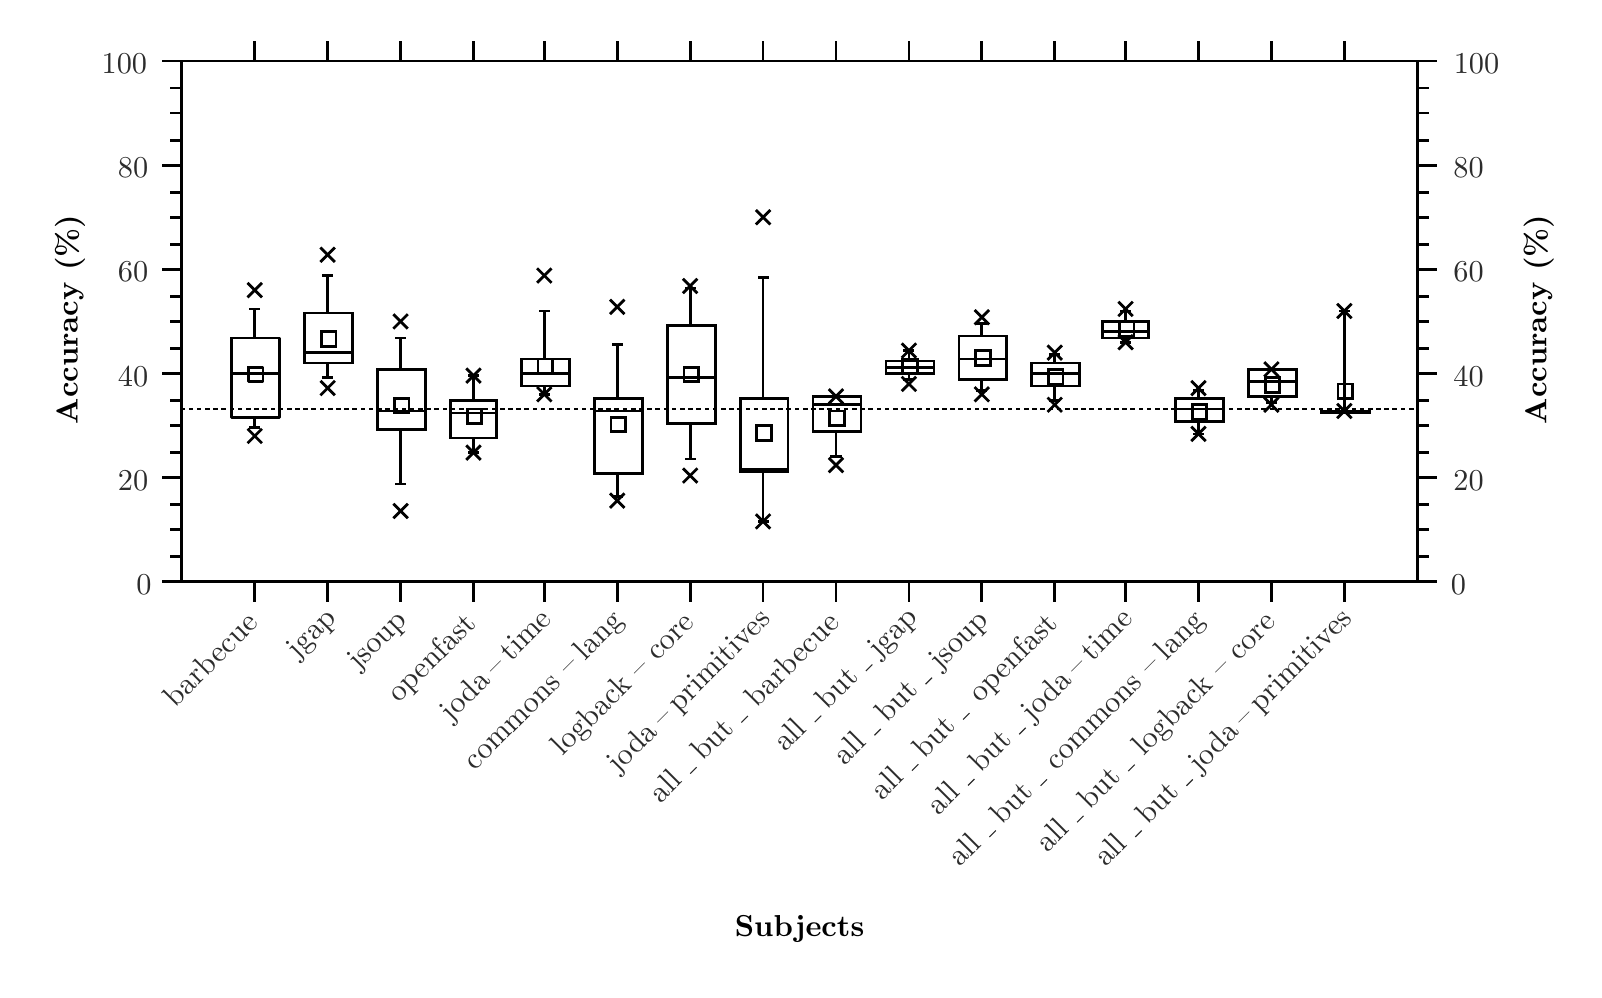
\begin{tikzpicture}{0pt}{0pt}{742pt}{452pt}
	\clip(0pt,452pt) -- (558.587pt,452pt) -- (558.587pt,111.729pt) -- (0pt,111.729pt) -- (0pt,452pt);
\begin{scope}
	\clip(55.7081pt,439.955pt) -- (502.126pt,439.955pt) -- (502.126pt,251.752pt) -- (55.7081pt,251.752pt) -- (55.7081pt,439.955pt);
	\color[rgb]{0,0,0}
	\draw[line width=1pt, line join=bevel, line cap=rect](73.7756pt,339.831pt) -- (91.0903pt,339.831pt) -- (91.0903pt,311.224pt) -- (73.7756pt,311.224pt) -- (73.7756pt,339.831pt);
	\color[rgb]{0,0,0}
	\draw[line width=1pt, line join=bevel, line cap=rect](80.5509pt,307.46pt) -- (83.5622pt,307.46pt);
	\draw[line width=1pt, line join=bevel, line cap=rect](80.5509pt,350.37pt) -- (83.5622pt,350.37pt);
	\draw[line width=1pt, line join=bevel, line cap=rect](82.0566pt,350.37pt) -- (82.0566pt,339.831pt);
	\draw[line width=1pt, line join=bevel, line cap=rect](82.0566pt,307.46pt) -- (82.0566pt,311.224pt);
	\draw[line width=1pt, line join=bevel, line cap=rect](73.7756pt,327.033pt) -- (90.3375pt,327.033pt);
	\draw[line width=1pt, line join=bevel, line cap=rect](79.7981pt,306.707pt) -- (84.315pt,302.19pt);
	\draw[line width=1pt, line join=bevel, line cap=rect](79.7981pt,302.19pt) -- (84.315pt,306.707pt);
	\draw[line width=1pt, line join=bevel, line cap=rect](79.7981pt,359.404pt) -- (84.315pt,354.887pt);
	\draw[line width=1pt, line join=bevel, line cap=rect](79.7981pt,354.887pt) -- (84.315pt,359.404pt);
	\draw[line width=1pt, line join=bevel, line cap=rect](79.7981pt,329.292pt) -- (85.0678pt,329.292pt) -- (85.0678pt,324.022pt) -- (79.7981pt,324.022pt) -- (79.7981pt,329.292pt);
	\draw[line width=1pt, line join=miter, line cap=rect](100.124pt,348.865pt) -- (117.439pt,348.865pt) -- (117.439pt,330.797pt) -- (100.124pt,330.797pt) -- (100.124pt,348.865pt);
	\draw[line width=1pt, line join=miter, line cap=rect](106.899pt,325.528pt) -- (109.911pt,325.528pt);
	\draw[line width=1pt, line join=miter, line cap=rect](106.899pt,362.415pt) -- (109.911pt,362.415pt);
	\draw[line width=1pt, line join=miter, line cap=rect](108.405pt,362.415pt) -- (108.405pt,348.865pt);
	\draw[line width=1pt, line join=miter, line cap=rect](108.405pt,325.528pt) -- (108.405pt,330.797pt);
	\draw[line width=1pt, line join=miter, line cap=rect](100.124pt,334.561pt) -- (116.686pt,334.561pt);
	\draw[line width=1pt, line join=miter, line cap=rect](106.147pt,324.022pt) -- (110.663pt,319.505pt);
	\draw[line width=1pt, line join=miter, line cap=rect](106.147pt,319.505pt) -- (110.663pt,324.022pt);
	\draw[line width=1pt, line join=miter, line cap=rect](106.147pt,372.202pt) -- (110.663pt,367.685pt);
	\draw[line width=1pt, line join=miter, line cap=rect](106.147pt,367.685pt) -- (110.663pt,372.202pt);
	\draw[line width=1pt, line join=miter, line cap=rect](106.147pt,342.089pt) -- (111.416pt,342.089pt) -- (111.416pt,336.82pt) -- (106.147pt,336.82pt) -- (106.147pt,342.089pt);
	\draw[line width=1pt, line join=miter, line cap=rect](126.472pt,328.539pt) -- (143.787pt,328.539pt) -- (143.787pt,306.707pt) -- (126.472pt,306.707pt) -- (126.472pt,328.539pt);
	\draw[line width=1pt, line join=miter, line cap=rect](133.248pt,287.134pt) -- (136.259pt,287.134pt);
	\draw[line width=1pt, line join=miter, line cap=rect](133.248pt,339.831pt) -- (136.259pt,339.831pt);
	\draw[line width=1pt, line join=miter, line cap=rect](134.753pt,339.831pt) -- (134.753pt,328.539pt);
	\draw[line width=1pt, line join=miter, line cap=rect](134.753pt,287.134pt) -- (134.753pt,306.707pt);
	\draw[line width=1pt, line join=miter, line cap=rect](126.472pt,313.482pt) -- (143.034pt,313.482pt);
	\draw[line width=1pt, line join=miter, line cap=rect](132.495pt,279.606pt) -- (137.012pt,275.089pt);
	\draw[line width=1pt, line join=miter, line cap=rect](132.495pt,275.089pt) -- (137.012pt,279.606pt);
	\draw[line width=1pt, line join=miter, line cap=rect](132.495pt,348.112pt) -- (137.012pt,343.595pt);
	\draw[line width=1pt, line join=miter, line cap=rect](132.495pt,343.595pt) -- (137.012pt,348.112pt);
	\draw[line width=1pt, line join=miter, line cap=rect](132.495pt,317.999pt) -- (137.765pt,317.999pt) -- (137.765pt,312.73pt) -- (132.495pt,312.73pt) -- (132.495pt,317.999pt);
	\draw[line width=1pt, line join=miter, line cap=rect](152.821pt,317.247pt) -- (169.383pt,317.247pt) -- (169.383pt,303.696pt) -- (152.821pt,303.696pt) -- (152.821pt,317.247pt);
	\draw[line width=1pt, line join=miter, line cap=rect](159.596pt,298.426pt) -- (162.607pt,298.426pt);
	\draw[line width=1pt, line join=miter, line cap=rect](159.596pt,326.28pt) -- (162.607pt,326.28pt);
	\draw[line width=1pt, line join=miter, line cap=rect](161.102pt,326.28pt) -- (161.102pt,317.247pt);
	\draw[line width=1pt, line join=miter, line cap=rect](161.102pt,298.426pt) -- (161.102pt,303.696pt);
	\draw[line width=1pt, line join=miter, line cap=rect](152.821pt,312.73pt) -- (169.383pt,312.73pt);
	\draw[line width=1pt, line join=miter, line cap=rect](158.843pt,300.685pt) -- (163.36pt,296.168pt);
	\draw[line width=1pt, line join=miter, line cap=rect](158.843pt,296.168pt) -- (163.36pt,300.685pt);
	\draw[line width=1pt, line join=miter, line cap=rect](158.843pt,328.539pt) -- (163.36pt,324.022pt);
	\draw[line width=1pt, line join=miter, line cap=rect](158.843pt,324.022pt) -- (163.36pt,328.539pt);
	\draw[line width=1pt, line join=miter, line cap=rect](158.843pt,314.235pt) -- (164.113pt,314.235pt) -- (164.113pt,308.966pt) -- (158.843pt,308.966pt) -- (158.843pt,314.235pt);
	\draw[line width=1pt, line join=miter, line cap=rect](178.417pt,332.303pt) -- (195.731pt,332.303pt) -- (195.731pt,322.516pt) -- (178.417pt,322.516pt) -- (178.417pt,332.303pt);
	\draw[line width=1pt, line join=miter, line cap=rect](185.192pt,319.505pt) -- (188.203pt,319.505pt);
	\draw[line width=1pt, line join=miter, line cap=rect](185.192pt,349.618pt) -- (188.203pt,349.618pt);
	\draw[line width=1pt, line join=miter, line cap=rect](186.697pt,349.618pt) -- (186.697pt,332.303pt);
	\draw[line width=1pt, line join=miter, line cap=rect](186.697pt,319.505pt) -- (186.697pt,322.516pt);
	\draw[line width=1pt, line join=miter, line cap=rect](178.417pt,327.033pt) -- (194.978pt,327.033pt);
	\draw[line width=1pt, line join=miter, line cap=rect](184.439pt,321.763pt) -- (188.956pt,317.247pt);
	\draw[line width=1pt, line join=miter, line cap=rect](184.439pt,317.247pt) -- (188.956pt,321.763pt);
	\draw[line width=1pt, line join=miter, line cap=rect](184.439pt,364.674pt) -- (188.956pt,360.157pt);
	\draw[line width=1pt, line join=miter, line cap=rect](184.439pt,360.157pt) -- (188.956pt,364.674pt);
	\draw[line width=1pt, line join=miter, line cap=rect](184.439pt,332.303pt) -- (189.709pt,332.303pt) -- (189.709pt,327.033pt) -- (184.439pt,327.033pt) -- (184.439pt,332.303pt);
	\draw[line width=1pt, line join=miter, line cap=rect](204.765pt,317.999pt) -- (222.08pt,317.999pt) -- (222.08pt,290.898pt) -- (204.765pt,290.898pt) -- (204.765pt,317.999pt);
	\draw[line width=1pt, line join=miter, line cap=rect](211.54pt,282.617pt) -- (214.552pt,282.617pt);
	\draw[line width=1pt, line join=miter, line cap=rect](211.54pt,337.572pt) -- (214.552pt,337.572pt);
	\draw[line width=1pt, line join=miter, line cap=rect](213.046pt,337.572pt) -- (213.046pt,317.999pt);
	\draw[line width=1pt, line join=miter, line cap=rect](213.046pt,282.617pt) -- (213.046pt,290.898pt);
	\draw[line width=1pt, line join=miter, line cap=rect](204.765pt,313.482pt) -- (221.327pt,313.482pt);
	\draw[line width=1pt, line join=miter, line cap=rect](210.787pt,283.37pt) -- (215.304pt,278.853pt);
	\draw[line width=1pt, line join=miter, line cap=rect](210.787pt,278.853pt) -- (215.304pt,283.37pt);
	\draw[line width=1pt, line join=miter, line cap=rect](210.787pt,353.382pt) -- (215.304pt,348.865pt);
	\draw[line width=1pt, line join=miter, line cap=rect](210.787pt,348.865pt) -- (215.304pt,353.382pt);
	\draw[line width=1pt, line join=miter, line cap=rect](210.787pt,311.224pt) -- (216.057pt,311.224pt) -- (216.057pt,305.954pt) -- (210.787pt,305.954pt) -- (210.787pt,311.224pt);
	\draw[line width=1pt, line join=miter, line cap=rect](231.113pt,344.348pt) -- (248.428pt,344.348pt) -- (248.428pt,308.966pt) -- (231.113pt,308.966pt) -- (231.113pt,344.348pt);
	\draw[line width=1pt, line join=miter, line cap=rect](237.889pt,296.168pt) -- (240.9pt,296.168pt);
	\draw[line width=1pt, line join=miter, line cap=rect](237.889pt,357.898pt) -- (240.9pt,357.898pt);
	\draw[line width=1pt, line join=miter, line cap=rect](239.394pt,357.898pt) -- (239.394pt,344.348pt);
	\draw[line width=1pt, line join=miter, line cap=rect](239.394pt,296.168pt) -- (239.394pt,308.966pt);
	\draw[line width=1pt, line join=miter, line cap=rect](231.113pt,325.528pt) -- (247.675pt,325.528pt);
	\draw[line width=1pt, line join=miter, line cap=rect](237.136pt,292.404pt) -- (241.653pt,287.887pt);
	\draw[line width=1pt, line join=miter, line cap=rect](237.136pt,287.887pt) -- (241.653pt,292.404pt);
	\draw[line width=1pt, line join=miter, line cap=rect](237.136pt,360.91pt) -- (241.653pt,356.393pt);
	\draw[line width=1pt, line join=miter, line cap=rect](237.136pt,356.393pt) -- (241.653pt,360.91pt);
	\draw[line width=1pt, line join=miter, line cap=rect](237.136pt,329.292pt) -- (242.406pt,329.292pt) -- (242.406pt,324.022pt) -- (237.136pt,324.022pt) -- (237.136pt,329.292pt);
	\draw[line width=1pt, line join=miter, line cap=rect](257.462pt,317.999pt) -- (274.777pt,317.999pt) -- (274.777pt,291.651pt) -- (257.462pt,291.651pt) -- (257.462pt,317.999pt);
	\draw[line width=1pt, line join=miter, line cap=rect](264.237pt,273.583pt) -- (267.248pt,273.583pt);
	\draw[line width=1pt, line join=miter, line cap=rect](264.237pt,361.663pt) -- (267.248pt,361.663pt);
	\draw[line width=1pt, line join=miter, line cap=rect](265.743pt,361.663pt) -- (265.743pt,317.999pt);
	\draw[line width=1pt, line join=miter, line cap=rect](265.743pt,273.583pt) -- (265.743pt,291.651pt);
	\draw[line width=1pt, line join=miter, line cap=rect](257.462pt,292.404pt) -- (274.024pt,292.404pt);
	\draw[line width=1pt, line join=miter, line cap=rect](263.484pt,275.842pt) -- (268.001pt,271.325pt);
	\draw[line width=1pt, line join=miter, line cap=rect](263.484pt,271.325pt) -- (268.001pt,275.842pt);
	\draw[line width=1pt, line join=miter, line cap=rect](263.484pt,385.752pt) -- (268.001pt,381.236pt);
	\draw[line width=1pt, line join=miter, line cap=rect](263.484pt,381.236pt) -- (268.001pt,385.752pt);
	\draw[line width=1pt, line join=miter, line cap=rect](263.484pt,308.213pt) -- (268.754pt,308.213pt) -- (268.754pt,302.943pt) -- (263.484pt,302.943pt) -- (263.484pt,308.213pt);
	\draw[line width=1pt, line join=miter, line cap=rect](283.81pt,318.752pt) -- (301.125pt,318.752pt) -- (301.125pt,305.954pt) -- (283.81pt,305.954pt) -- (283.81pt,318.752pt);
	\draw[line width=1pt, line join=miter, line cap=rect](290.586pt,296.921pt) -- (293.597pt,296.921pt);
	\draw[line width=1pt, line join=miter, line cap=rect](290.586pt,318.752pt) -- (293.597pt,318.752pt);
	\draw[line width=1pt, line join=miter, line cap=rect](292.091pt,296.921pt) -- (292.091pt,305.954pt);
	\draw[line width=1pt, line join=miter, line cap=rect](283.81pt,315.741pt) -- (300.372pt,315.741pt);
	\draw[line width=1pt, line join=miter, line cap=rect](289.833pt,296.168pt) -- (294.35pt,291.651pt);
	\draw[line width=1pt, line join=miter, line cap=rect](289.833pt,291.651pt) -- (294.35pt,296.168pt);
	\draw[line width=1pt, line join=miter, line cap=rect](289.833pt,321.011pt) -- (294.35pt,316.494pt);
	\draw[line width=1pt, line join=miter, line cap=rect](289.833pt,316.494pt) -- (294.35pt,321.011pt);
	\draw[line width=1pt, line join=miter, line cap=rect](289.833pt,313.482pt) -- (295.103pt,313.482pt) -- (295.103pt,308.213pt) -- (289.833pt,308.213pt) -- (289.833pt,313.482pt);
	\draw[line width=1pt, line join=miter, line cap=rect](310.159pt,331.55pt) -- (327.473pt,331.55pt) -- (327.473pt,327.033pt) -- (310.159pt,327.033pt) -- (310.159pt,331.55pt);
	\draw[line width=1pt, line join=miter, line cap=rect](316.934pt,324.775pt) -- (319.945pt,324.775pt);
	\draw[line width=1pt, line join=miter, line cap=rect](316.934pt,335.314pt) -- (319.945pt,335.314pt);
	\draw[line width=1pt, line join=miter, line cap=rect](318.44pt,335.314pt) -- (318.44pt,331.55pt);
	\draw[line width=1pt, line join=miter, line cap=rect](318.44pt,324.775pt) -- (318.44pt,327.033pt);
	\draw[line width=1pt, line join=miter, line cap=rect](310.159pt,329.292pt) -- (326.721pt,329.292pt);
	\draw[line width=1pt, line join=miter, line cap=rect](316.181pt,325.528pt) -- (320.698pt,321.011pt);
	\draw[line width=1pt, line join=miter, line cap=rect](316.181pt,321.011pt) -- (320.698pt,325.528pt);
	\draw[line width=1pt, line join=miter, line cap=rect](316.181pt,337.572pt) -- (320.698pt,333.056pt);
	\draw[line width=1pt, line join=miter, line cap=rect](316.181pt,333.056pt) -- (320.698pt,337.572pt);
	\draw[line width=1pt, line join=miter, line cap=rect](316.181pt,332.303pt) -- (321.451pt,332.303pt) -- (321.451pt,327.033pt) -- (316.181pt,327.033pt) -- (316.181pt,332.303pt);
	\draw[line width=1pt, line join=miter, line cap=rect](336.507pt,340.584pt) -- (353.822pt,340.584pt) -- (353.822pt,324.775pt) -- (336.507pt,324.775pt) -- (336.507pt,340.584pt);
	\draw[line width=1pt, line join=miter, line cap=rect](343.282pt,321.011pt) -- (346.294pt,321.011pt);
	\draw[line width=1pt, line join=miter, line cap=rect](343.282pt,345.101pt) -- (346.294pt,345.101pt);
	\draw[line width=1pt, line join=miter, line cap=rect](344.788pt,345.101pt) -- (344.788pt,340.584pt);
	\draw[line width=1pt, line join=miter, line cap=rect](344.788pt,321.011pt) -- (344.788pt,324.775pt);
	\draw[line width=1pt, line join=miter, line cap=rect](336.507pt,332.303pt) -- (353.069pt,332.303pt);
	\draw[line width=1pt, line join=miter, line cap=rect](342.53pt,321.763pt) -- (347.047pt,317.247pt);
	\draw[line width=1pt, line join=miter, line cap=rect](342.53pt,317.247pt) -- (347.047pt,321.763pt);
	\draw[line width=1pt, line join=miter, line cap=rect](342.53pt,349.618pt) -- (347.047pt,345.101pt);
	\draw[line width=1pt, line join=miter, line cap=rect](342.53pt,345.101pt) -- (347.047pt,349.618pt);
	\draw[line width=1pt, line join=miter, line cap=rect](342.53pt,335.314pt) -- (347.799pt,335.314pt) -- (347.799pt,330.044pt) -- (342.53pt,330.044pt) -- (342.53pt,335.314pt);
	\draw[line width=1pt, line join=miter, line cap=rect](362.856pt,330.797pt) -- (380.17pt,330.797pt) -- (380.17pt,322.516pt) -- (362.856pt,322.516pt) -- (362.856pt,330.797pt);
	\draw[line width=1pt, line join=miter, line cap=rect](369.631pt,317.247pt) -- (372.642pt,317.247pt);
	\draw[line width=1pt, line join=miter, line cap=rect](369.631pt,333.808pt) -- (372.642pt,333.808pt);
	\draw[line width=1pt, line join=miter, line cap=rect](371.137pt,333.808pt) -- (371.137pt,330.797pt);
	\draw[line width=1pt, line join=miter, line cap=rect](371.137pt,317.247pt) -- (371.137pt,322.516pt);
	\draw[line width=1pt, line join=miter, line cap=rect](362.856pt,327.033pt) -- (379.418pt,327.033pt);
	\draw[line width=1pt, line join=miter, line cap=rect](368.878pt,317.999pt) -- (373.395pt,313.482pt);
	\draw[line width=1pt, line join=miter, line cap=rect](368.878pt,313.482pt) -- (373.395pt,317.999pt);
	\draw[line width=1pt, line join=miter, line cap=rect](368.878pt,336.82pt) -- (373.395pt,332.303pt);
	\draw[line width=1pt, line join=miter, line cap=rect](368.878pt,332.303pt) -- (373.395pt,336.82pt);
	\draw[line width=1pt, line join=miter, line cap=rect](368.878pt,328.539pt) -- (374.148pt,328.539pt) -- (374.148pt,323.269pt) -- (368.878pt,323.269pt) -- (368.878pt,328.539pt);
	\draw[line width=1pt, line join=miter, line cap=rect](388.451pt,345.853pt) -- (405.013pt,345.853pt) -- (405.013pt,339.831pt) -- (388.451pt,339.831pt) -- (388.451pt,345.853pt);
	\draw[line width=1pt, line join=miter, line cap=rect](395.227pt,338.325pt) -- (398.238pt,338.325pt);
	\draw[line width=1pt, line join=miter, line cap=rect](395.227pt,349.618pt) -- (398.238pt,349.618pt);
	\draw[line width=1pt, line join=miter, line cap=rect](396.732pt,349.618pt) -- (396.732pt,345.853pt);
	\draw[line width=1pt, line join=miter, line cap=rect](396.732pt,338.325pt) -- (396.732pt,339.831pt);
	\draw[line width=1pt, line join=miter, line cap=rect](388.451pt,342.089pt) -- (405.013pt,342.089pt);
	\draw[line width=1pt, line join=miter, line cap=rect](394.474pt,340.584pt) -- (398.991pt,336.067pt);
	\draw[line width=1pt, line join=miter, line cap=rect](394.474pt,336.067pt) -- (398.991pt,340.584pt);
	\draw[line width=1pt, line join=miter, line cap=rect](394.474pt,352.629pt) -- (398.991pt,348.112pt);
	\draw[line width=1pt, line join=miter, line cap=rect](394.474pt,348.112pt) -- (398.991pt,352.629pt);
	\draw[line width=1pt, line join=miter, line cap=rect](394.474pt,345.853pt) -- (399.743pt,345.853pt) -- (399.743pt,340.584pt) -- (394.474pt,340.584pt) -- (394.474pt,345.853pt);
	\draw[line width=1pt, line join=miter, line cap=rect](414.8pt,317.999pt) -- (432.114pt,317.999pt) -- (432.114pt,309.718pt) -- (414.8pt,309.718pt) -- (414.8pt,317.999pt);
	\draw[line width=1pt, line join=miter, line cap=rect](421.575pt,305.202pt) -- (424.586pt,305.202pt);
	\draw[line width=1pt, line join=miter, line cap=rect](421.575pt,321.011pt) -- (424.586pt,321.011pt);
	\draw[line width=1pt, line join=miter, line cap=rect](423.081pt,321.011pt) -- (423.081pt,317.999pt);
	\draw[line width=1pt, line join=miter, line cap=rect](423.081pt,305.202pt) -- (423.081pt,309.718pt);
	\draw[line width=1pt, line join=miter, line cap=rect](414.8pt,314.235pt) -- (431.362pt,314.235pt);
	\draw[line width=1pt, line join=miter, line cap=rect](420.822pt,307.46pt) -- (425.339pt,302.943pt);
	\draw[line width=1pt, line join=miter, line cap=rect](420.822pt,302.943pt) -- (425.339pt,307.46pt);
	\draw[line width=1pt, line join=miter, line cap=rect](420.822pt,324.022pt) -- (425.339pt,319.505pt);
	\draw[line width=1pt, line join=miter, line cap=rect](420.822pt,319.505pt) -- (425.339pt,324.022pt);
	\draw[line width=1pt, line join=miter, line cap=rect](420.822pt,315.741pt) -- (426.092pt,315.741pt) -- (426.092pt,310.471pt) -- (420.822pt,310.471pt) -- (420.822pt,315.741pt);
	\draw[line width=1pt, line join=miter, line cap=rect](441.148pt,328.539pt) -- (458.463pt,328.539pt) -- (458.463pt,318.752pt) -- (441.148pt,318.752pt) -- (441.148pt,328.539pt);
	\draw[line width=1pt, line join=miter, line cap=rect](447.923pt,316.494pt) -- (450.935pt,316.494pt);
	\draw[line width=1pt, line join=miter, line cap=rect](447.923pt,328.539pt) -- (450.935pt,328.539pt);
	\draw[line width=1pt, line join=miter, line cap=rect](449.429pt,316.494pt) -- (449.429pt,318.752pt);
	\draw[line width=1pt, line join=miter, line cap=rect](441.148pt,324.022pt) -- (457.71pt,324.022pt);
	\draw[line width=1pt, line join=miter, line cap=rect](447.171pt,317.999pt) -- (451.688pt,313.482pt);
	\draw[line width=1pt, line join=miter, line cap=rect](447.171pt,313.482pt) -- (451.688pt,317.999pt);
	\draw[line width=1pt, line join=miter, line cap=rect](447.171pt,330.797pt) -- (451.688pt,326.28pt);
	\draw[line width=1pt, line join=miter, line cap=rect](447.171pt,326.28pt) -- (451.688pt,330.797pt);
	\draw[line width=1pt, line join=miter, line cap=rect](447.171pt,325.528pt) -- (452.44pt,325.528pt) -- (452.44pt,320.258pt) -- (447.171pt,320.258pt) -- (447.171pt,325.528pt);
	\draw[line width=1pt, line join=miter, line cap=rect](467.497pt,313.482pt) -- (484.811pt,313.482pt) -- (484.811pt,312.73pt) -- (467.497pt,312.73pt) -- (467.497pt,313.482pt);
	\draw[line width=1pt, line join=miter, line cap=rect](474.272pt,313.482pt) -- (477.283pt,313.482pt);
	\draw[line width=1pt, line join=miter, line cap=rect](474.272pt,349.618pt) -- (477.283pt,349.618pt);
	\draw[line width=1pt, line join=miter, line cap=rect](475.777pt,349.618pt) -- (475.777pt,313.482pt);
	\draw[line width=1pt, line join=miter, line cap=rect](467.497pt,313.482pt) -- (484.058pt,313.482pt);
	\draw[line width=1pt, line join=miter, line cap=rect](473.519pt,315.741pt) -- (478.036pt,311.224pt);
	\draw[line width=1pt, line join=miter, line cap=rect](473.519pt,311.224pt) -- (478.036pt,315.741pt);
	\draw[line width=1pt, line join=miter, line cap=rect](473.519pt,351.876pt) -- (478.036pt,347.359pt);
	\draw[line width=1pt, line join=miter, line cap=rect](473.519pt,347.359pt) -- (478.036pt,351.876pt);
	\draw[line width=1pt, line join=miter, line cap=rect](473.519pt,323.269pt) -- (478.789pt,323.269pt) -- (478.789pt,317.999pt) -- (473.519pt,317.999pt) -- (473.519pt,323.269pt);
	\draw[line width=1pt, dash pattern=on 0.024cm off 0.08cm, dash phase=0pt, line join=miter, line cap=rect](55.7081pt,314.235pt) -- (528.474pt,314.235pt);
\end{scope}
\begin{scope}
	\color[rgb]{0,0,0}
	\pgftext[center, base, at={\pgfpoint{18.0675pt}{346.606pt}},rotate=90]{\fontsize{11}{0}\selectfont{\textbf{Accuracy (\%)}}}
	\color[rgb]{0.172549,0.172549,0.172549}
	\pgftext[center, base, at={\pgfpoint{42.0163pt}{247.235pt}}]{\fontsize{11}{0}\selectfont{0}}
	\pgftext[center, base, at={\pgfpoint{38.1111pt}{284.876pt}}]{\fontsize{11}{0}\selectfont{20}}
	\pgftext[center, base, at={\pgfpoint{38.1111pt}{322.516pt}}]{\fontsize{11}{0}\selectfont{40}}
	\pgftext[center, base, at={\pgfpoint{38.1111pt}{360.157pt}}]{\fontsize{11}{0}\selectfont{60}}
	\pgftext[center, base, at={\pgfpoint{38.1111pt}{397.798pt}}]{\fontsize{11}{0}\selectfont{80}}
	\pgftext[center, base, at={\pgfpoint{34.9587pt}{435.438pt}}]{\fontsize{11}{0}\selectfont{100}}
	\color[rgb]{0,0,0}
	\draw[line width=1pt, line join=bevel, line cap=rect](55.7081pt,260.786pt) -- (51.9441pt,260.786pt);
	\draw[line width=1pt, line join=bevel, line cap=rect](55.7081pt,279.606pt) -- (51.9441pt,279.606pt);
	\draw[line width=1pt, line join=bevel, line cap=rect](55.7081pt,298.426pt) -- (51.9441pt,298.426pt);
	\draw[line width=1pt, line join=bevel, line cap=rect](55.7081pt,317.247pt) -- (51.9441pt,317.247pt);
	\draw[line width=1pt, line join=bevel, line cap=rect](55.7081pt,336.067pt) -- (51.9441pt,336.067pt);
	\draw[line width=1pt, line join=bevel, line cap=rect](55.7081pt,354.887pt) -- (51.9441pt,354.887pt);
	\draw[line width=1pt, line join=bevel, line cap=rect](55.7081pt,373.707pt) -- (51.9441pt,373.707pt);
	\draw[line width=1pt, line join=bevel, line cap=rect](55.7081pt,392.528pt) -- (51.9441pt,392.528pt);
	\draw[line width=1pt, line join=bevel, line cap=rect](55.7081pt,411.348pt) -- (51.9441pt,411.348pt);
	\draw[line width=1pt, line join=bevel, line cap=rect](55.7081pt,430.168pt) -- (51.9441pt,430.168pt);
	\draw[line width=1pt, line join=bevel, line cap=rect](55.7081pt,270.572pt) -- (51.9441pt,270.572pt);
	\draw[line width=1pt, line join=bevel, line cap=rect](55.7081pt,308.213pt) -- (51.9441pt,308.213pt);
	\draw[line width=1pt, line join=bevel, line cap=rect](55.7081pt,345.853pt) -- (51.9441pt,345.853pt);
	\draw[line width=1pt, line join=bevel, line cap=rect](55.7081pt,383.494pt) -- (51.9441pt,383.494pt);
	\draw[line width=1pt, line join=bevel, line cap=rect](55.7081pt,421.135pt) -- (51.9441pt,421.135pt);
	\draw[line width=1pt, line join=bevel, line cap=rect](55.7081pt,251.752pt) -- (48.9328pt,251.752pt);
	\draw[line width=1pt, line join=bevel, line cap=rect](55.7081pt,289.393pt) -- (48.9328pt,289.393pt);
	\draw[line width=1pt, line join=bevel, line cap=rect](55.7081pt,327.033pt) -- (48.9328pt,327.033pt);
	\draw[line width=1pt, line join=bevel, line cap=rect](55.7081pt,364.674pt) -- (48.9328pt,364.674pt);
	\draw[line width=1pt, line join=bevel, line cap=rect](55.7081pt,402.314pt) -- (48.9328pt,402.314pt);
	\draw[line width=1pt, line join=bevel, line cap=rect](55.7081pt,439.955pt) -- (48.9328pt,439.955pt);
	\draw[line width=1pt, line join=bevel, line cap=rect](55.7081pt,439.955pt) -- (55.7081pt,251.752pt);
	\pgftext[center, base, at={\pgfpoint{548.8pt}{346.606pt}},rotate=90]{\fontsize{11}{0}\selectfont{\textbf{Accuracy (\%)}}}
	\color[rgb]{0.172549,0.172549,0.172549}
	\pgftext[center, base, at={\pgfpoint{517.041pt}{247.235pt}}]{\fontsize{11}{0}\selectfont{0}}
	\pgftext[center, base, at={\pgfpoint{520.664pt}{284.876pt}}]{\fontsize{11}{0}\selectfont{20}}
	\pgftext[center, base, at={\pgfpoint{520.664pt}{322.516pt}}]{\fontsize{11}{0}\selectfont{40}}
	\pgftext[center, base, at={\pgfpoint{520.664pt}{360.157pt}}]{\fontsize{11}{0}\selectfont{60}}
	\pgftext[center, base, at={\pgfpoint{520.664pt}{397.798pt}}]{\fontsize{11}{0}\selectfont{80}}
	\pgftext[center, base, at={\pgfpoint{523.534pt}{435.438pt}}]{\fontsize{11}{0}\selectfont{100}}
	\color[rgb]{0,0,0}
	\draw[line width=1pt, line join=bevel, line cap=rect](502.126pt,260.786pt) -- (505.89pt,260.786pt);
	\draw[line width=1pt, line join=bevel, line cap=rect](502.126pt,279.606pt) -- (505.89pt,279.606pt);
	\draw[line width=1pt, line join=bevel, line cap=rect](502.126pt,298.426pt) -- (505.89pt,298.426pt);
	\draw[line width=1pt, line join=bevel, line cap=rect](502.126pt,317.247pt) -- (505.89pt,317.247pt);
	\draw[line width=1pt, line join=bevel, line cap=rect](502.126pt,336.067pt) -- (505.89pt,336.067pt);
	\draw[line width=1pt, line join=bevel, line cap=rect](502.126pt,354.887pt) -- (505.89pt,354.887pt);
	\draw[line width=1pt, line join=bevel, line cap=rect](502.126pt,373.707pt) -- (505.89pt,373.707pt);
	\draw[line width=1pt, line join=bevel, line cap=rect](502.126pt,392.528pt) -- (505.89pt,392.528pt);
	\draw[line width=1pt, line join=bevel, line cap=rect](502.126pt,411.348pt) -- (505.89pt,411.348pt);
	\draw[line width=1pt, line join=bevel, line cap=rect](502.126pt,430.168pt) -- (505.89pt,430.168pt);
	\draw[line width=1pt, line join=bevel, line cap=rect](502.126pt,270.572pt) -- (505.89pt,270.572pt);
	\draw[line width=1pt, line join=bevel, line cap=rect](502.126pt,308.213pt) -- (505.89pt,308.213pt);
	\draw[line width=1pt, line join=bevel, line cap=rect](502.126pt,345.853pt) -- (505.89pt,345.853pt);
	\draw[line width=1pt, line join=bevel, line cap=rect](502.126pt,383.494pt) -- (505.89pt,383.494pt);
	\draw[line width=1pt, line join=bevel, line cap=rect](502.126pt,421.135pt) -- (505.89pt,421.135pt);
	\draw[line width=1pt, line join=bevel, line cap=rect](502.126pt,251.752pt) -- (508.901pt,251.752pt);
	\draw[line width=1pt, line join=bevel, line cap=rect](502.126pt,289.393pt) -- (508.901pt,289.393pt);
	\draw[line width=1pt, line join=bevel, line cap=rect](502.126pt,327.033pt) -- (508.901pt,327.033pt);
	\draw[line width=1pt, line join=bevel, line cap=rect](502.126pt,364.674pt) -- (508.901pt,364.674pt);
	\draw[line width=1pt, line join=bevel, line cap=rect](502.126pt,402.314pt) -- (508.901pt,402.314pt);
	\draw[line width=1pt, line join=bevel, line cap=rect](502.126pt,439.955pt) -- (508.901pt,439.955pt);
	\draw[line width=1pt, line join=bevel, line cap=rect](502.126pt,439.955pt) -- (502.126pt,251.752pt);
	\pgftext[center, base, at={\pgfpoint{278.917pt}{123.774pt}}]{\fontsize{11}{0}\selectfont{\textbf{Subjects}}}
	\color[rgb]{0.172549,0.172549,0.172549}
	\pgftext[center, base, at={\pgfpoint{68.4991pt}{221.267pt}},rotate=45]{\fontsize{11}{0}\selectfont{barbecue}}
	\pgftext[center, base, at={\pgfpoint{104.654pt}{231.073pt}},rotate=45]{\fontsize{11}{0}\selectfont{jgap}}
	\pgftext[center, base, at={\pgfpoint{128.445pt}{228.516pt}},rotate=45]{\fontsize{11}{0}\selectfont{jsoup}}
	\pgftext[center, base, at={\pgfpoint{148.222pt}{221.945pt}},rotate=45]{\fontsize{11}{0}\selectfont{openfast}}
	\pgftext[center, base, at={\pgfpoint{160.198pt}{208.325pt}},rotate=45]{\fontsize{11}{0}\selectfont{joda}}
	\pgftext[center, base, at={\pgfpoint{171.111pt}{219.238pt}},rotate=45]{\fontsize{11}{0}\selectfont{--}}
	\pgftext[center, base, at={\pgfpoint{182.11pt}{230.238pt}},rotate=45]{\fontsize{11}{0}\selectfont{time}}
	\pgftext[center, base, at={\pgfpoint{177.272pt}{199.051pt}},rotate=45]{\fontsize{11}{0}\selectfont{commons}}
	\pgftext[center, base, at={\pgfpoint{197.542pt}{219.321pt}},rotate=45]{\fontsize{11}{0}\selectfont{--}}
	\pgftext[center, base, at={\pgfpoint{208.405pt}{230.184pt}},rotate=45]{\fontsize{11}{0}\selectfont{lang}}
	\pgftext[center, base, at={\pgfpoint{205.896pt}{201.326pt}},rotate=45]{\fontsize{11}{0}\selectfont{logback}}
	\pgftext[center, base, at={\pgfpoint{223.117pt}{218.547pt}},rotate=45]{\fontsize{11}{0}\selectfont{--}}
	\pgftext[center, base, at={\pgfpoint{234.342pt}{229.772pt}},rotate=45]{\fontsize{11}{0}\selectfont{core}}
	\pgftext[center, base, at={\pgfpoint{220.612pt}{189.694pt}},rotate=45]{\fontsize{11}{0}\selectfont{joda}}
	\pgftext[center, base, at={\pgfpoint{231.525pt}{200.607pt}},rotate=45]{\fontsize{11}{0}\selectfont{--}}
	\pgftext[center, base, at={\pgfpoint{252.027pt}{221.109pt}},rotate=45]{\fontsize{11}{0}\selectfont{primitives}}
	\pgftext[center, base, at={\pgfpoint{232.684pt}{175.417pt}},rotate=45]{\fontsize{11}{0}\selectfont{all}}
	\pgftext[center, base, at={\pgfpoint{240.498pt}{183.231pt}},rotate=45]{\fontsize{11}{0}\selectfont{\_}}
	\pgftext[center, base, at={\pgfpoint{249.743pt}{192.476pt}},rotate=45]{\fontsize{11}{0}\selectfont{but}}
	\pgftext[center, base, at={\pgfpoint{258.988pt}{201.721pt}},rotate=45]{\fontsize{11}{0}\selectfont{\_}}
	\pgftext[center, base, at={\pgfpoint{278.584pt}{221.317pt}},rotate=45]{\fontsize{11}{0}\selectfont{barbecue}}
	\pgftext[center, base, at={\pgfpoint{277.663pt}{194.048pt}},rotate=45]{\fontsize{11}{0}\selectfont{all}}
	\pgftext[center, base, at={\pgfpoint{285.478pt}{201.862pt}},rotate=45]{\fontsize{11}{0}\selectfont{\_}}
	\pgftext[center, base, at={\pgfpoint{294.722pt}{211.107pt}},rotate=45]{\fontsize{11}{0}\selectfont{but}}
	\pgftext[center, base, at={\pgfpoint{303.967pt}{220.352pt}},rotate=45]{\fontsize{11}{0}\selectfont{\_}}
	\pgftext[center, base, at={\pgfpoint{314.738pt}{231.123pt}},rotate=45]{\fontsize{11}{0}\selectfont{jgap}}
	\pgftext[center, base, at={\pgfpoint{299.221pt}{189.257pt}},rotate=45]{\fontsize{11}{0}\selectfont{all}}
	\pgftext[center, base, at={\pgfpoint{307.035pt}{197.072pt}},rotate=45]{\fontsize{11}{0}\selectfont{\_}}
	\pgftext[center, base, at={\pgfpoint{316.28pt}{206.317pt}},rotate=45]{\fontsize{11}{0}\selectfont{but}}
	\pgftext[center, base, at={\pgfpoint{325.525pt}{215.561pt}},rotate=45]{\fontsize{11}{0}\selectfont{\_}}
	\pgftext[center, base, at={\pgfpoint{338.529pt}{228.566pt}},rotate=45]{\fontsize{11}{0}\selectfont{jsoup}}
	\pgftext[center, base, at={\pgfpoint{312.794pt}{176.482pt}},rotate=45]{\fontsize{11}{0}\selectfont{all}}
	\pgftext[center, base, at={\pgfpoint{320.608pt}{184.296pt}},rotate=45]{\fontsize{11}{0}\selectfont{\_}}
	\pgftext[center, base, at={\pgfpoint{329.853pt}{193.541pt}},rotate=45]{\fontsize{11}{0}\selectfont{but}}
	\pgftext[center, base, at={\pgfpoint{339.098pt}{202.786pt}},rotate=45]{\fontsize{11}{0}\selectfont{\_}}
	\pgftext[center, base, at={\pgfpoint{358.307pt}{221.995pt}},rotate=45]{\fontsize{11}{0}\selectfont{openfast}}
	\pgftext[center, base, at={\pgfpoint{333.066pt}{171.159pt}},rotate=45]{\fontsize{11}{0}\selectfont{all}}
	\pgftext[center, base, at={\pgfpoint{340.88pt}{178.973pt}},rotate=45]{\fontsize{11}{0}\selectfont{\_}}
	\pgftext[center, base, at={\pgfpoint{350.125pt}{188.218pt}},rotate=45]{\fontsize{11}{0}\selectfont{but}}
	\pgftext[center, base, at={\pgfpoint{359.37pt}{197.463pt}},rotate=45]{\fontsize{11}{0}\selectfont{\_}}
	\pgftext[center, base, at={\pgfpoint{370.283pt}{208.375pt}},rotate=45]{\fontsize{11}{0}\selectfont{joda}}
	\pgftext[center, base, at={\pgfpoint{381.195pt}{219.288pt}},rotate=45]{\fontsize{11}{0}\selectfont{--}}
	\pgftext[center, base, at={\pgfpoint{392.195pt}{230.287pt}},rotate=45]{\fontsize{11}{0}\selectfont{time}}
	\pgftext[center, base, at={\pgfpoint{340.783pt}{152.527pt}},rotate=45]{\fontsize{11}{0}\selectfont{all}}
	\pgftext[center, base, at={\pgfpoint{348.598pt}{160.342pt}},rotate=45]{\fontsize{11}{0}\selectfont{\_}}
	\pgftext[center, base, at={\pgfpoint{357.842pt}{169.587pt}},rotate=45]{\fontsize{11}{0}\selectfont{but}}
	\pgftext[center, base, at={\pgfpoint{367.087pt}{178.831pt}},rotate=45]{\fontsize{11}{0}\selectfont{\_}}
	\pgftext[center, base, at={\pgfpoint{387.357pt}{199.101pt}},rotate=45]{\fontsize{11}{0}\selectfont{commons}}
	\pgftext[center, base, at={\pgfpoint{407.627pt}{219.371pt}},rotate=45]{\fontsize{11}{0}\selectfont{--}}
	\pgftext[center, base, at={\pgfpoint{418.489pt}{230.233pt}},rotate=45]{\fontsize{11}{0}\selectfont{lang}}
	\pgftext[center, base, at={\pgfpoint{372.455pt}{157.851pt}},rotate=45]{\fontsize{11}{0}\selectfont{all}}
	\pgftext[center, base, at={\pgfpoint{380.269pt}{165.665pt}},rotate=45]{\fontsize{11}{0}\selectfont{\_}}
	\pgftext[center, base, at={\pgfpoint{389.514pt}{174.91pt}},rotate=45]{\fontsize{11}{0}\selectfont{but}}
	\pgftext[center, base, at={\pgfpoint{398.759pt}{184.155pt}},rotate=45]{\fontsize{11}{0}\selectfont{\_}}
	\pgftext[center, base, at={\pgfpoint{415.98pt}{201.376pt}},rotate=45]{\fontsize{11}{0}\selectfont{logback}}
	\pgftext[center, base, at={\pgfpoint{433.202pt}{218.597pt}},rotate=45]{\fontsize{11}{0}\selectfont{--}}
	\pgftext[center, base, at={\pgfpoint{444.426pt}{229.822pt}},rotate=45]{\fontsize{11}{0}\selectfont{core}}
	\pgftext[center, base, at={\pgfpoint{393.48pt}{152.527pt}},rotate=45]{\fontsize{11}{0}\selectfont{all}}
	\pgftext[center, base, at={\pgfpoint{401.294pt}{160.342pt}},rotate=45]{\fontsize{11}{0}\selectfont{\_}}
	\pgftext[center, base, at={\pgfpoint{410.539pt}{169.587pt}},rotate=45]{\fontsize{11}{0}\selectfont{but}}
	\pgftext[center, base, at={\pgfpoint{419.784pt}{178.831pt}},rotate=45]{\fontsize{11}{0}\selectfont{\_}}
	\pgftext[center, base, at={\pgfpoint{430.697pt}{189.744pt}},rotate=45]{\fontsize{11}{0}\selectfont{joda}}
	\pgftext[center, base, at={\pgfpoint{441.609pt}{200.656pt}},rotate=45]{\fontsize{11}{0}\selectfont{--}}
	\pgftext[center, base, at={\pgfpoint{462.112pt}{221.159pt}},rotate=45]{\fontsize{11}{0}\selectfont{primitives}}
	\color[rgb]{0,0,0}
	\draw[line width=1pt, line join=bevel, line cap=rect](82.0566pt,251.752pt) -- (82.0566pt,244.977pt);
	\draw[line width=1pt, line join=bevel, line cap=rect](108.405pt,251.752pt) -- (108.405pt,244.977pt);
	\draw[line width=1pt, line join=bevel, line cap=rect](134.753pt,251.752pt) -- (134.753pt,244.977pt);
	\draw[line width=1pt, line join=bevel, line cap=rect](161.102pt,251.752pt) -- (161.102pt,244.977pt);
	\draw[line width=1pt, line join=bevel, line cap=rect](186.697pt,251.752pt) -- (186.697pt,244.977pt);
	\draw[line width=1pt, line join=bevel, line cap=rect](213.046pt,251.752pt) -- (213.046pt,244.977pt);
	\draw[line width=1pt, line join=bevel, line cap=rect](239.394pt,251.752pt) -- (239.394pt,244.977pt);
	\draw[line width=1pt, line join=bevel, line cap=rect](265.743pt,251.752pt) -- (265.743pt,244.977pt);
	\draw[line width=1pt, line join=bevel, line cap=rect](292.091pt,251.752pt) -- (292.091pt,244.977pt);
	\draw[line width=1pt, line join=bevel, line cap=rect](318.44pt,251.752pt) -- (318.44pt,244.977pt);
	\draw[line width=1pt, line join=bevel, line cap=rect](344.788pt,251.752pt) -- (344.788pt,244.977pt);
	\draw[line width=1pt, line join=bevel, line cap=rect](371.137pt,251.752pt) -- (371.137pt,244.977pt);
	\draw[line width=1pt, line join=bevel, line cap=rect](396.732pt,251.752pt) -- (396.732pt,244.977pt);
	\draw[line width=1pt, line join=bevel, line cap=rect](423.081pt,251.752pt) -- (423.081pt,244.977pt);
	\draw[line width=1pt, line join=bevel, line cap=rect](449.429pt,251.752pt) -- (449.429pt,244.977pt);
	\draw[line width=1pt, line join=bevel, line cap=rect](475.777pt,251.752pt) -- (475.777pt,244.977pt);
	\draw[line width=1pt, line join=bevel, line cap=rect](55.7081pt,251.752pt) -- (502.126pt,251.752pt);
	\draw[line width=1pt, line join=bevel, line cap=rect](82.0566pt,439.955pt) -- (82.0566pt,446.73pt);
	\draw[line width=1pt, line join=bevel, line cap=rect](108.405pt,439.955pt) -- (108.405pt,446.73pt);
	\draw[line width=1pt, line join=bevel, line cap=rect](134.753pt,439.955pt) -- (134.753pt,446.73pt);
	\draw[line width=1pt, line join=bevel, line cap=rect](161.102pt,439.955pt) -- (161.102pt,446.73pt);
	\draw[line width=1pt, line join=bevel, line cap=rect](186.697pt,439.955pt) -- (186.697pt,446.73pt);
	\draw[line width=1pt, line join=bevel, line cap=rect](213.046pt,439.955pt) -- (213.046pt,446.73pt);
	\draw[line width=1pt, line join=bevel, line cap=rect](239.394pt,439.955pt) -- (239.394pt,446.73pt);
	\draw[line width=1pt, line join=bevel, line cap=rect](265.743pt,439.955pt) -- (265.743pt,446.73pt);
	\draw[line width=1pt, line join=bevel, line cap=rect](292.091pt,439.955pt) -- (292.091pt,446.73pt);
	\draw[line width=1pt, line join=bevel, line cap=rect](318.44pt,439.955pt) -- (318.44pt,446.73pt);
	\draw[line width=1pt, line join=bevel, line cap=rect](344.788pt,439.955pt) -- (344.788pt,446.73pt);
	\draw[line width=1pt, line join=bevel, line cap=rect](371.137pt,439.955pt) -- (371.137pt,446.73pt);
	\draw[line width=1pt, line join=bevel, line cap=rect](396.732pt,439.955pt) -- (396.732pt,446.73pt);
	\draw[line width=1pt, line join=bevel, line cap=rect](423.081pt,439.955pt) -- (423.081pt,446.73pt);
	\draw[line width=1pt, line join=bevel, line cap=rect](449.429pt,439.955pt) -- (449.429pt,446.73pt);
	\draw[line width=1pt, line join=bevel, line cap=rect](475.777pt,439.955pt) -- (475.777pt,446.73pt);
	\draw[line width=1pt, line join=bevel, line cap=rect](55.7081pt,439.955pt) -- (502.126pt,439.955pt);
\end{scope}
\end{tikzpicture}

  \end{adjustbox}
  \caption{Class-level training and prediction accuracy over the eight test subjects and sets of \emph{all\_but\_<subject>} using generalized parameters [\emph{cost}=100, \emph{gamma}=0.01].}
  \vspace{2mm}
  \hrule
  \label{fig:prediction_with_parameters_class_graph}
\end{figure}

\begin{figure}[!tb]
  \centering
  \begin{adjustbox}{max size={.95\textwidth}{.95\textheight}}
    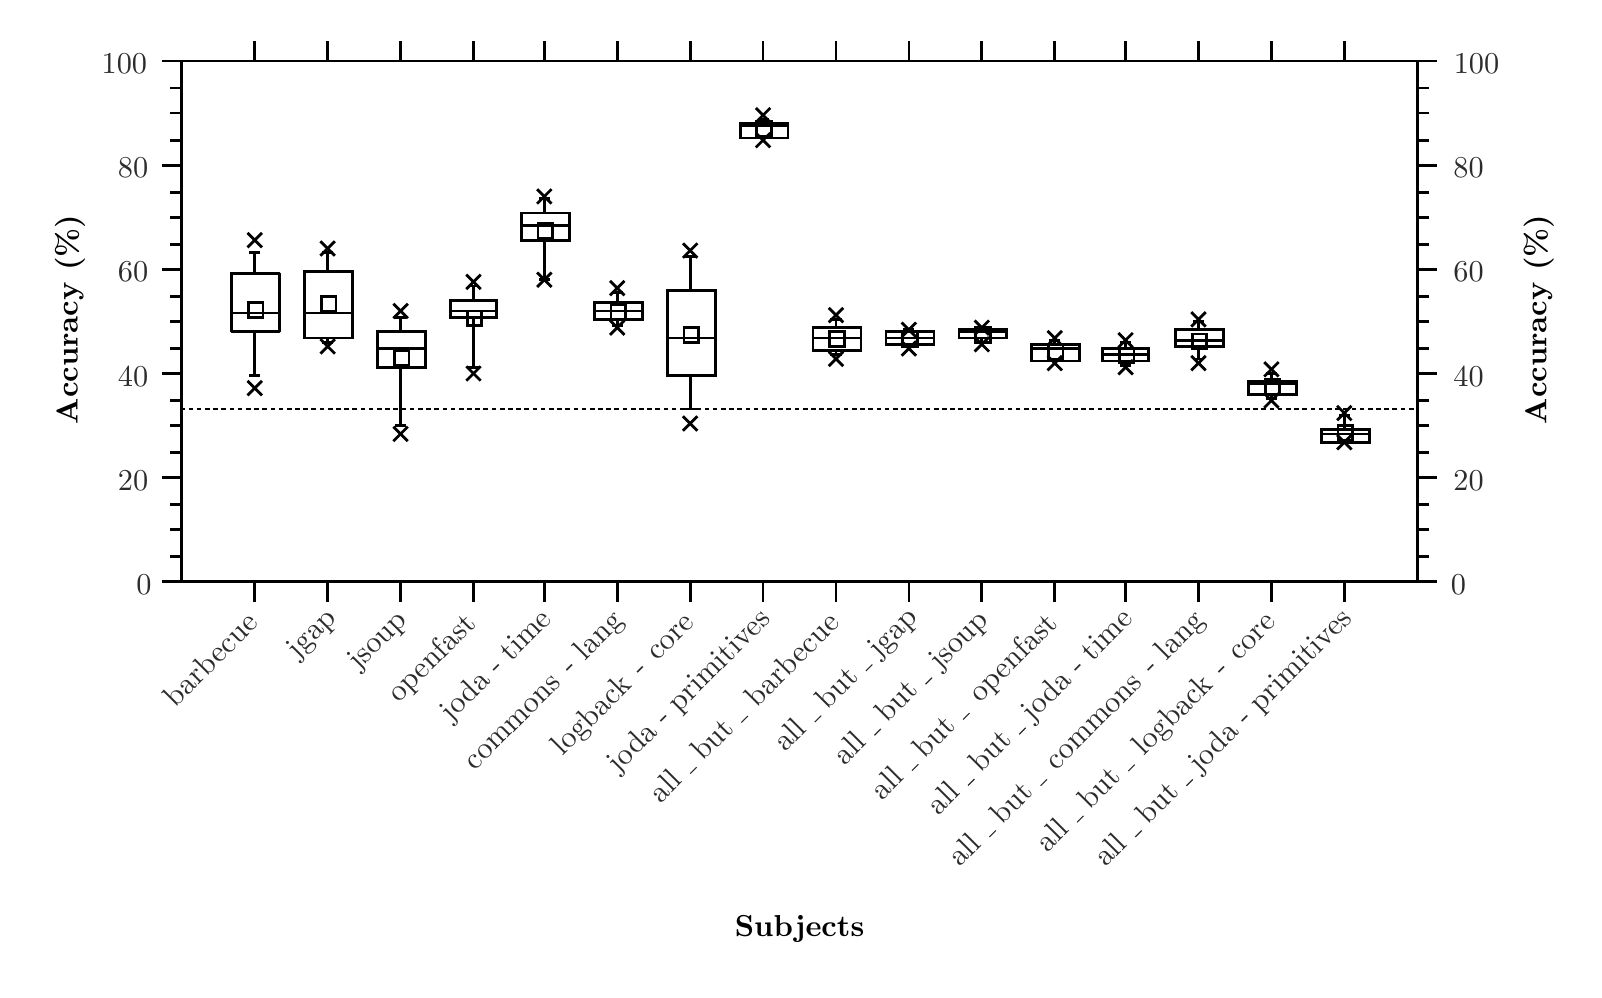
\begin{tikzpicture}{0pt}{0pt}{742pt}{452pt}
	\clip(0pt,452pt) -- (558.587pt,452pt) -- (558.587pt,111.729pt) -- (0pt,111.729pt) -- (0pt,452pt);
\begin{scope}
	\clip(55.7081pt,439.955pt) -- (502.126pt,439.955pt) -- (502.126pt,251.752pt) -- (55.7081pt,251.752pt) -- (55.7081pt,439.955pt);
	\color[rgb]{0,0,0}
	\draw[line width=1pt, line join=bevel, line cap=rect](73.7756pt,363.168pt) -- (91.0903pt,363.168pt) -- (91.0903pt,342.089pt) -- (73.7756pt,342.089pt) -- (73.7756pt,363.168pt);
	\color[rgb]{0,0,0}
	\draw[line width=1pt, line join=bevel, line cap=rect](80.5509pt,326.28pt) -- (83.5622pt,326.28pt);
	\draw[line width=1pt, line join=bevel, line cap=rect](80.5509pt,370.696pt) -- (83.5622pt,370.696pt);
	\draw[line width=1pt, line join=bevel, line cap=rect](82.0566pt,370.696pt) -- (82.0566pt,363.168pt);
	\draw[line width=1pt, line join=bevel, line cap=rect](82.0566pt,326.28pt) -- (82.0566pt,342.089pt);
	\draw[line width=1pt, line join=bevel, line cap=rect](73.7756pt,348.865pt) -- (90.3375pt,348.865pt);
	\draw[line width=1pt, line join=miter, line cap=rect](79.7981pt,324.022pt) -- (84.315pt,319.505pt);
	\draw[line width=1pt, line join=miter, line cap=rect](79.7981pt,319.505pt) -- (84.315pt,324.022pt);
	\draw[line width=1pt, line join=miter, line cap=rect](79.7981pt,377.472pt) -- (84.315pt,372.955pt);
	\draw[line width=1pt, line join=miter, line cap=rect](79.7981pt,372.955pt) -- (84.315pt,377.472pt);
	\draw[line width=1pt, line join=miter, line cap=rect](79.7981pt,352.629pt) -- (85.0678pt,352.629pt) -- (85.0678pt,347.359pt) -- (79.7981pt,347.359pt) -- (79.7981pt,352.629pt);
	\draw[line width=1pt, line join=miter, line cap=rect](100.124pt,363.921pt) -- (117.439pt,363.921pt) -- (117.439pt,339.831pt) -- (100.124pt,339.831pt) -- (100.124pt,363.921pt);
	\draw[line width=1pt, line join=miter, line cap=rect](106.899pt,338.325pt) -- (109.911pt,338.325pt);
	\draw[line width=1pt, line join=miter, line cap=rect](106.899pt,370.696pt) -- (109.911pt,370.696pt);
	\draw[line width=1pt, line join=miter, line cap=rect](108.405pt,370.696pt) -- (108.405pt,363.921pt);
	\draw[line width=1pt, line join=miter, line cap=rect](108.405pt,338.325pt) -- (108.405pt,339.831pt);
	\draw[line width=1pt, line join=miter, line cap=rect](100.124pt,348.865pt) -- (116.686pt,348.865pt);
	\draw[line width=1pt, line join=miter, line cap=rect](106.147pt,339.078pt) -- (110.663pt,334.561pt);
	\draw[line width=1pt, line join=miter, line cap=rect](106.147pt,334.561pt) -- (110.663pt,339.078pt);
	\draw[line width=1pt, line join=miter, line cap=rect](106.147pt,374.46pt) -- (110.663pt,369.943pt);
	\draw[line width=1pt, line join=miter, line cap=rect](106.147pt,369.943pt) -- (110.663pt,374.46pt);
	\draw[line width=1pt, line join=miter, line cap=rect](106.147pt,354.887pt) -- (111.416pt,354.887pt) -- (111.416pt,349.618pt) -- (106.147pt,349.618pt) -- (106.147pt,354.887pt);
	\draw[line width=1pt, line join=miter, line cap=rect](126.472pt,342.089pt) -- (143.787pt,342.089pt) -- (143.787pt,329.292pt) -- (126.472pt,329.292pt) -- (126.472pt,342.089pt);
	\draw[line width=1pt, line join=miter, line cap=rect](133.248pt,308.213pt) -- (136.259pt,308.213pt);
	\draw[line width=1pt, line join=miter, line cap=rect](133.248pt,347.359pt) -- (136.259pt,347.359pt);
	\draw[line width=1pt, line join=miter, line cap=rect](134.753pt,347.359pt) -- (134.753pt,342.089pt);
	\draw[line width=1pt, line join=miter, line cap=rect](134.753pt,308.213pt) -- (134.753pt,329.292pt);
	\draw[line width=1pt, line join=miter, line cap=rect](126.472pt,336.067pt) -- (143.034pt,336.067pt);
	\draw[line width=1pt, line join=miter, line cap=rect](132.495pt,307.46pt) -- (137.012pt,302.943pt);
	\draw[line width=1pt, line join=miter, line cap=rect](132.495pt,302.943pt) -- (137.012pt,307.46pt);
	\draw[line width=1pt, line join=miter, line cap=rect](132.495pt,351.876pt) -- (137.012pt,347.359pt);
	\draw[line width=1pt, line join=miter, line cap=rect](132.495pt,347.359pt) -- (137.012pt,351.876pt);
	\draw[line width=1pt, line join=miter, line cap=rect](132.495pt,335.314pt) -- (137.765pt,335.314pt) -- (137.765pt,330.044pt) -- (132.495pt,330.044pt) -- (132.495pt,335.314pt);
	\draw[line width=1pt, line join=miter, line cap=rect](152.821pt,353.382pt) -- (169.383pt,353.382pt) -- (169.383pt,347.359pt) -- (152.821pt,347.359pt) -- (152.821pt,353.382pt);
	\draw[line width=1pt, line join=miter, line cap=rect](159.596pt,329.292pt) -- (162.607pt,329.292pt);
	\draw[line width=1pt, line join=miter, line cap=rect](159.596pt,358.651pt) -- (162.607pt,358.651pt);
	\draw[line width=1pt, line join=miter, line cap=rect](161.102pt,358.651pt) -- (161.102pt,353.382pt);
	\draw[line width=1pt, line join=miter, line cap=rect](161.102pt,329.292pt) -- (161.102pt,347.359pt);
	\draw[line width=1pt, line join=miter, line cap=rect](152.821pt,349.618pt) -- (169.383pt,349.618pt);
	\draw[line width=1pt, line join=miter, line cap=rect](158.843pt,329.292pt) -- (163.36pt,324.775pt);
	\draw[line width=1pt, line join=miter, line cap=rect](158.843pt,324.775pt) -- (163.36pt,329.292pt);
	\draw[line width=1pt, line join=miter, line cap=rect](158.843pt,362.415pt) -- (163.36pt,357.898pt);
	\draw[line width=1pt, line join=miter, line cap=rect](158.843pt,357.898pt) -- (163.36pt,362.415pt);
	\draw[line width=1pt, line join=miter, line cap=rect](158.843pt,349.618pt) -- (164.113pt,349.618pt) -- (164.113pt,344.348pt) -- (158.843pt,344.348pt) -- (158.843pt,349.618pt);
	\draw[line width=1pt, line join=miter, line cap=rect](178.417pt,385pt) -- (195.731pt,385pt) -- (195.731pt,375.213pt) -- (178.417pt,375.213pt) -- (178.417pt,385pt);
	\draw[line width=1pt, line join=miter, line cap=rect](185.192pt,360.91pt) -- (188.203pt,360.91pt);
	\draw[line width=1pt, line join=miter, line cap=rect](185.192pt,390.269pt) -- (188.203pt,390.269pt);
	\draw[line width=1pt, line join=miter, line cap=rect](186.697pt,390.269pt) -- (186.697pt,385pt);
	\draw[line width=1pt, line join=miter, line cap=rect](186.697pt,360.91pt) -- (186.697pt,375.213pt);
	\draw[line width=1pt, line join=miter, line cap=rect](178.417pt,380.483pt) -- (194.978pt,380.483pt);
	\draw[line width=1pt, line join=miter, line cap=rect](184.439pt,363.168pt) -- (188.956pt,358.651pt);
	\draw[line width=1pt, line join=miter, line cap=rect](184.439pt,358.651pt) -- (188.956pt,363.168pt);
	\draw[line width=1pt, line join=miter, line cap=rect](184.439pt,393.281pt) -- (188.956pt,388.764pt);
	\draw[line width=1pt, line join=miter, line cap=rect](184.439pt,388.764pt) -- (188.956pt,393.281pt);
	\draw[line width=1pt, line join=miter, line cap=rect](184.439pt,381.236pt) -- (189.709pt,381.236pt) -- (189.709pt,375.966pt) -- (184.439pt,375.966pt) -- (184.439pt,381.236pt);
	\draw[line width=1pt, line join=miter, line cap=rect](204.765pt,352.629pt) -- (222.08pt,352.629pt) -- (222.08pt,346.606pt) -- (204.765pt,346.606pt) -- (204.765pt,352.629pt);
	\draw[line width=1pt, line join=miter, line cap=rect](211.54pt,344.348pt) -- (214.552pt,344.348pt);
	\draw[line width=1pt, line join=miter, line cap=rect](211.54pt,356.393pt) -- (214.552pt,356.393pt);
	\draw[line width=1pt, line join=miter, line cap=rect](213.046pt,356.393pt) -- (213.046pt,352.629pt);
	\draw[line width=1pt, line join=miter, line cap=rect](213.046pt,344.348pt) -- (213.046pt,346.606pt);
	\draw[line width=1pt, line join=miter, line cap=rect](204.765pt,349.618pt) -- (221.327pt,349.618pt);
	\draw[line width=1pt, line join=miter, line cap=rect](210.787pt,345.853pt) -- (215.304pt,341.337pt);
	\draw[line width=1pt, line join=miter, line cap=rect](210.787pt,341.337pt) -- (215.304pt,345.853pt);
	\draw[line width=1pt, line join=miter, line cap=rect](210.787pt,360.157pt) -- (215.304pt,355.64pt);
	\draw[line width=1pt, line join=miter, line cap=rect](210.787pt,355.64pt) -- (215.304pt,360.157pt);
	\draw[line width=1pt, line join=miter, line cap=rect](210.787pt,351.876pt) -- (216.057pt,351.876pt) -- (216.057pt,346.606pt) -- (210.787pt,346.606pt) -- (210.787pt,351.876pt);
	\draw[line width=1pt, line join=miter, line cap=rect](231.113pt,357.146pt) -- (248.428pt,357.146pt) -- (248.428pt,326.28pt) -- (231.113pt,326.28pt) -- (231.113pt,357.146pt);
	\draw[line width=1pt, line join=miter, line cap=rect](237.889pt,314.235pt) -- (240.9pt,314.235pt);
	\draw[line width=1pt, line join=miter, line cap=rect](237.889pt,369.191pt) -- (240.9pt,369.191pt);
	\draw[line width=1pt, line join=miter, line cap=rect](239.394pt,369.191pt) -- (239.394pt,357.146pt);
	\draw[line width=1pt, line join=miter, line cap=rect](239.394pt,314.235pt) -- (239.394pt,326.28pt);
	\draw[line width=1pt, line join=miter, line cap=rect](231.113pt,339.831pt) -- (247.675pt,339.831pt);
	\draw[line width=1pt, line join=miter, line cap=rect](237.136pt,311.224pt) -- (241.653pt,306.707pt);
	\draw[line width=1pt, line join=miter, line cap=rect](237.136pt,306.707pt) -- (241.653pt,311.224pt);
	\draw[line width=1pt, line join=miter, line cap=rect](237.136pt,373.707pt) -- (241.653pt,369.191pt);
	\draw[line width=1pt, line join=miter, line cap=rect](237.136pt,369.191pt) -- (241.653pt,373.707pt);
	\draw[line width=1pt, line join=miter, line cap=rect](237.136pt,343.595pt) -- (242.406pt,343.595pt) -- (242.406pt,338.325pt) -- (237.136pt,338.325pt) -- (237.136pt,343.595pt);
	\draw[line width=1pt, line join=miter, line cap=rect](257.462pt,417.371pt) -- (274.777pt,417.371pt) -- (274.777pt,412.101pt) -- (257.462pt,412.101pt) -- (257.462pt,417.371pt);
	\draw[line width=1pt, line join=miter, line cap=rect](264.237pt,412.101pt) -- (267.248pt,412.101pt);
	\draw[line width=1pt, line join=miter, line cap=rect](264.237pt,418.876pt) -- (267.248pt,418.876pt);
	\draw[line width=1pt, line join=miter, line cap=rect](265.743pt,418.876pt) -- (265.743pt,417.371pt);

	\draw[line width=1pt, line join=miter, line cap=rect](257.462pt,416.618pt) -- (274.024pt,416.618pt);
	\draw[line width=1pt, line join=miter, line cap=rect](263.484pt,413.607pt) -- (268.001pt,409.09pt);
	\draw[line width=1pt, line join=miter, line cap=rect](263.484pt,409.09pt) -- (268.001pt,413.607pt);
	\draw[line width=1pt, line join=miter, line cap=rect](263.484pt,422.64pt) -- (268.001pt,418.123pt);
	\draw[line width=1pt, line join=miter, line cap=rect](263.484pt,418.123pt) -- (268.001pt,422.64pt);
	\draw[line width=1pt, line join=miter, line cap=rect](263.484pt,418.123pt) -- (268.754pt,418.123pt) -- (268.754pt,412.854pt) -- (263.484pt,412.854pt) -- (263.484pt,418.123pt);
	\draw[line width=1pt, line join=miter, line cap=rect](283.81pt,343.595pt) -- (301.125pt,343.595pt) -- (301.125pt,335.314pt) -- (283.81pt,335.314pt) -- (283.81pt,343.595pt);
	\draw[line width=1pt, line join=miter, line cap=rect](290.586pt,333.808pt) -- (293.597pt,333.808pt);
	\draw[line width=1pt, line join=miter, line cap=rect](290.586pt,346.606pt) -- (293.597pt,346.606pt);
	\draw[line width=1pt, line join=miter, line cap=rect](292.091pt,346.606pt) -- (292.091pt,343.595pt);
	\draw[line width=1pt, line join=miter, line cap=rect](292.091pt,333.808pt) -- (292.091pt,335.314pt);
	\draw[line width=1pt, line join=miter, line cap=rect](283.81pt,339.831pt) -- (300.372pt,339.831pt);
	\draw[line width=1pt, line join=miter, line cap=rect](289.833pt,334.561pt) -- (294.35pt,330.044pt);
	\draw[line width=1pt, line join=miter, line cap=rect](289.833pt,330.044pt) -- (294.35pt,334.561pt);
	\draw[line width=1pt, line join=miter, line cap=rect](289.833pt,350.37pt) -- (294.35pt,345.853pt);
	\draw[line width=1pt, line join=miter, line cap=rect](289.833pt,345.853pt) -- (294.35pt,350.37pt);
	\draw[line width=1pt, line join=miter, line cap=rect](289.833pt,342.089pt) -- (295.103pt,342.089pt) -- (295.103pt,336.82pt) -- (289.833pt,336.82pt) -- (289.833pt,342.089pt);
	\draw[line width=1pt, line join=miter, line cap=rect](310.159pt,342.089pt) -- (327.473pt,342.089pt) -- (327.473pt,337.572pt) -- (310.159pt,337.572pt) -- (310.159pt,342.089pt);
	\draw[line width=1pt, line join=miter, line cap=rect](316.934pt,336.82pt) -- (319.945pt,336.82pt);
	\draw[line width=1pt, line join=miter, line cap=rect](316.934pt,342.842pt) -- (319.945pt,342.842pt);
	\draw[line width=1pt, line join=miter, line cap=rect](318.44pt,342.842pt) -- (318.44pt,342.089pt);
	\draw[line width=1pt, line join=miter, line cap=rect](318.44pt,336.82pt) -- (318.44pt,337.572pt);
	\draw[line width=1pt, line join=miter, line cap=rect](310.159pt,339.831pt) -- (326.721pt,339.831pt);
	\draw[line width=1pt, line join=miter, line cap=rect](316.181pt,338.325pt) -- (320.698pt,333.808pt);
	\draw[line width=1pt, line join=miter, line cap=rect](316.181pt,333.808pt) -- (320.698pt,338.325pt);
	\draw[line width=1pt, line join=miter, line cap=rect](316.181pt,345.101pt) -- (320.698pt,340.584pt);
	\draw[line width=1pt, line join=miter, line cap=rect](316.181pt,340.584pt) -- (320.698pt,345.101pt);
	\draw[line width=1pt, line join=miter, line cap=rect](316.181pt,342.089pt) -- (321.451pt,342.089pt) -- (321.451pt,336.82pt) -- (316.181pt,336.82pt) -- (316.181pt,342.089pt);
	\draw[line width=1pt, line join=miter, line cap=rect](336.507pt,342.842pt) -- (353.822pt,342.842pt) -- (353.822pt,339.831pt) -- (336.507pt,339.831pt) -- (336.507pt,342.842pt);
	\draw[line width=1pt, line join=miter, line cap=rect](343.282pt,338.325pt) -- (346.294pt,338.325pt);
	\draw[line width=1pt, line join=miter, line cap=rect](343.282pt,343.595pt) -- (346.294pt,343.595pt);
	\draw[line width=1pt, line join=miter, line cap=rect](344.788pt,343.595pt) -- (344.788pt,342.842pt);
	\draw[line width=1pt, line join=miter, line cap=rect](344.788pt,338.325pt) -- (344.788pt,339.831pt);
	\draw[line width=1pt, line join=miter, line cap=rect](336.507pt,342.089pt) -- (353.069pt,342.089pt);
	\draw[line width=1pt, line join=miter, line cap=rect](342.53pt,339.831pt) -- (347.047pt,335.314pt);
	\draw[line width=1pt, line join=miter, line cap=rect](342.53pt,335.314pt) -- (347.047pt,339.831pt);
	\draw[line width=1pt, line join=miter, line cap=rect](342.53pt,345.853pt) -- (347.047pt,341.337pt);
	\draw[line width=1pt, line join=miter, line cap=rect](342.53pt,341.337pt) -- (347.047pt,345.853pt);
	\draw[line width=1pt, line join=miter, line cap=rect](342.53pt,343.595pt) -- (347.799pt,343.595pt) -- (347.799pt,338.325pt) -- (342.53pt,338.325pt) -- (342.53pt,343.595pt);
	\draw[line width=1pt, line join=miter, line cap=rect](362.856pt,337.572pt) -- (380.17pt,337.572pt) -- (380.17pt,331.55pt) -- (362.856pt,331.55pt) -- (362.856pt,337.572pt);
	\draw[line width=1pt, line join=miter, line cap=rect](369.631pt,331.55pt) -- (372.642pt,331.55pt);
	\draw[line width=1pt, line join=miter, line cap=rect](369.631pt,339.078pt) -- (372.642pt,339.078pt);
	\draw[line width=1pt, line join=miter, line cap=rect](371.137pt,339.078pt) -- (371.137pt,337.572pt);

	\draw[line width=1pt, line join=miter, line cap=rect](362.856pt,336.067pt) -- (379.418pt,336.067pt);
	\draw[line width=1pt, line join=miter, line cap=rect](368.878pt,333.056pt) -- (373.395pt,328.539pt);
	\draw[line width=1pt, line join=miter, line cap=rect](368.878pt,328.539pt) -- (373.395pt,333.056pt);
	\draw[line width=1pt, line join=miter, line cap=rect](368.878pt,342.089pt) -- (373.395pt,337.572pt);
	\draw[line width=1pt, line join=miter, line cap=rect](368.878pt,337.572pt) -- (373.395pt,342.089pt);
	\draw[line width=1pt, line join=miter, line cap=rect](368.878pt,337.572pt) -- (374.148pt,337.572pt) -- (374.148pt,332.303pt) -- (368.878pt,332.303pt) -- (368.878pt,337.572pt);
	\draw[line width=1pt, line join=miter, line cap=rect](388.451pt,336.067pt) -- (405.013pt,336.067pt) -- (405.013pt,331.55pt) -- (388.451pt,331.55pt) -- (388.451pt,336.067pt);
	\draw[line width=1pt, line join=miter, line cap=rect](395.227pt,330.044pt) -- (398.238pt,330.044pt);
	\draw[line width=1pt, line join=miter, line cap=rect](395.227pt,338.325pt) -- (398.238pt,338.325pt);
	\draw[line width=1pt, line join=miter, line cap=rect](396.732pt,338.325pt) -- (396.732pt,336.067pt);
	\draw[line width=1pt, line join=miter, line cap=rect](396.732pt,330.044pt) -- (396.732pt,331.55pt);
	\draw[line width=1pt, line join=miter, line cap=rect](388.451pt,333.808pt) -- (405.013pt,333.808pt);
	\draw[line width=1pt, line join=miter, line cap=rect](394.474pt,331.55pt) -- (398.991pt,327.033pt);
	\draw[line width=1pt, line join=miter, line cap=rect](394.474pt,327.033pt) -- (398.991pt,331.55pt);
	\draw[line width=1pt, line join=miter, line cap=rect](394.474pt,341.337pt) -- (398.991pt,336.82pt);
	\draw[line width=1pt, line join=miter, line cap=rect](394.474pt,336.82pt) -- (398.991pt,341.337pt);
	\draw[line width=1pt, line join=miter, line cap=rect](394.474pt,336.067pt) -- (399.743pt,336.067pt) -- (399.743pt,330.797pt) -- (394.474pt,330.797pt) -- (394.474pt,336.067pt);
	\draw[line width=1pt, line join=miter, line cap=rect](414.8pt,342.842pt) -- (432.114pt,342.842pt) -- (432.114pt,336.82pt) -- (414.8pt,336.82pt) -- (414.8pt,342.842pt);
	\draw[line width=1pt, line join=miter, line cap=rect](421.575pt,332.303pt) -- (424.586pt,332.303pt);
	\draw[line width=1pt, line join=miter, line cap=rect](421.575pt,345.853pt) -- (424.586pt,345.853pt);
	\draw[line width=1pt, line join=miter, line cap=rect](423.081pt,345.853pt) -- (423.081pt,342.842pt);
	\draw[line width=1pt, line join=miter, line cap=rect](423.081pt,332.303pt) -- (423.081pt,336.82pt);
	\draw[line width=1pt, line join=miter, line cap=rect](414.8pt,339.078pt) -- (431.362pt,339.078pt);
	\draw[line width=1pt, line join=miter, line cap=rect](420.822pt,333.056pt) -- (425.339pt,328.539pt);
	\draw[line width=1pt, line join=miter, line cap=rect](420.822pt,328.539pt) -- (425.339pt,333.056pt);
	\draw[line width=1pt, line join=miter, line cap=rect](420.822pt,348.865pt) -- (425.339pt,344.348pt);
	\draw[line width=1pt, line join=miter, line cap=rect](420.822pt,344.348pt) -- (425.339pt,348.865pt);
	\draw[line width=1pt, line join=miter, line cap=rect](420.822pt,341.337pt) -- (426.092pt,341.337pt) -- (426.092pt,336.067pt) -- (420.822pt,336.067pt) -- (420.822pt,341.337pt);
	\draw[line width=1pt, line join=miter, line cap=rect](441.148pt,324.022pt) -- (458.463pt,324.022pt) -- (458.463pt,319.505pt) -- (441.148pt,319.505pt) -- (441.148pt,324.022pt);
	\draw[line width=1pt, line join=miter, line cap=rect](447.923pt,317.999pt) -- (450.935pt,317.999pt);
	\draw[line width=1pt, line join=miter, line cap=rect](447.923pt,327.033pt) -- (450.935pt,327.033pt);
	\draw[line width=1pt, line join=miter, line cap=rect](449.429pt,327.033pt) -- (449.429pt,324.022pt);
	\draw[line width=1pt, line join=miter, line cap=rect](449.429pt,317.999pt) -- (449.429pt,319.505pt);
	\draw[line width=1pt, line join=miter, line cap=rect](441.148pt,323.269pt) -- (457.71pt,323.269pt);
	\draw[line width=1pt, line join=miter, line cap=rect](447.171pt,319.505pt) -- (451.688pt,314.988pt);
	\draw[line width=1pt, line join=miter, line cap=rect](447.171pt,314.988pt) -- (451.688pt,319.505pt);
	\draw[line width=1pt, line join=miter, line cap=rect](447.171pt,330.797pt) -- (451.688pt,326.28pt);
	\draw[line width=1pt, line join=miter, line cap=rect](447.171pt,326.28pt) -- (451.688pt,330.797pt);
	\draw[line width=1pt, line join=miter, line cap=rect](447.171pt,324.775pt) -- (452.44pt,324.775pt) -- (452.44pt,319.505pt) -- (447.171pt,319.505pt) -- (447.171pt,324.775pt);
	\draw[line width=1pt, line join=miter, line cap=rect](467.497pt,306.707pt) -- (484.811pt,306.707pt) -- (484.811pt,302.19pt) -- (467.497pt,302.19pt) -- (467.497pt,306.707pt);
	\draw[line width=1pt, line join=miter, line cap=rect](474.272pt,302.19pt) -- (477.283pt,302.19pt);
	\draw[line width=1pt, line join=miter, line cap=rect](474.272pt,311.977pt) -- (477.283pt,311.977pt);
	\draw[line width=1pt, line join=miter, line cap=rect](475.777pt,311.977pt) -- (475.777pt,306.707pt);

	\draw[line width=1pt, line join=miter, line cap=rect](467.497pt,305.202pt) -- (484.058pt,305.202pt);
	\draw[line width=1pt, line join=miter, line cap=rect](473.519pt,304.449pt) -- (478.036pt,299.932pt);
	\draw[line width=1pt, line join=miter, line cap=rect](473.519pt,299.932pt) -- (478.036pt,304.449pt);
	\draw[line width=1pt, line join=miter, line cap=rect](473.519pt,314.988pt) -- (478.036pt,310.471pt);
	\draw[line width=1pt, line join=miter, line cap=rect](473.519pt,310.471pt) -- (478.036pt,314.988pt);
	\draw[line width=1pt, line join=miter, line cap=rect](473.519pt,308.213pt) -- (478.789pt,308.213pt) -- (478.789pt,302.943pt) -- (473.519pt,302.943pt) -- (473.519pt,308.213pt);


	\draw[line width=1pt, dash pattern=on 0.024cm off 0.08cm, dash phase=0pt, line join=miter, line cap=rect](55.7081pt,314.235pt) -- (528.474pt,314.235pt);
\end{scope}
\begin{scope}
	\color[rgb]{0,0,0}
	\pgftext[center, base, at={\pgfpoint{18.0675pt}{346.606pt}},rotate=90]{\fontsize{11}{0}\selectfont{\textbf{Accuracy (\%)}}}
	\color[rgb]{0.172549,0.172549,0.172549}
	\pgftext[center, base, at={\pgfpoint{42.0163pt}{247.235pt}}]{\fontsize{11}{0}\selectfont{0}}
	\pgftext[center, base, at={\pgfpoint{38.1111pt}{284.876pt}}]{\fontsize{11}{0}\selectfont{20}}
	\pgftext[center, base, at={\pgfpoint{38.1111pt}{322.516pt}}]{\fontsize{11}{0}\selectfont{40}}
	\pgftext[center, base, at={\pgfpoint{38.1111pt}{360.157pt}}]{\fontsize{11}{0}\selectfont{60}}
	\pgftext[center, base, at={\pgfpoint{38.1111pt}{397.798pt}}]{\fontsize{11}{0}\selectfont{80}}
	\pgftext[center, base, at={\pgfpoint{34.9587pt}{435.438pt}}]{\fontsize{11}{0}\selectfont{100}}
	\color[rgb]{0,0,0}
	\draw[line width=1pt, line join=bevel, line cap=rect](55.7081pt,260.786pt) -- (51.9441pt,260.786pt);
	\draw[line width=1pt, line join=bevel, line cap=rect](55.7081pt,279.606pt) -- (51.9441pt,279.606pt);
	\draw[line width=1pt, line join=bevel, line cap=rect](55.7081pt,298.426pt) -- (51.9441pt,298.426pt);
	\draw[line width=1pt, line join=bevel, line cap=rect](55.7081pt,317.247pt) -- (51.9441pt,317.247pt);
	\draw[line width=1pt, line join=bevel, line cap=rect](55.7081pt,336.067pt) -- (51.9441pt,336.067pt);
	\draw[line width=1pt, line join=bevel, line cap=rect](55.7081pt,354.887pt) -- (51.9441pt,354.887pt);
	\draw[line width=1pt, line join=bevel, line cap=rect](55.7081pt,373.707pt) -- (51.9441pt,373.707pt);
	\draw[line width=1pt, line join=bevel, line cap=rect](55.7081pt,392.528pt) -- (51.9441pt,392.528pt);
	\draw[line width=1pt, line join=bevel, line cap=rect](55.7081pt,411.348pt) -- (51.9441pt,411.348pt);
	\draw[line width=1pt, line join=bevel, line cap=rect](55.7081pt,430.168pt) -- (51.9441pt,430.168pt);
	\draw[line width=1pt, line join=bevel, line cap=rect](55.7081pt,270.572pt) -- (51.9441pt,270.572pt);
	\draw[line width=1pt, line join=bevel, line cap=rect](55.7081pt,308.213pt) -- (51.9441pt,308.213pt);
	\draw[line width=1pt, line join=bevel, line cap=rect](55.7081pt,345.853pt) -- (51.9441pt,345.853pt);
	\draw[line width=1pt, line join=bevel, line cap=rect](55.7081pt,383.494pt) -- (51.9441pt,383.494pt);
	\draw[line width=1pt, line join=bevel, line cap=rect](55.7081pt,421.135pt) -- (51.9441pt,421.135pt);
	\draw[line width=1pt, line join=bevel, line cap=rect](55.7081pt,251.752pt) -- (48.9328pt,251.752pt);
	\draw[line width=1pt, line join=bevel, line cap=rect](55.7081pt,289.393pt) -- (48.9328pt,289.393pt);
	\draw[line width=1pt, line join=bevel, line cap=rect](55.7081pt,327.033pt) -- (48.9328pt,327.033pt);
	\draw[line width=1pt, line join=bevel, line cap=rect](55.7081pt,364.674pt) -- (48.9328pt,364.674pt);
	\draw[line width=1pt, line join=bevel, line cap=rect](55.7081pt,402.314pt) -- (48.9328pt,402.314pt);
	\draw[line width=1pt, line join=bevel, line cap=rect](55.7081pt,439.955pt) -- (48.9328pt,439.955pt);
	\draw[line width=1pt, line join=bevel, line cap=rect](55.7081pt,439.955pt) -- (55.7081pt,251.752pt);
	\pgftext[center, base, at={\pgfpoint{548.8pt}{346.606pt}},rotate=90]{\fontsize{11}{0}\selectfont{\textbf{Accuracy (\%)}}}
	\color[rgb]{0.172549,0.172549,0.172549}
	\pgftext[center, base, at={\pgfpoint{517.041pt}{247.235pt}}]{\fontsize{11}{0}\selectfont{0}}
	\pgftext[center, base, at={\pgfpoint{520.664pt}{284.876pt}}]{\fontsize{11}{0}\selectfont{20}}
	\pgftext[center, base, at={\pgfpoint{520.664pt}{322.516pt}}]{\fontsize{11}{0}\selectfont{40}}
	\pgftext[center, base, at={\pgfpoint{520.664pt}{360.157pt}}]{\fontsize{11}{0}\selectfont{60}}
	\pgftext[center, base, at={\pgfpoint{520.664pt}{397.798pt}}]{\fontsize{11}{0}\selectfont{80}}
	\pgftext[center, base, at={\pgfpoint{523.534pt}{435.438pt}}]{\fontsize{11}{0}\selectfont{100}}
	\color[rgb]{0,0,0}
	\draw[line width=1pt, line join=bevel, line cap=rect](502.126pt,260.786pt) -- (505.89pt,260.786pt);
	\draw[line width=1pt, line join=bevel, line cap=rect](502.126pt,279.606pt) -- (505.89pt,279.606pt);
	\draw[line width=1pt, line join=bevel, line cap=rect](502.126pt,298.426pt) -- (505.89pt,298.426pt);
	\draw[line width=1pt, line join=bevel, line cap=rect](502.126pt,317.247pt) -- (505.89pt,317.247pt);
	\draw[line width=1pt, line join=bevel, line cap=rect](502.126pt,336.067pt) -- (505.89pt,336.067pt);
	\draw[line width=1pt, line join=bevel, line cap=rect](502.126pt,354.887pt) -- (505.89pt,354.887pt);
	\draw[line width=1pt, line join=bevel, line cap=rect](502.126pt,373.707pt) -- (505.89pt,373.707pt);
	\draw[line width=1pt, line join=bevel, line cap=rect](502.126pt,392.528pt) -- (505.89pt,392.528pt);
	\draw[line width=1pt, line join=bevel, line cap=rect](502.126pt,411.348pt) -- (505.89pt,411.348pt);
	\draw[line width=1pt, line join=bevel, line cap=rect](502.126pt,430.168pt) -- (505.89pt,430.168pt);
	\draw[line width=1pt, line join=bevel, line cap=rect](502.126pt,270.572pt) -- (505.89pt,270.572pt);
	\draw[line width=1pt, line join=bevel, line cap=rect](502.126pt,308.213pt) -- (505.89pt,308.213pt);
	\draw[line width=1pt, line join=bevel, line cap=rect](502.126pt,345.853pt) -- (505.89pt,345.853pt);
	\draw[line width=1pt, line join=bevel, line cap=rect](502.126pt,383.494pt) -- (505.89pt,383.494pt);
	\draw[line width=1pt, line join=bevel, line cap=rect](502.126pt,421.135pt) -- (505.89pt,421.135pt);
	\draw[line width=1pt, line join=bevel, line cap=rect](502.126pt,251.752pt) -- (508.901pt,251.752pt);
	\draw[line width=1pt, line join=bevel, line cap=rect](502.126pt,289.393pt) -- (508.901pt,289.393pt);
	\draw[line width=1pt, line join=bevel, line cap=rect](502.126pt,327.033pt) -- (508.901pt,327.033pt);
	\draw[line width=1pt, line join=bevel, line cap=rect](502.126pt,364.674pt) -- (508.901pt,364.674pt);
	\draw[line width=1pt, line join=bevel, line cap=rect](502.126pt,402.314pt) -- (508.901pt,402.314pt);
	\draw[line width=1pt, line join=bevel, line cap=rect](502.126pt,439.955pt) -- (508.901pt,439.955pt);
	\draw[line width=1pt, line join=bevel, line cap=rect](502.126pt,439.955pt) -- (502.126pt,251.752pt);
	\pgftext[center, base, at={\pgfpoint{278.917pt}{123.774pt}}]{\fontsize{11}{0}\selectfont{\textbf{Subjects}}}
	\color[rgb]{0.172549,0.172549,0.172549}
	\pgftext[center, base, at={\pgfpoint{68.4991pt}{221.267pt}},rotate=45]{\fontsize{11}{0}\selectfont{barbecue}}
	\pgftext[center, base, at={\pgfpoint{104.654pt}{231.073pt}},rotate=45]{\fontsize{11}{0}\selectfont{jgap}}
	\pgftext[center, base, at={\pgfpoint{128.445pt}{228.516pt}},rotate=45]{\fontsize{11}{0}\selectfont{jsoup}}
	\pgftext[center, base, at={\pgfpoint{148.222pt}{221.945pt}},rotate=45]{\fontsize{11}{0}\selectfont{openfast}}
	\pgftext[center, base, at={\pgfpoint{160.198pt}{208.325pt}},rotate=45]{\fontsize{11}{0}\selectfont{joda}}
	\pgftext[center, base, at={\pgfpoint{171.111pt}{219.238pt}},rotate=45]{\fontsize{11}{0}\selectfont{-}}
	\pgftext[center, base, at={\pgfpoint{182.11pt}{230.238pt}},rotate=45]{\fontsize{11}{0}\selectfont{time}}
	\pgftext[center, base, at={\pgfpoint{177.272pt}{199.051pt}},rotate=45]{\fontsize{11}{0}\selectfont{commons}}
	\pgftext[center, base, at={\pgfpoint{197.542pt}{219.321pt}},rotate=45]{\fontsize{11}{0}\selectfont{-}}
	\pgftext[center, base, at={\pgfpoint{208.405pt}{230.184pt}},rotate=45]{\fontsize{11}{0}\selectfont{lang}}
	\pgftext[center, base, at={\pgfpoint{205.896pt}{201.326pt}},rotate=45]{\fontsize{11}{0}\selectfont{logback}}
	\pgftext[center, base, at={\pgfpoint{223.117pt}{218.547pt}},rotate=45]{\fontsize{11}{0}\selectfont{-}}
	\pgftext[center, base, at={\pgfpoint{234.342pt}{229.772pt}},rotate=45]{\fontsize{11}{0}\selectfont{core}}
	\pgftext[center, base, at={\pgfpoint{220.612pt}{189.694pt}},rotate=45]{\fontsize{11}{0}\selectfont{joda}}
	\pgftext[center, base, at={\pgfpoint{231.525pt}{200.607pt}},rotate=45]{\fontsize{11}{0}\selectfont{-}}
	\pgftext[center, base, at={\pgfpoint{252.027pt}{221.109pt}},rotate=45]{\fontsize{11}{0}\selectfont{primitives}}
	\pgftext[center, base, at={\pgfpoint{232.684pt}{175.417pt}},rotate=45]{\fontsize{11}{0}\selectfont{all}}
	\pgftext[center, base, at={\pgfpoint{240.498pt}{183.231pt}},rotate=45]{\fontsize{11}{0}\selectfont{\_}}
	\pgftext[center, base, at={\pgfpoint{249.743pt}{192.476pt}},rotate=45]{\fontsize{11}{0}\selectfont{but}}
	\pgftext[center, base, at={\pgfpoint{258.988pt}{201.721pt}},rotate=45]{\fontsize{11}{0}\selectfont{\_}}
	\pgftext[center, base, at={\pgfpoint{278.584pt}{221.317pt}},rotate=45]{\fontsize{11}{0}\selectfont{barbecue}}
	\pgftext[center, base, at={\pgfpoint{277.663pt}{194.048pt}},rotate=45]{\fontsize{11}{0}\selectfont{all}}
	\pgftext[center, base, at={\pgfpoint{285.478pt}{201.862pt}},rotate=45]{\fontsize{11}{0}\selectfont{\_}}
	\pgftext[center, base, at={\pgfpoint{294.722pt}{211.107pt}},rotate=45]{\fontsize{11}{0}\selectfont{but}}
	\pgftext[center, base, at={\pgfpoint{303.967pt}{220.352pt}},rotate=45]{\fontsize{11}{0}\selectfont{\_}}
	\pgftext[center, base, at={\pgfpoint{314.738pt}{231.123pt}},rotate=45]{\fontsize{11}{0}\selectfont{jgap}}
	\pgftext[center, base, at={\pgfpoint{299.221pt}{189.257pt}},rotate=45]{\fontsize{11}{0}\selectfont{all}}
	\pgftext[center, base, at={\pgfpoint{307.035pt}{197.072pt}},rotate=45]{\fontsize{11}{0}\selectfont{\_}}
	\pgftext[center, base, at={\pgfpoint{316.28pt}{206.317pt}},rotate=45]{\fontsize{11}{0}\selectfont{but}}
	\pgftext[center, base, at={\pgfpoint{325.525pt}{215.561pt}},rotate=45]{\fontsize{11}{0}\selectfont{\_}}
	\pgftext[center, base, at={\pgfpoint{338.529pt}{228.566pt}},rotate=45]{\fontsize{11}{0}\selectfont{jsoup}}
	\pgftext[center, base, at={\pgfpoint{312.794pt}{176.482pt}},rotate=45]{\fontsize{11}{0}\selectfont{all}}
	\pgftext[center, base, at={\pgfpoint{320.608pt}{184.296pt}},rotate=45]{\fontsize{11}{0}\selectfont{\_}}
	\pgftext[center, base, at={\pgfpoint{329.853pt}{193.541pt}},rotate=45]{\fontsize{11}{0}\selectfont{but}}
	\pgftext[center, base, at={\pgfpoint{339.098pt}{202.786pt}},rotate=45]{\fontsize{11}{0}\selectfont{\_}}
	\pgftext[center, base, at={\pgfpoint{358.307pt}{221.995pt}},rotate=45]{\fontsize{11}{0}\selectfont{openfast}}
	\pgftext[center, base, at={\pgfpoint{333.066pt}{171.159pt}},rotate=45]{\fontsize{11}{0}\selectfont{all}}
	\pgftext[center, base, at={\pgfpoint{340.88pt}{178.973pt}},rotate=45]{\fontsize{11}{0}\selectfont{\_}}
	\pgftext[center, base, at={\pgfpoint{350.125pt}{188.218pt}},rotate=45]{\fontsize{11}{0}\selectfont{but}}
	\pgftext[center, base, at={\pgfpoint{359.37pt}{197.463pt}},rotate=45]{\fontsize{11}{0}\selectfont{\_}}
	\pgftext[center, base, at={\pgfpoint{370.283pt}{208.375pt}},rotate=45]{\fontsize{11}{0}\selectfont{joda}}
	\pgftext[center, base, at={\pgfpoint{381.195pt}{219.288pt}},rotate=45]{\fontsize{11}{0}\selectfont{-}}
	\pgftext[center, base, at={\pgfpoint{392.195pt}{230.287pt}},rotate=45]{\fontsize{11}{0}\selectfont{time}}
	\pgftext[center, base, at={\pgfpoint{340.783pt}{152.527pt}},rotate=45]{\fontsize{11}{0}\selectfont{all}}
	\pgftext[center, base, at={\pgfpoint{348.598pt}{160.342pt}},rotate=45]{\fontsize{11}{0}\selectfont{\_}}
	\pgftext[center, base, at={\pgfpoint{357.842pt}{169.587pt}},rotate=45]{\fontsize{11}{0}\selectfont{but}}
	\pgftext[center, base, at={\pgfpoint{367.087pt}{178.831pt}},rotate=45]{\fontsize{11}{0}\selectfont{\_}}
	\pgftext[center, base, at={\pgfpoint{387.357pt}{199.101pt}},rotate=45]{\fontsize{11}{0}\selectfont{commons}}
	\pgftext[center, base, at={\pgfpoint{407.627pt}{219.371pt}},rotate=45]{\fontsize{11}{0}\selectfont{-}}
	\pgftext[center, base, at={\pgfpoint{418.489pt}{230.233pt}},rotate=45]{\fontsize{11}{0}\selectfont{lang}}
	\pgftext[center, base, at={\pgfpoint{372.455pt}{157.851pt}},rotate=45]{\fontsize{11}{0}\selectfont{all}}
	\pgftext[center, base, at={\pgfpoint{380.269pt}{165.665pt}},rotate=45]{\fontsize{11}{0}\selectfont{\_}}
	\pgftext[center, base, at={\pgfpoint{389.514pt}{174.91pt}},rotate=45]{\fontsize{11}{0}\selectfont{but}}
	\pgftext[center, base, at={\pgfpoint{398.759pt}{184.155pt}},rotate=45]{\fontsize{11}{0}\selectfont{\_}}
	\pgftext[center, base, at={\pgfpoint{415.98pt}{201.376pt}},rotate=45]{\fontsize{11}{0}\selectfont{logback}}
	\pgftext[center, base, at={\pgfpoint{433.202pt}{218.597pt}},rotate=45]{\fontsize{11}{0}\selectfont{-}}
	\pgftext[center, base, at={\pgfpoint{444.426pt}{229.822pt}},rotate=45]{\fontsize{11}{0}\selectfont{core}}
	\pgftext[center, base, at={\pgfpoint{393.48pt}{152.527pt}},rotate=45]{\fontsize{11}{0}\selectfont{all}}
	\pgftext[center, base, at={\pgfpoint{401.294pt}{160.342pt}},rotate=45]{\fontsize{11}{0}\selectfont{\_}}
	\pgftext[center, base, at={\pgfpoint{410.539pt}{169.587pt}},rotate=45]{\fontsize{11}{0}\selectfont{but}}
	\pgftext[center, base, at={\pgfpoint{419.784pt}{178.831pt}},rotate=45]{\fontsize{11}{0}\selectfont{\_}}
	\pgftext[center, base, at={\pgfpoint{430.697pt}{189.744pt}},rotate=45]{\fontsize{11}{0}\selectfont{joda}}
	\pgftext[center, base, at={\pgfpoint{441.609pt}{200.656pt}},rotate=45]{\fontsize{11}{0}\selectfont{-}}
	\pgftext[center, base, at={\pgfpoint{462.112pt}{221.159pt}},rotate=45]{\fontsize{11}{0}\selectfont{primitives}}
	\color[rgb]{0,0,0}
	\draw[line width=1pt, line join=bevel, line cap=rect](82.0566pt,251.752pt) -- (82.0566pt,244.977pt);
	\draw[line width=1pt, line join=bevel, line cap=rect](108.405pt,251.752pt) -- (108.405pt,244.977pt);
	\draw[line width=1pt, line join=bevel, line cap=rect](134.753pt,251.752pt) -- (134.753pt,244.977pt);
	\draw[line width=1pt, line join=bevel, line cap=rect](161.102pt,251.752pt) -- (161.102pt,244.977pt);
	\draw[line width=1pt, line join=bevel, line cap=rect](186.697pt,251.752pt) -- (186.697pt,244.977pt);
	\draw[line width=1pt, line join=bevel, line cap=rect](213.046pt,251.752pt) -- (213.046pt,244.977pt);
	\draw[line width=1pt, line join=bevel, line cap=rect](239.394pt,251.752pt) -- (239.394pt,244.977pt);
	\draw[line width=1pt, line join=bevel, line cap=rect](265.743pt,251.752pt) -- (265.743pt,244.977pt);
	\draw[line width=1pt, line join=bevel, line cap=rect](292.091pt,251.752pt) -- (292.091pt,244.977pt);
	\draw[line width=1pt, line join=bevel, line cap=rect](318.44pt,251.752pt) -- (318.44pt,244.977pt);
	\draw[line width=1pt, line join=bevel, line cap=rect](344.788pt,251.752pt) -- (344.788pt,244.977pt);
	\draw[line width=1pt, line join=bevel, line cap=rect](371.137pt,251.752pt) -- (371.137pt,244.977pt);
	\draw[line width=1pt, line join=bevel, line cap=rect](396.732pt,251.752pt) -- (396.732pt,244.977pt);
	\draw[line width=1pt, line join=bevel, line cap=rect](423.081pt,251.752pt) -- (423.081pt,244.977pt);
	\draw[line width=1pt, line join=bevel, line cap=rect](449.429pt,251.752pt) -- (449.429pt,244.977pt);
	\draw[line width=1pt, line join=bevel, line cap=rect](475.777pt,251.752pt) -- (475.777pt,244.977pt);
	\draw[line width=1pt, line join=bevel, line cap=rect](55.7081pt,251.752pt) -- (502.126pt,251.752pt);
	\draw[line width=1pt, line join=bevel, line cap=rect](82.0566pt,439.955pt) -- (82.0566pt,446.73pt);
	\draw[line width=1pt, line join=bevel, line cap=rect](108.405pt,439.955pt) -- (108.405pt,446.73pt);
	\draw[line width=1pt, line join=bevel, line cap=rect](134.753pt,439.955pt) -- (134.753pt,446.73pt);
	\draw[line width=1pt, line join=bevel, line cap=rect](161.102pt,439.955pt) -- (161.102pt,446.73pt);
	\draw[line width=1pt, line join=bevel, line cap=rect](186.697pt,439.955pt) -- (186.697pt,446.73pt);
	\draw[line width=1pt, line join=bevel, line cap=rect](213.046pt,439.955pt) -- (213.046pt,446.73pt);
	\draw[line width=1pt, line join=bevel, line cap=rect](239.394pt,439.955pt) -- (239.394pt,446.73pt);
	\draw[line width=1pt, line join=bevel, line cap=rect](265.743pt,439.955pt) -- (265.743pt,446.73pt);
	\draw[line width=1pt, line join=bevel, line cap=rect](292.091pt,439.955pt) -- (292.091pt,446.73pt);
	\draw[line width=1pt, line join=bevel, line cap=rect](318.44pt,439.955pt) -- (318.44pt,446.73pt);
	\draw[line width=1pt, line join=bevel, line cap=rect](344.788pt,439.955pt) -- (344.788pt,446.73pt);
	\draw[line width=1pt, line join=bevel, line cap=rect](371.137pt,439.955pt) -- (371.137pt,446.73pt);
	\draw[line width=1pt, line join=bevel, line cap=rect](396.732pt,439.955pt) -- (396.732pt,446.73pt);
	\draw[line width=1pt, line join=bevel, line cap=rect](423.081pt,439.955pt) -- (423.081pt,446.73pt);
	\draw[line width=1pt, line join=bevel, line cap=rect](449.429pt,439.955pt) -- (449.429pt,446.73pt);
	\draw[line width=1pt, line join=bevel, line cap=rect](475.777pt,439.955pt) -- (475.777pt,446.73pt);
	\draw[line width=1pt, line join=bevel, line cap=rect](55.7081pt,439.955pt) -- (502.126pt,439.955pt);
\end{scope}
\end{tikzpicture}

  \end{adjustbox}
  \caption{Method-level training and prediction accuracy over the eight test subjects and sets of \emph{all\_but\_<subject>} using generalized parameters [\emph{cost}=100, \emph{gamma}=1].}
  \vspace{2mm}
  \hrule
  \label{fig:prediction_with_parameters_method_graph}
\end{figure}

\begin{sidewaystable}[!tb]
  \centering
  \caption{Comparison of class-level prediction accuracy (mean $\pm$ standard deviation) before/after generalized parameters are used.}
  \label{tab:experiments_comparison_class_prediction}
  \rowcolors{1}{gray!30}{gray!20}
  \begin{threeparttable}
    \begin{tabular}{|l|>{\raggedleft\arraybackslash}p{4cm}|>{\raggedleft\arraybackslash}p{4cm}|>{\raggedleft\arraybackslash}p{4cm}|}
      \rowcolor[RGB]{169,196,223}
      \hline & \textbf{Before Parameter Generalization (\%) (Figure~\ref{fig:prediction_method_graph})} & \textbf{After Parameter Generalization (\%) (Figure~\ref{fig:prediction_with_parameters_method_graph})} & \textbf{Gain($\uparrow$)/Lost($\downarrow$) from Parameter Generalization (\%)} \\
      \hline \cellcolor[RGB]{169,196,223} \textbf{logback-core} & 54.3038\pm3.9333 & 39.8734\pm12.5488 & $ \downarrow$14.4304\pm$\uparrow$8.6155 \\
      \hline \cellcolor[RGB]{169,196,223} \textbf{barbecue} & 34.4000\pm15.4574 & 40.0000\pm9.2376 & $ \uparrow$5.6000\pm$\downarrow$6.2198 \\
      \hline \cellcolor[RGB]{169,196,223} \textbf{jgap} & 38.1395\pm20.5448 & 46.9767\pm7.4998 & $ \uparrow$8.8372\pm$\downarrow$13.0450 \\
      \hline \cellcolor[RGB]{169,196,223} \textbf{commons-lang} & 27.0000\pm17.9120 & 30.2857\pm11.2647 & $ \uparrow$3.2857\pm$\downarrow$6.6473 \\
      \hline \cellcolor[RGB]{169,196,223} \textbf{joda-time} & 42.6718\pm6.1749 & 41.6031\pm6.6280 & $ \downarrow$1.0687\pm$\uparrow$0.4531 \\
      \hline \cellcolor[RGB]{169,196,223} \textbf{openfast} & 28.1250\pm5.1267 & 32.0833\pm5.3069 & $ \uparrow$3.9583\pm$\uparrow$0.1802 \\
      \hline \cellcolor[RGB]{169,196,223} \textbf{jsoup} & 28.6364\pm12.5949 & 33.8637\pm10.4122 & $ \uparrow$5.2273\pm$\downarrow$2.1827 \\
      \hline \cellcolor[RGB]{169,196,223} \textbf{joda-primitives} & 0.0000\pm0.0000 & 28.8572\pm17.7255 & $ \uparrow$28.8572\pm$\uparrow$17.7255 \\
      \hline \cellcolor[RGB]{169,196,223} \textbf{all\_but\_logback-core} & 29.0435\pm3.6938 & 38.0870\pm2.6503 & $ \uparrow$9.0435\pm$\downarrow$1.0435 \\
      \hline \cellcolor[RGB]{169,196,223} \textbf{all\_but\_barbecue} & 36.1291\pm6.4157 & 31.6129\pm4.7604 & $ \downarrow$4.5162\pm$\downarrow$1.6553 \\
      \hline \cellcolor[RGB]{169,196,223} \textbf{all\_but\_jgap} & 34.0323\pm6.0921 & 41.4516\pm2.0188 & $ \uparrow$7.4193\pm$\downarrow$4.0733 \\
      \hline \cellcolor[RGB]{169,196,223} \textbf{all\_but\_commons-lang} & 32.0968\pm2.1118 & 32.9032\pm2.9643 & $ \uparrow$0.8064\pm$\uparrow$0.8525 \\
      \hline \cellcolor[RGB]{169,196,223} \textbf{all\_but\_joda-time} & 35.5670\pm4.8538 & 48.6082\pm2.3186 & $ \uparrow$13.0412\pm$\downarrow$2.5352 \\
      \hline \cellcolor[RGB]{169,196,223} \textbf{all\_but\_openfast} & 37.4167\pm2.6484 & 39.6667\pm3.1963 & $ \uparrow$2.2500\pm$\uparrow$0.5479 \\
      \hline \cellcolor[RGB]{169,196,223} \textbf{all\_but\_jsoup} & 44.6988\pm5.8323 & 43.0121\pm4.9854 & $ \downarrow$1.6867\pm$\downarrow$0.8469 \\
      \hline \cellcolor[RGB]{169,196,223} \textbf{all\_but\_joda-primitives} & 26.3014\pm6.0509 & 36.7123\pm8.0862 & $ \uparrow$10.4109\pm$\uparrow$2.0353 \\
      \hline \cellcolor[RGB]{169,196,223} \textbf{AVERAGE} & 33.0351\pm7.6527 & 37.8498\pm6.9752 & $ \uparrow$4.8147\pm$\downarrow$0.6775 \\
      \hline
    \end{tabular}
  \end{threeparttable}
\end{sidewaystable}
\afterpage\clearpage

\begin{sidewaystable}[!tb]
  \centering
  \caption{Comparison of method-level prediction accuracy (mean $\pm$ standard deviation) before/after generalized parameters are used.}
  \label{tab:experiments_comparison_method_prediction}
  \rowcolors{1}{gray!30}{gray!20}
  \begin{threeparttable}
    \begin{tabular}{|l|>{\raggedleft\arraybackslash}p{4cm}|>{\raggedleft\arraybackslash}p{4cm}|>{\raggedleft\arraybackslash}p{4cm}|}
      \rowcolor[RGB]{169,196,223}
      \hline & \textbf{Before Parameter Generalization (\%) (Figure~\ref{fig:prediction_method_graph})} & \textbf{After Parameter Generalization (\%) (Figure~\ref{fig:prediction_with_parameters_method_graph})} & \textbf{Gain($\uparrow$)/Lost($\downarrow$) from Parameter Generalization (\%)} \\
      \hline \cellcolor[RGB]{169,196,223} \textbf{logback-core} & 42.4242\pm5.7140 & 47.5758\pm10.8838 & $\uparrow$5.1516\pm$\uparrow$5.1698 \\
      \hline \cellcolor[RGB]{169,196,223} \textbf{barbecue} & 45.4286\pm8.0193 & 52.2857\pm8.7339 & $\uparrow$6.8571\pm$\uparrow$0.7146 \\
      \hline \cellcolor[RGB]{169,196,223} \textbf{jgap} & 43.4375\pm5.1455 & 53.4375\pm7.1716 & $\uparrow$10.0000\pm$\uparrow$2.0261 \\
      \hline \cellcolor[RGB]{169,196,223} \textbf{commons-lang} & 55.7506\pm3.7019 & 52.1883\pm2.2773 & $\downarrow$3.5623\pm$\downarrow$1.4246 \\
      \hline \cellcolor[RGB]{169,196,223} \textbf{joda-time} & 62.9952\pm3.4259 & 67.4557\pm5.6466 & $\uparrow$4.4605\pm$\uparrow$2.2207 \\
      \hline \cellcolor[RGB]{169,196,223} \textbf{openfast} & 48.2967\pm4.2910 & 50.9890\pm5.5901 & $\uparrow$2.6923\pm$\uparrow$1.2991 \\
      \hline \cellcolor[RGB]{169,196,223} \textbf{jsoup} & 36.7633\pm8.0078 & 43.1884\pm7.5811 & $\uparrow$6.4251\pm$\downarrow$0.4267 \\
      \hline \cellcolor[RGB]{169,196,223} \textbf{joda-primitives} & 90.1111\pm2.6938 & 87.0556\pm1.5282 & $\downarrow$3.0555\pm$\downarrow$1.1656 \\
      \hline \cellcolor[RGB]{169,196,223} \textbf{all\_but\_logback-core} & 34.3177\pm1.9480 & 37.6062\pm1.6556 & $\uparrow$3.2885\pm$\downarrow$0.2924 \\
      \hline \cellcolor[RGB]{169,196,223} \textbf{all\_but\_barbecue} & 41.6783\pm4.6175 & 46.9230\pm2.6051 & $\uparrow$5.2447\pm$\downarrow$2.0124 \\
      \hline \cellcolor[RGB]{169,196,223} \textbf{all\_but\_jgap} & 41.5573\pm1.9576 & 46.9160\pm1.2956 & $\uparrow$5.3587\pm$\downarrow$0.6620 \\
      \hline \cellcolor[RGB]{169,196,223} \textbf{all\_but\_commons-lang} & 37.6173\pm2.0652 & 46.5906\pm2.4686 & $\uparrow$8.9733\pm$\uparrow$0.4034 \\
      \hline \cellcolor[RGB]{169,196,223} \textbf{all\_but\_joda-time} & 35.3836\pm2.0964 & 43.6602\pm1.5886 & $\uparrow$8.2766\pm$\downarrow$0.5078 \\
      \hline \cellcolor[RGB]{169,196,223} \textbf{all\_but\_openfast} & 35.9102\pm2.1677 & 44.3391\pm1.6110 & $\uparrow$8.4289\pm$\downarrow$0.5567 \\
      \hline \cellcolor[RGB]{169,196,223} \textbf{all\_but\_jsoup} & 42.5197\pm1.3497 & 47.6903\pm0.9667 & $\uparrow$5.1706\pm$\downarrow$0.3830 \\
      \hline \cellcolor[RGB]{169,196,223} \textbf{all\_but\_joda-primitives} & 31.9259\pm4.1973 & 28.7703\pm1.9751 & $\downarrow$3.1556\pm$\downarrow$2.2222 \\
      \hline \cellcolor[RGB]{169,196,223} \textbf{AVERAGE} & 46.0073\pm3.8374 & 49.7920\pm3.9737 & $\uparrow$3.7847\pm$\uparrow$0.1363 \\
      \hline
    \end{tabular}
  \end{threeparttable}
\end{sidewaystable}
\afterpage\clearpage

We present the new generalizable results (see Figures~\ref{fig:prediction_with_parameters_class_graph}~and~\ref{fig:prediction_with_parameters_method_graph}) in the same format as the pre-generalizable results (see Figures~\ref{fig:prediction_class_graph}~and~\ref{fig:prediction_method_graph}). Using the generalizable parameters we can see that in both class- and method-level results, the resulting accuracy tend to increase slightly. In some situations we can even see that s decreased variability in accuracy. In particular we can see that in class-level predictions, the possibilities of 0\% accuracy (which occurred in four of the test subjects without the generalizable parameters) no longer occurs. This happened as a result of the selecting parameters that maximized F-score instead, which treats the predictions of categories more fairly (i.e., avoiding predicting all of one category, which could be the wrong category). To further see the benefits of using generalized LIBSVM parameters we compared the individual accuracies and standard deviation of each test subject. As presented in Tables~\ref{tab:experiments_comparison_class_prediction}~and~\ref{tab:experiments_comparison_method_prediction}, we can see the gains and losses in mean and standard deviation of prediction accuracy from the application of generalized parameters. In terms of changes, improvement for mean accuracy would be a gain (i.e., better prediction accuracy) while for standard deviation an improvement would be a loss (i.e., smaller variation in prediction accuracy). Of the 16 class-level test subjects presented in Table~\ref{tab:experiments_comparison_class_prediction}, 12 out of 16 test subjects saw an improvement in mean accuracy and 9 out of 16 test subjects saw an improvement in standard deviation. Of the 16 method-level test subjects presented in Table~\ref{tab:experiments_comparison_class_prediction}, 13 out of 16 test subjects saw an improvement in mean accuracy and 10 out 16 test subjects saw an improvement in standard deviation. These results show that the generalized parameters overall had a positive effect on the test subjects's performance. Overall, the class-level average saw an improvement of 4.8147\% in mean prediction accuracy with a slight improvement of 0.6775\% in standard deviation. Method-level average prediction accuracy saw an improvement of 3.7847\% while the standard deviation worsend by 0.1363\%. The improvements in both class- and method-level are both a side benefit of using generalized LIBSVM parameters, as the main purpose was to nullify the need for parameter selection (i.e., no need to grid search on known data) to make predictions on unknown data.

After optimizations and generalization, our approach for mutation score prediction using source code and test suite metrics can out perform random in nearly all test subjects observed. There are two categories of test subjects we observed for predictions:

\begin{itemize}
  \item The individual test subjects by training on undersampled data and predicting on the remaining unknown data.
  \item The \emph{all\_but\_<subject>} by training on the seven other test subjects and predicting on the unknown test subject.
\end{itemize}

As mentioned before, the individual categories have a wider variation in prediction accuracy while the \emph{all\_but\_<subject>} categories have less variation. With respect to prediction accuracy, method-level source code mutation score prediction outperforms class-level predictions. We can see that the prediction accuracy seems to be mostly consistent using the \emph{all\_but\_<subject>} category, but the individual category can allow for individuals which have higher then average prediction accuracy. On average, class-level prediction accuracy is 37.8498\%\pm6.9752\% while method-level prediction accuracy is 49.7920\%\pm3.9737\% after parameter generalization. In both class- and method-level these average prediction accuracies outperform random by 4.5165\% and 16.4587\%.


\subsection{Impact of Training Data Availability on Prediction Accuracy}
\label{subsec:experiment_data}
\begin{quote}
  \emph{\textbf{Research Question \#1:} How is the prediction accuracy impacted by the availability of training data?}
\end{quote}

\begin{quote}
  \emph{\textbf{Research Question \#2:} Is it possible to only train on a fraction of the source code units and achieve approximately the same prediction performance on the remaining source code units?}
\end{quote}

\noindent
As we saw in the previous section using our approach we achieve 49.7920\% prediction accuracy of method-level source code units. This result exceeds random by 16.4587\% and therefore shows that our approach is capable of predicting mutation score categories using source code and test suite metrics. As mentioned in the thesis statement, \emph{``The predictions can be used to reduce the resource cost of mutation testing in traditional iterative development.''}. Iterative development is a \gls{sdlc} that allows developers to work on small changes which eventually adds to a large change with respect to a software system. Traditional iterative development may involve expanding/reducing/refactoring the \gls{sut}, and/or attempting to improve the test suite. By including mutation testing between iterations to determine if any improvements have occurred can be costly if done in a naive manner (i.e., re-conduct the whole mutation test process using the new version of the \gls{sut}). Even with an intelligent approach of selective mutation (i.e., only mutation testing source code units that were added/removed/modified since the previous iteration), the cost of mutation testing can still be substantial.

\begin{figure}[!tb]
  \centering
  \begin{adjustbox}{max size={.95\textwidth}{.90\textheight}}
    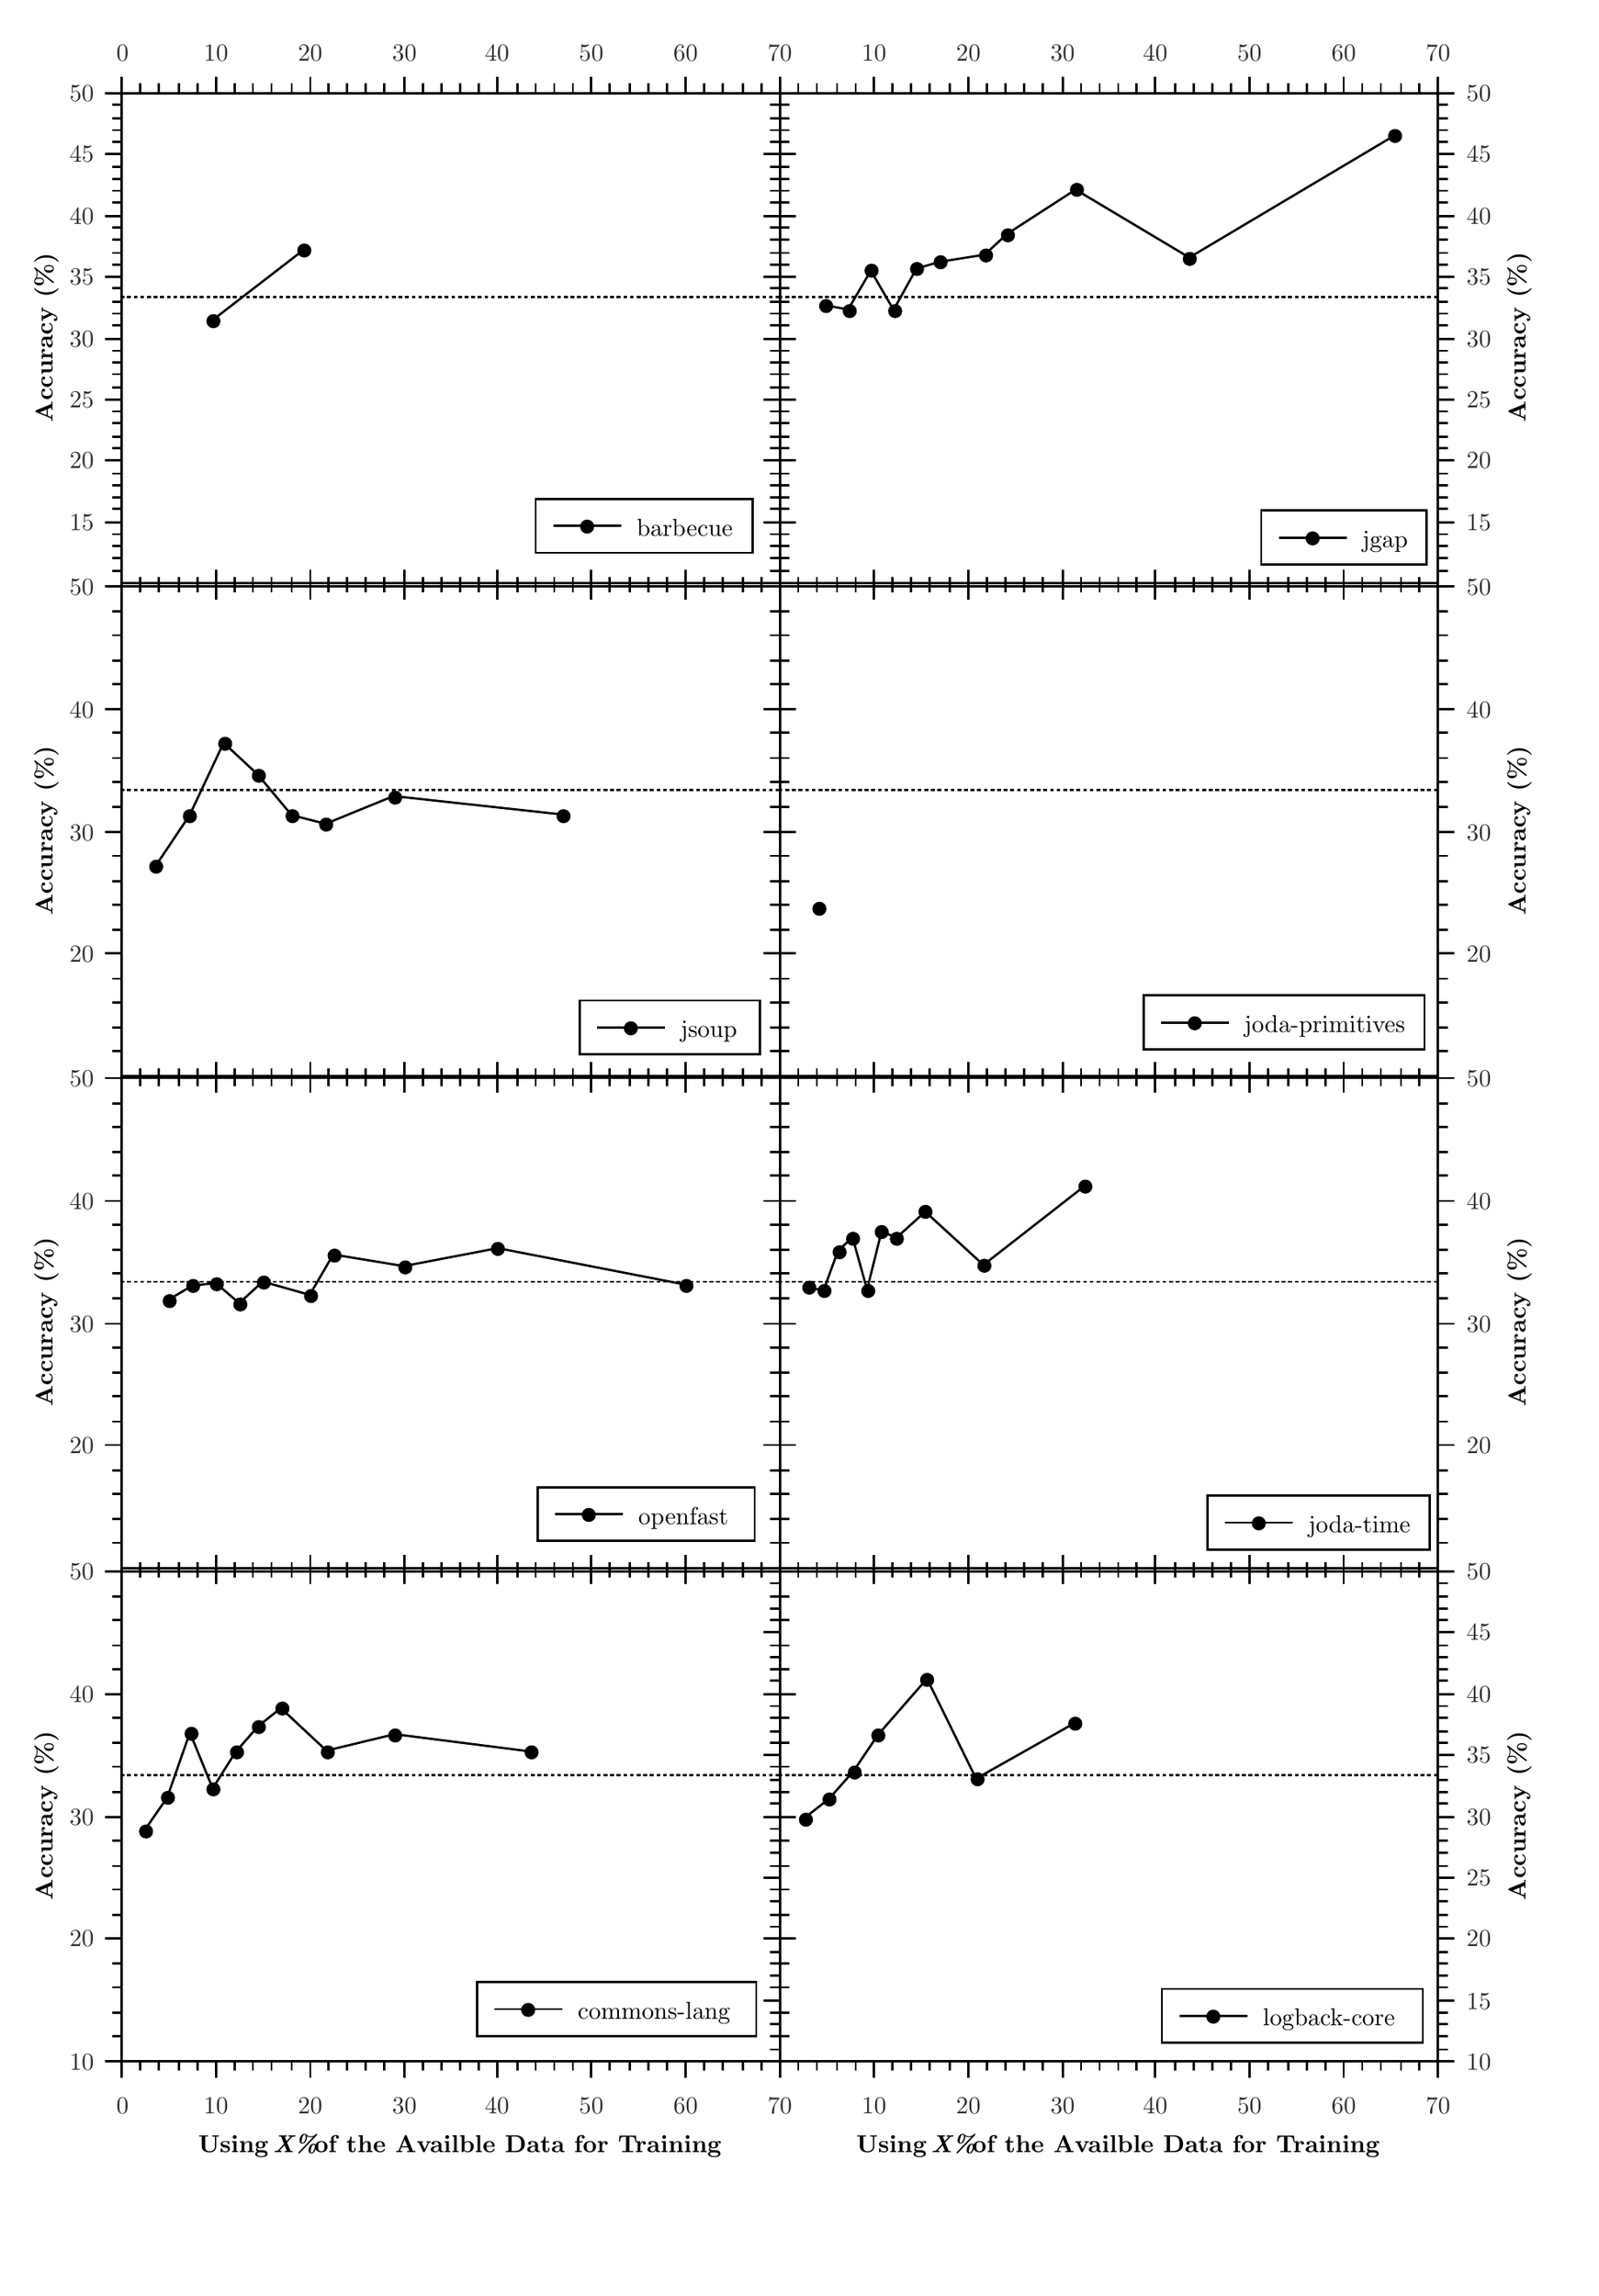
\begin{tikzpicture}{0pt}{0pt}{923pt}{1337pt}
	\clip(0pt,1337pt) -- (694.846pt,1337pt) -- (694.846pt,330.49pt) -- (0pt,330.49pt) -- (0pt,1337pt);
\begin{scope}
	\clip(44.4159pt,864.987pt) -- (338.766pt,864.987pt) -- (338.766pt,645.918pt) -- (44.4159pt,645.918pt) -- (44.4159pt,864.987pt);
	\color[rgb]{0,0,0}
	\draw[line width=1pt, line join=miter, line cap=rect](296.716pt,772.567pt) -- (212.616pt,788.921pt) -- (170.566pt,780.88pt) -- (139.028pt,786.075pt) -- (128.516pt,768.003pt) -- (107.491pt,773.977pt) -- (96.9784pt,764.319pt) -- (86.4659pt,773.37pt) -- (75.9534pt,772.104pt) -- (65.4409pt,765.901pt);
	\color[rgb]{0,0,0}
	\fill(296.985pt,772.014pt) ellipse (2.63484pt and 2.63484pt);
	\draw[line width=1pt, line join=miter, line cap=rect](296.985pt,772.014pt) ellipse (2.63484pt and 2.63484pt);
	\fill(212.67pt,788.576pt) ellipse (2.63484pt and 2.63484pt);
	\draw[line width=1pt, line join=miter, line cap=rect](212.67pt,788.576pt) ellipse (2.63484pt and 2.63484pt);
	\fill(171.265pt,780.295pt) ellipse (2.63484pt and 2.63484pt);
	\draw[line width=1pt, line join=miter, line cap=rect](171.265pt,780.295pt) ellipse (2.63484pt and 2.63484pt);
	\fill(139.647pt,785.565pt) ellipse (2.63484pt and 2.63484pt);
	\draw[line width=1pt, line join=miter, line cap=rect](139.647pt,785.565pt) ellipse (2.63484pt and 2.63484pt);
	\fill(129.107pt,767.497pt) ellipse (2.63484pt and 2.63484pt);
	\draw[line width=1pt, line join=miter, line cap=rect](129.107pt,767.497pt) ellipse (2.63484pt and 2.63484pt);
	\fill(108.029pt,773.52pt) ellipse (2.63484pt and 2.63484pt);
	\draw[line width=1pt, line join=miter, line cap=rect](108.029pt,773.52pt) ellipse (2.63484pt and 2.63484pt);
	\fill(97.4892pt,763.733pt) ellipse (2.63484pt and 2.63484pt);
	\draw[line width=1pt, line join=miter, line cap=rect](97.4892pt,763.733pt) ellipse (2.63484pt and 2.63484pt);
	\fill(86.9498pt,772.767pt) ellipse (2.63484pt and 2.63484pt);
	\draw[line width=1pt, line join=miter, line cap=rect](86.9498pt,772.767pt) ellipse (2.63484pt and 2.63484pt);
	\fill(76.4105pt,772.014pt) ellipse (2.63484pt and 2.63484pt);
	\draw[line width=1pt, line join=miter, line cap=rect](76.4105pt,772.014pt) ellipse (2.63484pt and 2.63484pt);
	\fill(65.8711pt,765.239pt) ellipse (2.63484pt and 2.63484pt);
	\draw[line width=1pt, line join=miter, line cap=rect](65.8711pt,765.239pt) ellipse (2.63484pt and 2.63484pt);
	\draw[line width=1pt, dash pattern=on 0.024cm off 0.08cm, dash phase=0pt, line join=miter, line cap=rect](44.4159pt,773.896pt) -- (465.238pt,773.896pt);
\end{scope}
\begin{scope}
	\color[rgb]{0,0,0}
	\pgftext[center, base, at={\pgfpoint{13.5506pt}{755.823pt}},rotate=90]{\fontsize{11}{0}\selectfont{\textbf{Accuracy (\%)}}}
	\color[rgb]{0.172549,0.172549,0.172549}
	\pgftext[center, base, at={\pgfpoint{26.5719pt}{697.109pt}}]{\fontsize{11}{0}\selectfont{20}}
	\pgftext[center, base, at={\pgfpoint{26.5719pt}{751.312pt}}]{\fontsize{11}{0}\selectfont{30}}
	\pgftext[center, base, at={\pgfpoint{26.5719pt}{806.267pt}}]{\fontsize{11}{0}\selectfont{40}}
	\pgftext[center, base, at={\pgfpoint{26.5719pt}{861.223pt}}]{\fontsize{11}{0}\selectfont{50}}
	\color[rgb]{0,0,0}
	\draw[line width=1pt, line join=bevel, line cap=rect](44.4159pt,657.21pt) -- (40.6519pt,657.21pt);
	\draw[line width=1pt, line join=bevel, line cap=rect](44.4159pt,667.75pt) -- (40.6519pt,667.75pt);
	\draw[line width=1pt, line join=bevel, line cap=rect](44.4159pt,679.042pt) -- (40.6519pt,679.042pt);
	\draw[line width=1pt, line join=bevel, line cap=rect](44.4159pt,689.581pt) -- (40.6519pt,689.581pt);
	\draw[line width=1pt, line join=bevel, line cap=rect](44.4159pt,711.413pt) -- (40.6519pt,711.413pt);
	\draw[line width=1pt, line join=bevel, line cap=rect](44.4159pt,722.705pt) -- (40.6519pt,722.705pt);
	\draw[line width=1pt, line join=bevel, line cap=rect](44.4159pt,733.244pt) -- (40.6519pt,733.244pt);
	\draw[line width=1pt, line join=bevel, line cap=rect](44.4159pt,744.537pt) -- (40.6519pt,744.537pt);
	\draw[line width=1pt, line join=bevel, line cap=rect](44.4159pt,766.368pt) -- (40.6519pt,766.368pt);
	\draw[line width=1pt, line join=bevel, line cap=rect](44.4159pt,777.66pt) -- (40.6519pt,777.66pt);
	\draw[line width=1pt, line join=bevel, line cap=rect](44.4159pt,788.2pt) -- (40.6519pt,788.2pt);
	\draw[line width=1pt, line join=bevel, line cap=rect](44.4159pt,799.492pt) -- (40.6519pt,799.492pt);
	\draw[line width=1pt, line join=bevel, line cap=rect](44.4159pt,821.323pt) -- (40.6519pt,821.323pt);
	\draw[line width=1pt, line join=bevel, line cap=rect](44.4159pt,831.863pt) -- (40.6519pt,831.863pt);
	\draw[line width=1pt, line join=bevel, line cap=rect](44.4159pt,843.155pt) -- (40.6519pt,843.155pt);
	\draw[line width=1pt, line join=bevel, line cap=rect](44.4159pt,853.694pt) -- (40.6519pt,853.694pt);
	\draw[line width=1pt, line join=bevel, line cap=rect](44.4159pt,700.873pt) -- (37.6406pt,700.873pt);
	\draw[line width=1pt, line join=bevel, line cap=rect](44.4159pt,755.076pt) -- (37.6406pt,755.076pt);
	\draw[line width=1pt, line join=bevel, line cap=rect](44.4159pt,810.031pt) -- (37.6406pt,810.031pt);
	\draw[line width=1pt, line join=bevel, line cap=rect](44.4159pt,864.987pt) -- (37.6406pt,864.987pt);
	\draw[line width=1pt, line join=bevel, line cap=rect](44.4159pt,864.987pt) -- (44.4159pt,645.918pt);
	\draw[line width=1pt, line join=bevel, line cap=rect](338.766pt,657.21pt) -- (342.53pt,657.21pt);
	\draw[line width=1pt, line join=bevel, line cap=rect](338.766pt,667.75pt) -- (342.53pt,667.75pt);
	\draw[line width=1pt, line join=bevel, line cap=rect](338.766pt,679.042pt) -- (342.53pt,679.042pt);
	\draw[line width=1pt, line join=bevel, line cap=rect](338.766pt,689.581pt) -- (342.53pt,689.581pt);
	\draw[line width=1pt, line join=bevel, line cap=rect](338.766pt,711.413pt) -- (342.53pt,711.413pt);
	\draw[line width=1pt, line join=bevel, line cap=rect](338.766pt,722.705pt) -- (342.53pt,722.705pt);
	\draw[line width=1pt, line join=bevel, line cap=rect](338.766pt,733.244pt) -- (342.53pt,733.244pt);
	\draw[line width=1pt, line join=bevel, line cap=rect](338.766pt,744.537pt) -- (342.53pt,744.537pt);
	\draw[line width=1pt, line join=bevel, line cap=rect](338.766pt,766.368pt) -- (342.53pt,766.368pt);
	\draw[line width=1pt, line join=bevel, line cap=rect](338.766pt,777.66pt) -- (342.53pt,777.66pt);
	\draw[line width=1pt, line join=bevel, line cap=rect](338.766pt,788.2pt) -- (342.53pt,788.2pt);
	\draw[line width=1pt, line join=bevel, line cap=rect](338.766pt,799.492pt) -- (342.53pt,799.492pt);
	\draw[line width=1pt, line join=bevel, line cap=rect](338.766pt,821.323pt) -- (342.53pt,821.323pt);
	\draw[line width=1pt, line join=bevel, line cap=rect](338.766pt,831.863pt) -- (342.53pt,831.863pt);
	\draw[line width=1pt, line join=bevel, line cap=rect](338.766pt,843.155pt) -- (342.53pt,843.155pt);
	\draw[line width=1pt, line join=bevel, line cap=rect](338.766pt,853.694pt) -- (342.53pt,853.694pt);
	\draw[line width=1pt, line join=bevel, line cap=rect](338.766pt,645.918pt) -- (345.541pt,645.918pt);
	\draw[line width=1pt, line join=bevel, line cap=rect](338.766pt,700.873pt) -- (345.541pt,700.873pt);
	\draw[line width=1pt, line join=bevel, line cap=rect](338.766pt,755.076pt) -- (345.541pt,755.076pt);
	\draw[line width=1pt, line join=bevel, line cap=rect](338.766pt,810.031pt) -- (345.541pt,810.031pt);
	\draw[line width=1pt, line join=bevel, line cap=rect](338.766pt,864.987pt) -- (345.541pt,864.987pt);
	\draw[line width=1pt, line join=bevel, line cap=rect](338.766pt,864.987pt) -- (338.766pt,645.918pt);
	\draw[line width=1pt, line join=bevel, line cap=rect](52.6969pt,645.918pt) -- (52.6969pt,642.154pt);
	\draw[line width=1pt, line join=bevel, line cap=rect](60.9778pt,645.918pt) -- (60.9778pt,642.154pt);
	\draw[line width=1pt, line join=bevel, line cap=rect](70.0116pt,645.918pt) -- (70.0116pt,642.154pt);
	\draw[line width=1pt, line join=bevel, line cap=rect](78.2925pt,645.918pt) -- (78.2925pt,642.154pt);
	\draw[line width=1pt, line join=bevel, line cap=rect](94.8544pt,645.918pt) -- (94.8544pt,642.154pt);
	\draw[line width=1pt, line join=bevel, line cap=rect](103.135pt,645.918pt) -- (103.135pt,642.154pt);
	\draw[line width=1pt, line join=bevel, line cap=rect](111.416pt,645.918pt) -- (111.416pt,642.154pt);
	\draw[line width=1pt, line join=bevel, line cap=rect](120.45pt,645.918pt) -- (120.45pt,642.154pt);
	\draw[line width=1pt, line join=bevel, line cap=rect](137.012pt,645.918pt) -- (137.012pt,642.154pt);
	\draw[line width=1pt, line join=bevel, line cap=rect](145.293pt,645.918pt) -- (145.293pt,642.154pt);
	\draw[line width=1pt, line join=bevel, line cap=rect](153.574pt,645.918pt) -- (153.574pt,642.154pt);
	\draw[line width=1pt, line join=bevel, line cap=rect](161.855pt,645.918pt) -- (161.855pt,642.154pt);
	\draw[line width=1pt, line join=bevel, line cap=rect](179.169pt,645.918pt) -- (179.169pt,642.154pt);
	\draw[line width=1pt, line join=bevel, line cap=rect](187.45pt,645.918pt) -- (187.45pt,642.154pt);
	\draw[line width=1pt, line join=bevel, line cap=rect](195.731pt,645.918pt) -- (195.731pt,642.154pt);
	\draw[line width=1pt, line join=bevel, line cap=rect](204.012pt,645.918pt) -- (204.012pt,642.154pt);
	\draw[line width=1pt, line join=bevel, line cap=rect](221.327pt,645.918pt) -- (221.327pt,642.154pt);
	\draw[line width=1pt, line join=bevel, line cap=rect](229.608pt,645.918pt) -- (229.608pt,642.154pt);
	\draw[line width=1pt, line join=bevel, line cap=rect](237.889pt,645.918pt) -- (237.889pt,642.154pt);
	\draw[line width=1pt, line join=bevel, line cap=rect](246.17pt,645.918pt) -- (246.17pt,642.154pt);
	\draw[line width=1pt, line join=bevel, line cap=rect](262.732pt,645.918pt) -- (262.732pt,642.154pt);
	\draw[line width=1pt, line join=bevel, line cap=rect](271.765pt,645.918pt) -- (271.765pt,642.154pt);
	\draw[line width=1pt, line join=bevel, line cap=rect](280.046pt,645.918pt) -- (280.046pt,642.154pt);
	\draw[line width=1pt, line join=bevel, line cap=rect](288.327pt,645.918pt) -- (288.327pt,642.154pt);
	\draw[line width=1pt, line join=bevel, line cap=rect](304.889pt,645.918pt) -- (304.889pt,642.154pt);
	\draw[line width=1pt, line join=bevel, line cap=rect](313.17pt,645.918pt) -- (313.17pt,642.154pt);
	\draw[line width=1pt, line join=bevel, line cap=rect](322.204pt,645.918pt) -- (322.204pt,642.154pt);
	\draw[line width=1pt, line join=bevel, line cap=rect](330.485pt,645.918pt) -- (330.485pt,642.154pt);
	\draw[line width=1pt, line join=bevel, line cap=rect](44.4159pt,645.918pt) -- (44.4159pt,639.143pt);
	\draw[line width=1pt, line join=bevel, line cap=rect](86.5734pt,645.918pt) -- (86.5734pt,639.143pt);
	\draw[line width=1pt, line join=bevel, line cap=rect](128.731pt,645.918pt) -- (128.731pt,639.143pt);
	\draw[line width=1pt, line join=bevel, line cap=rect](170.888pt,645.918pt) -- (170.888pt,639.143pt);
	\draw[line width=1pt, line join=bevel, line cap=rect](212.293pt,645.918pt) -- (212.293pt,639.143pt);
	\draw[line width=1pt, line join=bevel, line cap=rect](254.451pt,645.918pt) -- (254.451pt,639.143pt);
	\draw[line width=1pt, line join=bevel, line cap=rect](296.608pt,645.918pt) -- (296.608pt,639.143pt);
	\draw[line width=1pt, line join=bevel, line cap=rect](338.766pt,645.918pt) -- (338.766pt,639.143pt);
	\draw[line width=1pt, line join=bevel, line cap=rect](44.4159pt,645.918pt) -- (338.766pt,645.918pt);
	\draw[line width=1pt, line join=bevel, line cap=rect](52.6969pt,864.987pt) -- (52.6969pt,868.751pt);
	\draw[line width=1pt, line join=bevel, line cap=rect](60.9778pt,864.987pt) -- (60.9778pt,868.751pt);
	\draw[line width=1pt, line join=bevel, line cap=rect](70.0116pt,864.987pt) -- (70.0116pt,868.751pt);
	\draw[line width=1pt, line join=bevel, line cap=rect](78.2925pt,864.987pt) -- (78.2925pt,868.751pt);
	\draw[line width=1pt, line join=bevel, line cap=rect](94.8544pt,864.987pt) -- (94.8544pt,868.751pt);
	\draw[line width=1pt, line join=bevel, line cap=rect](103.135pt,864.987pt) -- (103.135pt,868.751pt);
	\draw[line width=1pt, line join=bevel, line cap=rect](111.416pt,864.987pt) -- (111.416pt,868.751pt);
	\draw[line width=1pt, line join=bevel, line cap=rect](120.45pt,864.987pt) -- (120.45pt,868.751pt);
	\draw[line width=1pt, line join=bevel, line cap=rect](137.012pt,864.987pt) -- (137.012pt,868.751pt);
	\draw[line width=1pt, line join=bevel, line cap=rect](145.293pt,864.987pt) -- (145.293pt,868.751pt);
	\draw[line width=1pt, line join=bevel, line cap=rect](153.574pt,864.987pt) -- (153.574pt,868.751pt);
	\draw[line width=1pt, line join=bevel, line cap=rect](161.855pt,864.987pt) -- (161.855pt,868.751pt);
	\draw[line width=1pt, line join=bevel, line cap=rect](179.169pt,864.987pt) -- (179.169pt,868.751pt);
	\draw[line width=1pt, line join=bevel, line cap=rect](187.45pt,864.987pt) -- (187.45pt,868.751pt);
	\draw[line width=1pt, line join=bevel, line cap=rect](195.731pt,864.987pt) -- (195.731pt,868.751pt);
	\draw[line width=1pt, line join=bevel, line cap=rect](204.012pt,864.987pt) -- (204.012pt,868.751pt);
	\draw[line width=1pt, line join=bevel, line cap=rect](221.327pt,864.987pt) -- (221.327pt,868.751pt);
	\draw[line width=1pt, line join=bevel, line cap=rect](229.608pt,864.987pt) -- (229.608pt,868.751pt);
	\draw[line width=1pt, line join=bevel, line cap=rect](237.889pt,864.987pt) -- (237.889pt,868.751pt);
	\draw[line width=1pt, line join=bevel, line cap=rect](246.17pt,864.987pt) -- (246.17pt,868.751pt);
	\draw[line width=1pt, line join=bevel, line cap=rect](262.732pt,864.987pt) -- (262.732pt,868.751pt);
	\draw[line width=1pt, line join=bevel, line cap=rect](271.765pt,864.987pt) -- (271.765pt,868.751pt);
	\draw[line width=1pt, line join=bevel, line cap=rect](280.046pt,864.987pt) -- (280.046pt,868.751pt);
	\draw[line width=1pt, line join=bevel, line cap=rect](288.327pt,864.987pt) -- (288.327pt,868.751pt);
	\draw[line width=1pt, line join=bevel, line cap=rect](304.889pt,864.987pt) -- (304.889pt,868.751pt);
	\draw[line width=1pt, line join=bevel, line cap=rect](313.17pt,864.987pt) -- (313.17pt,868.751pt);
	\draw[line width=1pt, line join=bevel, line cap=rect](322.204pt,864.987pt) -- (322.204pt,868.751pt);
	\draw[line width=1pt, line join=bevel, line cap=rect](330.485pt,864.987pt) -- (330.485pt,868.751pt);
	\draw[line width=1pt, line join=bevel, line cap=rect](44.4159pt,864.987pt) -- (44.4159pt,871.762pt);
	\draw[line width=1pt, line join=bevel, line cap=rect](86.5734pt,864.987pt) -- (86.5734pt,871.762pt);
	\draw[line width=1pt, line join=bevel, line cap=rect](128.731pt,864.987pt) -- (128.731pt,871.762pt);
	\draw[line width=1pt, line join=bevel, line cap=rect](170.888pt,864.987pt) -- (170.888pt,871.762pt);
	\draw[line width=1pt, line join=bevel, line cap=rect](212.293pt,864.987pt) -- (212.293pt,871.762pt);
	\draw[line width=1pt, line join=bevel, line cap=rect](254.451pt,864.987pt) -- (254.451pt,871.762pt);
	\draw[line width=1pt, line join=bevel, line cap=rect](296.608pt,864.987pt) -- (296.608pt,871.762pt);
	\draw[line width=1pt, line join=bevel, line cap=rect](338.766pt,864.987pt) -- (338.766pt,871.762pt);
	\draw[line width=1pt, line join=bevel, line cap=rect](44.4159pt,864.987pt) -- (338.766pt,864.987pt);
	\draw[line width=1pt, line join=miter, line cap=rect](230.361pt,682.053pt) -- (327.473pt,682.053pt) -- (327.473pt,657.963pt) -- (230.361pt,657.963pt) -- (230.361pt,682.053pt);
	\draw[line width=1pt, line join=miter, line cap=rect](238.642pt,670.008pt) -- (268.001pt,670.008pt);
	\fill(253.321pt,669.632pt) ellipse (2.63484pt and 2.63484pt);
	\draw[line width=1pt, line join=miter, line cap=rect](253.321pt,669.632pt) ellipse (2.63484pt and 2.63484pt);
	\pgftext[left, base, at={\pgfpoint{275.529pt}{665.491pt}}]{\fontsize{11}{0}\selectfont{openfast}}
\end{scope}
\begin{scope}
	\clip(338.766pt,864.987pt) -- (633.115pt,864.987pt) -- (633.115pt,645.918pt) -- (338.766pt,645.918pt) -- (338.766pt,864.987pt);
	\color[rgb]{0,0,0}
	\draw[line width=1pt, line join=miter, line cap=rect](475.32pt,816.909pt) -- (429.802pt,781.395pt) -- (403.791pt,805.21pt) -- (390.786pt,793.467pt) -- (384.284pt,796.607pt) -- (377.781pt,770.389pt) -- (371.278pt,793.697pt) -- (364.776pt,787.801pt) -- (358.273pt,769.958pt) -- (351.771pt,771.378pt);
	\color[rgb]{0,0,0}
	\fill(475.401pt,816.43pt) ellipse (2.63484pt and 2.63484pt);
	\draw[line width=1pt, line join=miter, line cap=rect](475.401pt,816.43pt) ellipse (2.63484pt and 2.63484pt);
	\fill(430.232pt,781.048pt) ellipse (2.63484pt and 2.63484pt);
	\draw[line width=1pt, line join=miter, line cap=rect](430.232pt,781.048pt) ellipse (2.63484pt and 2.63484pt);
	\fill(403.884pt,805.138pt) ellipse (2.63484pt and 2.63484pt);
	\draw[line width=1pt, line join=miter, line cap=rect](403.884pt,805.138pt) ellipse (2.63484pt and 2.63484pt);
	\fill(391.086pt,793.093pt) ellipse (2.63484pt and 2.63484pt);
	\draw[line width=1pt, line join=miter, line cap=rect](391.086pt,793.093pt) ellipse (2.63484pt and 2.63484pt);
	\fill(384.311pt,796.104pt) ellipse (2.63484pt and 2.63484pt);
	\draw[line width=1pt, line join=miter, line cap=rect](384.311pt,796.104pt) ellipse (2.63484pt and 2.63484pt);
	\fill(378.288pt,769.756pt) ellipse (2.63484pt and 2.63484pt);
	\draw[line width=1pt, line join=miter, line cap=rect](378.288pt,769.756pt) ellipse (2.63484pt and 2.63484pt);
	\fill(371.513pt,793.093pt) ellipse (2.63484pt and 2.63484pt);
	\draw[line width=1pt, line join=miter, line cap=rect](371.513pt,793.093pt) ellipse (2.63484pt and 2.63484pt);
	\fill(365.49pt,787.07pt) ellipse (2.63484pt and 2.63484pt);
	\draw[line width=1pt, line join=miter, line cap=rect](365.49pt,787.07pt) ellipse (2.63484pt and 2.63484pt);
	\fill(358.715pt,769.756pt) ellipse (2.63484pt and 2.63484pt);
	\draw[line width=1pt, line join=miter, line cap=rect](358.715pt,769.756pt) ellipse (2.63484pt and 2.63484pt);
	\fill(351.94pt,771.261pt) ellipse (2.63484pt and 2.63484pt);
	\draw[line width=1pt, line join=miter, line cap=rect](351.94pt,771.261pt) ellipse (2.63484pt and 2.63484pt);
	\draw[line width=1pt, dash pattern=on 0.024cm off 0.08cm, dash phase=0pt, line join=miter, line cap=rect](338.766pt,773.896pt) -- (759.588pt,773.896pt);
\end{scope}
\begin{scope}
	\color[rgb]{0,0,0}
	\draw[line width=1pt, line join=bevel, line cap=rect](338.766pt,657.21pt) -- (335.002pt,657.21pt);
	\color[rgb]{0,0,0}
	\draw[line width=1pt, line join=bevel, line cap=rect](338.766pt,667.75pt) -- (335.002pt,667.75pt);
	\draw[line width=1pt, line join=bevel, line cap=rect](338.766pt,679.042pt) -- (335.002pt,679.042pt);
	\draw[line width=1pt, line join=bevel, line cap=rect](338.766pt,689.581pt) -- (335.002pt,689.581pt);
	\draw[line width=1pt, line join=bevel, line cap=rect](338.766pt,711.413pt) -- (335.002pt,711.413pt);
	\draw[line width=1pt, line join=bevel, line cap=rect](338.766pt,722.705pt) -- (335.002pt,722.705pt);
	\draw[line width=1pt, line join=bevel, line cap=rect](338.766pt,733.244pt) -- (335.002pt,733.244pt);
	\draw[line width=1pt, line join=bevel, line cap=rect](338.766pt,744.537pt) -- (335.002pt,744.537pt);
	\draw[line width=1pt, line join=bevel, line cap=rect](338.766pt,766.368pt) -- (335.002pt,766.368pt);
	\draw[line width=1pt, line join=bevel, line cap=rect](338.766pt,777.66pt) -- (335.002pt,777.66pt);
	\draw[line width=1pt, line join=bevel, line cap=rect](338.766pt,788.2pt) -- (335.002pt,788.2pt);
	\draw[line width=1pt, line join=bevel, line cap=rect](338.766pt,799.492pt) -- (335.002pt,799.492pt);
	\draw[line width=1pt, line join=bevel, line cap=rect](338.766pt,821.323pt) -- (335.002pt,821.323pt);
	\draw[line width=1pt, line join=bevel, line cap=rect](338.766pt,831.863pt) -- (335.002pt,831.863pt);
	\draw[line width=1pt, line join=bevel, line cap=rect](338.766pt,843.155pt) -- (335.002pt,843.155pt);
	\draw[line width=1pt, line join=bevel, line cap=rect](338.766pt,853.694pt) -- (335.002pt,853.694pt);
	\draw[line width=1pt, line join=bevel, line cap=rect](338.766pt,645.918pt) -- (331.99pt,645.918pt);
	\draw[line width=1pt, line join=bevel, line cap=rect](338.766pt,700.873pt) -- (331.99pt,700.873pt);
	\draw[line width=1pt, line join=bevel, line cap=rect](338.766pt,755.076pt) -- (331.99pt,755.076pt);
	\draw[line width=1pt, line join=bevel, line cap=rect](338.766pt,810.031pt) -- (331.99pt,810.031pt);
	\draw[line width=1pt, line join=bevel, line cap=rect](338.766pt,864.987pt) -- (331.99pt,864.987pt);
	\draw[line width=1pt, line join=bevel, line cap=rect](338.766pt,864.987pt) -- (338.766pt,645.918pt);
	\pgftext[center, base, at={\pgfpoint{672.262pt}{755.823pt}},rotate=90]{\fontsize{11}{0}\selectfont{\textbf{Accuracy (\%)}}}
	\color[rgb]{0.172549,0.172549,0.172549}
	\pgftext[center, base, at={\pgfpoint{651.406pt}{697.109pt}}]{\fontsize{11}{0}\selectfont{20}}
	\pgftext[center, base, at={\pgfpoint{651.406pt}{751.312pt}}]{\fontsize{11}{0}\selectfont{30}}
	\pgftext[center, base, at={\pgfpoint{651.406pt}{806.267pt}}]{\fontsize{11}{0}\selectfont{40}}
	\pgftext[center, base, at={\pgfpoint{651.406pt}{861.223pt}}]{\fontsize{11}{0}\selectfont{50}}
	\color[rgb]{0,0,0}
	\draw[line width=1pt, line join=bevel, line cap=rect](633.115pt,657.21pt) -- (636.879pt,657.21pt);
	\draw[line width=1pt, line join=bevel, line cap=rect](633.115pt,667.75pt) -- (636.879pt,667.75pt);
	\draw[line width=1pt, line join=bevel, line cap=rect](633.115pt,679.042pt) -- (636.879pt,679.042pt);
	\draw[line width=1pt, line join=bevel, line cap=rect](633.115pt,689.581pt) -- (636.879pt,689.581pt);
	\draw[line width=1pt, line join=bevel, line cap=rect](633.115pt,711.413pt) -- (636.879pt,711.413pt);
	\draw[line width=1pt, line join=bevel, line cap=rect](633.115pt,722.705pt) -- (636.879pt,722.705pt);
	\draw[line width=1pt, line join=bevel, line cap=rect](633.115pt,733.244pt) -- (636.879pt,733.244pt);
	\draw[line width=1pt, line join=bevel, line cap=rect](633.115pt,744.537pt) -- (636.879pt,744.537pt);
	\draw[line width=1pt, line join=bevel, line cap=rect](633.115pt,766.368pt) -- (636.879pt,766.368pt);
	\draw[line width=1pt, line join=bevel, line cap=rect](633.115pt,777.66pt) -- (636.879pt,777.66pt);
	\draw[line width=1pt, line join=bevel, line cap=rect](633.115pt,788.2pt) -- (636.879pt,788.2pt);
	\draw[line width=1pt, line join=bevel, line cap=rect](633.115pt,799.492pt) -- (636.879pt,799.492pt);
	\draw[line width=1pt, line join=bevel, line cap=rect](633.115pt,821.323pt) -- (636.879pt,821.323pt);
	\draw[line width=1pt, line join=bevel, line cap=rect](633.115pt,831.863pt) -- (636.879pt,831.863pt);
	\draw[line width=1pt, line join=bevel, line cap=rect](633.115pt,843.155pt) -- (636.879pt,843.155pt);
	\draw[line width=1pt, line join=bevel, line cap=rect](633.115pt,853.694pt) -- (636.879pt,853.694pt);
	\draw[line width=1pt, line join=bevel, line cap=rect](633.115pt,700.873pt) -- (639.891pt,700.873pt);
	\draw[line width=1pt, line join=bevel, line cap=rect](633.115pt,755.076pt) -- (639.891pt,755.076pt);
	\draw[line width=1pt, line join=bevel, line cap=rect](633.115pt,810.031pt) -- (639.891pt,810.031pt);
	\draw[line width=1pt, line join=bevel, line cap=rect](633.115pt,864.987pt) -- (639.891pt,864.987pt);
	\draw[line width=1pt, line join=bevel, line cap=rect](633.115pt,864.987pt) -- (633.115pt,645.918pt);
	\draw[line width=1pt, line join=bevel, line cap=rect](347.047pt,645.918pt) -- (347.047pt,642.154pt);
	\draw[line width=1pt, line join=bevel, line cap=rect](355.327pt,645.918pt) -- (355.327pt,642.154pt);
	\draw[line width=1pt, line join=bevel, line cap=rect](364.361pt,645.918pt) -- (364.361pt,642.154pt);
	\draw[line width=1pt, line join=bevel, line cap=rect](372.642pt,645.918pt) -- (372.642pt,642.154pt);
	\draw[line width=1pt, line join=bevel, line cap=rect](389.204pt,645.918pt) -- (389.204pt,642.154pt);
	\draw[line width=1pt, line join=bevel, line cap=rect](397.485pt,645.918pt) -- (397.485pt,642.154pt);
	\draw[line width=1pt, line join=bevel, line cap=rect](405.766pt,645.918pt) -- (405.766pt,642.154pt);
	\draw[line width=1pt, line join=bevel, line cap=rect](414.8pt,645.918pt) -- (414.8pt,642.154pt);
	\draw[line width=1pt, line join=bevel, line cap=rect](431.362pt,645.918pt) -- (431.362pt,642.154pt);
	\draw[line width=1pt, line join=bevel, line cap=rect](439.642pt,645.918pt) -- (439.642pt,642.154pt);
	\draw[line width=1pt, line join=bevel, line cap=rect](447.923pt,645.918pt) -- (447.923pt,642.154pt);
	\draw[line width=1pt, line join=bevel, line cap=rect](456.204pt,645.918pt) -- (456.204pt,642.154pt);
	\draw[line width=1pt, line join=bevel, line cap=rect](473.519pt,645.918pt) -- (473.519pt,642.154pt);
	\draw[line width=1pt, line join=bevel, line cap=rect](481.8pt,645.918pt) -- (481.8pt,642.154pt);
	\draw[line width=1pt, line join=bevel, line cap=rect](490.081pt,645.918pt) -- (490.081pt,642.154pt);
	\draw[line width=1pt, line join=bevel, line cap=rect](498.362pt,645.918pt) -- (498.362pt,642.154pt);
	\draw[line width=1pt, line join=bevel, line cap=rect](515.677pt,645.918pt) -- (515.677pt,642.154pt);
	\draw[line width=1pt, line join=bevel, line cap=rect](523.957pt,645.918pt) -- (523.957pt,642.154pt);
	\draw[line width=1pt, line join=bevel, line cap=rect](532.238pt,645.918pt) -- (532.238pt,642.154pt);
	\draw[line width=1pt, line join=bevel, line cap=rect](540.519pt,645.918pt) -- (540.519pt,642.154pt);
	\draw[line width=1pt, line join=bevel, line cap=rect](557.081pt,645.918pt) -- (557.081pt,642.154pt);
	\draw[line width=1pt, line join=bevel, line cap=rect](566.115pt,645.918pt) -- (566.115pt,642.154pt);
	\draw[line width=1pt, line join=bevel, line cap=rect](574.396pt,645.918pt) -- (574.396pt,642.154pt);
	\draw[line width=1pt, line join=bevel, line cap=rect](582.677pt,645.918pt) -- (582.677pt,642.154pt);
	\draw[line width=1pt, line join=bevel, line cap=rect](599.239pt,645.918pt) -- (599.239pt,642.154pt);
	\draw[line width=1pt, line join=bevel, line cap=rect](607.52pt,645.918pt) -- (607.52pt,642.154pt);
	\draw[line width=1pt, line join=bevel, line cap=rect](616.553pt,645.918pt) -- (616.553pt,642.154pt);
	\draw[line width=1pt, line join=bevel, line cap=rect](624.834pt,645.918pt) -- (624.834pt,642.154pt);
	\draw[line width=1pt, line join=bevel, line cap=rect](338.766pt,645.918pt) -- (338.766pt,639.143pt);
	\draw[line width=1pt, line join=bevel, line cap=rect](380.923pt,645.918pt) -- (380.923pt,639.143pt);
	\draw[line width=1pt, line join=bevel, line cap=rect](423.081pt,645.918pt) -- (423.081pt,639.143pt);
	\draw[line width=1pt, line join=bevel, line cap=rect](465.238pt,645.918pt) -- (465.238pt,639.143pt);
	\draw[line width=1pt, line join=bevel, line cap=rect](506.643pt,645.918pt) -- (506.643pt,639.143pt);
	\draw[line width=1pt, line join=bevel, line cap=rect](548.8pt,645.918pt) -- (548.8pt,639.143pt);
	\draw[line width=1pt, line join=bevel, line cap=rect](590.958pt,645.918pt) -- (590.958pt,639.143pt);
	\draw[line width=1pt, line join=bevel, line cap=rect](633.115pt,645.918pt) -- (633.115pt,639.143pt);
	\draw[line width=1pt, line join=bevel, line cap=rect](338.766pt,645.918pt) -- (633.115pt,645.918pt);
	\draw[line width=1pt, line join=bevel, line cap=rect](347.047pt,864.987pt) -- (347.047pt,868.751pt);
	\draw[line width=1pt, line join=bevel, line cap=rect](355.327pt,864.987pt) -- (355.327pt,868.751pt);
	\draw[line width=1pt, line join=bevel, line cap=rect](364.361pt,864.987pt) -- (364.361pt,868.751pt);
	\draw[line width=1pt, line join=bevel, line cap=rect](372.642pt,864.987pt) -- (372.642pt,868.751pt);
	\draw[line width=1pt, line join=bevel, line cap=rect](389.204pt,864.987pt) -- (389.204pt,868.751pt);
	\draw[line width=1pt, line join=bevel, line cap=rect](397.485pt,864.987pt) -- (397.485pt,868.751pt);
	\draw[line width=1pt, line join=bevel, line cap=rect](405.766pt,864.987pt) -- (405.766pt,868.751pt);
	\draw[line width=1pt, line join=bevel, line cap=rect](414.8pt,864.987pt) -- (414.8pt,868.751pt);
	\draw[line width=1pt, line join=bevel, line cap=rect](431.362pt,864.987pt) -- (431.362pt,868.751pt);
	\draw[line width=1pt, line join=bevel, line cap=rect](439.642pt,864.987pt) -- (439.642pt,868.751pt);
	\draw[line width=1pt, line join=bevel, line cap=rect](447.923pt,864.987pt) -- (447.923pt,868.751pt);
	\draw[line width=1pt, line join=bevel, line cap=rect](456.204pt,864.987pt) -- (456.204pt,868.751pt);
	\draw[line width=1pt, line join=bevel, line cap=rect](473.519pt,864.987pt) -- (473.519pt,868.751pt);
	\draw[line width=1pt, line join=bevel, line cap=rect](481.8pt,864.987pt) -- (481.8pt,868.751pt);
	\draw[line width=1pt, line join=bevel, line cap=rect](490.081pt,864.987pt) -- (490.081pt,868.751pt);
	\draw[line width=1pt, line join=bevel, line cap=rect](498.362pt,864.987pt) -- (498.362pt,868.751pt);
	\draw[line width=1pt, line join=bevel, line cap=rect](515.677pt,864.987pt) -- (515.677pt,868.751pt);
	\draw[line width=1pt, line join=bevel, line cap=rect](523.957pt,864.987pt) -- (523.957pt,868.751pt);
	\draw[line width=1pt, line join=bevel, line cap=rect](532.238pt,864.987pt) -- (532.238pt,868.751pt);
	\draw[line width=1pt, line join=bevel, line cap=rect](540.519pt,864.987pt) -- (540.519pt,868.751pt);
	\draw[line width=1pt, line join=bevel, line cap=rect](557.081pt,864.987pt) -- (557.081pt,868.751pt);
	\draw[line width=1pt, line join=bevel, line cap=rect](566.115pt,864.987pt) -- (566.115pt,868.751pt);
	\draw[line width=1pt, line join=bevel, line cap=rect](574.396pt,864.987pt) -- (574.396pt,868.751pt);
	\draw[line width=1pt, line join=bevel, line cap=rect](582.677pt,864.987pt) -- (582.677pt,868.751pt);
	\draw[line width=1pt, line join=bevel, line cap=rect](599.239pt,864.987pt) -- (599.239pt,868.751pt);
	\draw[line width=1pt, line join=bevel, line cap=rect](607.52pt,864.987pt) -- (607.52pt,868.751pt);
	\draw[line width=1pt, line join=bevel, line cap=rect](616.553pt,864.987pt) -- (616.553pt,868.751pt);
	\draw[line width=1pt, line join=bevel, line cap=rect](624.834pt,864.987pt) -- (624.834pt,868.751pt);
	\draw[line width=1pt, line join=bevel, line cap=rect](338.766pt,864.987pt) -- (338.766pt,871.762pt);
	\draw[line width=1pt, line join=bevel, line cap=rect](380.923pt,864.987pt) -- (380.923pt,871.762pt);
	\draw[line width=1pt, line join=bevel, line cap=rect](423.081pt,864.987pt) -- (423.081pt,871.762pt);
	\draw[line width=1pt, line join=bevel, line cap=rect](465.238pt,864.987pt) -- (465.238pt,871.762pt);
	\draw[line width=1pt, line join=bevel, line cap=rect](506.643pt,864.987pt) -- (506.643pt,871.762pt);
	\draw[line width=1pt, line join=bevel, line cap=rect](548.8pt,864.987pt) -- (548.8pt,871.762pt);
	\draw[line width=1pt, line join=bevel, line cap=rect](590.958pt,864.987pt) -- (590.958pt,871.762pt);
	\draw[line width=1pt, line join=bevel, line cap=rect](633.115pt,864.987pt) -- (633.115pt,871.762pt);
	\draw[line width=1pt, line join=bevel, line cap=rect](338.766pt,864.987pt) -- (633.115pt,864.987pt);
	\draw[line width=1pt, line join=miter, line cap=rect](529.98pt,678.289pt) -- (629.351pt,678.289pt) -- (629.351pt,654.199pt) -- (529.98pt,654.199pt) -- (529.98pt,678.289pt);
	\draw[line width=1pt, line join=miter, line cap=rect](538.261pt,666.244pt) -- (567.621pt,666.244pt);
	\fill(552.941pt,665.868pt) ellipse (2.63484pt and 2.63484pt);
	\draw[line width=1pt, line join=miter, line cap=rect](552.941pt,665.868pt) ellipse (2.63484pt and 2.63484pt);
	\pgftext[left, base, at={\pgfpoint{575.149pt}{661.727pt}}]{\fontsize{11}{0}\selectfont{joda-time}}
\end{scope}
\begin{scope}
	\clip(338.766pt,644.413pt) -- (633.115pt,644.413pt) -- (633.115pt,425.344pt) -- (338.766pt,425.344pt) -- (338.766pt,644.413pt);
	\color[rgb]{0,0,0}
	\draw[line width=1pt, line join=miter, line cap=rect](470.4pt,576.474pt) -- (426.522pt,551.73pt) -- (404.583pt,596.421pt) -- (382.644pt,571.301pt) -- (371.674pt,555.028pt) -- (360.705pt,542.666pt) -- (349.735pt,534.084pt);
	\color[rgb]{0,0,0}
	\fill(470.884pt,576.283pt) ellipse (2.63484pt and 2.63484pt);
	\draw[line width=1pt, line join=miter, line cap=rect](470.884pt,576.283pt) ellipse (2.63484pt and 2.63484pt);
	\fill(427.221pt,551.44pt) ellipse (2.63484pt and 2.63484pt);
	\draw[line width=1pt, line join=miter, line cap=rect](427.221pt,551.44pt) ellipse (2.63484pt and 2.63484pt);
	\fill(404.637pt,595.856pt) ellipse (2.63484pt and 2.63484pt);
	\draw[line width=1pt, line join=miter, line cap=rect](404.637pt,595.856pt) ellipse (2.63484pt and 2.63484pt);
	\fill(382.805pt,571.013pt) ellipse (2.63484pt and 2.63484pt);
	\draw[line width=1pt, line join=miter, line cap=rect](382.805pt,571.013pt) ellipse (2.63484pt and 2.63484pt);
	\fill(372.266pt,554.451pt) ellipse (2.63484pt and 2.63484pt);
	\draw[line width=1pt, line join=miter, line cap=rect](372.266pt,554.451pt) ellipse (2.63484pt and 2.63484pt);
	\fill(360.974pt,542.406pt) ellipse (2.63484pt and 2.63484pt);
	\draw[line width=1pt, line join=miter, line cap=rect](360.974pt,542.406pt) ellipse (2.63484pt and 2.63484pt);
	\fill(350.434pt,533.373pt) ellipse (2.63484pt and 2.63484pt);
	\draw[line width=1pt, line join=miter, line cap=rect](350.434pt,533.373pt) ellipse (2.63484pt and 2.63484pt);
	\draw[line width=1pt, dash pattern=on 0.024cm off 0.08cm, dash phase=0pt, line join=miter, line cap=rect](338.766pt,553.322pt) -- (759.588pt,553.322pt);
\end{scope}
\begin{scope}
	\color[rgb]{0,0,0}
	\draw[line width=1pt, line join=bevel, line cap=rect](338.766pt,430.614pt) -- (335.002pt,430.614pt);
	\color[rgb]{0,0,0}
	\draw[line width=1pt, line join=bevel, line cap=rect](338.766pt,436.636pt) -- (335.002pt,436.636pt);
	\draw[line width=1pt, line join=bevel, line cap=rect](338.766pt,441.906pt) -- (335.002pt,441.906pt);
	\draw[line width=1pt, line join=bevel, line cap=rect](338.766pt,447.176pt) -- (335.002pt,447.176pt);
	\draw[line width=1pt, line join=bevel, line cap=rect](338.766pt,458.468pt) -- (335.002pt,458.468pt);
	\draw[line width=1pt, line join=bevel, line cap=rect](338.766pt,463.737pt) -- (335.002pt,463.737pt);
	\draw[line width=1pt, line join=bevel, line cap=rect](338.766pt,469.007pt) -- (335.002pt,469.007pt);
	\draw[line width=1pt, line join=bevel, line cap=rect](338.766pt,474.277pt) -- (335.002pt,474.277pt);
	\draw[line width=1pt, line join=bevel, line cap=rect](338.766pt,485.569pt) -- (335.002pt,485.569pt);
	\draw[line width=1pt, line join=bevel, line cap=rect](338.766pt,490.839pt) -- (335.002pt,490.839pt);
	\draw[line width=1pt, line join=bevel, line cap=rect](338.766pt,496.861pt) -- (335.002pt,496.861pt);
	\draw[line width=1pt, line join=bevel, line cap=rect](338.766pt,502.131pt) -- (335.002pt,502.131pt);
	\draw[line width=1pt, line join=bevel, line cap=rect](338.766pt,512.67pt) -- (335.002pt,512.67pt);
	\draw[line width=1pt, line join=bevel, line cap=rect](338.766pt,518.693pt) -- (335.002pt,518.693pt);
	\draw[line width=1pt, line join=bevel, line cap=rect](338.766pt,523.962pt) -- (335.002pt,523.962pt);
	\draw[line width=1pt, line join=bevel, line cap=rect](338.766pt,529.232pt) -- (335.002pt,529.232pt);
	\draw[line width=1pt, line join=bevel, line cap=rect](338.766pt,540.524pt) -- (335.002pt,540.524pt);
	\draw[line width=1pt, line join=bevel, line cap=rect](338.766pt,545.794pt) -- (335.002pt,545.794pt);
	\draw[line width=1pt, line join=bevel, line cap=rect](338.766pt,551.064pt) -- (335.002pt,551.064pt);
	\draw[line width=1pt, line join=bevel, line cap=rect](338.766pt,557.086pt) -- (335.002pt,557.086pt);
	\draw[line width=1pt, line join=bevel, line cap=rect](338.766pt,567.626pt) -- (335.002pt,567.626pt);
	\draw[line width=1pt, line join=bevel, line cap=rect](338.766pt,572.895pt) -- (335.002pt,572.895pt);
	\draw[line width=1pt, line join=bevel, line cap=rect](338.766pt,578.918pt) -- (335.002pt,578.918pt);
	\draw[line width=1pt, line join=bevel, line cap=rect](338.766pt,584.188pt) -- (335.002pt,584.188pt);
	\draw[line width=1pt, line join=bevel, line cap=rect](338.766pt,595.48pt) -- (335.002pt,595.48pt);
	\draw[line width=1pt, line join=bevel, line cap=rect](338.766pt,600.749pt) -- (335.002pt,600.749pt);
	\draw[line width=1pt, line join=bevel, line cap=rect](338.766pt,606.019pt) -- (335.002pt,606.019pt);
	\draw[line width=1pt, line join=bevel, line cap=rect](338.766pt,611.289pt) -- (335.002pt,611.289pt);
	\draw[line width=1pt, line join=bevel, line cap=rect](338.766pt,622.581pt) -- (335.002pt,622.581pt);
	\draw[line width=1pt, line join=bevel, line cap=rect](338.766pt,627.851pt) -- (335.002pt,627.851pt);
	\draw[line width=1pt, line join=bevel, line cap=rect](338.766pt,633.12pt) -- (335.002pt,633.12pt);
	\draw[line width=1pt, line join=bevel, line cap=rect](338.766pt,639.143pt) -- (335.002pt,639.143pt);
	\draw[line width=1pt, line join=bevel, line cap=rect](338.766pt,425.344pt) -- (331.99pt,425.344pt);
	\draw[line width=1pt, line join=bevel, line cap=rect](338.766pt,452.445pt) -- (331.99pt,452.445pt);
	\draw[line width=1pt, line join=bevel, line cap=rect](338.766pt,480.299pt) -- (331.99pt,480.299pt);
	\draw[line width=1pt, line join=bevel, line cap=rect](338.766pt,507.401pt) -- (331.99pt,507.401pt);
	\draw[line width=1pt, line join=bevel, line cap=rect](338.766pt,534.502pt) -- (331.99pt,534.502pt);
	\draw[line width=1pt, line join=bevel, line cap=rect](338.766pt,562.356pt) -- (331.99pt,562.356pt);
	\draw[line width=1pt, line join=bevel, line cap=rect](338.766pt,589.457pt) -- (331.99pt,589.457pt);
	\draw[line width=1pt, line join=bevel, line cap=rect](338.766pt,617.311pt) -- (331.99pt,617.311pt);
	\draw[line width=1pt, line join=bevel, line cap=rect](338.766pt,644.413pt) -- (331.99pt,644.413pt);
	\draw[line width=1pt, line join=bevel, line cap=rect](338.766pt,644.413pt) -- (338.766pt,425.344pt);
	\pgftext[center, base, at={\pgfpoint{672.262pt}{535.249pt}},rotate=90]{\fontsize{11}{0}\selectfont{\textbf{Accuracy (\%)}}}
	\color[rgb]{0.172549,0.172549,0.172549}
	\pgftext[center, base, at={\pgfpoint{651.406pt}{421.58pt}}]{\fontsize{11}{0}\selectfont{10}}
	\pgftext[center, base, at={\pgfpoint{651.406pt}{448.681pt}}]{\fontsize{11}{0}\selectfont{15}}
	\pgftext[center, base, at={\pgfpoint{651.406pt}{476.535pt}}]{\fontsize{11}{0}\selectfont{20}}
	\pgftext[center, base, at={\pgfpoint{651.406pt}{503.637pt}}]{\fontsize{11}{0}\selectfont{25}}
	\pgftext[center, base, at={\pgfpoint{651.406pt}{530.738pt}}]{\fontsize{11}{0}\selectfont{30}}
	\pgftext[center, base, at={\pgfpoint{651.406pt}{558.592pt}}]{\fontsize{11}{0}\selectfont{35}}
	\pgftext[center, base, at={\pgfpoint{651.406pt}{585.693pt}}]{\fontsize{11}{0}\selectfont{40}}
	\pgftext[center, base, at={\pgfpoint{651.406pt}{613.547pt}}]{\fontsize{11}{0}\selectfont{45}}
	\pgftext[center, base, at={\pgfpoint{651.406pt}{640.648pt}}]{\fontsize{11}{0}\selectfont{50}}
	\color[rgb]{0,0,0}
	\draw[line width=1pt, line join=bevel, line cap=rect](633.115pt,430.614pt) -- (636.879pt,430.614pt);
	\draw[line width=1pt, line join=bevel, line cap=rect](633.115pt,436.636pt) -- (636.879pt,436.636pt);
	\draw[line width=1pt, line join=bevel, line cap=rect](633.115pt,441.906pt) -- (636.879pt,441.906pt);
	\draw[line width=1pt, line join=bevel, line cap=rect](633.115pt,447.176pt) -- (636.879pt,447.176pt);
	\draw[line width=1pt, line join=bevel, line cap=rect](633.115pt,458.468pt) -- (636.879pt,458.468pt);
	\draw[line width=1pt, line join=bevel, line cap=rect](633.115pt,463.737pt) -- (636.879pt,463.737pt);
	\draw[line width=1pt, line join=bevel, line cap=rect](633.115pt,469.007pt) -- (636.879pt,469.007pt);
	\draw[line width=1pt, line join=bevel, line cap=rect](633.115pt,474.277pt) -- (636.879pt,474.277pt);
	\draw[line width=1pt, line join=bevel, line cap=rect](633.115pt,485.569pt) -- (636.879pt,485.569pt);
	\draw[line width=1pt, line join=bevel, line cap=rect](633.115pt,490.839pt) -- (636.879pt,490.839pt);
	\draw[line width=1pt, line join=bevel, line cap=rect](633.115pt,496.861pt) -- (636.879pt,496.861pt);
	\draw[line width=1pt, line join=bevel, line cap=rect](633.115pt,502.131pt) -- (636.879pt,502.131pt);
	\draw[line width=1pt, line join=bevel, line cap=rect](633.115pt,512.67pt) -- (636.879pt,512.67pt);
	\draw[line width=1pt, line join=bevel, line cap=rect](633.115pt,518.693pt) -- (636.879pt,518.693pt);
	\draw[line width=1pt, line join=bevel, line cap=rect](633.115pt,523.962pt) -- (636.879pt,523.962pt);
	\draw[line width=1pt, line join=bevel, line cap=rect](633.115pt,529.232pt) -- (636.879pt,529.232pt);
	\draw[line width=1pt, line join=bevel, line cap=rect](633.115pt,540.524pt) -- (636.879pt,540.524pt);
	\draw[line width=1pt, line join=bevel, line cap=rect](633.115pt,545.794pt) -- (636.879pt,545.794pt);
	\draw[line width=1pt, line join=bevel, line cap=rect](633.115pt,551.064pt) -- (636.879pt,551.064pt);
	\draw[line width=1pt, line join=bevel, line cap=rect](633.115pt,557.086pt) -- (636.879pt,557.086pt);
	\draw[line width=1pt, line join=bevel, line cap=rect](633.115pt,567.626pt) -- (636.879pt,567.626pt);
	\draw[line width=1pt, line join=bevel, line cap=rect](633.115pt,572.895pt) -- (636.879pt,572.895pt);
	\draw[line width=1pt, line join=bevel, line cap=rect](633.115pt,578.918pt) -- (636.879pt,578.918pt);
	\draw[line width=1pt, line join=bevel, line cap=rect](633.115pt,584.188pt) -- (636.879pt,584.188pt);
	\draw[line width=1pt, line join=bevel, line cap=rect](633.115pt,595.48pt) -- (636.879pt,595.48pt);
	\draw[line width=1pt, line join=bevel, line cap=rect](633.115pt,600.749pt) -- (636.879pt,600.749pt);
	\draw[line width=1pt, line join=bevel, line cap=rect](633.115pt,606.019pt) -- (636.879pt,606.019pt);
	\draw[line width=1pt, line join=bevel, line cap=rect](633.115pt,611.289pt) -- (636.879pt,611.289pt);
	\draw[line width=1pt, line join=bevel, line cap=rect](633.115pt,622.581pt) -- (636.879pt,622.581pt);
	\draw[line width=1pt, line join=bevel, line cap=rect](633.115pt,627.851pt) -- (636.879pt,627.851pt);
	\draw[line width=1pt, line join=bevel, line cap=rect](633.115pt,633.12pt) -- (636.879pt,633.12pt);
	\draw[line width=1pt, line join=bevel, line cap=rect](633.115pt,639.143pt) -- (636.879pt,639.143pt);
	\draw[line width=1pt, line join=bevel, line cap=rect](633.115pt,425.344pt) -- (639.891pt,425.344pt);
	\draw[line width=1pt, line join=bevel, line cap=rect](633.115pt,452.445pt) -- (639.891pt,452.445pt);
	\draw[line width=1pt, line join=bevel, line cap=rect](633.115pt,480.299pt) -- (639.891pt,480.299pt);
	\draw[line width=1pt, line join=bevel, line cap=rect](633.115pt,507.401pt) -- (639.891pt,507.401pt);
	\draw[line width=1pt, line join=bevel, line cap=rect](633.115pt,534.502pt) -- (639.891pt,534.502pt);
	\draw[line width=1pt, line join=bevel, line cap=rect](633.115pt,562.356pt) -- (639.891pt,562.356pt);
	\draw[line width=1pt, line join=bevel, line cap=rect](633.115pt,589.457pt) -- (639.891pt,589.457pt);
	\draw[line width=1pt, line join=bevel, line cap=rect](633.115pt,617.311pt) -- (639.891pt,617.311pt);
	\draw[line width=1pt, line join=bevel, line cap=rect](633.115pt,644.413pt) -- (639.891pt,644.413pt);
	\draw[line width=1pt, line join=bevel, line cap=rect](633.115pt,644.413pt) -- (633.115pt,425.344pt);
	\pgftext[center, base, at={\pgfpoint{390.927pt}{384.692pt}}]{\fontsize{11}{0}\selectfont{\textbf{Using }}}
	\pgftext[center, base, at={\pgfpoint{417.064pt}{384.692pt}}]{\fontsize{11}{0}\selectfont{\textit{\textbf{X\%}}}}
	\pgftext[center, base, at={\pgfpoint{513.953pt}{384.692pt}}]{\fontsize{11}{0}\selectfont{\textbf{ of the Availble Data for Training}}}
	\color[rgb]{0.172549,0.172549,0.172549}
	\pgftext[center, base, at={\pgfpoint{380.923pt}{402.007pt}}]{\fontsize{11}{0}\selectfont{10}}
	\pgftext[center, base, at={\pgfpoint{423.081pt}{402.007pt}}]{\fontsize{11}{0}\selectfont{20}}
	\pgftext[center, base, at={\pgfpoint{465.238pt}{402.007pt}}]{\fontsize{11}{0}\selectfont{30}}
	\pgftext[center, base, at={\pgfpoint{506.643pt}{402.007pt}}]{\fontsize{11}{0}\selectfont{40}}
	\pgftext[center, base, at={\pgfpoint{548.8pt}{402.007pt}}]{\fontsize{11}{0}\selectfont{50}}
	\pgftext[center, base, at={\pgfpoint{590.958pt}{402.007pt}}]{\fontsize{11}{0}\selectfont{60}}
	\pgftext[center, base, at={\pgfpoint{633.115pt}{402.007pt}}]{\fontsize{11}{0}\selectfont{70}}
	\color[rgb]{0,0,0}
	\draw[line width=1pt, line join=bevel, line cap=rect](347.047pt,425.344pt) -- (347.047pt,421.58pt);
	\draw[line width=1pt, line join=bevel, line cap=rect](355.327pt,425.344pt) -- (355.327pt,421.58pt);
	\draw[line width=1pt, line join=bevel, line cap=rect](364.361pt,425.344pt) -- (364.361pt,421.58pt);
	\draw[line width=1pt, line join=bevel, line cap=rect](372.642pt,425.344pt) -- (372.642pt,421.58pt);
	\draw[line width=1pt, line join=bevel, line cap=rect](389.204pt,425.344pt) -- (389.204pt,421.58pt);
	\draw[line width=1pt, line join=bevel, line cap=rect](397.485pt,425.344pt) -- (397.485pt,421.58pt);
	\draw[line width=1pt, line join=bevel, line cap=rect](405.766pt,425.344pt) -- (405.766pt,421.58pt);
	\draw[line width=1pt, line join=bevel, line cap=rect](414.8pt,425.344pt) -- (414.8pt,421.58pt);
	\draw[line width=1pt, line join=bevel, line cap=rect](431.362pt,425.344pt) -- (431.362pt,421.58pt);
	\draw[line width=1pt, line join=bevel, line cap=rect](439.642pt,425.344pt) -- (439.642pt,421.58pt);
	\draw[line width=1pt, line join=bevel, line cap=rect](447.923pt,425.344pt) -- (447.923pt,421.58pt);
	\draw[line width=1pt, line join=bevel, line cap=rect](456.204pt,425.344pt) -- (456.204pt,421.58pt);
	\draw[line width=1pt, line join=bevel, line cap=rect](473.519pt,425.344pt) -- (473.519pt,421.58pt);
	\draw[line width=1pt, line join=bevel, line cap=rect](481.8pt,425.344pt) -- (481.8pt,421.58pt);
	\draw[line width=1pt, line join=bevel, line cap=rect](490.081pt,425.344pt) -- (490.081pt,421.58pt);
	\draw[line width=1pt, line join=bevel, line cap=rect](498.362pt,425.344pt) -- (498.362pt,421.58pt);
	\draw[line width=1pt, line join=bevel, line cap=rect](515.677pt,425.344pt) -- (515.677pt,421.58pt);
	\draw[line width=1pt, line join=bevel, line cap=rect](523.957pt,425.344pt) -- (523.957pt,421.58pt);
	\draw[line width=1pt, line join=bevel, line cap=rect](532.238pt,425.344pt) -- (532.238pt,421.58pt);
	\draw[line width=1pt, line join=bevel, line cap=rect](540.519pt,425.344pt) -- (540.519pt,421.58pt);
	\draw[line width=1pt, line join=bevel, line cap=rect](557.081pt,425.344pt) -- (557.081pt,421.58pt);
	\draw[line width=1pt, line join=bevel, line cap=rect](566.115pt,425.344pt) -- (566.115pt,421.58pt);
	\draw[line width=1pt, line join=bevel, line cap=rect](574.396pt,425.344pt) -- (574.396pt,421.58pt);
	\draw[line width=1pt, line join=bevel, line cap=rect](582.677pt,425.344pt) -- (582.677pt,421.58pt);
	\draw[line width=1pt, line join=bevel, line cap=rect](599.239pt,425.344pt) -- (599.239pt,421.58pt);
	\draw[line width=1pt, line join=bevel, line cap=rect](607.52pt,425.344pt) -- (607.52pt,421.58pt);
	\draw[line width=1pt, line join=bevel, line cap=rect](616.553pt,425.344pt) -- (616.553pt,421.58pt);
	\draw[line width=1pt, line join=bevel, line cap=rect](624.834pt,425.344pt) -- (624.834pt,421.58pt);
	\draw[line width=1pt, line join=bevel, line cap=rect](380.923pt,425.344pt) -- (380.923pt,418.569pt);
	\draw[line width=1pt, line join=bevel, line cap=rect](423.081pt,425.344pt) -- (423.081pt,418.569pt);
	\draw[line width=1pt, line join=bevel, line cap=rect](465.238pt,425.344pt) -- (465.238pt,418.569pt);
	\draw[line width=1pt, line join=bevel, line cap=rect](506.643pt,425.344pt) -- (506.643pt,418.569pt);
	\draw[line width=1pt, line join=bevel, line cap=rect](548.8pt,425.344pt) -- (548.8pt,418.569pt);
	\draw[line width=1pt, line join=bevel, line cap=rect](590.958pt,425.344pt) -- (590.958pt,418.569pt);
	\draw[line width=1pt, line join=bevel, line cap=rect](633.115pt,425.344pt) -- (633.115pt,418.569pt);
	\draw[line width=1pt, line join=bevel, line cap=rect](338.766pt,425.344pt) -- (633.115pt,425.344pt);
	\draw[line width=1pt, line join=bevel, line cap=rect](347.047pt,644.413pt) -- (347.047pt,648.177pt);
	\draw[line width=1pt, line join=bevel, line cap=rect](355.327pt,644.413pt) -- (355.327pt,648.177pt);
	\draw[line width=1pt, line join=bevel, line cap=rect](364.361pt,644.413pt) -- (364.361pt,648.177pt);
	\draw[line width=1pt, line join=bevel, line cap=rect](372.642pt,644.413pt) -- (372.642pt,648.177pt);
	\draw[line width=1pt, line join=bevel, line cap=rect](389.204pt,644.413pt) -- (389.204pt,648.177pt);
	\draw[line width=1pt, line join=bevel, line cap=rect](397.485pt,644.413pt) -- (397.485pt,648.177pt);
	\draw[line width=1pt, line join=bevel, line cap=rect](405.766pt,644.413pt) -- (405.766pt,648.177pt);
	\draw[line width=1pt, line join=bevel, line cap=rect](414.8pt,644.413pt) -- (414.8pt,648.177pt);
	\draw[line width=1pt, line join=bevel, line cap=rect](431.362pt,644.413pt) -- (431.362pt,648.177pt);
	\draw[line width=1pt, line join=bevel, line cap=rect](439.642pt,644.413pt) -- (439.642pt,648.177pt);
	\draw[line width=1pt, line join=bevel, line cap=rect](447.923pt,644.413pt) -- (447.923pt,648.177pt);
	\draw[line width=1pt, line join=bevel, line cap=rect](456.204pt,644.413pt) -- (456.204pt,648.177pt);
	\draw[line width=1pt, line join=bevel, line cap=rect](473.519pt,644.413pt) -- (473.519pt,648.177pt);
	\draw[line width=1pt, line join=bevel, line cap=rect](481.8pt,644.413pt) -- (481.8pt,648.177pt);
	\draw[line width=1pt, line join=bevel, line cap=rect](490.081pt,644.413pt) -- (490.081pt,648.177pt);
	\draw[line width=1pt, line join=bevel, line cap=rect](498.362pt,644.413pt) -- (498.362pt,648.177pt);
	\draw[line width=1pt, line join=bevel, line cap=rect](515.677pt,644.413pt) -- (515.677pt,648.177pt);
	\draw[line width=1pt, line join=bevel, line cap=rect](523.957pt,644.413pt) -- (523.957pt,648.177pt);
	\draw[line width=1pt, line join=bevel, line cap=rect](532.238pt,644.413pt) -- (532.238pt,648.177pt);
	\draw[line width=1pt, line join=bevel, line cap=rect](540.519pt,644.413pt) -- (540.519pt,648.177pt);
	\draw[line width=1pt, line join=bevel, line cap=rect](557.081pt,644.413pt) -- (557.081pt,648.177pt);
	\draw[line width=1pt, line join=bevel, line cap=rect](566.115pt,644.413pt) -- (566.115pt,648.177pt);
	\draw[line width=1pt, line join=bevel, line cap=rect](574.396pt,644.413pt) -- (574.396pt,648.177pt);
	\draw[line width=1pt, line join=bevel, line cap=rect](582.677pt,644.413pt) -- (582.677pt,648.177pt);
	\draw[line width=1pt, line join=bevel, line cap=rect](599.239pt,644.413pt) -- (599.239pt,648.177pt);
	\draw[line width=1pt, line join=bevel, line cap=rect](607.52pt,644.413pt) -- (607.52pt,648.177pt);
	\draw[line width=1pt, line join=bevel, line cap=rect](616.553pt,644.413pt) -- (616.553pt,648.177pt);
	\draw[line width=1pt, line join=bevel, line cap=rect](624.834pt,644.413pt) -- (624.834pt,648.177pt);
	\draw[line width=1pt, line join=bevel, line cap=rect](338.766pt,644.413pt) -- (338.766pt,651.188pt);
	\draw[line width=1pt, line join=bevel, line cap=rect](380.923pt,644.413pt) -- (380.923pt,651.188pt);
	\draw[line width=1pt, line join=bevel, line cap=rect](423.081pt,644.413pt) -- (423.081pt,651.188pt);
	\draw[line width=1pt, line join=bevel, line cap=rect](465.238pt,644.413pt) -- (465.238pt,651.188pt);
	\draw[line width=1pt, line join=bevel, line cap=rect](506.643pt,644.413pt) -- (506.643pt,651.188pt);
	\draw[line width=1pt, line join=bevel, line cap=rect](548.8pt,644.413pt) -- (548.8pt,651.188pt);
	\draw[line width=1pt, line join=bevel, line cap=rect](590.958pt,644.413pt) -- (590.958pt,651.188pt);
	\draw[line width=1pt, line join=bevel, line cap=rect](633.115pt,644.413pt) -- (633.115pt,651.188pt);
	\draw[line width=1pt, line join=bevel, line cap=rect](338.766pt,644.413pt) -- (633.115pt,644.413pt);
	\draw[line width=1pt, line join=miter, line cap=rect](509.654pt,457.715pt) -- (626.34pt,457.715pt) -- (626.34pt,433.625pt) -- (509.654pt,433.625pt) -- (509.654pt,457.715pt);
	\draw[line width=1pt, line join=miter, line cap=rect](517.935pt,445.67pt) -- (547.295pt,445.67pt);
	\fill(532.615pt,445.294pt) ellipse (2.63484pt and 2.63484pt);
	\draw[line width=1pt, line join=miter, line cap=rect](532.615pt,445.294pt) ellipse (2.63484pt and 2.63484pt);
	\pgftext[left, base, at={\pgfpoint{554.823pt}{441.153pt}}]{\fontsize{11}{0}\selectfont{logback-core}}
\end{scope}
\begin{scope}
	\clip(44.4159pt,644.413pt) -- (338.766pt,644.413pt) -- (338.766pt,425.344pt) -- (44.4159pt,425.344pt) -- (44.4159pt,644.413pt);
	\color[rgb]{0,0,0}
	\draw[line width=1pt, line join=miter, line cap=rect](227.537pt,563.827pt) -- (166.496pt,571.597pt) -- (135.976pt,564.238pt) -- (115.63pt,583.265pt) -- (105.456pt,575.179pt) -- (95.2828pt,563.518pt) -- (85.1094pt,547.348pt) -- (74.9361pt,572.342pt) -- (64.7627pt,543.233pt) -- (54.5893pt,528.542pt);
	\color[rgb]{0,0,0}
	\fill(227.726pt,563.485pt) ellipse (2.63484pt and 2.63484pt);
	\draw[line width=1pt, line join=miter, line cap=rect](227.726pt,563.485pt) ellipse (2.63484pt and 2.63484pt);
	\fill(166.748pt,571.013pt) ellipse (2.63484pt and 2.63484pt);
	\draw[line width=1pt, line join=miter, line cap=rect](166.748pt,571.013pt) ellipse (2.63484pt and 2.63484pt);
	\fill(136.635pt,563.485pt) ellipse (2.63484pt and 2.63484pt);
	\draw[line width=1pt, line join=miter, line cap=rect](136.635pt,563.485pt) ellipse (2.63484pt and 2.63484pt);
	\fill(116.31pt,583.058pt) ellipse (2.63484pt and 2.63484pt);
	\draw[line width=1pt, line join=miter, line cap=rect](116.31pt,583.058pt) ellipse (2.63484pt and 2.63484pt);
	\fill(105.77pt,574.777pt) ellipse (2.63484pt and 2.63484pt);
	\draw[line width=1pt, line join=miter, line cap=rect](105.77pt,574.777pt) ellipse (2.63484pt and 2.63484pt);
	\fill(95.9836pt,563.485pt) ellipse (2.63484pt and 2.63484pt);
	\draw[line width=1pt, line join=miter, line cap=rect](95.9836pt,563.485pt) ellipse (2.63484pt and 2.63484pt);
	\fill(85.4442pt,546.923pt) ellipse (2.63484pt and 2.63484pt);
	\draw[line width=1pt, line join=miter, line cap=rect](85.4442pt,546.923pt) ellipse (2.63484pt and 2.63484pt);
	\fill(75.6577pt,571.766pt) ellipse (2.63484pt and 2.63484pt);
	\draw[line width=1pt, line join=miter, line cap=rect](75.6577pt,571.766pt) ellipse (2.63484pt and 2.63484pt);
	\fill(65.1183pt,543.159pt) ellipse (2.63484pt and 2.63484pt);
	\draw[line width=1pt, line join=miter, line cap=rect](65.1183pt,543.159pt) ellipse (2.63484pt and 2.63484pt);
	\fill(55.3317pt,528.103pt) ellipse (2.63484pt and 2.63484pt);
	\draw[line width=1pt, line join=miter, line cap=rect](55.3317pt,528.103pt) ellipse (2.63484pt and 2.63484pt);
	\draw[line width=1pt, dash pattern=on 0.024cm off 0.08cm, dash phase=0pt, line join=miter, line cap=rect](44.4159pt,553.322pt) -- (465.238pt,553.322pt);
\end{scope}
\begin{scope}
	\color[rgb]{0,0,0}
	\pgftext[center, base, at={\pgfpoint{13.5506pt}{535.249pt}},rotate=90]{\fontsize{11}{0}\selectfont{\textbf{Accuracy (\%)}}}
	\color[rgb]{0.172549,0.172549,0.172549}
	\pgftext[center, base, at={\pgfpoint{26.5719pt}{421.58pt}}]{\fontsize{11}{0}\selectfont{10}}
	\pgftext[center, base, at={\pgfpoint{26.5719pt}{476.535pt}}]{\fontsize{11}{0}\selectfont{20}}
	\pgftext[center, base, at={\pgfpoint{26.5719pt}{530.738pt}}]{\fontsize{11}{0}\selectfont{30}}
	\pgftext[center, base, at={\pgfpoint{26.5719pt}{585.693pt}}]{\fontsize{11}{0}\selectfont{40}}
	\pgftext[center, base, at={\pgfpoint{26.5719pt}{640.648pt}}]{\fontsize{11}{0}\selectfont{50}}
	\color[rgb]{0,0,0}
	\draw[line width=1pt, line join=bevel, line cap=rect](44.4159pt,436.636pt) -- (40.6519pt,436.636pt);
	\draw[line width=1pt, line join=bevel, line cap=rect](44.4159pt,447.176pt) -- (40.6519pt,447.176pt);
	\draw[line width=1pt, line join=bevel, line cap=rect](44.4159pt,458.468pt) -- (40.6519pt,458.468pt);
	\draw[line width=1pt, line join=bevel, line cap=rect](44.4159pt,469.007pt) -- (40.6519pt,469.007pt);
	\draw[line width=1pt, line join=bevel, line cap=rect](44.4159pt,490.839pt) -- (40.6519pt,490.839pt);
	\draw[line width=1pt, line join=bevel, line cap=rect](44.4159pt,502.131pt) -- (40.6519pt,502.131pt);
	\draw[line width=1pt, line join=bevel, line cap=rect](44.4159pt,512.67pt) -- (40.6519pt,512.67pt);
	\draw[line width=1pt, line join=bevel, line cap=rect](44.4159pt,523.962pt) -- (40.6519pt,523.962pt);
	\draw[line width=1pt, line join=bevel, line cap=rect](44.4159pt,545.794pt) -- (40.6519pt,545.794pt);
	\draw[line width=1pt, line join=bevel, line cap=rect](44.4159pt,557.086pt) -- (40.6519pt,557.086pt);
	\draw[line width=1pt, line join=bevel, line cap=rect](44.4159pt,567.626pt) -- (40.6519pt,567.626pt);
	\draw[line width=1pt, line join=bevel, line cap=rect](44.4159pt,578.918pt) -- (40.6519pt,578.918pt);
	\draw[line width=1pt, line join=bevel, line cap=rect](44.4159pt,600.749pt) -- (40.6519pt,600.749pt);
	\draw[line width=1pt, line join=bevel, line cap=rect](44.4159pt,611.289pt) -- (40.6519pt,611.289pt);
	\draw[line width=1pt, line join=bevel, line cap=rect](44.4159pt,622.581pt) -- (40.6519pt,622.581pt);
	\draw[line width=1pt, line join=bevel, line cap=rect](44.4159pt,633.12pt) -- (40.6519pt,633.12pt);
	\draw[line width=1pt, line join=bevel, line cap=rect](44.4159pt,425.344pt) -- (37.6406pt,425.344pt);
	\draw[line width=1pt, line join=bevel, line cap=rect](44.4159pt,480.299pt) -- (37.6406pt,480.299pt);
	\draw[line width=1pt, line join=bevel, line cap=rect](44.4159pt,534.502pt) -- (37.6406pt,534.502pt);
	\draw[line width=1pt, line join=bevel, line cap=rect](44.4159pt,589.457pt) -- (37.6406pt,589.457pt);
	\draw[line width=1pt, line join=bevel, line cap=rect](44.4159pt,644.413pt) -- (37.6406pt,644.413pt);
	\draw[line width=1pt, line join=bevel, line cap=rect](44.4159pt,644.413pt) -- (44.4159pt,425.344pt);
	\draw[line width=1pt, line join=bevel, line cap=rect](338.766pt,436.636pt) -- (342.53pt,436.636pt);
	\draw[line width=1pt, line join=bevel, line cap=rect](338.766pt,447.176pt) -- (342.53pt,447.176pt);
	\draw[line width=1pt, line join=bevel, line cap=rect](338.766pt,458.468pt) -- (342.53pt,458.468pt);
	\draw[line width=1pt, line join=bevel, line cap=rect](338.766pt,469.007pt) -- (342.53pt,469.007pt);
	\draw[line width=1pt, line join=bevel, line cap=rect](338.766pt,490.839pt) -- (342.53pt,490.839pt);
	\draw[line width=1pt, line join=bevel, line cap=rect](338.766pt,502.131pt) -- (342.53pt,502.131pt);
	\draw[line width=1pt, line join=bevel, line cap=rect](338.766pt,512.67pt) -- (342.53pt,512.67pt);
	\draw[line width=1pt, line join=bevel, line cap=rect](338.766pt,523.962pt) -- (342.53pt,523.962pt);
	\draw[line width=1pt, line join=bevel, line cap=rect](338.766pt,545.794pt) -- (342.53pt,545.794pt);
	\draw[line width=1pt, line join=bevel, line cap=rect](338.766pt,557.086pt) -- (342.53pt,557.086pt);
	\draw[line width=1pt, line join=bevel, line cap=rect](338.766pt,567.626pt) -- (342.53pt,567.626pt);
	\draw[line width=1pt, line join=bevel, line cap=rect](338.766pt,578.918pt) -- (342.53pt,578.918pt);
	\draw[line width=1pt, line join=bevel, line cap=rect](338.766pt,600.749pt) -- (342.53pt,600.749pt);
	\draw[line width=1pt, line join=bevel, line cap=rect](338.766pt,611.289pt) -- (342.53pt,611.289pt);
	\draw[line width=1pt, line join=bevel, line cap=rect](338.766pt,622.581pt) -- (342.53pt,622.581pt);
	\draw[line width=1pt, line join=bevel, line cap=rect](338.766pt,633.12pt) -- (342.53pt,633.12pt);
	\draw[line width=1pt, line join=bevel, line cap=rect](338.766pt,425.344pt) -- (345.541pt,425.344pt);
	\draw[line width=1pt, line join=bevel, line cap=rect](338.766pt,480.299pt) -- (345.541pt,480.299pt);
	\draw[line width=1pt, line join=bevel, line cap=rect](338.766pt,534.502pt) -- (345.541pt,534.502pt);
	\draw[line width=1pt, line join=bevel, line cap=rect](338.766pt,589.457pt) -- (345.541pt,589.457pt);
	\draw[line width=1pt, line join=bevel, line cap=rect](338.766pt,644.413pt) -- (345.541pt,644.413pt);
	\draw[line width=1pt, line join=bevel, line cap=rect](338.766pt,644.413pt) -- (338.766pt,425.344pt);
	\pgftext[center, base, at={\pgfpoint{96.5776pt}{384.692pt}}]{\fontsize{11}{0}\selectfont{\textbf{Using }}}
	\pgftext[center, base, at={\pgfpoint{122.714pt}{384.692pt}}]{\fontsize{11}{0}\selectfont{\textit{\textbf{X\%}}}}
	\pgftext[center, base, at={\pgfpoint{219.604pt}{384.692pt}}]{\fontsize{11}{0}\selectfont{\textbf{ of the Availble Data for Training}}}
	\color[rgb]{0.172549,0.172549,0.172549}
	\pgftext[center, base, at={\pgfpoint{44.7865pt}{402.007pt}}]{\fontsize{11}{0}\selectfont{0}}
	\pgftext[center, base, at={\pgfpoint{86.5734pt}{402.007pt}}]{\fontsize{11}{0}\selectfont{10}}
	\pgftext[center, base, at={\pgfpoint{128.731pt}{402.007pt}}]{\fontsize{11}{0}\selectfont{20}}
	\pgftext[center, base, at={\pgfpoint{170.888pt}{402.007pt}}]{\fontsize{11}{0}\selectfont{30}}
	\pgftext[center, base, at={\pgfpoint{212.293pt}{402.007pt}}]{\fontsize{11}{0}\selectfont{40}}
	\pgftext[center, base, at={\pgfpoint{254.451pt}{402.007pt}}]{\fontsize{11}{0}\selectfont{50}}
	\pgftext[center, base, at={\pgfpoint{296.608pt}{402.007pt}}]{\fontsize{11}{0}\selectfont{60}}
	\pgftext[center, base, at={\pgfpoint{338.766pt}{402.007pt}}]{\fontsize{11}{0}\selectfont{70}}
	\color[rgb]{0,0,0}
	\draw[line width=1pt, line join=bevel, line cap=rect](52.6969pt,425.344pt) -- (52.6969pt,421.58pt);
	\draw[line width=1pt, line join=bevel, line cap=rect](60.9778pt,425.344pt) -- (60.9778pt,421.58pt);
	\draw[line width=1pt, line join=bevel, line cap=rect](70.0116pt,425.344pt) -- (70.0116pt,421.58pt);
	\draw[line width=1pt, line join=bevel, line cap=rect](78.2925pt,425.344pt) -- (78.2925pt,421.58pt);
	\draw[line width=1pt, line join=bevel, line cap=rect](94.8544pt,425.344pt) -- (94.8544pt,421.58pt);
	\draw[line width=1pt, line join=bevel, line cap=rect](103.135pt,425.344pt) -- (103.135pt,421.58pt);
	\draw[line width=1pt, line join=bevel, line cap=rect](111.416pt,425.344pt) -- (111.416pt,421.58pt);
	\draw[line width=1pt, line join=bevel, line cap=rect](120.45pt,425.344pt) -- (120.45pt,421.58pt);
	\draw[line width=1pt, line join=bevel, line cap=rect](137.012pt,425.344pt) -- (137.012pt,421.58pt);
	\draw[line width=1pt, line join=bevel, line cap=rect](145.293pt,425.344pt) -- (145.293pt,421.58pt);
	\draw[line width=1pt, line join=bevel, line cap=rect](153.574pt,425.344pt) -- (153.574pt,421.58pt);
	\draw[line width=1pt, line join=bevel, line cap=rect](161.855pt,425.344pt) -- (161.855pt,421.58pt);
	\draw[line width=1pt, line join=bevel, line cap=rect](179.169pt,425.344pt) -- (179.169pt,421.58pt);
	\draw[line width=1pt, line join=bevel, line cap=rect](187.45pt,425.344pt) -- (187.45pt,421.58pt);
	\draw[line width=1pt, line join=bevel, line cap=rect](195.731pt,425.344pt) -- (195.731pt,421.58pt);
	\draw[line width=1pt, line join=bevel, line cap=rect](204.012pt,425.344pt) -- (204.012pt,421.58pt);
	\draw[line width=1pt, line join=bevel, line cap=rect](221.327pt,425.344pt) -- (221.327pt,421.58pt);
	\draw[line width=1pt, line join=bevel, line cap=rect](229.608pt,425.344pt) -- (229.608pt,421.58pt);
	\draw[line width=1pt, line join=bevel, line cap=rect](237.889pt,425.344pt) -- (237.889pt,421.58pt);
	\draw[line width=1pt, line join=bevel, line cap=rect](246.17pt,425.344pt) -- (246.17pt,421.58pt);
	\draw[line width=1pt, line join=bevel, line cap=rect](262.732pt,425.344pt) -- (262.732pt,421.58pt);
	\draw[line width=1pt, line join=bevel, line cap=rect](271.765pt,425.344pt) -- (271.765pt,421.58pt);
	\draw[line width=1pt, line join=bevel, line cap=rect](280.046pt,425.344pt) -- (280.046pt,421.58pt);
	\draw[line width=1pt, line join=bevel, line cap=rect](288.327pt,425.344pt) -- (288.327pt,421.58pt);
	\draw[line width=1pt, line join=bevel, line cap=rect](304.889pt,425.344pt) -- (304.889pt,421.58pt);
	\draw[line width=1pt, line join=bevel, line cap=rect](313.17pt,425.344pt) -- (313.17pt,421.58pt);
	\draw[line width=1pt, line join=bevel, line cap=rect](322.204pt,425.344pt) -- (322.204pt,421.58pt);
	\draw[line width=1pt, line join=bevel, line cap=rect](330.485pt,425.344pt) -- (330.485pt,421.58pt);
	\draw[line width=1pt, line join=bevel, line cap=rect](44.4159pt,425.344pt) -- (44.4159pt,418.569pt);
	\draw[line width=1pt, line join=bevel, line cap=rect](86.5734pt,425.344pt) -- (86.5734pt,418.569pt);
	\draw[line width=1pt, line join=bevel, line cap=rect](128.731pt,425.344pt) -- (128.731pt,418.569pt);
	\draw[line width=1pt, line join=bevel, line cap=rect](170.888pt,425.344pt) -- (170.888pt,418.569pt);
	\draw[line width=1pt, line join=bevel, line cap=rect](212.293pt,425.344pt) -- (212.293pt,418.569pt);
	\draw[line width=1pt, line join=bevel, line cap=rect](254.451pt,425.344pt) -- (254.451pt,418.569pt);
	\draw[line width=1pt, line join=bevel, line cap=rect](296.608pt,425.344pt) -- (296.608pt,418.569pt);
	\draw[line width=1pt, line join=bevel, line cap=rect](338.766pt,425.344pt) -- (338.766pt,418.569pt);
	\draw[line width=1pt, line join=bevel, line cap=rect](44.4159pt,425.344pt) -- (338.766pt,425.344pt);
	\draw[line width=1pt, line join=bevel, line cap=rect](52.6969pt,644.413pt) -- (52.6969pt,648.177pt);
	\draw[line width=1pt, line join=bevel, line cap=rect](60.9778pt,644.413pt) -- (60.9778pt,648.177pt);
	\draw[line width=1pt, line join=bevel, line cap=rect](70.0116pt,644.413pt) -- (70.0116pt,648.177pt);
	\draw[line width=1pt, line join=bevel, line cap=rect](78.2925pt,644.413pt) -- (78.2925pt,648.177pt);
	\draw[line width=1pt, line join=bevel, line cap=rect](94.8544pt,644.413pt) -- (94.8544pt,648.177pt);
	\draw[line width=1pt, line join=bevel, line cap=rect](103.135pt,644.413pt) -- (103.135pt,648.177pt);
	\draw[line width=1pt, line join=bevel, line cap=rect](111.416pt,644.413pt) -- (111.416pt,648.177pt);
	\draw[line width=1pt, line join=bevel, line cap=rect](120.45pt,644.413pt) -- (120.45pt,648.177pt);
	\draw[line width=1pt, line join=bevel, line cap=rect](137.012pt,644.413pt) -- (137.012pt,648.177pt);
	\draw[line width=1pt, line join=bevel, line cap=rect](145.293pt,644.413pt) -- (145.293pt,648.177pt);
	\draw[line width=1pt, line join=bevel, line cap=rect](153.574pt,644.413pt) -- (153.574pt,648.177pt);
	\draw[line width=1pt, line join=bevel, line cap=rect](161.855pt,644.413pt) -- (161.855pt,648.177pt);
	\draw[line width=1pt, line join=bevel, line cap=rect](179.169pt,644.413pt) -- (179.169pt,648.177pt);
	\draw[line width=1pt, line join=bevel, line cap=rect](187.45pt,644.413pt) -- (187.45pt,648.177pt);
	\draw[line width=1pt, line join=bevel, line cap=rect](195.731pt,644.413pt) -- (195.731pt,648.177pt);
	\draw[line width=1pt, line join=bevel, line cap=rect](204.012pt,644.413pt) -- (204.012pt,648.177pt);
	\draw[line width=1pt, line join=bevel, line cap=rect](221.327pt,644.413pt) -- (221.327pt,648.177pt);
	\draw[line width=1pt, line join=bevel, line cap=rect](229.608pt,644.413pt) -- (229.608pt,648.177pt);
	\draw[line width=1pt, line join=bevel, line cap=rect](237.889pt,644.413pt) -- (237.889pt,648.177pt);
	\draw[line width=1pt, line join=bevel, line cap=rect](246.17pt,644.413pt) -- (246.17pt,648.177pt);
	\draw[line width=1pt, line join=bevel, line cap=rect](262.732pt,644.413pt) -- (262.732pt,648.177pt);
	\draw[line width=1pt, line join=bevel, line cap=rect](271.765pt,644.413pt) -- (271.765pt,648.177pt);
	\draw[line width=1pt, line join=bevel, line cap=rect](280.046pt,644.413pt) -- (280.046pt,648.177pt);
	\draw[line width=1pt, line join=bevel, line cap=rect](288.327pt,644.413pt) -- (288.327pt,648.177pt);
	\draw[line width=1pt, line join=bevel, line cap=rect](304.889pt,644.413pt) -- (304.889pt,648.177pt);
	\draw[line width=1pt, line join=bevel, line cap=rect](313.17pt,644.413pt) -- (313.17pt,648.177pt);
	\draw[line width=1pt, line join=bevel, line cap=rect](322.204pt,644.413pt) -- (322.204pt,648.177pt);
	\draw[line width=1pt, line join=bevel, line cap=rect](330.485pt,644.413pt) -- (330.485pt,648.177pt);
	\draw[line width=1pt, line join=bevel, line cap=rect](44.4159pt,644.413pt) -- (44.4159pt,651.188pt);
	\draw[line width=1pt, line join=bevel, line cap=rect](86.5734pt,644.413pt) -- (86.5734pt,651.188pt);
	\draw[line width=1pt, line join=bevel, line cap=rect](128.731pt,644.413pt) -- (128.731pt,651.188pt);
	\draw[line width=1pt, line join=bevel, line cap=rect](170.888pt,644.413pt) -- (170.888pt,651.188pt);
	\draw[line width=1pt, line join=bevel, line cap=rect](212.293pt,644.413pt) -- (212.293pt,651.188pt);
	\draw[line width=1pt, line join=bevel, line cap=rect](254.451pt,644.413pt) -- (254.451pt,651.188pt);
	\draw[line width=1pt, line join=bevel, line cap=rect](296.608pt,644.413pt) -- (296.608pt,651.188pt);
	\draw[line width=1pt, line join=bevel, line cap=rect](338.766pt,644.413pt) -- (338.766pt,651.188pt);
	\draw[line width=1pt, line join=bevel, line cap=rect](44.4159pt,644.413pt) -- (338.766pt,644.413pt);
	\draw[line width=1pt, line join=miter, line cap=rect](203.259pt,460.726pt) -- (328.226pt,460.726pt) -- (328.226pt,436.636pt) -- (203.259pt,436.636pt) -- (203.259pt,460.726pt);
	\draw[line width=1pt, line join=miter, line cap=rect](211.54pt,448.681pt) -- (240.9pt,448.681pt);
	\fill(226.22pt,448.305pt) ellipse (2.63484pt and 2.63484pt);
	\draw[line width=1pt, line join=miter, line cap=rect](226.22pt,448.305pt) ellipse (2.63484pt and 2.63484pt);
	\pgftext[left, base, at={\pgfpoint{248.428pt}{444.164pt}}]{\fontsize{11}{0}\selectfont{commons-lang}}
\end{scope}
\begin{scope}
	\clip(338.766pt,1305.38pt) -- (633.115pt,1305.38pt) -- (633.115pt,1086.31pt) -- (338.766pt,1086.31pt) -- (338.766pt,1305.38pt);
	\color[rgb]{0,0,0}
	\draw[line width=1pt, line join=miter, line cap=rect](613.447pt,1286.28pt) -- (521.886pt,1231.84pt) -- (471.02pt,1262.21pt) -- (440.499pt,1242.46pt) -- (430.326pt,1233.11pt) -- (409.979pt,1229.88pt) -- (399.806pt,1226.85pt) -- (389.633pt,1208.41pt) -- (379.459pt,1226pt) -- (369.286pt,1208.61pt) -- (359.112pt,1210.47pt);
	\color[rgb]{0,0,0}
	\fill(613.919pt,1286.19pt) ellipse (2.63484pt and 2.63484pt);
	\draw[line width=1pt, line join=miter, line cap=rect](613.919pt,1286.19pt) ellipse (2.63484pt and 2.63484pt);
	\fill(522.075pt,1231.23pt) ellipse (2.63484pt and 2.63484pt);
	\draw[line width=1pt, line join=miter, line cap=rect](522.075pt,1231.23pt) ellipse (2.63484pt and 2.63484pt);
	\fill(471.637pt,1262.1pt) ellipse (2.63484pt and 2.63484pt);
	\draw[line width=1pt, line join=miter, line cap=rect](471.637pt,1262.1pt) ellipse (2.63484pt and 2.63484pt);
	\fill(440.772pt,1241.77pt) ellipse (2.63484pt and 2.63484pt);
	\draw[line width=1pt, line join=miter, line cap=rect](440.772pt,1241.77pt) ellipse (2.63484pt and 2.63484pt);
	\fill(430.985pt,1232.74pt) ellipse (2.63484pt and 2.63484pt);
	\draw[line width=1pt, line join=miter, line cap=rect](430.985pt,1232.74pt) ellipse (2.63484pt and 2.63484pt);
	\fill(410.659pt,1229.72pt) ellipse (2.63484pt and 2.63484pt);
	\draw[line width=1pt, line join=miter, line cap=rect](410.659pt,1229.72pt) ellipse (2.63484pt and 2.63484pt);
	\fill(400.12pt,1226.71pt) ellipse (2.63484pt and 2.63484pt);
	\draw[line width=1pt, line join=miter, line cap=rect](400.12pt,1226.71pt) ellipse (2.63484pt and 2.63484pt);
	\fill(390.333pt,1207.89pt) ellipse (2.63484pt and 2.63484pt);
	\draw[line width=1pt, line join=miter, line cap=rect](390.333pt,1207.89pt) ellipse (2.63484pt and 2.63484pt);
	\fill(379.794pt,1225.96pt) ellipse (2.63484pt and 2.63484pt);
	\draw[line width=1pt, line join=miter, line cap=rect](379.794pt,1225.96pt) ellipse (2.63484pt and 2.63484pt);
	\fill(370.007pt,1207.89pt) ellipse (2.63484pt and 2.63484pt);
	\draw[line width=1pt, line join=miter, line cap=rect](370.007pt,1207.89pt) ellipse (2.63484pt and 2.63484pt);
	\fill(359.468pt,1210.15pt) ellipse (2.63484pt and 2.63484pt);
	\draw[line width=1pt, line join=miter, line cap=rect](359.468pt,1210.15pt) ellipse (2.63484pt and 2.63484pt);
	\draw[line width=1pt, dash pattern=on 0.024cm off 0.08cm, dash phase=0pt, line join=miter, line cap=rect](338.766pt,1214.29pt) -- (759.588pt,1214.29pt);
\end{scope}
\begin{scope}
	\color[rgb]{0,0,0}
	\draw[line width=1pt, line join=bevel, line cap=rect](338.766pt,1091.58pt) -- (335.002pt,1091.58pt);
	\color[rgb]{0,0,0}
	\draw[line width=1pt, line join=bevel, line cap=rect](338.766pt,1097.61pt) -- (335.002pt,1097.61pt);
	\draw[line width=1pt, line join=bevel, line cap=rect](338.766pt,1102.88pt) -- (335.002pt,1102.88pt);
	\draw[line width=1pt, line join=bevel, line cap=rect](338.766pt,1108.14pt) -- (335.002pt,1108.14pt);
	\draw[line width=1pt, line join=bevel, line cap=rect](338.766pt,1119.44pt) -- (335.002pt,1119.44pt);
	\draw[line width=1pt, line join=bevel, line cap=rect](338.766pt,1124.71pt) -- (335.002pt,1124.71pt);
	\draw[line width=1pt, line join=bevel, line cap=rect](338.766pt,1129.98pt) -- (335.002pt,1129.98pt);
	\draw[line width=1pt, line join=bevel, line cap=rect](338.766pt,1135.25pt) -- (335.002pt,1135.25pt);
	\draw[line width=1pt, line join=bevel, line cap=rect](338.766pt,1146.54pt) -- (335.002pt,1146.54pt);
	\draw[line width=1pt, line join=bevel, line cap=rect](338.766pt,1151.81pt) -- (335.002pt,1151.81pt);
	\draw[line width=1pt, line join=bevel, line cap=rect](338.766pt,1157.83pt) -- (335.002pt,1157.83pt);
	\draw[line width=1pt, line join=bevel, line cap=rect](338.766pt,1163.1pt) -- (335.002pt,1163.1pt);
	\draw[line width=1pt, line join=bevel, line cap=rect](338.766pt,1173.64pt) -- (335.002pt,1173.64pt);
	\draw[line width=1pt, line join=bevel, line cap=rect](338.766pt,1179.66pt) -- (335.002pt,1179.66pt);
	\draw[line width=1pt, line join=bevel, line cap=rect](338.766pt,1184.93pt) -- (335.002pt,1184.93pt);
	\draw[line width=1pt, line join=bevel, line cap=rect](338.766pt,1190.2pt) -- (335.002pt,1190.2pt);
	\draw[line width=1pt, line join=bevel, line cap=rect](338.766pt,1201.49pt) -- (335.002pt,1201.49pt);
	\draw[line width=1pt, line join=bevel, line cap=rect](338.766pt,1206.76pt) -- (335.002pt,1206.76pt);
	\draw[line width=1pt, line join=bevel, line cap=rect](338.766pt,1212.03pt) -- (335.002pt,1212.03pt);
	\draw[line width=1pt, line join=bevel, line cap=rect](338.766pt,1218.06pt) -- (335.002pt,1218.06pt);
	\draw[line width=1pt, line join=bevel, line cap=rect](338.766pt,1228.6pt) -- (335.002pt,1228.6pt);
	\draw[line width=1pt, line join=bevel, line cap=rect](338.766pt,1233.86pt) -- (335.002pt,1233.86pt);
	\draw[line width=1pt, line join=bevel, line cap=rect](338.766pt,1239.89pt) -- (335.002pt,1239.89pt);
	\draw[line width=1pt, line join=bevel, line cap=rect](338.766pt,1245.16pt) -- (335.002pt,1245.16pt);
	\draw[line width=1pt, line join=bevel, line cap=rect](338.766pt,1256.45pt) -- (335.002pt,1256.45pt);
	\draw[line width=1pt, line join=bevel, line cap=rect](338.766pt,1261.72pt) -- (335.002pt,1261.72pt);
	\draw[line width=1pt, line join=bevel, line cap=rect](338.766pt,1266.99pt) -- (335.002pt,1266.99pt);
	\draw[line width=1pt, line join=bevel, line cap=rect](338.766pt,1272.26pt) -- (335.002pt,1272.26pt);
	\draw[line width=1pt, line join=bevel, line cap=rect](338.766pt,1283.55pt) -- (335.002pt,1283.55pt);
	\draw[line width=1pt, line join=bevel, line cap=rect](338.766pt,1288.82pt) -- (335.002pt,1288.82pt);
	\draw[line width=1pt, line join=bevel, line cap=rect](338.766pt,1294.09pt) -- (335.002pt,1294.09pt);
	\draw[line width=1pt, line join=bevel, line cap=rect](338.766pt,1300.11pt) -- (335.002pt,1300.11pt);
	\draw[line width=1pt, line join=bevel, line cap=rect](338.766pt,1086.31pt) -- (331.99pt,1086.31pt);
	\draw[line width=1pt, line join=bevel, line cap=rect](338.766pt,1113.41pt) -- (331.99pt,1113.41pt);
	\draw[line width=1pt, line join=bevel, line cap=rect](338.766pt,1141.27pt) -- (331.99pt,1141.27pt);
	\draw[line width=1pt, line join=bevel, line cap=rect](338.766pt,1168.37pt) -- (331.99pt,1168.37pt);
	\draw[line width=1pt, line join=bevel, line cap=rect](338.766pt,1195.47pt) -- (331.99pt,1195.47pt);
	\draw[line width=1pt, line join=bevel, line cap=rect](338.766pt,1223.33pt) -- (331.99pt,1223.33pt);
	\draw[line width=1pt, line join=bevel, line cap=rect](338.766pt,1250.43pt) -- (331.99pt,1250.43pt);
	\draw[line width=1pt, line join=bevel, line cap=rect](338.766pt,1278.28pt) -- (331.99pt,1278.28pt);
	\draw[line width=1pt, line join=bevel, line cap=rect](338.766pt,1305.38pt) -- (331.99pt,1305.38pt);
	\draw[line width=1pt, line join=bevel, line cap=rect](338.766pt,1305.38pt) -- (338.766pt,1086.31pt);
	\pgftext[center, base, at={\pgfpoint{672.262pt}{1196.22pt}},rotate=90]{\fontsize{11}{0}\selectfont{\textbf{Accuracy (\%)}}}
	\color[rgb]{0.172549,0.172549,0.172549}
	\pgftext[center, base, at={\pgfpoint{651.406pt}{1109.65pt}}]{\fontsize{11}{0}\selectfont{15}}
	\pgftext[center, base, at={\pgfpoint{651.406pt}{1137.5pt}}]{\fontsize{11}{0}\selectfont{20}}
	\pgftext[center, base, at={\pgfpoint{651.406pt}{1164.61pt}}]{\fontsize{11}{0}\selectfont{25}}
	\pgftext[center, base, at={\pgfpoint{651.406pt}{1191.71pt}}]{\fontsize{11}{0}\selectfont{30}}
	\pgftext[center, base, at={\pgfpoint{651.406pt}{1219.56pt}}]{\fontsize{11}{0}\selectfont{35}}
	\pgftext[center, base, at={\pgfpoint{651.406pt}{1246.66pt}}]{\fontsize{11}{0}\selectfont{40}}
	\pgftext[center, base, at={\pgfpoint{651.406pt}{1274.52pt}}]{\fontsize{11}{0}\selectfont{45}}
	\pgftext[center, base, at={\pgfpoint{651.406pt}{1301.62pt}}]{\fontsize{11}{0}\selectfont{50}}
	\color[rgb]{0,0,0}
	\draw[line width=1pt, line join=bevel, line cap=rect](633.115pt,1091.58pt) -- (636.879pt,1091.58pt);
	\draw[line width=1pt, line join=bevel, line cap=rect](633.115pt,1097.61pt) -- (636.879pt,1097.61pt);
	\draw[line width=1pt, line join=bevel, line cap=rect](633.115pt,1102.88pt) -- (636.879pt,1102.88pt);
	\draw[line width=1pt, line join=bevel, line cap=rect](633.115pt,1108.14pt) -- (636.879pt,1108.14pt);
	\draw[line width=1pt, line join=bevel, line cap=rect](633.115pt,1119.44pt) -- (636.879pt,1119.44pt);
	\draw[line width=1pt, line join=bevel, line cap=rect](633.115pt,1124.71pt) -- (636.879pt,1124.71pt);
	\draw[line width=1pt, line join=bevel, line cap=rect](633.115pt,1129.98pt) -- (636.879pt,1129.98pt);
	\draw[line width=1pt, line join=bevel, line cap=rect](633.115pt,1135.25pt) -- (636.879pt,1135.25pt);
	\draw[line width=1pt, line join=bevel, line cap=rect](633.115pt,1146.54pt) -- (636.879pt,1146.54pt);
	\draw[line width=1pt, line join=bevel, line cap=rect](633.115pt,1151.81pt) -- (636.879pt,1151.81pt);
	\draw[line width=1pt, line join=bevel, line cap=rect](633.115pt,1157.83pt) -- (636.879pt,1157.83pt);
	\draw[line width=1pt, line join=bevel, line cap=rect](633.115pt,1163.1pt) -- (636.879pt,1163.1pt);
	\draw[line width=1pt, line join=bevel, line cap=rect](633.115pt,1173.64pt) -- (636.879pt,1173.64pt);
	\draw[line width=1pt, line join=bevel, line cap=rect](633.115pt,1179.66pt) -- (636.879pt,1179.66pt);
	\draw[line width=1pt, line join=bevel, line cap=rect](633.115pt,1184.93pt) -- (636.879pt,1184.93pt);
	\draw[line width=1pt, line join=bevel, line cap=rect](633.115pt,1190.2pt) -- (636.879pt,1190.2pt);
	\draw[line width=1pt, line join=bevel, line cap=rect](633.115pt,1201.49pt) -- (636.879pt,1201.49pt);
	\draw[line width=1pt, line join=bevel, line cap=rect](633.115pt,1206.76pt) -- (636.879pt,1206.76pt);
	\draw[line width=1pt, line join=bevel, line cap=rect](633.115pt,1212.03pt) -- (636.879pt,1212.03pt);
	\draw[line width=1pt, line join=bevel, line cap=rect](633.115pt,1218.06pt) -- (636.879pt,1218.06pt);
	\draw[line width=1pt, line join=bevel, line cap=rect](633.115pt,1228.6pt) -- (636.879pt,1228.6pt);
	\draw[line width=1pt, line join=bevel, line cap=rect](633.115pt,1233.86pt) -- (636.879pt,1233.86pt);
	\draw[line width=1pt, line join=bevel, line cap=rect](633.115pt,1239.89pt) -- (636.879pt,1239.89pt);
	\draw[line width=1pt, line join=bevel, line cap=rect](633.115pt,1245.16pt) -- (636.879pt,1245.16pt);
	\draw[line width=1pt, line join=bevel, line cap=rect](633.115pt,1256.45pt) -- (636.879pt,1256.45pt);
	\draw[line width=1pt, line join=bevel, line cap=rect](633.115pt,1261.72pt) -- (636.879pt,1261.72pt);
	\draw[line width=1pt, line join=bevel, line cap=rect](633.115pt,1266.99pt) -- (636.879pt,1266.99pt);
	\draw[line width=1pt, line join=bevel, line cap=rect](633.115pt,1272.26pt) -- (636.879pt,1272.26pt);
	\draw[line width=1pt, line join=bevel, line cap=rect](633.115pt,1283.55pt) -- (636.879pt,1283.55pt);
	\draw[line width=1pt, line join=bevel, line cap=rect](633.115pt,1288.82pt) -- (636.879pt,1288.82pt);
	\draw[line width=1pt, line join=bevel, line cap=rect](633.115pt,1294.09pt) -- (636.879pt,1294.09pt);
	\draw[line width=1pt, line join=bevel, line cap=rect](633.115pt,1300.11pt) -- (636.879pt,1300.11pt);
	\draw[line width=1pt, line join=bevel, line cap=rect](633.115pt,1113.41pt) -- (639.891pt,1113.41pt);
	\draw[line width=1pt, line join=bevel, line cap=rect](633.115pt,1141.27pt) -- (639.891pt,1141.27pt);
	\draw[line width=1pt, line join=bevel, line cap=rect](633.115pt,1168.37pt) -- (639.891pt,1168.37pt);
	\draw[line width=1pt, line join=bevel, line cap=rect](633.115pt,1195.47pt) -- (639.891pt,1195.47pt);
	\draw[line width=1pt, line join=bevel, line cap=rect](633.115pt,1223.33pt) -- (639.891pt,1223.33pt);
	\draw[line width=1pt, line join=bevel, line cap=rect](633.115pt,1250.43pt) -- (639.891pt,1250.43pt);
	\draw[line width=1pt, line join=bevel, line cap=rect](633.115pt,1278.28pt) -- (639.891pt,1278.28pt);
	\draw[line width=1pt, line join=bevel, line cap=rect](633.115pt,1305.38pt) -- (639.891pt,1305.38pt);
	\draw[line width=1pt, line join=bevel, line cap=rect](633.115pt,1305.38pt) -- (633.115pt,1086.31pt);
	\draw[line width=1pt, line join=bevel, line cap=rect](347.047pt,1086.31pt) -- (347.047pt,1082.55pt);
	\draw[line width=1pt, line join=bevel, line cap=rect](355.327pt,1086.31pt) -- (355.327pt,1082.55pt);
	\draw[line width=1pt, line join=bevel, line cap=rect](364.361pt,1086.31pt) -- (364.361pt,1082.55pt);
	\draw[line width=1pt, line join=bevel, line cap=rect](372.642pt,1086.31pt) -- (372.642pt,1082.55pt);
	\draw[line width=1pt, line join=bevel, line cap=rect](389.204pt,1086.31pt) -- (389.204pt,1082.55pt);
	\draw[line width=1pt, line join=bevel, line cap=rect](397.485pt,1086.31pt) -- (397.485pt,1082.55pt);
	\draw[line width=1pt, line join=bevel, line cap=rect](405.766pt,1086.31pt) -- (405.766pt,1082.55pt);
	\draw[line width=1pt, line join=bevel, line cap=rect](414.8pt,1086.31pt) -- (414.8pt,1082.55pt);
	\draw[line width=1pt, line join=bevel, line cap=rect](431.362pt,1086.31pt) -- (431.362pt,1082.55pt);
	\draw[line width=1pt, line join=bevel, line cap=rect](439.642pt,1086.31pt) -- (439.642pt,1082.55pt);
	\draw[line width=1pt, line join=bevel, line cap=rect](447.923pt,1086.31pt) -- (447.923pt,1082.55pt);
	\draw[line width=1pt, line join=bevel, line cap=rect](456.204pt,1086.31pt) -- (456.204pt,1082.55pt);
	\draw[line width=1pt, line join=bevel, line cap=rect](473.519pt,1086.31pt) -- (473.519pt,1082.55pt);
	\draw[line width=1pt, line join=bevel, line cap=rect](481.8pt,1086.31pt) -- (481.8pt,1082.55pt);
	\draw[line width=1pt, line join=bevel, line cap=rect](490.081pt,1086.31pt) -- (490.081pt,1082.55pt);
	\draw[line width=1pt, line join=bevel, line cap=rect](498.362pt,1086.31pt) -- (498.362pt,1082.55pt);
	\draw[line width=1pt, line join=bevel, line cap=rect](515.677pt,1086.31pt) -- (515.677pt,1082.55pt);
	\draw[line width=1pt, line join=bevel, line cap=rect](523.957pt,1086.31pt) -- (523.957pt,1082.55pt);
	\draw[line width=1pt, line join=bevel, line cap=rect](532.238pt,1086.31pt) -- (532.238pt,1082.55pt);
	\draw[line width=1pt, line join=bevel, line cap=rect](540.519pt,1086.31pt) -- (540.519pt,1082.55pt);
	\draw[line width=1pt, line join=bevel, line cap=rect](557.081pt,1086.31pt) -- (557.081pt,1082.55pt);
	\draw[line width=1pt, line join=bevel, line cap=rect](566.115pt,1086.31pt) -- (566.115pt,1082.55pt);
	\draw[line width=1pt, line join=bevel, line cap=rect](574.396pt,1086.31pt) -- (574.396pt,1082.55pt);
	\draw[line width=1pt, line join=bevel, line cap=rect](582.677pt,1086.31pt) -- (582.677pt,1082.55pt);
	\draw[line width=1pt, line join=bevel, line cap=rect](599.239pt,1086.31pt) -- (599.239pt,1082.55pt);
	\draw[line width=1pt, line join=bevel, line cap=rect](607.52pt,1086.31pt) -- (607.52pt,1082.55pt);
	\draw[line width=1pt, line join=bevel, line cap=rect](616.553pt,1086.31pt) -- (616.553pt,1082.55pt);
	\draw[line width=1pt, line join=bevel, line cap=rect](624.834pt,1086.31pt) -- (624.834pt,1082.55pt);
	\draw[line width=1pt, line join=bevel, line cap=rect](338.766pt,1086.31pt) -- (338.766pt,1079.54pt);
	\draw[line width=1pt, line join=bevel, line cap=rect](380.923pt,1086.31pt) -- (380.923pt,1079.54pt);
	\draw[line width=1pt, line join=bevel, line cap=rect](423.081pt,1086.31pt) -- (423.081pt,1079.54pt);
	\draw[line width=1pt, line join=bevel, line cap=rect](465.238pt,1086.31pt) -- (465.238pt,1079.54pt);
	\draw[line width=1pt, line join=bevel, line cap=rect](506.643pt,1086.31pt) -- (506.643pt,1079.54pt);
	\draw[line width=1pt, line join=bevel, line cap=rect](548.8pt,1086.31pt) -- (548.8pt,1079.54pt);
	\draw[line width=1pt, line join=bevel, line cap=rect](590.958pt,1086.31pt) -- (590.958pt,1079.54pt);
	\draw[line width=1pt, line join=bevel, line cap=rect](633.115pt,1086.31pt) -- (633.115pt,1079.54pt);
	\draw[line width=1pt, line join=bevel, line cap=rect](338.766pt,1086.31pt) -- (633.115pt,1086.31pt);
	\color[rgb]{0.172549,0.172549,0.172549}
	\pgftext[center, base, at={\pgfpoint{380.923pt}{1319.69pt}}]{\fontsize{11}{0}\selectfont{10}}
	\pgftext[center, base, at={\pgfpoint{423.081pt}{1319.69pt}}]{\fontsize{11}{0}\selectfont{20}}
	\pgftext[center, base, at={\pgfpoint{465.238pt}{1319.69pt}}]{\fontsize{11}{0}\selectfont{30}}
	\pgftext[center, base, at={\pgfpoint{506.643pt}{1319.69pt}}]{\fontsize{11}{0}\selectfont{40}}
	\pgftext[center, base, at={\pgfpoint{548.8pt}{1319.69pt}}]{\fontsize{11}{0}\selectfont{50}}
	\pgftext[center, base, at={\pgfpoint{590.958pt}{1319.69pt}}]{\fontsize{11}{0}\selectfont{60}}
	\pgftext[center, base, at={\pgfpoint{633.115pt}{1319.69pt}}]{\fontsize{11}{0}\selectfont{70}}
	\color[rgb]{0,0,0}
	\draw[line width=1pt, line join=bevel, line cap=rect](347.047pt,1305.38pt) -- (347.047pt,1309.15pt);
	\draw[line width=1pt, line join=bevel, line cap=rect](355.327pt,1305.38pt) -- (355.327pt,1309.15pt);
	\draw[line width=1pt, line join=bevel, line cap=rect](364.361pt,1305.38pt) -- (364.361pt,1309.15pt);
	\draw[line width=1pt, line join=bevel, line cap=rect](372.642pt,1305.38pt) -- (372.642pt,1309.15pt);
	\draw[line width=1pt, line join=bevel, line cap=rect](389.204pt,1305.38pt) -- (389.204pt,1309.15pt);
	\draw[line width=1pt, line join=bevel, line cap=rect](397.485pt,1305.38pt) -- (397.485pt,1309.15pt);
	\draw[line width=1pt, line join=bevel, line cap=rect](405.766pt,1305.38pt) -- (405.766pt,1309.15pt);
	\draw[line width=1pt, line join=bevel, line cap=rect](414.8pt,1305.38pt) -- (414.8pt,1309.15pt);
	\draw[line width=1pt, line join=bevel, line cap=rect](431.362pt,1305.38pt) -- (431.362pt,1309.15pt);
	\draw[line width=1pt, line join=bevel, line cap=rect](439.642pt,1305.38pt) -- (439.642pt,1309.15pt);
	\draw[line width=1pt, line join=bevel, line cap=rect](447.923pt,1305.38pt) -- (447.923pt,1309.15pt);
	\draw[line width=1pt, line join=bevel, line cap=rect](456.204pt,1305.38pt) -- (456.204pt,1309.15pt);
	\draw[line width=1pt, line join=bevel, line cap=rect](473.519pt,1305.38pt) -- (473.519pt,1309.15pt);
	\draw[line width=1pt, line join=bevel, line cap=rect](481.8pt,1305.38pt) -- (481.8pt,1309.15pt);
	\draw[line width=1pt, line join=bevel, line cap=rect](490.081pt,1305.38pt) -- (490.081pt,1309.15pt);
	\draw[line width=1pt, line join=bevel, line cap=rect](498.362pt,1305.38pt) -- (498.362pt,1309.15pt);
	\draw[line width=1pt, line join=bevel, line cap=rect](515.677pt,1305.38pt) -- (515.677pt,1309.15pt);
	\draw[line width=1pt, line join=bevel, line cap=rect](523.957pt,1305.38pt) -- (523.957pt,1309.15pt);
	\draw[line width=1pt, line join=bevel, line cap=rect](532.238pt,1305.38pt) -- (532.238pt,1309.15pt);
	\draw[line width=1pt, line join=bevel, line cap=rect](540.519pt,1305.38pt) -- (540.519pt,1309.15pt);
	\draw[line width=1pt, line join=bevel, line cap=rect](557.081pt,1305.38pt) -- (557.081pt,1309.15pt);
	\draw[line width=1pt, line join=bevel, line cap=rect](566.115pt,1305.38pt) -- (566.115pt,1309.15pt);
	\draw[line width=1pt, line join=bevel, line cap=rect](574.396pt,1305.38pt) -- (574.396pt,1309.15pt);
	\draw[line width=1pt, line join=bevel, line cap=rect](582.677pt,1305.38pt) -- (582.677pt,1309.15pt);
	\draw[line width=1pt, line join=bevel, line cap=rect](599.239pt,1305.38pt) -- (599.239pt,1309.15pt);
	\draw[line width=1pt, line join=bevel, line cap=rect](607.52pt,1305.38pt) -- (607.52pt,1309.15pt);
	\draw[line width=1pt, line join=bevel, line cap=rect](616.553pt,1305.38pt) -- (616.553pt,1309.15pt);
	\draw[line width=1pt, line join=bevel, line cap=rect](624.834pt,1305.38pt) -- (624.834pt,1309.15pt);
	\draw[line width=1pt, line join=bevel, line cap=rect](380.923pt,1305.38pt) -- (380.923pt,1312.16pt);
	\draw[line width=1pt, line join=bevel, line cap=rect](423.081pt,1305.38pt) -- (423.081pt,1312.16pt);
	\draw[line width=1pt, line join=bevel, line cap=rect](465.238pt,1305.38pt) -- (465.238pt,1312.16pt);
	\draw[line width=1pt, line join=bevel, line cap=rect](506.643pt,1305.38pt) -- (506.643pt,1312.16pt);
	\draw[line width=1pt, line join=bevel, line cap=rect](548.8pt,1305.38pt) -- (548.8pt,1312.16pt);
	\draw[line width=1pt, line join=bevel, line cap=rect](590.958pt,1305.38pt) -- (590.958pt,1312.16pt);
	\draw[line width=1pt, line join=bevel, line cap=rect](633.115pt,1305.38pt) -- (633.115pt,1312.16pt);
	\draw[line width=1pt, line join=bevel, line cap=rect](338.766pt,1305.38pt) -- (633.115pt,1305.38pt);
	\draw[line width=1pt, line join=miter, line cap=rect](554.07pt,1118.68pt) -- (627.846pt,1118.68pt) -- (627.846pt,1094.59pt) -- (554.07pt,1094.59pt) -- (554.07pt,1118.68pt);
	\draw[line width=1pt, line join=miter, line cap=rect](562.351pt,1106.64pt) -- (591.711pt,1106.64pt);
	\fill(577.031pt,1106.26pt) ellipse (2.63484pt and 2.63484pt);
	\draw[line width=1pt, line join=miter, line cap=rect](577.031pt,1106.26pt) ellipse (2.63484pt and 2.63484pt);
	\pgftext[left, base, at={\pgfpoint{599.239pt}{1102.12pt}}]{\fontsize{11}{0}\selectfont{jgap}}
\end{scope}
\begin{scope}
	\clip(338.766pt,1084.81pt) -- (633.115pt,1084.81pt) -- (633.115pt,865.739pt) -- (338.766pt,865.739pt) -- (338.766pt,1084.81pt);
	\color[rgb]{0,0,0}
	\fill(356.457pt,940.644pt) ellipse (2.63484pt and 2.63484pt);
	\draw[line width=1pt, line join=miter, line cap=rect](356.457pt,940.644pt) ellipse (2.63484pt and 2.63484pt);
	\color[rgb]{0,0,0}
	\draw[line width=1pt, dash pattern=on 0.024cm off 0.08cm, dash phase=0pt, line join=miter, line cap=rect](338.766pt,993.717pt) -- (759.588pt,993.717pt);
\end{scope}
\begin{scope}
	\color[rgb]{0,0,0}
	\draw[line width=1pt, line join=bevel, line cap=rect](338.766pt,877.032pt) -- (335.002pt,877.032pt);
	\color[rgb]{0,0,0}
	\draw[line width=1pt, line join=bevel, line cap=rect](338.766pt,887.571pt) -- (335.002pt,887.571pt);
	\draw[line width=1pt, line join=bevel, line cap=rect](338.766pt,898.863pt) -- (335.002pt,898.863pt);
	\draw[line width=1pt, line join=bevel, line cap=rect](338.766pt,909.402pt) -- (335.002pt,909.402pt);
	\draw[line width=1pt, line join=bevel, line cap=rect](338.766pt,931.234pt) -- (335.002pt,931.234pt);
	\draw[line width=1pt, line join=bevel, line cap=rect](338.766pt,942.526pt) -- (335.002pt,942.526pt);
	\draw[line width=1pt, line join=bevel, line cap=rect](338.766pt,953.066pt) -- (335.002pt,953.066pt);
	\draw[line width=1pt, line join=bevel, line cap=rect](338.766pt,964.358pt) -- (335.002pt,964.358pt);
	\draw[line width=1pt, line join=bevel, line cap=rect](338.766pt,986.189pt) -- (335.002pt,986.189pt);
	\draw[line width=1pt, line join=bevel, line cap=rect](338.766pt,997.482pt) -- (335.002pt,997.482pt);
	\draw[line width=1pt, line join=bevel, line cap=rect](338.766pt,1008.02pt) -- (335.002pt,1008.02pt);
	\draw[line width=1pt, line join=bevel, line cap=rect](338.766pt,1019.31pt) -- (335.002pt,1019.31pt);
	\draw[line width=1pt, line join=bevel, line cap=rect](338.766pt,1041.14pt) -- (335.002pt,1041.14pt);
	\draw[line width=1pt, line join=bevel, line cap=rect](338.766pt,1051.68pt) -- (335.002pt,1051.68pt);
	\draw[line width=1pt, line join=bevel, line cap=rect](338.766pt,1062.98pt) -- (335.002pt,1062.98pt);
	\draw[line width=1pt, line join=bevel, line cap=rect](338.766pt,1073.52pt) -- (335.002pt,1073.52pt);
	\draw[line width=1pt, line join=bevel, line cap=rect](338.766pt,865.739pt) -- (331.99pt,865.739pt);
	\draw[line width=1pt, line join=bevel, line cap=rect](338.766pt,920.695pt) -- (331.99pt,920.695pt);
	\draw[line width=1pt, line join=bevel, line cap=rect](338.766pt,974.897pt) -- (331.99pt,974.897pt);
	\draw[line width=1pt, line join=bevel, line cap=rect](338.766pt,1029.85pt) -- (331.99pt,1029.85pt);
	\draw[line width=1pt, line join=bevel, line cap=rect](338.766pt,1084.81pt) -- (331.99pt,1084.81pt);
	\draw[line width=1pt, line join=bevel, line cap=rect](338.766pt,1084.81pt) -- (338.766pt,865.739pt);
	\pgftext[center, base, at={\pgfpoint{672.262pt}{975.644pt}},rotate=90]{\fontsize{11}{0}\selectfont{\textbf{Accuracy (\%)}}}
	\color[rgb]{0.172549,0.172549,0.172549}
	\pgftext[center, base, at={\pgfpoint{651.406pt}{916.931pt}}]{\fontsize{11}{0}\selectfont{20}}
	\pgftext[center, base, at={\pgfpoint{651.406pt}{971.133pt}}]{\fontsize{11}{0}\selectfont{30}}
	\pgftext[center, base, at={\pgfpoint{651.406pt}{1026.09pt}}]{\fontsize{11}{0}\selectfont{40}}
	\pgftext[center, base, at={\pgfpoint{651.406pt}{1081.04pt}}]{\fontsize{11}{0}\selectfont{50}}
	\color[rgb]{0,0,0}
	\draw[line width=1pt, line join=bevel, line cap=rect](633.115pt,877.032pt) -- (636.879pt,877.032pt);
	\draw[line width=1pt, line join=bevel, line cap=rect](633.115pt,887.571pt) -- (636.879pt,887.571pt);
	\draw[line width=1pt, line join=bevel, line cap=rect](633.115pt,898.863pt) -- (636.879pt,898.863pt);
	\draw[line width=1pt, line join=bevel, line cap=rect](633.115pt,909.402pt) -- (636.879pt,909.402pt);
	\draw[line width=1pt, line join=bevel, line cap=rect](633.115pt,931.234pt) -- (636.879pt,931.234pt);
	\draw[line width=1pt, line join=bevel, line cap=rect](633.115pt,942.526pt) -- (636.879pt,942.526pt);
	\draw[line width=1pt, line join=bevel, line cap=rect](633.115pt,953.066pt) -- (636.879pt,953.066pt);
	\draw[line width=1pt, line join=bevel, line cap=rect](633.115pt,964.358pt) -- (636.879pt,964.358pt);
	\draw[line width=1pt, line join=bevel, line cap=rect](633.115pt,986.189pt) -- (636.879pt,986.189pt);
	\draw[line width=1pt, line join=bevel, line cap=rect](633.115pt,997.482pt) -- (636.879pt,997.482pt);
	\draw[line width=1pt, line join=bevel, line cap=rect](633.115pt,1008.02pt) -- (636.879pt,1008.02pt);
	\draw[line width=1pt, line join=bevel, line cap=rect](633.115pt,1019.31pt) -- (636.879pt,1019.31pt);
	\draw[line width=1pt, line join=bevel, line cap=rect](633.115pt,1041.14pt) -- (636.879pt,1041.14pt);
	\draw[line width=1pt, line join=bevel, line cap=rect](633.115pt,1051.68pt) -- (636.879pt,1051.68pt);
	\draw[line width=1pt, line join=bevel, line cap=rect](633.115pt,1062.98pt) -- (636.879pt,1062.98pt);
	\draw[line width=1pt, line join=bevel, line cap=rect](633.115pt,1073.52pt) -- (636.879pt,1073.52pt);
	\draw[line width=1pt, line join=bevel, line cap=rect](633.115pt,920.695pt) -- (639.891pt,920.695pt);
	\draw[line width=1pt, line join=bevel, line cap=rect](633.115pt,974.897pt) -- (639.891pt,974.897pt);
	\draw[line width=1pt, line join=bevel, line cap=rect](633.115pt,1029.85pt) -- (639.891pt,1029.85pt);
	\draw[line width=1pt, line join=bevel, line cap=rect](633.115pt,1084.81pt) -- (639.891pt,1084.81pt);
	\draw[line width=1pt, line join=bevel, line cap=rect](633.115pt,1084.81pt) -- (633.115pt,865.739pt);
	\draw[line width=1pt, line join=bevel, line cap=rect](347.047pt,865.739pt) -- (347.047pt,861.975pt);
	\draw[line width=1pt, line join=bevel, line cap=rect](355.327pt,865.739pt) -- (355.327pt,861.975pt);
	\draw[line width=1pt, line join=bevel, line cap=rect](364.361pt,865.739pt) -- (364.361pt,861.975pt);
	\draw[line width=1pt, line join=bevel, line cap=rect](372.642pt,865.739pt) -- (372.642pt,861.975pt);
	\draw[line width=1pt, line join=bevel, line cap=rect](389.204pt,865.739pt) -- (389.204pt,861.975pt);
	\draw[line width=1pt, line join=bevel, line cap=rect](397.485pt,865.739pt) -- (397.485pt,861.975pt);
	\draw[line width=1pt, line join=bevel, line cap=rect](405.766pt,865.739pt) -- (405.766pt,861.975pt);
	\draw[line width=1pt, line join=bevel, line cap=rect](414.8pt,865.739pt) -- (414.8pt,861.975pt);
	\draw[line width=1pt, line join=bevel, line cap=rect](431.362pt,865.739pt) -- (431.362pt,861.975pt);
	\draw[line width=1pt, line join=bevel, line cap=rect](439.642pt,865.739pt) -- (439.642pt,861.975pt);
	\draw[line width=1pt, line join=bevel, line cap=rect](447.923pt,865.739pt) -- (447.923pt,861.975pt);
	\draw[line width=1pt, line join=bevel, line cap=rect](456.204pt,865.739pt) -- (456.204pt,861.975pt);
	\draw[line width=1pt, line join=bevel, line cap=rect](473.519pt,865.739pt) -- (473.519pt,861.975pt);
	\draw[line width=1pt, line join=bevel, line cap=rect](481.8pt,865.739pt) -- (481.8pt,861.975pt);
	\draw[line width=1pt, line join=bevel, line cap=rect](490.081pt,865.739pt) -- (490.081pt,861.975pt);
	\draw[line width=1pt, line join=bevel, line cap=rect](498.362pt,865.739pt) -- (498.362pt,861.975pt);
	\draw[line width=1pt, line join=bevel, line cap=rect](515.677pt,865.739pt) -- (515.677pt,861.975pt);
	\draw[line width=1pt, line join=bevel, line cap=rect](523.957pt,865.739pt) -- (523.957pt,861.975pt);
	\draw[line width=1pt, line join=bevel, line cap=rect](532.238pt,865.739pt) -- (532.238pt,861.975pt);
	\draw[line width=1pt, line join=bevel, line cap=rect](540.519pt,865.739pt) -- (540.519pt,861.975pt);
	\draw[line width=1pt, line join=bevel, line cap=rect](557.081pt,865.739pt) -- (557.081pt,861.975pt);
	\draw[line width=1pt, line join=bevel, line cap=rect](566.115pt,865.739pt) -- (566.115pt,861.975pt);
	\draw[line width=1pt, line join=bevel, line cap=rect](574.396pt,865.739pt) -- (574.396pt,861.975pt);
	\draw[line width=1pt, line join=bevel, line cap=rect](582.677pt,865.739pt) -- (582.677pt,861.975pt);
	\draw[line width=1pt, line join=bevel, line cap=rect](599.239pt,865.739pt) -- (599.239pt,861.975pt);
	\draw[line width=1pt, line join=bevel, line cap=rect](607.52pt,865.739pt) -- (607.52pt,861.975pt);
	\draw[line width=1pt, line join=bevel, line cap=rect](616.553pt,865.739pt) -- (616.553pt,861.975pt);
	\draw[line width=1pt, line join=bevel, line cap=rect](624.834pt,865.739pt) -- (624.834pt,861.975pt);
	\draw[line width=1pt, line join=bevel, line cap=rect](338.766pt,865.739pt) -- (338.766pt,858.964pt);
	\draw[line width=1pt, line join=bevel, line cap=rect](380.923pt,865.739pt) -- (380.923pt,858.964pt);
	\draw[line width=1pt, line join=bevel, line cap=rect](423.081pt,865.739pt) -- (423.081pt,858.964pt);
	\draw[line width=1pt, line join=bevel, line cap=rect](465.238pt,865.739pt) -- (465.238pt,858.964pt);
	\draw[line width=1pt, line join=bevel, line cap=rect](506.643pt,865.739pt) -- (506.643pt,858.964pt);
	\draw[line width=1pt, line join=bevel, line cap=rect](548.8pt,865.739pt) -- (548.8pt,858.964pt);
	\draw[line width=1pt, line join=bevel, line cap=rect](590.958pt,865.739pt) -- (590.958pt,858.964pt);
	\draw[line width=1pt, line join=bevel, line cap=rect](633.115pt,865.739pt) -- (633.115pt,858.964pt);
	\draw[line width=1pt, line join=bevel, line cap=rect](338.766pt,865.739pt) -- (633.115pt,865.739pt);
	\draw[line width=1pt, line join=bevel, line cap=rect](347.047pt,1084.81pt) -- (347.047pt,1088.57pt);
	\draw[line width=1pt, line join=bevel, line cap=rect](355.327pt,1084.81pt) -- (355.327pt,1088.57pt);
	\draw[line width=1pt, line join=bevel, line cap=rect](364.361pt,1084.81pt) -- (364.361pt,1088.57pt);
	\draw[line width=1pt, line join=bevel, line cap=rect](372.642pt,1084.81pt) -- (372.642pt,1088.57pt);
	\draw[line width=1pt, line join=bevel, line cap=rect](389.204pt,1084.81pt) -- (389.204pt,1088.57pt);
	\draw[line width=1pt, line join=bevel, line cap=rect](397.485pt,1084.81pt) -- (397.485pt,1088.57pt);
	\draw[line width=1pt, line join=bevel, line cap=rect](405.766pt,1084.81pt) -- (405.766pt,1088.57pt);
	\draw[line width=1pt, line join=bevel, line cap=rect](414.8pt,1084.81pt) -- (414.8pt,1088.57pt);
	\draw[line width=1pt, line join=bevel, line cap=rect](431.362pt,1084.81pt) -- (431.362pt,1088.57pt);
	\draw[line width=1pt, line join=bevel, line cap=rect](439.642pt,1084.81pt) -- (439.642pt,1088.57pt);
	\draw[line width=1pt, line join=bevel, line cap=rect](447.923pt,1084.81pt) -- (447.923pt,1088.57pt);
	\draw[line width=1pt, line join=bevel, line cap=rect](456.204pt,1084.81pt) -- (456.204pt,1088.57pt);
	\draw[line width=1pt, line join=bevel, line cap=rect](473.519pt,1084.81pt) -- (473.519pt,1088.57pt);
	\draw[line width=1pt, line join=bevel, line cap=rect](481.8pt,1084.81pt) -- (481.8pt,1088.57pt);
	\draw[line width=1pt, line join=bevel, line cap=rect](490.081pt,1084.81pt) -- (490.081pt,1088.57pt);
	\draw[line width=1pt, line join=bevel, line cap=rect](498.362pt,1084.81pt) -- (498.362pt,1088.57pt);
	\draw[line width=1pt, line join=bevel, line cap=rect](515.677pt,1084.81pt) -- (515.677pt,1088.57pt);
	\draw[line width=1pt, line join=bevel, line cap=rect](523.957pt,1084.81pt) -- (523.957pt,1088.57pt);
	\draw[line width=1pt, line join=bevel, line cap=rect](532.238pt,1084.81pt) -- (532.238pt,1088.57pt);
	\draw[line width=1pt, line join=bevel, line cap=rect](540.519pt,1084.81pt) -- (540.519pt,1088.57pt);
	\draw[line width=1pt, line join=bevel, line cap=rect](557.081pt,1084.81pt) -- (557.081pt,1088.57pt);
	\draw[line width=1pt, line join=bevel, line cap=rect](566.115pt,1084.81pt) -- (566.115pt,1088.57pt);
	\draw[line width=1pt, line join=bevel, line cap=rect](574.396pt,1084.81pt) -- (574.396pt,1088.57pt);
	\draw[line width=1pt, line join=bevel, line cap=rect](582.677pt,1084.81pt) -- (582.677pt,1088.57pt);
	\draw[line width=1pt, line join=bevel, line cap=rect](599.239pt,1084.81pt) -- (599.239pt,1088.57pt);
	\draw[line width=1pt, line join=bevel, line cap=rect](607.52pt,1084.81pt) -- (607.52pt,1088.57pt);
	\draw[line width=1pt, line join=bevel, line cap=rect](616.553pt,1084.81pt) -- (616.553pt,1088.57pt);
	\draw[line width=1pt, line join=bevel, line cap=rect](624.834pt,1084.81pt) -- (624.834pt,1088.57pt);
	\draw[line width=1pt, line join=bevel, line cap=rect](338.766pt,1084.81pt) -- (338.766pt,1091.58pt);
	\draw[line width=1pt, line join=bevel, line cap=rect](380.923pt,1084.81pt) -- (380.923pt,1091.58pt);
	\draw[line width=1pt, line join=bevel, line cap=rect](423.081pt,1084.81pt) -- (423.081pt,1091.58pt);
	\draw[line width=1pt, line join=bevel, line cap=rect](465.238pt,1084.81pt) -- (465.238pt,1091.58pt);
	\draw[line width=1pt, line join=bevel, line cap=rect](506.643pt,1084.81pt) -- (506.643pt,1091.58pt);
	\draw[line width=1pt, line join=bevel, line cap=rect](548.8pt,1084.81pt) -- (548.8pt,1091.58pt);
	\draw[line width=1pt, line join=bevel, line cap=rect](590.958pt,1084.81pt) -- (590.958pt,1091.58pt);
	\draw[line width=1pt, line join=bevel, line cap=rect](633.115pt,1084.81pt) -- (633.115pt,1091.58pt);
	\draw[line width=1pt, line join=bevel, line cap=rect](338.766pt,1084.81pt) -- (633.115pt,1084.81pt);
	\draw[line width=1pt, line join=miter, line cap=rect](501.373pt,901.874pt) -- (627.093pt,901.874pt) -- (627.093pt,877.784pt) -- (501.373pt,877.784pt) -- (501.373pt,901.874pt);
	\draw[line width=1pt, line join=miter, line cap=rect](509.654pt,889.829pt) -- (539.014pt,889.829pt);
	\fill(524.334pt,889.453pt) ellipse (2.63484pt and 2.63484pt);
	\draw[line width=1pt, line join=miter, line cap=rect](524.334pt,889.453pt) ellipse (2.63484pt and 2.63484pt);
	\pgftext[left, base, at={\pgfpoint{546.542pt}{885.312pt}}]{\fontsize{11}{0}\selectfont{joda-primitives}}
\end{scope}
\begin{scope}
	\clip(44.4159pt,1305.38pt) -- (338.766pt,1305.38pt) -- (338.766pt,1086.31pt) -- (44.4159pt,1086.31pt) -- (44.4159pt,1305.38pt);
	\color[rgb]{0,0,0}
	\draw[line width=1pt, line join=miter, line cap=rect](125.803pt,1235.28pt) -- (85.1094pt,1203.89pt);
	\color[rgb]{0,0,0}
	\fill(126.096pt,1234.99pt) ellipse (2.63484pt and 2.63484pt);
	\draw[line width=1pt, line join=miter, line cap=rect](126.096pt,1234.99pt) ellipse (2.63484pt and 2.63484pt);
	\fill(85.4442pt,1203.38pt) ellipse (2.63484pt and 2.63484pt);
	\draw[line width=1pt, line join=miter, line cap=rect](85.4442pt,1203.38pt) ellipse (2.63484pt and 2.63484pt);
	\draw[line width=1pt, dash pattern=on 0.024cm off 0.08cm, dash phase=0pt, line join=miter, line cap=rect](44.4159pt,1214.29pt) -- (465.238pt,1214.29pt);
\end{scope}
\begin{scope}
	\color[rgb]{0,0,0}
	\pgftext[center, base, at={\pgfpoint{13.5506pt}{1196.22pt}},rotate=90]{\fontsize{11}{0}\selectfont{\textbf{Accuracy (\%)}}}
	\color[rgb]{0.172549,0.172549,0.172549}
	\pgftext[center, base, at={\pgfpoint{26.5719pt}{1109.65pt}}]{\fontsize{11}{0}\selectfont{15}}
	\pgftext[center, base, at={\pgfpoint{26.5719pt}{1137.5pt}}]{\fontsize{11}{0}\selectfont{20}}
	\pgftext[center, base, at={\pgfpoint{26.5719pt}{1164.61pt}}]{\fontsize{11}{0}\selectfont{25}}
	\pgftext[center, base, at={\pgfpoint{26.5719pt}{1191.71pt}}]{\fontsize{11}{0}\selectfont{30}}
	\pgftext[center, base, at={\pgfpoint{26.5719pt}{1219.56pt}}]{\fontsize{11}{0}\selectfont{35}}
	\pgftext[center, base, at={\pgfpoint{26.5719pt}{1246.66pt}}]{\fontsize{11}{0}\selectfont{40}}
	\pgftext[center, base, at={\pgfpoint{26.5719pt}{1274.52pt}}]{\fontsize{11}{0}\selectfont{45}}
	\pgftext[center, base, at={\pgfpoint{26.5719pt}{1301.62pt}}]{\fontsize{11}{0}\selectfont{50}}
	\color[rgb]{0,0,0}
	\draw[line width=1pt, line join=bevel, line cap=rect](44.4159pt,1091.58pt) -- (40.6519pt,1091.58pt);
	\draw[line width=1pt, line join=bevel, line cap=rect](44.4159pt,1097.61pt) -- (40.6519pt,1097.61pt);
	\draw[line width=1pt, line join=bevel, line cap=rect](44.4159pt,1102.88pt) -- (40.6519pt,1102.88pt);
	\draw[line width=1pt, line join=bevel, line cap=rect](44.4159pt,1108.14pt) -- (40.6519pt,1108.14pt);
	\draw[line width=1pt, line join=bevel, line cap=rect](44.4159pt,1119.44pt) -- (40.6519pt,1119.44pt);
	\draw[line width=1pt, line join=bevel, line cap=rect](44.4159pt,1124.71pt) -- (40.6519pt,1124.71pt);
	\draw[line width=1pt, line join=bevel, line cap=rect](44.4159pt,1129.98pt) -- (40.6519pt,1129.98pt);
	\draw[line width=1pt, line join=bevel, line cap=rect](44.4159pt,1135.25pt) -- (40.6519pt,1135.25pt);
	\draw[line width=1pt, line join=bevel, line cap=rect](44.4159pt,1146.54pt) -- (40.6519pt,1146.54pt);
	\draw[line width=1pt, line join=bevel, line cap=rect](44.4159pt,1151.81pt) -- (40.6519pt,1151.81pt);
	\draw[line width=1pt, line join=bevel, line cap=rect](44.4159pt,1157.83pt) -- (40.6519pt,1157.83pt);
	\draw[line width=1pt, line join=bevel, line cap=rect](44.4159pt,1163.1pt) -- (40.6519pt,1163.1pt);
	\draw[line width=1pt, line join=bevel, line cap=rect](44.4159pt,1173.64pt) -- (40.6519pt,1173.64pt);
	\draw[line width=1pt, line join=bevel, line cap=rect](44.4159pt,1179.66pt) -- (40.6519pt,1179.66pt);
	\draw[line width=1pt, line join=bevel, line cap=rect](44.4159pt,1184.93pt) -- (40.6519pt,1184.93pt);
	\draw[line width=1pt, line join=bevel, line cap=rect](44.4159pt,1190.2pt) -- (40.6519pt,1190.2pt);
	\draw[line width=1pt, line join=bevel, line cap=rect](44.4159pt,1201.49pt) -- (40.6519pt,1201.49pt);
	\draw[line width=1pt, line join=bevel, line cap=rect](44.4159pt,1206.76pt) -- (40.6519pt,1206.76pt);
	\draw[line width=1pt, line join=bevel, line cap=rect](44.4159pt,1212.03pt) -- (40.6519pt,1212.03pt);
	\draw[line width=1pt, line join=bevel, line cap=rect](44.4159pt,1218.06pt) -- (40.6519pt,1218.06pt);
	\draw[line width=1pt, line join=bevel, line cap=rect](44.4159pt,1228.6pt) -- (40.6519pt,1228.6pt);
	\draw[line width=1pt, line join=bevel, line cap=rect](44.4159pt,1233.86pt) -- (40.6519pt,1233.86pt);
	\draw[line width=1pt, line join=bevel, line cap=rect](44.4159pt,1239.89pt) -- (40.6519pt,1239.89pt);
	\draw[line width=1pt, line join=bevel, line cap=rect](44.4159pt,1245.16pt) -- (40.6519pt,1245.16pt);
	\draw[line width=1pt, line join=bevel, line cap=rect](44.4159pt,1256.45pt) -- (40.6519pt,1256.45pt);
	\draw[line width=1pt, line join=bevel, line cap=rect](44.4159pt,1261.72pt) -- (40.6519pt,1261.72pt);
	\draw[line width=1pt, line join=bevel, line cap=rect](44.4159pt,1266.99pt) -- (40.6519pt,1266.99pt);
	\draw[line width=1pt, line join=bevel, line cap=rect](44.4159pt,1272.26pt) -- (40.6519pt,1272.26pt);
	\draw[line width=1pt, line join=bevel, line cap=rect](44.4159pt,1283.55pt) -- (40.6519pt,1283.55pt);
	\draw[line width=1pt, line join=bevel, line cap=rect](44.4159pt,1288.82pt) -- (40.6519pt,1288.82pt);
	\draw[line width=1pt, line join=bevel, line cap=rect](44.4159pt,1294.09pt) -- (40.6519pt,1294.09pt);
	\draw[line width=1pt, line join=bevel, line cap=rect](44.4159pt,1300.11pt) -- (40.6519pt,1300.11pt);
	\draw[line width=1pt, line join=bevel, line cap=rect](44.4159pt,1113.41pt) -- (37.6406pt,1113.41pt);
	\draw[line width=1pt, line join=bevel, line cap=rect](44.4159pt,1141.27pt) -- (37.6406pt,1141.27pt);
	\draw[line width=1pt, line join=bevel, line cap=rect](44.4159pt,1168.37pt) -- (37.6406pt,1168.37pt);
	\draw[line width=1pt, line join=bevel, line cap=rect](44.4159pt,1195.47pt) -- (37.6406pt,1195.47pt);
	\draw[line width=1pt, line join=bevel, line cap=rect](44.4159pt,1223.33pt) -- (37.6406pt,1223.33pt);
	\draw[line width=1pt, line join=bevel, line cap=rect](44.4159pt,1250.43pt) -- (37.6406pt,1250.43pt);
	\draw[line width=1pt, line join=bevel, line cap=rect](44.4159pt,1278.28pt) -- (37.6406pt,1278.28pt);
	\draw[line width=1pt, line join=bevel, line cap=rect](44.4159pt,1305.38pt) -- (37.6406pt,1305.38pt);
	\draw[line width=1pt, line join=bevel, line cap=rect](44.4159pt,1305.38pt) -- (44.4159pt,1086.31pt);
	\draw[line width=1pt, line join=bevel, line cap=rect](338.766pt,1091.58pt) -- (342.53pt,1091.58pt);
	\draw[line width=1pt, line join=bevel, line cap=rect](338.766pt,1097.61pt) -- (342.53pt,1097.61pt);
	\draw[line width=1pt, line join=bevel, line cap=rect](338.766pt,1102.88pt) -- (342.53pt,1102.88pt);
	\draw[line width=1pt, line join=bevel, line cap=rect](338.766pt,1108.14pt) -- (342.53pt,1108.14pt);
	\draw[line width=1pt, line join=bevel, line cap=rect](338.766pt,1119.44pt) -- (342.53pt,1119.44pt);
	\draw[line width=1pt, line join=bevel, line cap=rect](338.766pt,1124.71pt) -- (342.53pt,1124.71pt);
	\draw[line width=1pt, line join=bevel, line cap=rect](338.766pt,1129.98pt) -- (342.53pt,1129.98pt);
	\draw[line width=1pt, line join=bevel, line cap=rect](338.766pt,1135.25pt) -- (342.53pt,1135.25pt);
	\draw[line width=1pt, line join=bevel, line cap=rect](338.766pt,1146.54pt) -- (342.53pt,1146.54pt);
	\draw[line width=1pt, line join=bevel, line cap=rect](338.766pt,1151.81pt) -- (342.53pt,1151.81pt);
	\draw[line width=1pt, line join=bevel, line cap=rect](338.766pt,1157.83pt) -- (342.53pt,1157.83pt);
	\draw[line width=1pt, line join=bevel, line cap=rect](338.766pt,1163.1pt) -- (342.53pt,1163.1pt);
	\draw[line width=1pt, line join=bevel, line cap=rect](338.766pt,1173.64pt) -- (342.53pt,1173.64pt);
	\draw[line width=1pt, line join=bevel, line cap=rect](338.766pt,1179.66pt) -- (342.53pt,1179.66pt);
	\draw[line width=1pt, line join=bevel, line cap=rect](338.766pt,1184.93pt) -- (342.53pt,1184.93pt);
	\draw[line width=1pt, line join=bevel, line cap=rect](338.766pt,1190.2pt) -- (342.53pt,1190.2pt);
	\draw[line width=1pt, line join=bevel, line cap=rect](338.766pt,1201.49pt) -- (342.53pt,1201.49pt);
	\draw[line width=1pt, line join=bevel, line cap=rect](338.766pt,1206.76pt) -- (342.53pt,1206.76pt);
	\draw[line width=1pt, line join=bevel, line cap=rect](338.766pt,1212.03pt) -- (342.53pt,1212.03pt);
	\draw[line width=1pt, line join=bevel, line cap=rect](338.766pt,1218.06pt) -- (342.53pt,1218.06pt);
	\draw[line width=1pt, line join=bevel, line cap=rect](338.766pt,1228.6pt) -- (342.53pt,1228.6pt);
	\draw[line width=1pt, line join=bevel, line cap=rect](338.766pt,1233.86pt) -- (342.53pt,1233.86pt);
	\draw[line width=1pt, line join=bevel, line cap=rect](338.766pt,1239.89pt) -- (342.53pt,1239.89pt);
	\draw[line width=1pt, line join=bevel, line cap=rect](338.766pt,1245.16pt) -- (342.53pt,1245.16pt);
	\draw[line width=1pt, line join=bevel, line cap=rect](338.766pt,1256.45pt) -- (342.53pt,1256.45pt);
	\draw[line width=1pt, line join=bevel, line cap=rect](338.766pt,1261.72pt) -- (342.53pt,1261.72pt);
	\draw[line width=1pt, line join=bevel, line cap=rect](338.766pt,1266.99pt) -- (342.53pt,1266.99pt);
	\draw[line width=1pt, line join=bevel, line cap=rect](338.766pt,1272.26pt) -- (342.53pt,1272.26pt);
	\draw[line width=1pt, line join=bevel, line cap=rect](338.766pt,1283.55pt) -- (342.53pt,1283.55pt);
	\draw[line width=1pt, line join=bevel, line cap=rect](338.766pt,1288.82pt) -- (342.53pt,1288.82pt);
	\draw[line width=1pt, line join=bevel, line cap=rect](338.766pt,1294.09pt) -- (342.53pt,1294.09pt);
	\draw[line width=1pt, line join=bevel, line cap=rect](338.766pt,1300.11pt) -- (342.53pt,1300.11pt);
	\draw[line width=1pt, line join=bevel, line cap=rect](338.766pt,1086.31pt) -- (345.541pt,1086.31pt);
	\draw[line width=1pt, line join=bevel, line cap=rect](338.766pt,1113.41pt) -- (345.541pt,1113.41pt);
	\draw[line width=1pt, line join=bevel, line cap=rect](338.766pt,1141.27pt) -- (345.541pt,1141.27pt);
	\draw[line width=1pt, line join=bevel, line cap=rect](338.766pt,1168.37pt) -- (345.541pt,1168.37pt);
	\draw[line width=1pt, line join=bevel, line cap=rect](338.766pt,1195.47pt) -- (345.541pt,1195.47pt);
	\draw[line width=1pt, line join=bevel, line cap=rect](338.766pt,1223.33pt) -- (345.541pt,1223.33pt);
	\draw[line width=1pt, line join=bevel, line cap=rect](338.766pt,1250.43pt) -- (345.541pt,1250.43pt);
	\draw[line width=1pt, line join=bevel, line cap=rect](338.766pt,1278.28pt) -- (345.541pt,1278.28pt);
	\draw[line width=1pt, line join=bevel, line cap=rect](338.766pt,1305.38pt) -- (345.541pt,1305.38pt);
	\draw[line width=1pt, line join=bevel, line cap=rect](338.766pt,1305.38pt) -- (338.766pt,1086.31pt);
	\draw[line width=1pt, line join=bevel, line cap=rect](52.6969pt,1086.31pt) -- (52.6969pt,1082.55pt);
	\draw[line width=1pt, line join=bevel, line cap=rect](60.9778pt,1086.31pt) -- (60.9778pt,1082.55pt);
	\draw[line width=1pt, line join=bevel, line cap=rect](70.0116pt,1086.31pt) -- (70.0116pt,1082.55pt);
	\draw[line width=1pt, line join=bevel, line cap=rect](78.2925pt,1086.31pt) -- (78.2925pt,1082.55pt);
	\draw[line width=1pt, line join=bevel, line cap=rect](94.8544pt,1086.31pt) -- (94.8544pt,1082.55pt);
	\draw[line width=1pt, line join=bevel, line cap=rect](103.135pt,1086.31pt) -- (103.135pt,1082.55pt);
	\draw[line width=1pt, line join=bevel, line cap=rect](111.416pt,1086.31pt) -- (111.416pt,1082.55pt);
	\draw[line width=1pt, line join=bevel, line cap=rect](120.45pt,1086.31pt) -- (120.45pt,1082.55pt);
	\draw[line width=1pt, line join=bevel, line cap=rect](137.012pt,1086.31pt) -- (137.012pt,1082.55pt);
	\draw[line width=1pt, line join=bevel, line cap=rect](145.293pt,1086.31pt) -- (145.293pt,1082.55pt);
	\draw[line width=1pt, line join=bevel, line cap=rect](153.574pt,1086.31pt) -- (153.574pt,1082.55pt);
	\draw[line width=1pt, line join=bevel, line cap=rect](161.855pt,1086.31pt) -- (161.855pt,1082.55pt);
	\draw[line width=1pt, line join=bevel, line cap=rect](179.169pt,1086.31pt) -- (179.169pt,1082.55pt);
	\draw[line width=1pt, line join=bevel, line cap=rect](187.45pt,1086.31pt) -- (187.45pt,1082.55pt);
	\draw[line width=1pt, line join=bevel, line cap=rect](195.731pt,1086.31pt) -- (195.731pt,1082.55pt);
	\draw[line width=1pt, line join=bevel, line cap=rect](204.012pt,1086.31pt) -- (204.012pt,1082.55pt);
	\draw[line width=1pt, line join=bevel, line cap=rect](221.327pt,1086.31pt) -- (221.327pt,1082.55pt);
	\draw[line width=1pt, line join=bevel, line cap=rect](229.608pt,1086.31pt) -- (229.608pt,1082.55pt);
	\draw[line width=1pt, line join=bevel, line cap=rect](237.889pt,1086.31pt) -- (237.889pt,1082.55pt);
	\draw[line width=1pt, line join=bevel, line cap=rect](246.17pt,1086.31pt) -- (246.17pt,1082.55pt);
	\draw[line width=1pt, line join=bevel, line cap=rect](262.732pt,1086.31pt) -- (262.732pt,1082.55pt);
	\draw[line width=1pt, line join=bevel, line cap=rect](271.765pt,1086.31pt) -- (271.765pt,1082.55pt);
	\draw[line width=1pt, line join=bevel, line cap=rect](280.046pt,1086.31pt) -- (280.046pt,1082.55pt);
	\draw[line width=1pt, line join=bevel, line cap=rect](288.327pt,1086.31pt) -- (288.327pt,1082.55pt);
	\draw[line width=1pt, line join=bevel, line cap=rect](304.889pt,1086.31pt) -- (304.889pt,1082.55pt);
	\draw[line width=1pt, line join=bevel, line cap=rect](313.17pt,1086.31pt) -- (313.17pt,1082.55pt);
	\draw[line width=1pt, line join=bevel, line cap=rect](322.204pt,1086.31pt) -- (322.204pt,1082.55pt);
	\draw[line width=1pt, line join=bevel, line cap=rect](330.485pt,1086.31pt) -- (330.485pt,1082.55pt);
	\draw[line width=1pt, line join=bevel, line cap=rect](44.4159pt,1086.31pt) -- (44.4159pt,1079.54pt);
	\draw[line width=1pt, line join=bevel, line cap=rect](86.5734pt,1086.31pt) -- (86.5734pt,1079.54pt);
	\draw[line width=1pt, line join=bevel, line cap=rect](128.731pt,1086.31pt) -- (128.731pt,1079.54pt);
	\draw[line width=1pt, line join=bevel, line cap=rect](170.888pt,1086.31pt) -- (170.888pt,1079.54pt);
	\draw[line width=1pt, line join=bevel, line cap=rect](212.293pt,1086.31pt) -- (212.293pt,1079.54pt);
	\draw[line width=1pt, line join=bevel, line cap=rect](254.451pt,1086.31pt) -- (254.451pt,1079.54pt);
	\draw[line width=1pt, line join=bevel, line cap=rect](296.608pt,1086.31pt) -- (296.608pt,1079.54pt);
	\draw[line width=1pt, line join=bevel, line cap=rect](338.766pt,1086.31pt) -- (338.766pt,1079.54pt);
	\draw[line width=1pt, line join=bevel, line cap=rect](44.4159pt,1086.31pt) -- (338.766pt,1086.31pt);
	\color[rgb]{0.172549,0.172549,0.172549}
	\pgftext[center, base, at={\pgfpoint{44.7865pt}{1319.69pt}}]{\fontsize{11}{0}\selectfont{0}}
	\pgftext[center, base, at={\pgfpoint{86.5734pt}{1319.69pt}}]{\fontsize{11}{0}\selectfont{10}}
	\pgftext[center, base, at={\pgfpoint{128.731pt}{1319.69pt}}]{\fontsize{11}{0}\selectfont{20}}
	\pgftext[center, base, at={\pgfpoint{170.888pt}{1319.69pt}}]{\fontsize{11}{0}\selectfont{30}}
	\pgftext[center, base, at={\pgfpoint{212.293pt}{1319.69pt}}]{\fontsize{11}{0}\selectfont{40}}
	\pgftext[center, base, at={\pgfpoint{254.451pt}{1319.69pt}}]{\fontsize{11}{0}\selectfont{50}}
	\pgftext[center, base, at={\pgfpoint{296.608pt}{1319.69pt}}]{\fontsize{11}{0}\selectfont{60}}
	\pgftext[center, base, at={\pgfpoint{338.766pt}{1319.69pt}}]{\fontsize{11}{0}\selectfont{70}}
	\color[rgb]{0,0,0}
	\draw[line width=1pt, line join=bevel, line cap=rect](52.6969pt,1305.38pt) -- (52.6969pt,1309.15pt);
	\draw[line width=1pt, line join=bevel, line cap=rect](60.9778pt,1305.38pt) -- (60.9778pt,1309.15pt);
	\draw[line width=1pt, line join=bevel, line cap=rect](70.0116pt,1305.38pt) -- (70.0116pt,1309.15pt);
	\draw[line width=1pt, line join=bevel, line cap=rect](78.2925pt,1305.38pt) -- (78.2925pt,1309.15pt);
	\draw[line width=1pt, line join=bevel, line cap=rect](94.8544pt,1305.38pt) -- (94.8544pt,1309.15pt);
	\draw[line width=1pt, line join=bevel, line cap=rect](103.135pt,1305.38pt) -- (103.135pt,1309.15pt);
	\draw[line width=1pt, line join=bevel, line cap=rect](111.416pt,1305.38pt) -- (111.416pt,1309.15pt);
	\draw[line width=1pt, line join=bevel, line cap=rect](120.45pt,1305.38pt) -- (120.45pt,1309.15pt);
	\draw[line width=1pt, line join=bevel, line cap=rect](137.012pt,1305.38pt) -- (137.012pt,1309.15pt);
	\draw[line width=1pt, line join=bevel, line cap=rect](145.293pt,1305.38pt) -- (145.293pt,1309.15pt);
	\draw[line width=1pt, line join=bevel, line cap=rect](153.574pt,1305.38pt) -- (153.574pt,1309.15pt);
	\draw[line width=1pt, line join=bevel, line cap=rect](161.855pt,1305.38pt) -- (161.855pt,1309.15pt);
	\draw[line width=1pt, line join=bevel, line cap=rect](179.169pt,1305.38pt) -- (179.169pt,1309.15pt);
	\draw[line width=1pt, line join=bevel, line cap=rect](187.45pt,1305.38pt) -- (187.45pt,1309.15pt);
	\draw[line width=1pt, line join=bevel, line cap=rect](195.731pt,1305.38pt) -- (195.731pt,1309.15pt);
	\draw[line width=1pt, line join=bevel, line cap=rect](204.012pt,1305.38pt) -- (204.012pt,1309.15pt);
	\draw[line width=1pt, line join=bevel, line cap=rect](221.327pt,1305.38pt) -- (221.327pt,1309.15pt);
	\draw[line width=1pt, line join=bevel, line cap=rect](229.608pt,1305.38pt) -- (229.608pt,1309.15pt);
	\draw[line width=1pt, line join=bevel, line cap=rect](237.889pt,1305.38pt) -- (237.889pt,1309.15pt);
	\draw[line width=1pt, line join=bevel, line cap=rect](246.17pt,1305.38pt) -- (246.17pt,1309.15pt);
	\draw[line width=1pt, line join=bevel, line cap=rect](262.732pt,1305.38pt) -- (262.732pt,1309.15pt);
	\draw[line width=1pt, line join=bevel, line cap=rect](271.765pt,1305.38pt) -- (271.765pt,1309.15pt);
	\draw[line width=1pt, line join=bevel, line cap=rect](280.046pt,1305.38pt) -- (280.046pt,1309.15pt);
	\draw[line width=1pt, line join=bevel, line cap=rect](288.327pt,1305.38pt) -- (288.327pt,1309.15pt);
	\draw[line width=1pt, line join=bevel, line cap=rect](304.889pt,1305.38pt) -- (304.889pt,1309.15pt);
	\draw[line width=1pt, line join=bevel, line cap=rect](313.17pt,1305.38pt) -- (313.17pt,1309.15pt);
	\draw[line width=1pt, line join=bevel, line cap=rect](322.204pt,1305.38pt) -- (322.204pt,1309.15pt);
	\draw[line width=1pt, line join=bevel, line cap=rect](330.485pt,1305.38pt) -- (330.485pt,1309.15pt);
	\draw[line width=1pt, line join=bevel, line cap=rect](44.4159pt,1305.38pt) -- (44.4159pt,1312.16pt);
	\draw[line width=1pt, line join=bevel, line cap=rect](86.5734pt,1305.38pt) -- (86.5734pt,1312.16pt);
	\draw[line width=1pt, line join=bevel, line cap=rect](128.731pt,1305.38pt) -- (128.731pt,1312.16pt);
	\draw[line width=1pt, line join=bevel, line cap=rect](170.888pt,1305.38pt) -- (170.888pt,1312.16pt);
	\draw[line width=1pt, line join=bevel, line cap=rect](212.293pt,1305.38pt) -- (212.293pt,1312.16pt);
	\draw[line width=1pt, line join=bevel, line cap=rect](254.451pt,1305.38pt) -- (254.451pt,1312.16pt);
	\draw[line width=1pt, line join=bevel, line cap=rect](296.608pt,1305.38pt) -- (296.608pt,1312.16pt);
	\draw[line width=1pt, line join=bevel, line cap=rect](338.766pt,1305.38pt) -- (338.766pt,1312.16pt);
	\draw[line width=1pt, line join=bevel, line cap=rect](44.4159pt,1305.38pt) -- (338.766pt,1305.38pt);
	\draw[line width=1pt, line join=miter, line cap=rect](229.608pt,1123.95pt) -- (326.721pt,1123.95pt) -- (326.721pt,1099.86pt) -- (229.608pt,1099.86pt) -- (229.608pt,1123.95pt);
	\draw[line width=1pt, line join=miter, line cap=rect](237.889pt,1111.91pt) -- (267.248pt,1111.91pt);
	\fill(252.569pt,1111.53pt) ellipse (2.63484pt and 2.63484pt);
	\draw[line width=1pt, line join=miter, line cap=rect](252.569pt,1111.53pt) ellipse (2.63484pt and 2.63484pt);
	\pgftext[left, base, at={\pgfpoint{274.777pt}{1107.39pt}}]{\fontsize{11}{0}\selectfont{barbecue}}
\end{scope}
\begin{scope}
	\clip(44.4159pt,1084.81pt) -- (338.766pt,1084.81pt) -- (338.766pt,865.739pt) -- (44.4159pt,865.739pt) -- (44.4159pt,1084.81pt);
	\color[rgb]{0,0,0}
	\draw[line width=1pt, line join=miter, line cap=rect](242pt,982.742pt) -- (166.006pt,991.054pt) -- (135.609pt,978.644pt) -- (120.41pt,982.522pt) -- (105.211pt,1000.73pt) -- (90.0123pt,1014.87pt) -- (74.8135pt,982.528pt) -- (59.6147pt,959.821pt);
	\color[rgb]{0,0,0}
	\fill(242.029pt,982.049pt) ellipse (2.63484pt and 2.63484pt);
	\draw[line width=1pt, line join=miter, line cap=rect](242.029pt,982.049pt) ellipse (2.63484pt and 2.63484pt);
	\fill(166.748pt,990.33pt) ellipse (2.63484pt and 2.63484pt);
	\draw[line width=1pt, line join=miter, line cap=rect](166.748pt,990.33pt) ellipse (2.63484pt and 2.63484pt);
	\fill(135.883pt,978.285pt) ellipse (2.63484pt and 2.63484pt);
	\draw[line width=1pt, line join=miter, line cap=rect](135.883pt,978.285pt) ellipse (2.63484pt and 2.63484pt);
	\fill(120.826pt,982.049pt) ellipse (2.63484pt and 2.63484pt);
	\draw[line width=1pt, line join=miter, line cap=rect](120.826pt,982.049pt) ellipse (2.63484pt and 2.63484pt);
	\fill(105.77pt,1000.12pt) ellipse (2.63484pt and 2.63484pt);
	\draw[line width=1pt, line join=miter, line cap=rect](105.77pt,1000.12pt) ellipse (2.63484pt and 2.63484pt);
	\fill(90.7139pt,1014.42pt) ellipse (2.63484pt and 2.63484pt);
	\draw[line width=1pt, line join=miter, line cap=rect](90.7139pt,1014.42pt) ellipse (2.63484pt and 2.63484pt);
	\fill(74.9048pt,982.049pt) ellipse (2.63484pt and 2.63484pt);
	\draw[line width=1pt, line join=miter, line cap=rect](74.9048pt,982.049pt) ellipse (2.63484pt and 2.63484pt);
	\fill(59.8486pt,959.465pt) ellipse (2.63484pt and 2.63484pt);
	\draw[line width=1pt, line join=miter, line cap=rect](59.8486pt,959.465pt) ellipse (2.63484pt and 2.63484pt);
	\draw[line width=1pt, dash pattern=on 0.024cm off 0.08cm, dash phase=0pt, line join=miter, line cap=rect](44.4159pt,993.717pt) -- (465.238pt,993.717pt);
\end{scope}
\begin{scope}
	\color[rgb]{0,0,0}
	\pgftext[center, base, at={\pgfpoint{13.5506pt}{975.644pt}},rotate=90]{\fontsize{11}{0}\selectfont{\textbf{Accuracy (\%)}}}
	\color[rgb]{0.172549,0.172549,0.172549}
	\pgftext[center, base, at={\pgfpoint{26.5719pt}{916.931pt}}]{\fontsize{11}{0}\selectfont{20}}
	\pgftext[center, base, at={\pgfpoint{26.5719pt}{971.133pt}}]{\fontsize{11}{0}\selectfont{30}}
	\pgftext[center, base, at={\pgfpoint{26.5719pt}{1026.09pt}}]{\fontsize{11}{0}\selectfont{40}}
	\pgftext[center, base, at={\pgfpoint{26.5719pt}{1081.04pt}}]{\fontsize{11}{0}\selectfont{50}}
	\color[rgb]{0,0,0}
	\draw[line width=1pt, line join=bevel, line cap=rect](44.4159pt,877.032pt) -- (40.6519pt,877.032pt);
	\draw[line width=1pt, line join=bevel, line cap=rect](44.4159pt,887.571pt) -- (40.6519pt,887.571pt);
	\draw[line width=1pt, line join=bevel, line cap=rect](44.4159pt,898.863pt) -- (40.6519pt,898.863pt);
	\draw[line width=1pt, line join=bevel, line cap=rect](44.4159pt,909.402pt) -- (40.6519pt,909.402pt);
	\draw[line width=1pt, line join=bevel, line cap=rect](44.4159pt,931.234pt) -- (40.6519pt,931.234pt);
	\draw[line width=1pt, line join=bevel, line cap=rect](44.4159pt,942.526pt) -- (40.6519pt,942.526pt);
	\draw[line width=1pt, line join=bevel, line cap=rect](44.4159pt,953.066pt) -- (40.6519pt,953.066pt);
	\draw[line width=1pt, line join=bevel, line cap=rect](44.4159pt,964.358pt) -- (40.6519pt,964.358pt);
	\draw[line width=1pt, line join=bevel, line cap=rect](44.4159pt,986.189pt) -- (40.6519pt,986.189pt);
	\draw[line width=1pt, line join=bevel, line cap=rect](44.4159pt,997.482pt) -- (40.6519pt,997.482pt);
	\draw[line width=1pt, line join=bevel, line cap=rect](44.4159pt,1008.02pt) -- (40.6519pt,1008.02pt);
	\draw[line width=1pt, line join=bevel, line cap=rect](44.4159pt,1019.31pt) -- (40.6519pt,1019.31pt);
	\draw[line width=1pt, line join=bevel, line cap=rect](44.4159pt,1041.14pt) -- (40.6519pt,1041.14pt);
	\draw[line width=1pt, line join=bevel, line cap=rect](44.4159pt,1051.68pt) -- (40.6519pt,1051.68pt);
	\draw[line width=1pt, line join=bevel, line cap=rect](44.4159pt,1062.98pt) -- (40.6519pt,1062.98pt);
	\draw[line width=1pt, line join=bevel, line cap=rect](44.4159pt,1073.52pt) -- (40.6519pt,1073.52pt);
	\draw[line width=1pt, line join=bevel, line cap=rect](44.4159pt,920.695pt) -- (37.6406pt,920.695pt);
	\draw[line width=1pt, line join=bevel, line cap=rect](44.4159pt,974.897pt) -- (37.6406pt,974.897pt);
	\draw[line width=1pt, line join=bevel, line cap=rect](44.4159pt,1029.85pt) -- (37.6406pt,1029.85pt);
	\draw[line width=1pt, line join=bevel, line cap=rect](44.4159pt,1084.81pt) -- (37.6406pt,1084.81pt);
	\draw[line width=1pt, line join=bevel, line cap=rect](44.4159pt,1084.81pt) -- (44.4159pt,865.739pt);
	\draw[line width=1pt, line join=bevel, line cap=rect](338.766pt,877.032pt) -- (342.53pt,877.032pt);
	\draw[line width=1pt, line join=bevel, line cap=rect](338.766pt,887.571pt) -- (342.53pt,887.571pt);
	\draw[line width=1pt, line join=bevel, line cap=rect](338.766pt,898.863pt) -- (342.53pt,898.863pt);
	\draw[line width=1pt, line join=bevel, line cap=rect](338.766pt,909.402pt) -- (342.53pt,909.402pt);
	\draw[line width=1pt, line join=bevel, line cap=rect](338.766pt,931.234pt) -- (342.53pt,931.234pt);
	\draw[line width=1pt, line join=bevel, line cap=rect](338.766pt,942.526pt) -- (342.53pt,942.526pt);
	\draw[line width=1pt, line join=bevel, line cap=rect](338.766pt,953.066pt) -- (342.53pt,953.066pt);
	\draw[line width=1pt, line join=bevel, line cap=rect](338.766pt,964.358pt) -- (342.53pt,964.358pt);
	\draw[line width=1pt, line join=bevel, line cap=rect](338.766pt,986.189pt) -- (342.53pt,986.189pt);
	\draw[line width=1pt, line join=bevel, line cap=rect](338.766pt,997.482pt) -- (342.53pt,997.482pt);
	\draw[line width=1pt, line join=bevel, line cap=rect](338.766pt,1008.02pt) -- (342.53pt,1008.02pt);
	\draw[line width=1pt, line join=bevel, line cap=rect](338.766pt,1019.31pt) -- (342.53pt,1019.31pt);
	\draw[line width=1pt, line join=bevel, line cap=rect](338.766pt,1041.14pt) -- (342.53pt,1041.14pt);
	\draw[line width=1pt, line join=bevel, line cap=rect](338.766pt,1051.68pt) -- (342.53pt,1051.68pt);
	\draw[line width=1pt, line join=bevel, line cap=rect](338.766pt,1062.98pt) -- (342.53pt,1062.98pt);
	\draw[line width=1pt, line join=bevel, line cap=rect](338.766pt,1073.52pt) -- (342.53pt,1073.52pt);
	\draw[line width=1pt, line join=bevel, line cap=rect](338.766pt,865.739pt) -- (345.541pt,865.739pt);
	\draw[line width=1pt, line join=bevel, line cap=rect](338.766pt,920.695pt) -- (345.541pt,920.695pt);
	\draw[line width=1pt, line join=bevel, line cap=rect](338.766pt,974.897pt) -- (345.541pt,974.897pt);
	\draw[line width=1pt, line join=bevel, line cap=rect](338.766pt,1029.85pt) -- (345.541pt,1029.85pt);
	\draw[line width=1pt, line join=bevel, line cap=rect](338.766pt,1084.81pt) -- (345.541pt,1084.81pt);
	\draw[line width=1pt, line join=bevel, line cap=rect](338.766pt,1084.81pt) -- (338.766pt,865.739pt);
	\draw[line width=1pt, line join=bevel, line cap=rect](52.6969pt,865.739pt) -- (52.6969pt,861.975pt);
	\draw[line width=1pt, line join=bevel, line cap=rect](60.9778pt,865.739pt) -- (60.9778pt,861.975pt);
	\draw[line width=1pt, line join=bevel, line cap=rect](70.0116pt,865.739pt) -- (70.0116pt,861.975pt);
	\draw[line width=1pt, line join=bevel, line cap=rect](78.2925pt,865.739pt) -- (78.2925pt,861.975pt);
	\draw[line width=1pt, line join=bevel, line cap=rect](94.8544pt,865.739pt) -- (94.8544pt,861.975pt);
	\draw[line width=1pt, line join=bevel, line cap=rect](103.135pt,865.739pt) -- (103.135pt,861.975pt);
	\draw[line width=1pt, line join=bevel, line cap=rect](111.416pt,865.739pt) -- (111.416pt,861.975pt);
	\draw[line width=1pt, line join=bevel, line cap=rect](120.45pt,865.739pt) -- (120.45pt,861.975pt);
	\draw[line width=1pt, line join=bevel, line cap=rect](137.012pt,865.739pt) -- (137.012pt,861.975pt);
	\draw[line width=1pt, line join=bevel, line cap=rect](145.293pt,865.739pt) -- (145.293pt,861.975pt);
	\draw[line width=1pt, line join=bevel, line cap=rect](153.574pt,865.739pt) -- (153.574pt,861.975pt);
	\draw[line width=1pt, line join=bevel, line cap=rect](161.855pt,865.739pt) -- (161.855pt,861.975pt);
	\draw[line width=1pt, line join=bevel, line cap=rect](179.169pt,865.739pt) -- (179.169pt,861.975pt);
	\draw[line width=1pt, line join=bevel, line cap=rect](187.45pt,865.739pt) -- (187.45pt,861.975pt);
	\draw[line width=1pt, line join=bevel, line cap=rect](195.731pt,865.739pt) -- (195.731pt,861.975pt);
	\draw[line width=1pt, line join=bevel, line cap=rect](204.012pt,865.739pt) -- (204.012pt,861.975pt);
	\draw[line width=1pt, line join=bevel, line cap=rect](221.327pt,865.739pt) -- (221.327pt,861.975pt);
	\draw[line width=1pt, line join=bevel, line cap=rect](229.608pt,865.739pt) -- (229.608pt,861.975pt);
	\draw[line width=1pt, line join=bevel, line cap=rect](237.889pt,865.739pt) -- (237.889pt,861.975pt);
	\draw[line width=1pt, line join=bevel, line cap=rect](246.17pt,865.739pt) -- (246.17pt,861.975pt);
	\draw[line width=1pt, line join=bevel, line cap=rect](262.732pt,865.739pt) -- (262.732pt,861.975pt);
	\draw[line width=1pt, line join=bevel, line cap=rect](271.765pt,865.739pt) -- (271.765pt,861.975pt);
	\draw[line width=1pt, line join=bevel, line cap=rect](280.046pt,865.739pt) -- (280.046pt,861.975pt);
	\draw[line width=1pt, line join=bevel, line cap=rect](288.327pt,865.739pt) -- (288.327pt,861.975pt);
	\draw[line width=1pt, line join=bevel, line cap=rect](304.889pt,865.739pt) -- (304.889pt,861.975pt);
	\draw[line width=1pt, line join=bevel, line cap=rect](313.17pt,865.739pt) -- (313.17pt,861.975pt);
	\draw[line width=1pt, line join=bevel, line cap=rect](322.204pt,865.739pt) -- (322.204pt,861.975pt);
	\draw[line width=1pt, line join=bevel, line cap=rect](330.485pt,865.739pt) -- (330.485pt,861.975pt);
	\draw[line width=1pt, line join=bevel, line cap=rect](44.4159pt,865.739pt) -- (44.4159pt,858.964pt);
	\draw[line width=1pt, line join=bevel, line cap=rect](86.5734pt,865.739pt) -- (86.5734pt,858.964pt);
	\draw[line width=1pt, line join=bevel, line cap=rect](128.731pt,865.739pt) -- (128.731pt,858.964pt);
	\draw[line width=1pt, line join=bevel, line cap=rect](170.888pt,865.739pt) -- (170.888pt,858.964pt);
	\draw[line width=1pt, line join=bevel, line cap=rect](212.293pt,865.739pt) -- (212.293pt,858.964pt);
	\draw[line width=1pt, line join=bevel, line cap=rect](254.451pt,865.739pt) -- (254.451pt,858.964pt);
	\draw[line width=1pt, line join=bevel, line cap=rect](296.608pt,865.739pt) -- (296.608pt,858.964pt);
	\draw[line width=1pt, line join=bevel, line cap=rect](338.766pt,865.739pt) -- (338.766pt,858.964pt);
	\draw[line width=1pt, line join=bevel, line cap=rect](44.4159pt,865.739pt) -- (338.766pt,865.739pt);
	\draw[line width=1pt, line join=bevel, line cap=rect](52.6969pt,1084.81pt) -- (52.6969pt,1088.57pt);
	\draw[line width=1pt, line join=bevel, line cap=rect](60.9778pt,1084.81pt) -- (60.9778pt,1088.57pt);
	\draw[line width=1pt, line join=bevel, line cap=rect](70.0116pt,1084.81pt) -- (70.0116pt,1088.57pt);
	\draw[line width=1pt, line join=bevel, line cap=rect](78.2925pt,1084.81pt) -- (78.2925pt,1088.57pt);
	\draw[line width=1pt, line join=bevel, line cap=rect](94.8544pt,1084.81pt) -- (94.8544pt,1088.57pt);
	\draw[line width=1pt, line join=bevel, line cap=rect](103.135pt,1084.81pt) -- (103.135pt,1088.57pt);
	\draw[line width=1pt, line join=bevel, line cap=rect](111.416pt,1084.81pt) -- (111.416pt,1088.57pt);
	\draw[line width=1pt, line join=bevel, line cap=rect](120.45pt,1084.81pt) -- (120.45pt,1088.57pt);
	\draw[line width=1pt, line join=bevel, line cap=rect](137.012pt,1084.81pt) -- (137.012pt,1088.57pt);
	\draw[line width=1pt, line join=bevel, line cap=rect](145.293pt,1084.81pt) -- (145.293pt,1088.57pt);
	\draw[line width=1pt, line join=bevel, line cap=rect](153.574pt,1084.81pt) -- (153.574pt,1088.57pt);
	\draw[line width=1pt, line join=bevel, line cap=rect](161.855pt,1084.81pt) -- (161.855pt,1088.57pt);
	\draw[line width=1pt, line join=bevel, line cap=rect](179.169pt,1084.81pt) -- (179.169pt,1088.57pt);
	\draw[line width=1pt, line join=bevel, line cap=rect](187.45pt,1084.81pt) -- (187.45pt,1088.57pt);
	\draw[line width=1pt, line join=bevel, line cap=rect](195.731pt,1084.81pt) -- (195.731pt,1088.57pt);
	\draw[line width=1pt, line join=bevel, line cap=rect](204.012pt,1084.81pt) -- (204.012pt,1088.57pt);
	\draw[line width=1pt, line join=bevel, line cap=rect](221.327pt,1084.81pt) -- (221.327pt,1088.57pt);
	\draw[line width=1pt, line join=bevel, line cap=rect](229.608pt,1084.81pt) -- (229.608pt,1088.57pt);
	\draw[line width=1pt, line join=bevel, line cap=rect](237.889pt,1084.81pt) -- (237.889pt,1088.57pt);
	\draw[line width=1pt, line join=bevel, line cap=rect](246.17pt,1084.81pt) -- (246.17pt,1088.57pt);
	\draw[line width=1pt, line join=bevel, line cap=rect](262.732pt,1084.81pt) -- (262.732pt,1088.57pt);
	\draw[line width=1pt, line join=bevel, line cap=rect](271.765pt,1084.81pt) -- (271.765pt,1088.57pt);
	\draw[line width=1pt, line join=bevel, line cap=rect](280.046pt,1084.81pt) -- (280.046pt,1088.57pt);
	\draw[line width=1pt, line join=bevel, line cap=rect](288.327pt,1084.81pt) -- (288.327pt,1088.57pt);
	\draw[line width=1pt, line join=bevel, line cap=rect](304.889pt,1084.81pt) -- (304.889pt,1088.57pt);
	\draw[line width=1pt, line join=bevel, line cap=rect](313.17pt,1084.81pt) -- (313.17pt,1088.57pt);
	\draw[line width=1pt, line join=bevel, line cap=rect](322.204pt,1084.81pt) -- (322.204pt,1088.57pt);
	\draw[line width=1pt, line join=bevel, line cap=rect](330.485pt,1084.81pt) -- (330.485pt,1088.57pt);
	\draw[line width=1pt, line join=bevel, line cap=rect](44.4159pt,1084.81pt) -- (44.4159pt,1091.58pt);
	\draw[line width=1pt, line join=bevel, line cap=rect](86.5734pt,1084.81pt) -- (86.5734pt,1091.58pt);
	\draw[line width=1pt, line join=bevel, line cap=rect](128.731pt,1084.81pt) -- (128.731pt,1091.58pt);
	\draw[line width=1pt, line join=bevel, line cap=rect](170.888pt,1084.81pt) -- (170.888pt,1091.58pt);
	\draw[line width=1pt, line join=bevel, line cap=rect](212.293pt,1084.81pt) -- (212.293pt,1091.58pt);
	\draw[line width=1pt, line join=bevel, line cap=rect](254.451pt,1084.81pt) -- (254.451pt,1091.58pt);
	\draw[line width=1pt, line join=bevel, line cap=rect](296.608pt,1084.81pt) -- (296.608pt,1091.58pt);
	\draw[line width=1pt, line join=bevel, line cap=rect](338.766pt,1084.81pt) -- (338.766pt,1091.58pt);
	\draw[line width=1pt, line join=bevel, line cap=rect](44.4159pt,1084.81pt) -- (338.766pt,1084.81pt);
	\draw[line width=1pt, line join=miter, line cap=rect](249.181pt,899.616pt) -- (329.732pt,899.616pt) -- (329.732pt,875.526pt) -- (249.181pt,875.526pt) -- (249.181pt,899.616pt);
	\draw[line width=1pt, line join=miter, line cap=rect](257.462pt,887.571pt) -- (286.822pt,887.571pt);
	\fill(272.142pt,887.195pt) ellipse (2.63484pt and 2.63484pt);
	\draw[line width=1pt, line join=miter, line cap=rect](272.142pt,887.195pt) ellipse (2.63484pt and 2.63484pt);
	\pgftext[left, base, at={\pgfpoint{294.35pt}{883.054pt}}]{\fontsize{11}{0}\selectfont{jsoup}}
\end{scope}
\end{tikzpicture}

  \end{adjustbox}
  \caption{Class-level prediction accuracies of each test subject using training and prediction with various amounts of training data.}
  \vspace{2mm}
  \hrule
  \label{fig:divisor_class_graph}
\end{figure}

\begin{figure}[!tb]
  \centering
  \begin{adjustbox}{max size={.95\textwidth}{.90\textheight}}
    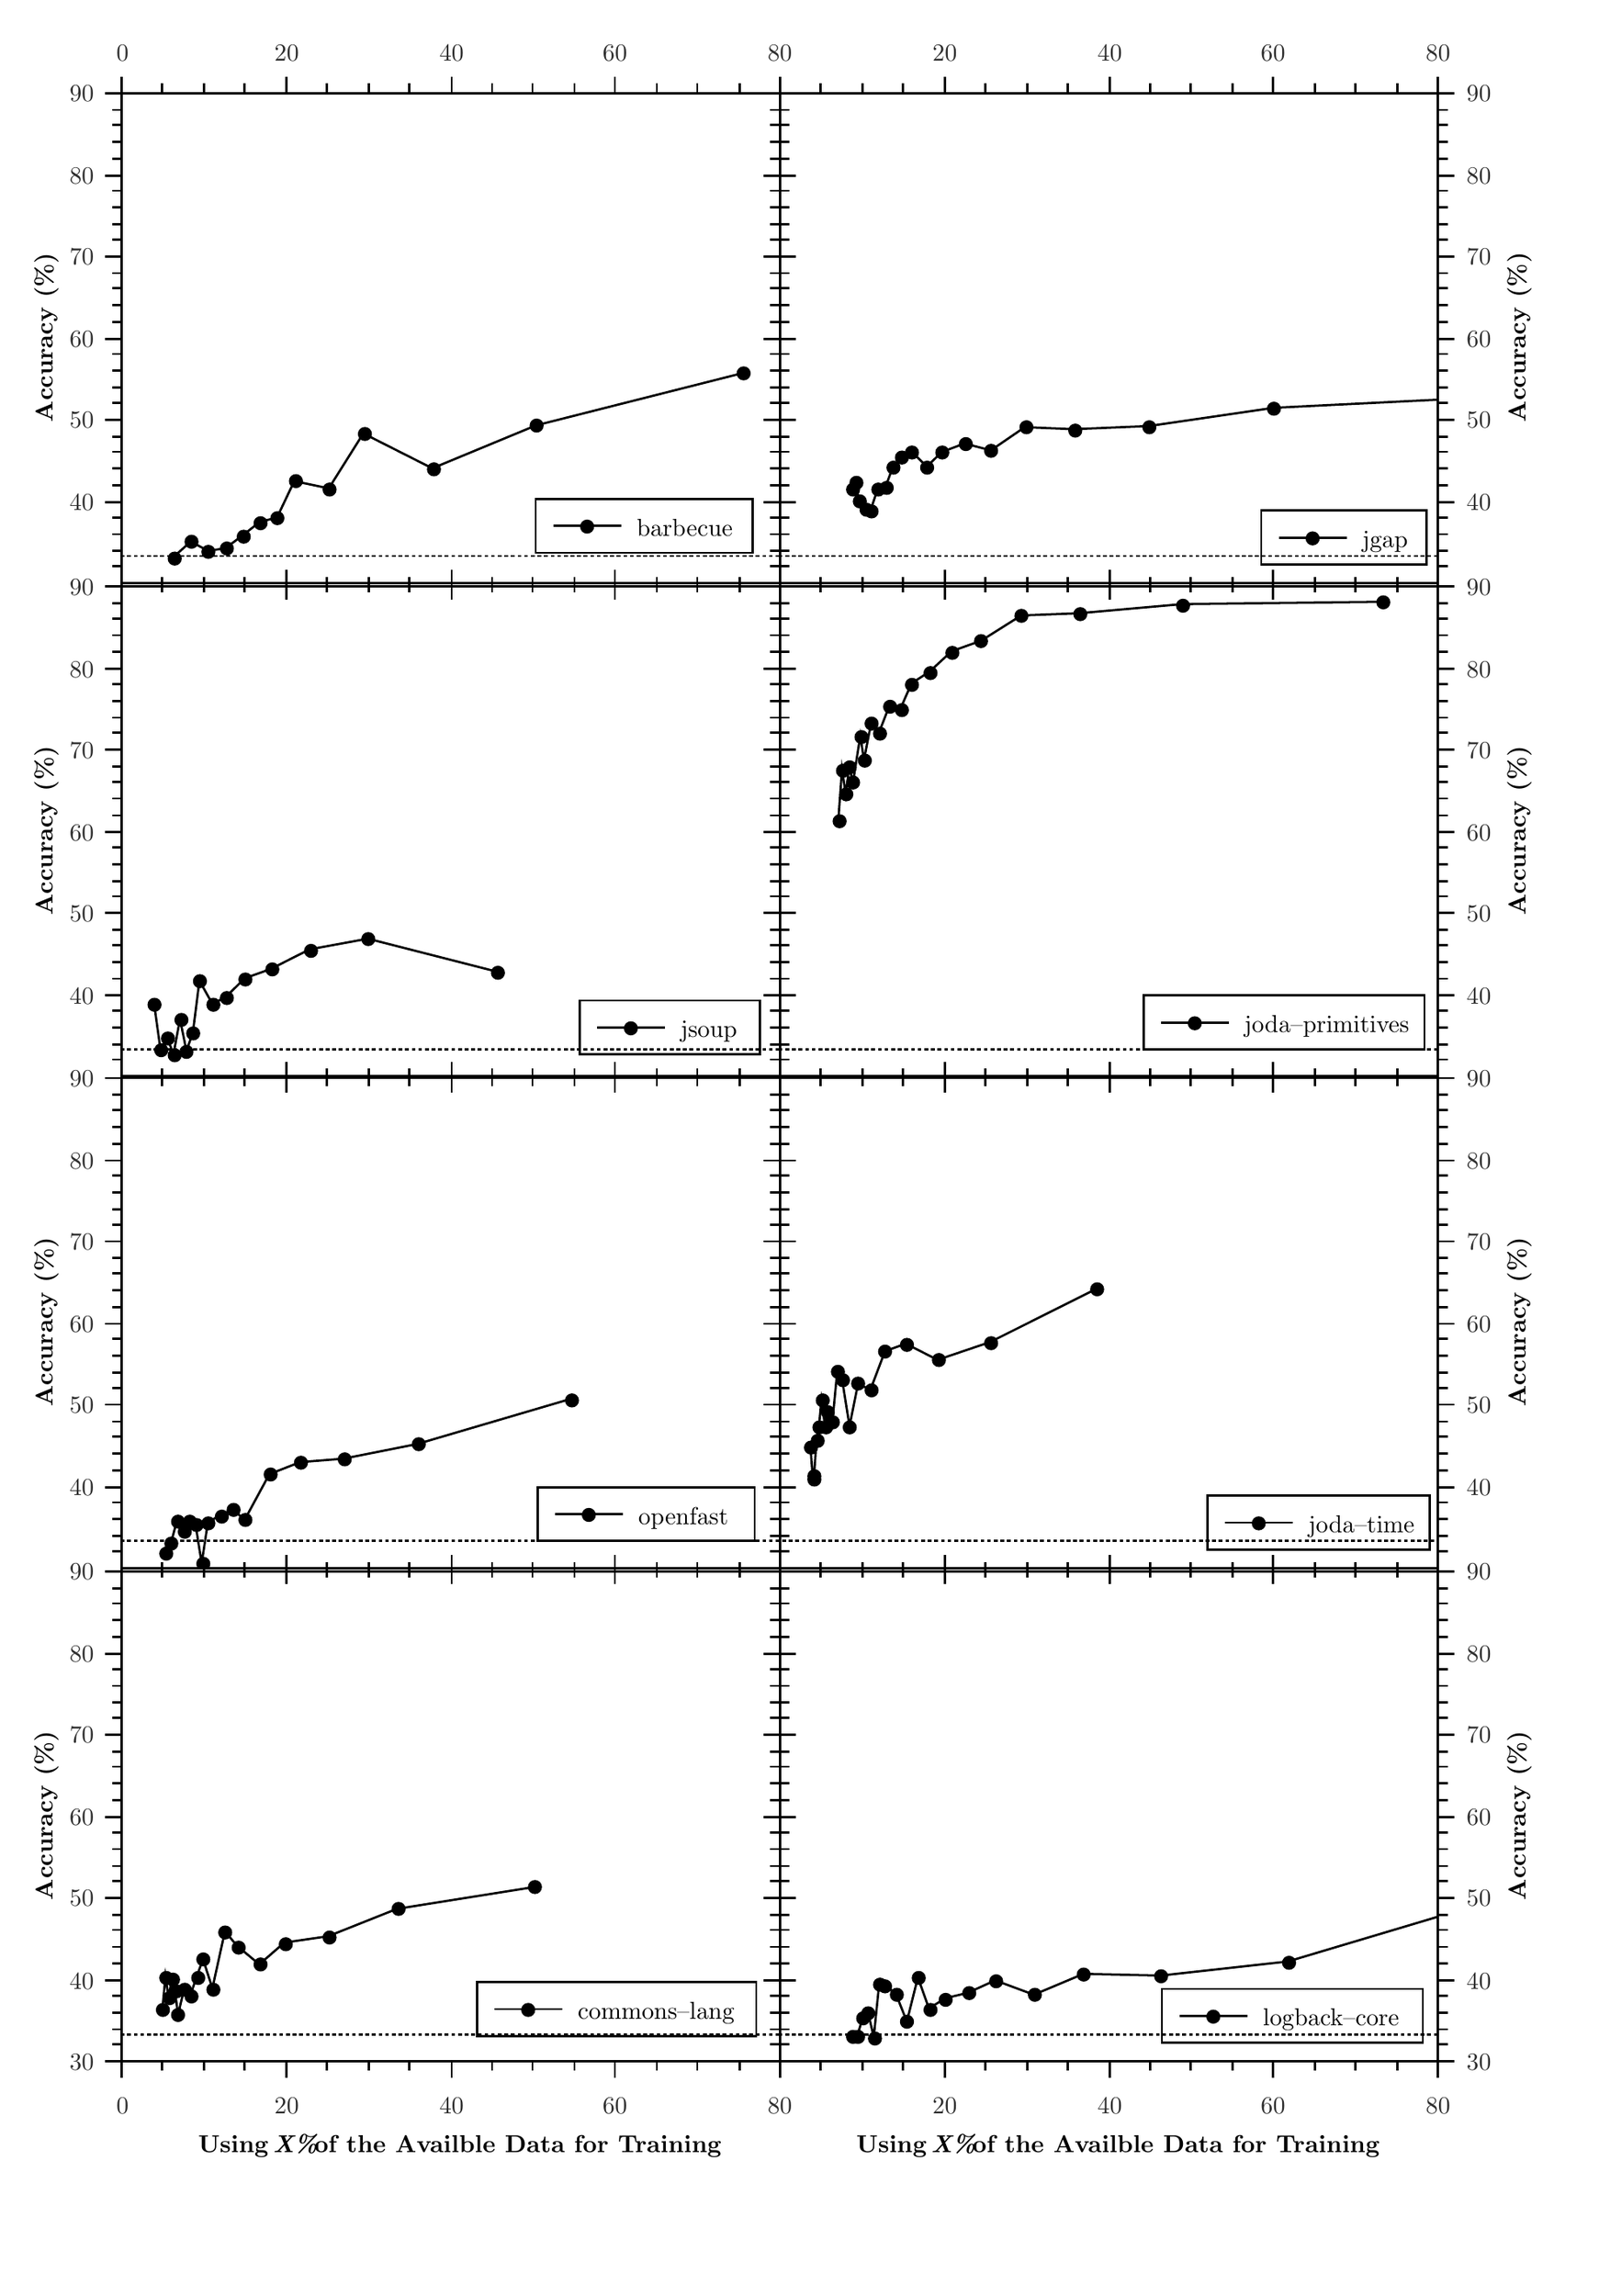
\begin{tikzpicture}{0pt}{0pt}{923pt}{1337pt}
	\clip(0pt,1337pt) -- (694.846pt,1337pt) -- (694.846pt,330.49pt) -- (0pt,330.49pt) -- (0pt,1337pt);
\begin{scope}
	\clip(44.4159pt,1305.38pt) -- (338.766pt,1305.38pt) -- (338.766pt,1086.31pt) -- (44.4159pt,1086.31pt) -- (44.4159pt,1305.38pt);
	\color[rgb]{0,0,0}
	\draw[line width=1pt, line join=miter, line cap=rect](322.299pt,1180.2pt) -- (229.671pt,1156.77pt) -- (183.357pt,1137.59pt) -- (152.481pt,1153.19pt) -- (137.043pt,1128.63pt) -- (121.606pt,1131.87pt) -- (113.887pt,1115.59pt) -- (106.168pt,1113.62pt) -- (98.4487pt,1107.56pt) -- (90.7297pt,1101.79pt) -- (83.0107pt,1100.72pt) -- (75.2918pt,1104.85pt) -- (67.5728pt,1097.89pt);
	\color[rgb]{0,0,0}
	\fill(322.58pt,1180.04pt) ellipse (2.63484pt and 2.63484pt);
	\draw[line width=1pt, line join=miter, line cap=rect](322.58pt,1180.04pt) ellipse (2.63484pt and 2.63484pt);
	\fill(229.984pt,1156.7pt) ellipse (2.63484pt and 2.63484pt);
	\draw[line width=1pt, line join=miter, line cap=rect](229.984pt,1156.7pt) ellipse (2.63484pt and 2.63484pt);
	\fill(184.063pt,1137.13pt) ellipse (2.63484pt and 2.63484pt);
	\draw[line width=1pt, line join=miter, line cap=rect](184.063pt,1137.13pt) ellipse (2.63484pt and 2.63484pt);
	\fill(153.197pt,1152.94pt) ellipse (2.63484pt and 2.63484pt);
	\draw[line width=1pt, line join=miter, line cap=rect](153.197pt,1152.94pt) ellipse (2.63484pt and 2.63484pt);
	\fill(137.388pt,1128.09pt) ellipse (2.63484pt and 2.63484pt);
	\draw[line width=1pt, line join=miter, line cap=rect](137.388pt,1128.09pt) ellipse (2.63484pt and 2.63484pt);
	\fill(122.332pt,1131.86pt) ellipse (2.63484pt and 2.63484pt);
	\draw[line width=1pt, line join=miter, line cap=rect](122.332pt,1131.86pt) ellipse (2.63484pt and 2.63484pt);
	\fill(114.051pt,1115.3pt) ellipse (2.63484pt and 2.63484pt);
	\draw[line width=1pt, line join=miter, line cap=rect](114.051pt,1115.3pt) ellipse (2.63484pt and 2.63484pt);
	\fill(106.523pt,1113.04pt) ellipse (2.63484pt and 2.63484pt);
	\draw[line width=1pt, line join=miter, line cap=rect](106.523pt,1113.04pt) ellipse (2.63484pt and 2.63484pt);
	\fill(98.9948pt,1107.02pt) ellipse (2.63484pt and 2.63484pt);
	\draw[line width=1pt, line join=miter, line cap=rect](98.9948pt,1107.02pt) ellipse (2.63484pt and 2.63484pt);
	\fill(91.4667pt,1101.75pt) ellipse (2.63484pt and 2.63484pt);
	\draw[line width=1pt, line join=miter, line cap=rect](91.4667pt,1101.75pt) ellipse (2.63484pt and 2.63484pt);
	\fill(83.1858pt,1100.24pt) ellipse (2.63484pt and 2.63484pt);
	\draw[line width=1pt, line join=miter, line cap=rect](83.1858pt,1100.24pt) ellipse (2.63484pt and 2.63484pt);
	\fill(75.6577pt,1104.76pt) ellipse (2.63484pt and 2.63484pt);
	\draw[line width=1pt, line join=miter, line cap=rect](75.6577pt,1104.76pt) ellipse (2.63484pt and 2.63484pt);
	\fill(68.1295pt,1097.23pt) ellipse (2.63484pt and 2.63484pt);
	\draw[line width=1pt, line join=miter, line cap=rect](68.1295pt,1097.23pt) ellipse (2.63484pt and 2.63484pt);
	\draw[line width=1pt, dash pattern=on 0.024cm off 0.08cm, dash phase=0pt, line join=miter, line cap=rect](44.4159pt,1098.36pt) -- (412.541pt,1098.36pt);
\end{scope}
\begin{scope}
	\color[rgb]{0,0,0}
	\pgftext[center, base, at={\pgfpoint{13.5506pt}{1196.22pt}},rotate=90]{\fontsize{11}{0}\selectfont{\textbf{Accuracy (\%)}}}
	\color[rgb]{0.172549,0.172549,0.172549}
	\pgftext[center, base, at={\pgfpoint{26.5719pt}{1118.68pt}}]{\fontsize{11}{0}\selectfont{40}}
	\pgftext[center, base, at={\pgfpoint{26.5719pt}{1155.57pt}}]{\fontsize{11}{0}\selectfont{50}}
	\pgftext[center, base, at={\pgfpoint{26.5719pt}{1191.71pt}}]{\fontsize{11}{0}\selectfont{60}}
	\pgftext[center, base, at={\pgfpoint{26.5719pt}{1228.6pt}}]{\fontsize{11}{0}\selectfont{70}}
	\pgftext[center, base, at={\pgfpoint{26.5719pt}{1264.73pt}}]{\fontsize{11}{0}\selectfont{80}}
	\pgftext[center, base, at={\pgfpoint{26.5719pt}{1301.62pt}}]{\fontsize{11}{0}\selectfont{90}}
	\color[rgb]{0,0,0}
	\draw[line width=1pt, line join=bevel, line cap=rect](44.4159pt,1093.84pt) -- (40.6519pt,1093.84pt);
	\draw[line width=1pt, line join=bevel, line cap=rect](44.4159pt,1100.62pt) -- (40.6519pt,1100.62pt);
	\draw[line width=1pt, line join=bevel, line cap=rect](44.4159pt,1108.14pt) -- (40.6519pt,1108.14pt);
	\draw[line width=1pt, line join=bevel, line cap=rect](44.4159pt,1115.67pt) -- (40.6519pt,1115.67pt);
	\draw[line width=1pt, line join=bevel, line cap=rect](44.4159pt,1129.98pt) -- (40.6519pt,1129.98pt);
	\draw[line width=1pt, line join=bevel, line cap=rect](44.4159pt,1137.5pt) -- (40.6519pt,1137.5pt);
	\draw[line width=1pt, line join=bevel, line cap=rect](44.4159pt,1145.03pt) -- (40.6519pt,1145.03pt);
	\draw[line width=1pt, line join=bevel, line cap=rect](44.4159pt,1151.81pt) -- (40.6519pt,1151.81pt);
	\draw[line width=1pt, line join=bevel, line cap=rect](44.4159pt,1166.86pt) -- (40.6519pt,1166.86pt);
	\draw[line width=1pt, line join=bevel, line cap=rect](44.4159pt,1173.64pt) -- (40.6519pt,1173.64pt);
	\draw[line width=1pt, line join=bevel, line cap=rect](44.4159pt,1181.17pt) -- (40.6519pt,1181.17pt);
	\draw[line width=1pt, line join=bevel, line cap=rect](44.4159pt,1188.7pt) -- (40.6519pt,1188.7pt);
	\draw[line width=1pt, line join=bevel, line cap=rect](44.4159pt,1203pt) -- (40.6519pt,1203pt);
	\draw[line width=1pt, line join=bevel, line cap=rect](44.4159pt,1210.53pt) -- (40.6519pt,1210.53pt);
	\draw[line width=1pt, line join=bevel, line cap=rect](44.4159pt,1218.06pt) -- (40.6519pt,1218.06pt);
	\draw[line width=1pt, line join=bevel, line cap=rect](44.4159pt,1224.83pt) -- (40.6519pt,1224.83pt);
	\draw[line width=1pt, line join=bevel, line cap=rect](44.4159pt,1239.89pt) -- (40.6519pt,1239.89pt);
	\draw[line width=1pt, line join=bevel, line cap=rect](44.4159pt,1246.66pt) -- (40.6519pt,1246.66pt);
	\draw[line width=1pt, line join=bevel, line cap=rect](44.4159pt,1254.19pt) -- (40.6519pt,1254.19pt);
	\draw[line width=1pt, line join=bevel, line cap=rect](44.4159pt,1261.72pt) -- (40.6519pt,1261.72pt);
	\draw[line width=1pt, line join=bevel, line cap=rect](44.4159pt,1276.02pt) -- (40.6519pt,1276.02pt);
	\draw[line width=1pt, line join=bevel, line cap=rect](44.4159pt,1283.55pt) -- (40.6519pt,1283.55pt);
	\draw[line width=1pt, line join=bevel, line cap=rect](44.4159pt,1291.08pt) -- (40.6519pt,1291.08pt);
	\draw[line width=1pt, line join=bevel, line cap=rect](44.4159pt,1297.85pt) -- (40.6519pt,1297.85pt);
	\draw[line width=1pt, line join=bevel, line cap=rect](44.4159pt,1122.45pt) -- (37.6406pt,1122.45pt);
	\draw[line width=1pt, line join=bevel, line cap=rect](44.4159pt,1159.34pt) -- (37.6406pt,1159.34pt);
	\draw[line width=1pt, line join=bevel, line cap=rect](44.4159pt,1195.47pt) -- (37.6406pt,1195.47pt);
	\draw[line width=1pt, line join=bevel, line cap=rect](44.4159pt,1232.36pt) -- (37.6406pt,1232.36pt);
	\draw[line width=1pt, line join=bevel, line cap=rect](44.4159pt,1268.49pt) -- (37.6406pt,1268.49pt);
	\draw[line width=1pt, line join=bevel, line cap=rect](44.4159pt,1305.38pt) -- (37.6406pt,1305.38pt);
	\draw[line width=1pt, line join=bevel, line cap=rect](44.4159pt,1305.38pt) -- (44.4159pt,1086.31pt);
	\draw[line width=1pt, line join=bevel, line cap=rect](338.766pt,1093.84pt) -- (342.53pt,1093.84pt);
	\draw[line width=1pt, line join=bevel, line cap=rect](338.766pt,1100.62pt) -- (342.53pt,1100.62pt);
	\draw[line width=1pt, line join=bevel, line cap=rect](338.766pt,1108.14pt) -- (342.53pt,1108.14pt);
	\draw[line width=1pt, line join=bevel, line cap=rect](338.766pt,1115.67pt) -- (342.53pt,1115.67pt);
	\draw[line width=1pt, line join=bevel, line cap=rect](338.766pt,1129.98pt) -- (342.53pt,1129.98pt);
	\draw[line width=1pt, line join=bevel, line cap=rect](338.766pt,1137.5pt) -- (342.53pt,1137.5pt);
	\draw[line width=1pt, line join=bevel, line cap=rect](338.766pt,1145.03pt) -- (342.53pt,1145.03pt);
	\draw[line width=1pt, line join=bevel, line cap=rect](338.766pt,1151.81pt) -- (342.53pt,1151.81pt);
	\draw[line width=1pt, line join=bevel, line cap=rect](338.766pt,1166.86pt) -- (342.53pt,1166.86pt);
	\draw[line width=1pt, line join=bevel, line cap=rect](338.766pt,1173.64pt) -- (342.53pt,1173.64pt);
	\draw[line width=1pt, line join=bevel, line cap=rect](338.766pt,1181.17pt) -- (342.53pt,1181.17pt);
	\draw[line width=1pt, line join=bevel, line cap=rect](338.766pt,1188.7pt) -- (342.53pt,1188.7pt);
	\draw[line width=1pt, line join=bevel, line cap=rect](338.766pt,1203pt) -- (342.53pt,1203pt);
	\draw[line width=1pt, line join=bevel, line cap=rect](338.766pt,1210.53pt) -- (342.53pt,1210.53pt);
	\draw[line width=1pt, line join=bevel, line cap=rect](338.766pt,1218.06pt) -- (342.53pt,1218.06pt);
	\draw[line width=1pt, line join=bevel, line cap=rect](338.766pt,1224.83pt) -- (342.53pt,1224.83pt);
	\draw[line width=1pt, line join=bevel, line cap=rect](338.766pt,1239.89pt) -- (342.53pt,1239.89pt);
	\draw[line width=1pt, line join=bevel, line cap=rect](338.766pt,1246.66pt) -- (342.53pt,1246.66pt);
	\draw[line width=1pt, line join=bevel, line cap=rect](338.766pt,1254.19pt) -- (342.53pt,1254.19pt);
	\draw[line width=1pt, line join=bevel, line cap=rect](338.766pt,1261.72pt) -- (342.53pt,1261.72pt);
	\draw[line width=1pt, line join=bevel, line cap=rect](338.766pt,1276.02pt) -- (342.53pt,1276.02pt);
	\draw[line width=1pt, line join=bevel, line cap=rect](338.766pt,1283.55pt) -- (342.53pt,1283.55pt);
	\draw[line width=1pt, line join=bevel, line cap=rect](338.766pt,1291.08pt) -- (342.53pt,1291.08pt);
	\draw[line width=1pt, line join=bevel, line cap=rect](338.766pt,1297.85pt) -- (342.53pt,1297.85pt);
	\draw[line width=1pt, line join=bevel, line cap=rect](338.766pt,1086.31pt) -- (345.541pt,1086.31pt);
	\draw[line width=1pt, line join=bevel, line cap=rect](338.766pt,1122.45pt) -- (345.541pt,1122.45pt);
	\draw[line width=1pt, line join=bevel, line cap=rect](338.766pt,1159.34pt) -- (345.541pt,1159.34pt);
	\draw[line width=1pt, line join=bevel, line cap=rect](338.766pt,1195.47pt) -- (345.541pt,1195.47pt);
	\draw[line width=1pt, line join=bevel, line cap=rect](338.766pt,1232.36pt) -- (345.541pt,1232.36pt);
	\draw[line width=1pt, line join=bevel, line cap=rect](338.766pt,1268.49pt) -- (345.541pt,1268.49pt);
	\draw[line width=1pt, line join=bevel, line cap=rect](338.766pt,1305.38pt) -- (345.541pt,1305.38pt);
	\draw[line width=1pt, line join=bevel, line cap=rect](338.766pt,1305.38pt) -- (338.766pt,1086.31pt);
	\draw[line width=1pt, line join=bevel, line cap=rect](62.4834pt,1086.31pt) -- (62.4834pt,1082.55pt);
	\draw[line width=1pt, line join=bevel, line cap=rect](99.3713pt,1086.31pt) -- (99.3713pt,1082.55pt);
	\draw[line width=1pt, line join=bevel, line cap=rect](136.259pt,1086.31pt) -- (136.259pt,1082.55pt);
	\draw[line width=1pt, line join=bevel, line cap=rect](173.147pt,1086.31pt) -- (173.147pt,1082.55pt);
	\draw[line width=1pt, line join=bevel, line cap=rect](210.035pt,1086.31pt) -- (210.035pt,1082.55pt);
	\draw[line width=1pt, line join=bevel, line cap=rect](246.922pt,1086.31pt) -- (246.922pt,1082.55pt);
	\draw[line width=1pt, line join=bevel, line cap=rect](283.81pt,1086.31pt) -- (283.81pt,1082.55pt);
	\draw[line width=1pt, line join=bevel, line cap=rect](320.698pt,1086.31pt) -- (320.698pt,1082.55pt);
	\draw[line width=1pt, line join=bevel, line cap=rect](81.3037pt,1086.31pt) -- (81.3037pt,1082.55pt);
	\draw[line width=1pt, line join=bevel, line cap=rect](155.079pt,1086.31pt) -- (155.079pt,1082.55pt);
	\draw[line width=1pt, line join=bevel, line cap=rect](228.102pt,1086.31pt) -- (228.102pt,1082.55pt);
	\draw[line width=1pt, line join=bevel, line cap=rect](301.878pt,1086.31pt) -- (301.878pt,1082.55pt);
	\draw[line width=1pt, line join=bevel, line cap=rect](44.4159pt,1086.31pt) -- (44.4159pt,1079.54pt);
	\draw[line width=1pt, line join=bevel, line cap=rect](118.192pt,1086.31pt) -- (118.192pt,1079.54pt);
	\draw[line width=1pt, line join=bevel, line cap=rect](191.967pt,1086.31pt) -- (191.967pt,1079.54pt);
	\draw[line width=1pt, line join=bevel, line cap=rect](264.99pt,1086.31pt) -- (264.99pt,1079.54pt);
	\draw[line width=1pt, line join=bevel, line cap=rect](338.766pt,1086.31pt) -- (338.766pt,1079.54pt);
	\draw[line width=1pt, line join=bevel, line cap=rect](44.4159pt,1086.31pt) -- (338.766pt,1086.31pt);
	\color[rgb]{0.172549,0.172549,0.172549}
	\pgftext[center, base, at={\pgfpoint{44.7865pt}{1319.69pt}}]{\fontsize{11}{0}\selectfont{0}}
	\pgftext[center, base, at={\pgfpoint{118.192pt}{1319.69pt}}]{\fontsize{11}{0}\selectfont{20}}
	\pgftext[center, base, at={\pgfpoint{191.967pt}{1319.69pt}}]{\fontsize{11}{0}\selectfont{40}}
	\pgftext[center, base, at={\pgfpoint{264.99pt}{1319.69pt}}]{\fontsize{11}{0}\selectfont{60}}
	\pgftext[center, base, at={\pgfpoint{338.766pt}{1319.69pt}}]{\fontsize{11}{0}\selectfont{80}}
	\color[rgb]{0,0,0}
	\draw[line width=1pt, line join=bevel, line cap=rect](62.4834pt,1305.38pt) -- (62.4834pt,1309.15pt);
	\draw[line width=1pt, line join=bevel, line cap=rect](99.3713pt,1305.38pt) -- (99.3713pt,1309.15pt);
	\draw[line width=1pt, line join=bevel, line cap=rect](136.259pt,1305.38pt) -- (136.259pt,1309.15pt);
	\draw[line width=1pt, line join=bevel, line cap=rect](173.147pt,1305.38pt) -- (173.147pt,1309.15pt);
	\draw[line width=1pt, line join=bevel, line cap=rect](210.035pt,1305.38pt) -- (210.035pt,1309.15pt);
	\draw[line width=1pt, line join=bevel, line cap=rect](246.922pt,1305.38pt) -- (246.922pt,1309.15pt);
	\draw[line width=1pt, line join=bevel, line cap=rect](283.81pt,1305.38pt) -- (283.81pt,1309.15pt);
	\draw[line width=1pt, line join=bevel, line cap=rect](320.698pt,1305.38pt) -- (320.698pt,1309.15pt);
	\draw[line width=1pt, line join=bevel, line cap=rect](81.3037pt,1305.38pt) -- (81.3037pt,1309.15pt);
	\draw[line width=1pt, line join=bevel, line cap=rect](155.079pt,1305.38pt) -- (155.079pt,1309.15pt);
	\draw[line width=1pt, line join=bevel, line cap=rect](228.102pt,1305.38pt) -- (228.102pt,1309.15pt);
	\draw[line width=1pt, line join=bevel, line cap=rect](301.878pt,1305.38pt) -- (301.878pt,1309.15pt);
	\draw[line width=1pt, line join=bevel, line cap=rect](44.4159pt,1305.38pt) -- (44.4159pt,1312.16pt);
	\draw[line width=1pt, line join=bevel, line cap=rect](118.192pt,1305.38pt) -- (118.192pt,1312.16pt);
	\draw[line width=1pt, line join=bevel, line cap=rect](191.967pt,1305.38pt) -- (191.967pt,1312.16pt);
	\draw[line width=1pt, line join=bevel, line cap=rect](264.99pt,1305.38pt) -- (264.99pt,1312.16pt);
	\draw[line width=1pt, line join=bevel, line cap=rect](338.766pt,1305.38pt) -- (338.766pt,1312.16pt);
	\draw[line width=1pt, line join=bevel, line cap=rect](44.4159pt,1305.38pt) -- (338.766pt,1305.38pt);
	\draw[line width=1pt, line join=miter, line cap=rect](229.608pt,1123.95pt) -- (326.721pt,1123.95pt) -- (326.721pt,1099.86pt) -- (229.608pt,1099.86pt) -- (229.608pt,1123.95pt);
	\draw[line width=1pt, line join=miter, line cap=rect](237.889pt,1111.91pt) -- (267.248pt,1111.91pt);
	\fill(252.569pt,1111.53pt) ellipse (2.63484pt and 2.63484pt);
	\draw[line width=1pt, line join=miter, line cap=rect](252.569pt,1111.53pt) ellipse (2.63484pt and 2.63484pt);
	\pgftext[left, base, at={\pgfpoint{274.777pt}{1107.39pt}}]{\fontsize{11}{0}\selectfont{barbecue}}
\end{scope}
\begin{scope}
	\clip(44.4159pt,1084.81pt) -- (338.766pt,1084.81pt) -- (338.766pt,865.739pt) -- (44.4159pt,865.739pt) -- (44.4159pt,1084.81pt);
	\color[rgb]{0,0,0}
	\draw[line width=1pt, line join=miter, line cap=rect](212.45pt,912.481pt) -- (154.507pt,927.275pt) -- (128.433pt,922.493pt) -- (111.05pt,913.719pt) -- (99.4616pt,909.576pt) -- (90.7702pt,901.045pt) -- (84.9759pt,898.158pt) -- (79.1816pt,908.495pt) -- (76.2845pt,885.464pt) -- (73.3874pt,877.078pt) -- (70.4902pt,891.318pt) -- (67.5931pt,875.711pt) -- (64.6959pt,883.082pt) -- (61.7988pt,877.44pt) -- (58.9017pt,898.26pt);
	\color[rgb]{0,0,0}
	\fill(212.67pt,912.037pt) ellipse (2.63484pt and 2.63484pt);
	\draw[line width=1pt, line join=miter, line cap=rect](212.67pt,912.037pt) ellipse (2.63484pt and 2.63484pt);
	\fill(154.703pt,927.094pt) ellipse (2.63484pt and 2.63484pt);
	\draw[line width=1pt, line join=miter, line cap=rect](154.703pt,927.094pt) ellipse (2.63484pt and 2.63484pt);
	\fill(129.107pt,921.824pt) ellipse (2.63484pt and 2.63484pt);
	\draw[line width=1pt, line join=miter, line cap=rect](129.107pt,921.824pt) ellipse (2.63484pt and 2.63484pt);
	\fill(111.793pt,913.543pt) ellipse (2.63484pt and 2.63484pt);
	\draw[line width=1pt, line join=miter, line cap=rect](111.793pt,913.543pt) ellipse (2.63484pt and 2.63484pt);
	\fill(99.7477pt,909.026pt) ellipse (2.63484pt and 2.63484pt);
	\draw[line width=1pt, line join=miter, line cap=rect](99.7477pt,909.026pt) ellipse (2.63484pt and 2.63484pt);
	\fill(91.4667pt,900.745pt) ellipse (2.63484pt and 2.63484pt);
	\draw[line width=1pt, line join=miter, line cap=rect](91.4667pt,900.745pt) ellipse (2.63484pt and 2.63484pt);
	\fill(85.4442pt,897.734pt) ellipse (2.63484pt and 2.63484pt);
	\draw[line width=1pt, line join=miter, line cap=rect](85.4442pt,897.734pt) ellipse (2.63484pt and 2.63484pt);
	\fill(79.4217pt,908.273pt) ellipse (2.63484pt and 2.63484pt);
	\draw[line width=1pt, line join=miter, line cap=rect](79.4217pt,908.273pt) ellipse (2.63484pt and 2.63484pt);
	\fill(76.4105pt,884.936pt) ellipse (2.63484pt and 2.63484pt);
	\draw[line width=1pt, line join=miter, line cap=rect](76.4105pt,884.936pt) ellipse (2.63484pt and 2.63484pt);
	\fill(73.3992pt,876.655pt) ellipse (2.63484pt and 2.63484pt);
	\draw[line width=1pt, line join=miter, line cap=rect](73.3992pt,876.655pt) ellipse (2.63484pt and 2.63484pt);
	\fill(71.1408pt,890.959pt) ellipse (2.63484pt and 2.63484pt);
	\draw[line width=1pt, line join=miter, line cap=rect](71.1408pt,890.959pt) ellipse (2.63484pt and 2.63484pt);
	\fill(68.1295pt,875.15pt) ellipse (2.63484pt and 2.63484pt);
	\draw[line width=1pt, line join=miter, line cap=rect](68.1295pt,875.15pt) ellipse (2.63484pt and 2.63484pt);
	\fill(65.1183pt,882.678pt) ellipse (2.63484pt and 2.63484pt);
	\draw[line width=1pt, line join=miter, line cap=rect](65.1183pt,882.678pt) ellipse (2.63484pt and 2.63484pt);
	\fill(62.107pt,877.408pt) ellipse (2.63484pt and 2.63484pt);
	\draw[line width=1pt, line join=miter, line cap=rect](62.107pt,877.408pt) ellipse (2.63484pt and 2.63484pt);
	\fill(59.0958pt,897.734pt) ellipse (2.63484pt and 2.63484pt);
	\draw[line width=1pt, line join=miter, line cap=rect](59.0958pt,897.734pt) ellipse (2.63484pt and 2.63484pt);
	\draw[line width=1pt, dash pattern=on 0.024cm off 0.08cm, dash phase=0pt, line join=miter, line cap=rect](44.4159pt,877.784pt) -- (412.541pt,877.784pt);
\end{scope}
\begin{scope}
	\color[rgb]{0,0,0}
	\pgftext[center, base, at={\pgfpoint{13.5506pt}{975.644pt}},rotate=90]{\fontsize{11}{0}\selectfont{\textbf{Accuracy (\%)}}}
	\color[rgb]{0.172549,0.172549,0.172549}
	\pgftext[center, base, at={\pgfpoint{26.5719pt}{898.11pt}}]{\fontsize{11}{0}\selectfont{40}}
	\pgftext[center, base, at={\pgfpoint{26.5719pt}{934.998pt}}]{\fontsize{11}{0}\selectfont{50}}
	\pgftext[center, base, at={\pgfpoint{26.5719pt}{971.133pt}}]{\fontsize{11}{0}\selectfont{60}}
	\pgftext[center, base, at={\pgfpoint{26.5719pt}{1008.02pt}}]{\fontsize{11}{0}\selectfont{70}}
	\pgftext[center, base, at={\pgfpoint{26.5719pt}{1044.16pt}}]{\fontsize{11}{0}\selectfont{80}}
	\pgftext[center, base, at={\pgfpoint{26.5719pt}{1081.04pt}}]{\fontsize{11}{0}\selectfont{90}}
	\color[rgb]{0,0,0}
	\draw[line width=1pt, line join=bevel, line cap=rect](44.4159pt,873.267pt) -- (40.6519pt,873.267pt);
	\draw[line width=1pt, line join=bevel, line cap=rect](44.4159pt,880.043pt) -- (40.6519pt,880.043pt);
	\draw[line width=1pt, line join=bevel, line cap=rect](44.4159pt,887.571pt) -- (40.6519pt,887.571pt);
	\draw[line width=1pt, line join=bevel, line cap=rect](44.4159pt,895.099pt) -- (40.6519pt,895.099pt);
	\draw[line width=1pt, line join=bevel, line cap=rect](44.4159pt,909.402pt) -- (40.6519pt,909.402pt);
	\draw[line width=1pt, line join=bevel, line cap=rect](44.4159pt,916.931pt) -- (40.6519pt,916.931pt);
	\draw[line width=1pt, line join=bevel, line cap=rect](44.4159pt,924.459pt) -- (40.6519pt,924.459pt);
	\draw[line width=1pt, line join=bevel, line cap=rect](44.4159pt,931.234pt) -- (40.6519pt,931.234pt);
	\draw[line width=1pt, line join=bevel, line cap=rect](44.4159pt,946.29pt) -- (40.6519pt,946.29pt);
	\draw[line width=1pt, line join=bevel, line cap=rect](44.4159pt,953.066pt) -- (40.6519pt,953.066pt);
	\draw[line width=1pt, line join=bevel, line cap=rect](44.4159pt,960.594pt) -- (40.6519pt,960.594pt);
	\draw[line width=1pt, line join=bevel, line cap=rect](44.4159pt,968.122pt) -- (40.6519pt,968.122pt);
	\draw[line width=1pt, line join=bevel, line cap=rect](44.4159pt,982.425pt) -- (40.6519pt,982.425pt);
	\draw[line width=1pt, line join=bevel, line cap=rect](44.4159pt,989.953pt) -- (40.6519pt,989.953pt);
	\draw[line width=1pt, line join=bevel, line cap=rect](44.4159pt,997.482pt) -- (40.6519pt,997.482pt);
	\draw[line width=1pt, line join=bevel, line cap=rect](44.4159pt,1004.26pt) -- (40.6519pt,1004.26pt);
	\draw[line width=1pt, line join=bevel, line cap=rect](44.4159pt,1019.31pt) -- (40.6519pt,1019.31pt);
	\draw[line width=1pt, line join=bevel, line cap=rect](44.4159pt,1026.09pt) -- (40.6519pt,1026.09pt);
	\draw[line width=1pt, line join=bevel, line cap=rect](44.4159pt,1033.62pt) -- (40.6519pt,1033.62pt);
	\draw[line width=1pt, line join=bevel, line cap=rect](44.4159pt,1041.14pt) -- (40.6519pt,1041.14pt);
	\draw[line width=1pt, line join=bevel, line cap=rect](44.4159pt,1055.45pt) -- (40.6519pt,1055.45pt);
	\draw[line width=1pt, line join=bevel, line cap=rect](44.4159pt,1062.98pt) -- (40.6519pt,1062.98pt);
	\draw[line width=1pt, line join=bevel, line cap=rect](44.4159pt,1070.5pt) -- (40.6519pt,1070.5pt);
	\draw[line width=1pt, line join=bevel, line cap=rect](44.4159pt,1077.28pt) -- (40.6519pt,1077.28pt);
	\draw[line width=1pt, line join=bevel, line cap=rect](44.4159pt,901.874pt) -- (37.6406pt,901.874pt);
	\draw[line width=1pt, line join=bevel, line cap=rect](44.4159pt,938.762pt) -- (37.6406pt,938.762pt);
	\draw[line width=1pt, line join=bevel, line cap=rect](44.4159pt,974.897pt) -- (37.6406pt,974.897pt);
	\draw[line width=1pt, line join=bevel, line cap=rect](44.4159pt,1011.79pt) -- (37.6406pt,1011.79pt);
	\draw[line width=1pt, line join=bevel, line cap=rect](44.4159pt,1047.92pt) -- (37.6406pt,1047.92pt);
	\draw[line width=1pt, line join=bevel, line cap=rect](44.4159pt,1084.81pt) -- (37.6406pt,1084.81pt);
	\draw[line width=1pt, line join=bevel, line cap=rect](44.4159pt,1084.81pt) -- (44.4159pt,865.739pt);
	\draw[line width=1pt, line join=bevel, line cap=rect](338.766pt,873.267pt) -- (342.53pt,873.267pt);
	\draw[line width=1pt, line join=bevel, line cap=rect](338.766pt,880.043pt) -- (342.53pt,880.043pt);
	\draw[line width=1pt, line join=bevel, line cap=rect](338.766pt,887.571pt) -- (342.53pt,887.571pt);
	\draw[line width=1pt, line join=bevel, line cap=rect](338.766pt,895.099pt) -- (342.53pt,895.099pt);
	\draw[line width=1pt, line join=bevel, line cap=rect](338.766pt,909.402pt) -- (342.53pt,909.402pt);
	\draw[line width=1pt, line join=bevel, line cap=rect](338.766pt,916.931pt) -- (342.53pt,916.931pt);
	\draw[line width=1pt, line join=bevel, line cap=rect](338.766pt,924.459pt) -- (342.53pt,924.459pt);
	\draw[line width=1pt, line join=bevel, line cap=rect](338.766pt,931.234pt) -- (342.53pt,931.234pt);
	\draw[line width=1pt, line join=bevel, line cap=rect](338.766pt,946.29pt) -- (342.53pt,946.29pt);
	\draw[line width=1pt, line join=bevel, line cap=rect](338.766pt,953.066pt) -- (342.53pt,953.066pt);
	\draw[line width=1pt, line join=bevel, line cap=rect](338.766pt,960.594pt) -- (342.53pt,960.594pt);
	\draw[line width=1pt, line join=bevel, line cap=rect](338.766pt,968.122pt) -- (342.53pt,968.122pt);
	\draw[line width=1pt, line join=bevel, line cap=rect](338.766pt,982.425pt) -- (342.53pt,982.425pt);
	\draw[line width=1pt, line join=bevel, line cap=rect](338.766pt,989.953pt) -- (342.53pt,989.953pt);
	\draw[line width=1pt, line join=bevel, line cap=rect](338.766pt,997.482pt) -- (342.53pt,997.482pt);
	\draw[line width=1pt, line join=bevel, line cap=rect](338.766pt,1004.26pt) -- (342.53pt,1004.26pt);
	\draw[line width=1pt, line join=bevel, line cap=rect](338.766pt,1019.31pt) -- (342.53pt,1019.31pt);
	\draw[line width=1pt, line join=bevel, line cap=rect](338.766pt,1026.09pt) -- (342.53pt,1026.09pt);
	\draw[line width=1pt, line join=bevel, line cap=rect](338.766pt,1033.62pt) -- (342.53pt,1033.62pt);
	\draw[line width=1pt, line join=bevel, line cap=rect](338.766pt,1041.14pt) -- (342.53pt,1041.14pt);
	\draw[line width=1pt, line join=bevel, line cap=rect](338.766pt,1055.45pt) -- (342.53pt,1055.45pt);
	\draw[line width=1pt, line join=bevel, line cap=rect](338.766pt,1062.98pt) -- (342.53pt,1062.98pt);
	\draw[line width=1pt, line join=bevel, line cap=rect](338.766pt,1070.5pt) -- (342.53pt,1070.5pt);
	\draw[line width=1pt, line join=bevel, line cap=rect](338.766pt,1077.28pt) -- (342.53pt,1077.28pt);
	\draw[line width=1pt, line join=bevel, line cap=rect](338.766pt,865.739pt) -- (345.541pt,865.739pt);
	\draw[line width=1pt, line join=bevel, line cap=rect](338.766pt,901.874pt) -- (345.541pt,901.874pt);
	\draw[line width=1pt, line join=bevel, line cap=rect](338.766pt,938.762pt) -- (345.541pt,938.762pt);
	\draw[line width=1pt, line join=bevel, line cap=rect](338.766pt,974.897pt) -- (345.541pt,974.897pt);
	\draw[line width=1pt, line join=bevel, line cap=rect](338.766pt,1011.79pt) -- (345.541pt,1011.79pt);
	\draw[line width=1pt, line join=bevel, line cap=rect](338.766pt,1047.92pt) -- (345.541pt,1047.92pt);
	\draw[line width=1pt, line join=bevel, line cap=rect](338.766pt,1084.81pt) -- (345.541pt,1084.81pt);
	\draw[line width=1pt, line join=bevel, line cap=rect](338.766pt,1084.81pt) -- (338.766pt,865.739pt);
	\draw[line width=1pt, line join=bevel, line cap=rect](62.4834pt,865.739pt) -- (62.4834pt,861.975pt);
	\draw[line width=1pt, line join=bevel, line cap=rect](99.3713pt,865.739pt) -- (99.3713pt,861.975pt);
	\draw[line width=1pt, line join=bevel, line cap=rect](136.259pt,865.739pt) -- (136.259pt,861.975pt);
	\draw[line width=1pt, line join=bevel, line cap=rect](173.147pt,865.739pt) -- (173.147pt,861.975pt);
	\draw[line width=1pt, line join=bevel, line cap=rect](210.035pt,865.739pt) -- (210.035pt,861.975pt);
	\draw[line width=1pt, line join=bevel, line cap=rect](246.922pt,865.739pt) -- (246.922pt,861.975pt);
	\draw[line width=1pt, line join=bevel, line cap=rect](283.81pt,865.739pt) -- (283.81pt,861.975pt);
	\draw[line width=1pt, line join=bevel, line cap=rect](320.698pt,865.739pt) -- (320.698pt,861.975pt);
	\draw[line width=1pt, line join=bevel, line cap=rect](81.3037pt,865.739pt) -- (81.3037pt,861.975pt);
	\draw[line width=1pt, line join=bevel, line cap=rect](155.079pt,865.739pt) -- (155.079pt,861.975pt);
	\draw[line width=1pt, line join=bevel, line cap=rect](228.102pt,865.739pt) -- (228.102pt,861.975pt);
	\draw[line width=1pt, line join=bevel, line cap=rect](301.878pt,865.739pt) -- (301.878pt,861.975pt);
	\draw[line width=1pt, line join=bevel, line cap=rect](44.4159pt,865.739pt) -- (44.4159pt,858.964pt);
	\draw[line width=1pt, line join=bevel, line cap=rect](118.192pt,865.739pt) -- (118.192pt,858.964pt);
	\draw[line width=1pt, line join=bevel, line cap=rect](191.967pt,865.739pt) -- (191.967pt,858.964pt);
	\draw[line width=1pt, line join=bevel, line cap=rect](264.99pt,865.739pt) -- (264.99pt,858.964pt);
	\draw[line width=1pt, line join=bevel, line cap=rect](338.766pt,865.739pt) -- (338.766pt,858.964pt);
	\draw[line width=1pt, line join=bevel, line cap=rect](44.4159pt,865.739pt) -- (338.766pt,865.739pt);
	\draw[line width=1pt, line join=bevel, line cap=rect](62.4834pt,1084.81pt) -- (62.4834pt,1088.57pt);
	\draw[line width=1pt, line join=bevel, line cap=rect](99.3713pt,1084.81pt) -- (99.3713pt,1088.57pt);
	\draw[line width=1pt, line join=bevel, line cap=rect](136.259pt,1084.81pt) -- (136.259pt,1088.57pt);
	\draw[line width=1pt, line join=bevel, line cap=rect](173.147pt,1084.81pt) -- (173.147pt,1088.57pt);
	\draw[line width=1pt, line join=bevel, line cap=rect](210.035pt,1084.81pt) -- (210.035pt,1088.57pt);
	\draw[line width=1pt, line join=bevel, line cap=rect](246.922pt,1084.81pt) -- (246.922pt,1088.57pt);
	\draw[line width=1pt, line join=bevel, line cap=rect](283.81pt,1084.81pt) -- (283.81pt,1088.57pt);
	\draw[line width=1pt, line join=bevel, line cap=rect](320.698pt,1084.81pt) -- (320.698pt,1088.57pt);
	\draw[line width=1pt, line join=bevel, line cap=rect](81.3037pt,1084.81pt) -- (81.3037pt,1088.57pt);
	\draw[line width=1pt, line join=bevel, line cap=rect](155.079pt,1084.81pt) -- (155.079pt,1088.57pt);
	\draw[line width=1pt, line join=bevel, line cap=rect](228.102pt,1084.81pt) -- (228.102pt,1088.57pt);
	\draw[line width=1pt, line join=bevel, line cap=rect](301.878pt,1084.81pt) -- (301.878pt,1088.57pt);
	\draw[line width=1pt, line join=bevel, line cap=rect](44.4159pt,1084.81pt) -- (44.4159pt,1091.58pt);
	\draw[line width=1pt, line join=bevel, line cap=rect](118.192pt,1084.81pt) -- (118.192pt,1091.58pt);
	\draw[line width=1pt, line join=bevel, line cap=rect](191.967pt,1084.81pt) -- (191.967pt,1091.58pt);
	\draw[line width=1pt, line join=bevel, line cap=rect](264.99pt,1084.81pt) -- (264.99pt,1091.58pt);
	\draw[line width=1pt, line join=bevel, line cap=rect](338.766pt,1084.81pt) -- (338.766pt,1091.58pt);
	\draw[line width=1pt, line join=bevel, line cap=rect](44.4159pt,1084.81pt) -- (338.766pt,1084.81pt);
	\draw[line width=1pt, line join=miter, line cap=rect](249.181pt,899.616pt) -- (329.732pt,899.616pt) -- (329.732pt,875.526pt) -- (249.181pt,875.526pt) -- (249.181pt,899.616pt);
	\draw[line width=1pt, line join=miter, line cap=rect](257.462pt,887.571pt) -- (286.822pt,887.571pt);
	\fill(272.142pt,887.195pt) ellipse (2.63484pt and 2.63484pt);
	\draw[line width=1pt, line join=miter, line cap=rect](272.142pt,887.195pt) ellipse (2.63484pt and 2.63484pt);
	\pgftext[left, base, at={\pgfpoint{294.35pt}{883.054pt}}]{\fontsize{11}{0}\selectfont{jsoup}}
\end{scope}
\begin{scope}
	\clip(44.4159pt,864.987pt) -- (338.766pt,864.987pt) -- (338.766pt,645.918pt) -- (44.4159pt,645.918pt) -- (44.4159pt,864.987pt);
	\color[rgb]{0,0,0}
	\draw[line width=1pt, line join=miter, line cap=rect](245.359pt,721.549pt) -- (176.543pt,701.325pt) -- (143.511pt,694.766pt) -- (124.243pt,693.243pt) -- (110.479pt,687.867pt) -- (99.4689pt,667.547pt) -- (93.9636pt,672.013pt) -- (88.4583pt,669.604pt) -- (82.953pt,666.157pt) -- (80.2003pt,648.036pt) -- (77.4477pt,665.224pt) -- (74.6951pt,667.25pt) -- (71.9424pt,662.255pt) -- (69.1898pt,667.298pt) -- (66.4371pt,656.959pt) -- (63.6845pt,652.93pt);
	\color[rgb]{0,0,0}
	\fill(245.793pt,720.823pt) ellipse (2.63484pt and 2.63484pt);
	\draw[line width=1pt, line join=miter, line cap=rect](245.793pt,720.823pt) ellipse (2.63484pt and 2.63484pt);
	\fill(177.287pt,701.25pt) ellipse (2.63484pt and 2.63484pt);
	\draw[line width=1pt, line join=miter, line cap=rect](177.287pt,701.25pt) ellipse (2.63484pt and 2.63484pt);
	\fill(144.164pt,694.475pt) ellipse (2.63484pt and 2.63484pt);
	\draw[line width=1pt, line join=miter, line cap=rect](144.164pt,694.475pt) ellipse (2.63484pt and 2.63484pt);
	\fill(124.59pt,692.969pt) ellipse (2.63484pt and 2.63484pt);
	\draw[line width=1pt, line join=miter, line cap=rect](124.59pt,692.969pt) ellipse (2.63484pt and 2.63484pt);
	\fill(111.04pt,687.699pt) ellipse (2.63484pt and 2.63484pt);
	\draw[line width=1pt, line join=miter, line cap=rect](111.04pt,687.699pt) ellipse (2.63484pt and 2.63484pt);
	\fill(99.7477pt,667.373pt) ellipse (2.63484pt and 2.63484pt);
	\draw[line width=1pt, line join=miter, line cap=rect](99.7477pt,667.373pt) ellipse (2.63484pt and 2.63484pt);
	\fill(94.478pt,671.89pt) ellipse (2.63484pt and 2.63484pt);
	\draw[line width=1pt, line join=miter, line cap=rect](94.478pt,671.89pt) ellipse (2.63484pt and 2.63484pt);
	\fill(89.2083pt,668.879pt) ellipse (2.63484pt and 2.63484pt);
	\draw[line width=1pt, line join=miter, line cap=rect](89.2083pt,668.879pt) ellipse (2.63484pt and 2.63484pt);
	\fill(83.1858pt,665.868pt) ellipse (2.63484pt and 2.63484pt);
	\draw[line width=1pt, line join=miter, line cap=rect](83.1858pt,665.868pt) ellipse (2.63484pt and 2.63484pt);
	\fill(80.9273pt,647.8pt) ellipse (2.63484pt and 2.63484pt);
	\draw[line width=1pt, line join=miter, line cap=rect](80.9273pt,647.8pt) ellipse (2.63484pt and 2.63484pt);
	\fill(77.9161pt,665.115pt) ellipse (2.63484pt and 2.63484pt);
	\draw[line width=1pt, line join=miter, line cap=rect](77.9161pt,665.115pt) ellipse (2.63484pt and 2.63484pt);
	\fill(74.9048pt,666.62pt) ellipse (2.63484pt and 2.63484pt);
	\draw[line width=1pt, line join=miter, line cap=rect](74.9048pt,666.62pt) ellipse (2.63484pt and 2.63484pt);
	\fill(72.6464pt,662.104pt) ellipse (2.63484pt and 2.63484pt);
	\draw[line width=1pt, line join=miter, line cap=rect](72.6464pt,662.104pt) ellipse (2.63484pt and 2.63484pt);
	\fill(69.6352pt,666.62pt) ellipse (2.63484pt and 2.63484pt);
	\draw[line width=1pt, line join=miter, line cap=rect](69.6352pt,666.62pt) ellipse (2.63484pt and 2.63484pt);
	\fill(66.6239pt,656.834pt) ellipse (2.63484pt and 2.63484pt);
	\draw[line width=1pt, line join=miter, line cap=rect](66.6239pt,656.834pt) ellipse (2.63484pt and 2.63484pt);
	\fill(64.3655pt,652.317pt) ellipse (2.63484pt and 2.63484pt);
	\draw[line width=1pt, line join=miter, line cap=rect](64.3655pt,652.317pt) ellipse (2.63484pt and 2.63484pt);
	\draw[line width=1pt, dash pattern=on 0.024cm off 0.08cm, dash phase=0pt, line join=miter, line cap=rect](44.4159pt,657.963pt) -- (412.541pt,657.963pt);
\end{scope}
\begin{scope}
	\color[rgb]{0,0,0}
	\pgftext[center, base, at={\pgfpoint{13.5506pt}{755.823pt}},rotate=90]{\fontsize{11}{0}\selectfont{\textbf{Accuracy (\%)}}}
	\color[rgb]{0.172549,0.172549,0.172549}
	\pgftext[center, base, at={\pgfpoint{26.5719pt}{678.289pt}}]{\fontsize{11}{0}\selectfont{40}}
	\pgftext[center, base, at={\pgfpoint{26.5719pt}{715.177pt}}]{\fontsize{11}{0}\selectfont{50}}
	\pgftext[center, base, at={\pgfpoint{26.5719pt}{751.312pt}}]{\fontsize{11}{0}\selectfont{60}}
	\pgftext[center, base, at={\pgfpoint{26.5719pt}{788.2pt}}]{\fontsize{11}{0}\selectfont{70}}
	\pgftext[center, base, at={\pgfpoint{26.5719pt}{824.335pt}}]{\fontsize{11}{0}\selectfont{80}}
	\pgftext[center, base, at={\pgfpoint{26.5719pt}{861.223pt}}]{\fontsize{11}{0}\selectfont{90}}
	\color[rgb]{0,0,0}
	\draw[line width=1pt, line join=bevel, line cap=rect](44.4159pt,653.446pt) -- (40.6519pt,653.446pt);
	\draw[line width=1pt, line join=bevel, line cap=rect](44.4159pt,660.222pt) -- (40.6519pt,660.222pt);
	\draw[line width=1pt, line join=bevel, line cap=rect](44.4159pt,667.75pt) -- (40.6519pt,667.75pt);
	\draw[line width=1pt, line join=bevel, line cap=rect](44.4159pt,675.278pt) -- (40.6519pt,675.278pt);
	\draw[line width=1pt, line join=bevel, line cap=rect](44.4159pt,689.581pt) -- (40.6519pt,689.581pt);
	\draw[line width=1pt, line join=bevel, line cap=rect](44.4159pt,697.109pt) -- (40.6519pt,697.109pt);
	\draw[line width=1pt, line join=bevel, line cap=rect](44.4159pt,704.638pt) -- (40.6519pt,704.638pt);
	\draw[line width=1pt, line join=bevel, line cap=rect](44.4159pt,711.413pt) -- (40.6519pt,711.413pt);
	\draw[line width=1pt, line join=bevel, line cap=rect](44.4159pt,726.469pt) -- (40.6519pt,726.469pt);
	\draw[line width=1pt, line join=bevel, line cap=rect](44.4159pt,733.244pt) -- (40.6519pt,733.244pt);
	\draw[line width=1pt, line join=bevel, line cap=rect](44.4159pt,740.773pt) -- (40.6519pt,740.773pt);
	\draw[line width=1pt, line join=bevel, line cap=rect](44.4159pt,748.301pt) -- (40.6519pt,748.301pt);
	\draw[line width=1pt, line join=bevel, line cap=rect](44.4159pt,762.604pt) -- (40.6519pt,762.604pt);
	\draw[line width=1pt, line join=bevel, line cap=rect](44.4159pt,770.132pt) -- (40.6519pt,770.132pt);
	\draw[line width=1pt, line join=bevel, line cap=rect](44.4159pt,777.66pt) -- (40.6519pt,777.66pt);
	\draw[line width=1pt, line join=bevel, line cap=rect](44.4159pt,784.436pt) -- (40.6519pt,784.436pt);
	\draw[line width=1pt, line join=bevel, line cap=rect](44.4159pt,799.492pt) -- (40.6519pt,799.492pt);
	\draw[line width=1pt, line join=bevel, line cap=rect](44.4159pt,806.267pt) -- (40.6519pt,806.267pt);
	\draw[line width=1pt, line join=bevel, line cap=rect](44.4159pt,813.795pt) -- (40.6519pt,813.795pt);
	\draw[line width=1pt, line join=bevel, line cap=rect](44.4159pt,821.323pt) -- (40.6519pt,821.323pt);
	\draw[line width=1pt, line join=bevel, line cap=rect](44.4159pt,835.627pt) -- (40.6519pt,835.627pt);
	\draw[line width=1pt, line join=bevel, line cap=rect](44.4159pt,843.155pt) -- (40.6519pt,843.155pt);
	\draw[line width=1pt, line join=bevel, line cap=rect](44.4159pt,850.683pt) -- (40.6519pt,850.683pt);
	\draw[line width=1pt, line join=bevel, line cap=rect](44.4159pt,857.458pt) -- (40.6519pt,857.458pt);
	\draw[line width=1pt, line join=bevel, line cap=rect](44.4159pt,682.053pt) -- (37.6406pt,682.053pt);
	\draw[line width=1pt, line join=bevel, line cap=rect](44.4159pt,718.941pt) -- (37.6406pt,718.941pt);
	\draw[line width=1pt, line join=bevel, line cap=rect](44.4159pt,755.076pt) -- (37.6406pt,755.076pt);
	\draw[line width=1pt, line join=bevel, line cap=rect](44.4159pt,791.964pt) -- (37.6406pt,791.964pt);
	\draw[line width=1pt, line join=bevel, line cap=rect](44.4159pt,828.099pt) -- (37.6406pt,828.099pt);
	\draw[line width=1pt, line join=bevel, line cap=rect](44.4159pt,864.987pt) -- (37.6406pt,864.987pt);
	\draw[line width=1pt, line join=bevel, line cap=rect](44.4159pt,864.987pt) -- (44.4159pt,645.918pt);
	\draw[line width=1pt, line join=bevel, line cap=rect](338.766pt,653.446pt) -- (342.53pt,653.446pt);
	\draw[line width=1pt, line join=bevel, line cap=rect](338.766pt,660.222pt) -- (342.53pt,660.222pt);
	\draw[line width=1pt, line join=bevel, line cap=rect](338.766pt,667.75pt) -- (342.53pt,667.75pt);
	\draw[line width=1pt, line join=bevel, line cap=rect](338.766pt,675.278pt) -- (342.53pt,675.278pt);
	\draw[line width=1pt, line join=bevel, line cap=rect](338.766pt,689.581pt) -- (342.53pt,689.581pt);
	\draw[line width=1pt, line join=bevel, line cap=rect](338.766pt,697.109pt) -- (342.53pt,697.109pt);
	\draw[line width=1pt, line join=bevel, line cap=rect](338.766pt,704.638pt) -- (342.53pt,704.638pt);
	\draw[line width=1pt, line join=bevel, line cap=rect](338.766pt,711.413pt) -- (342.53pt,711.413pt);
	\draw[line width=1pt, line join=bevel, line cap=rect](338.766pt,726.469pt) -- (342.53pt,726.469pt);
	\draw[line width=1pt, line join=bevel, line cap=rect](338.766pt,733.244pt) -- (342.53pt,733.244pt);
	\draw[line width=1pt, line join=bevel, line cap=rect](338.766pt,740.773pt) -- (342.53pt,740.773pt);
	\draw[line width=1pt, line join=bevel, line cap=rect](338.766pt,748.301pt) -- (342.53pt,748.301pt);
	\draw[line width=1pt, line join=bevel, line cap=rect](338.766pt,762.604pt) -- (342.53pt,762.604pt);
	\draw[line width=1pt, line join=bevel, line cap=rect](338.766pt,770.132pt) -- (342.53pt,770.132pt);
	\draw[line width=1pt, line join=bevel, line cap=rect](338.766pt,777.66pt) -- (342.53pt,777.66pt);
	\draw[line width=1pt, line join=bevel, line cap=rect](338.766pt,784.436pt) -- (342.53pt,784.436pt);
	\draw[line width=1pt, line join=bevel, line cap=rect](338.766pt,799.492pt) -- (342.53pt,799.492pt);
	\draw[line width=1pt, line join=bevel, line cap=rect](338.766pt,806.267pt) -- (342.53pt,806.267pt);
	\draw[line width=1pt, line join=bevel, line cap=rect](338.766pt,813.795pt) -- (342.53pt,813.795pt);
	\draw[line width=1pt, line join=bevel, line cap=rect](338.766pt,821.323pt) -- (342.53pt,821.323pt);
	\draw[line width=1pt, line join=bevel, line cap=rect](338.766pt,835.627pt) -- (342.53pt,835.627pt);
	\draw[line width=1pt, line join=bevel, line cap=rect](338.766pt,843.155pt) -- (342.53pt,843.155pt);
	\draw[line width=1pt, line join=bevel, line cap=rect](338.766pt,850.683pt) -- (342.53pt,850.683pt);
	\draw[line width=1pt, line join=bevel, line cap=rect](338.766pt,857.458pt) -- (342.53pt,857.458pt);
	\draw[line width=1pt, line join=bevel, line cap=rect](338.766pt,645.918pt) -- (345.541pt,645.918pt);
	\draw[line width=1pt, line join=bevel, line cap=rect](338.766pt,682.053pt) -- (345.541pt,682.053pt);
	\draw[line width=1pt, line join=bevel, line cap=rect](338.766pt,718.941pt) -- (345.541pt,718.941pt);
	\draw[line width=1pt, line join=bevel, line cap=rect](338.766pt,755.076pt) -- (345.541pt,755.076pt);
	\draw[line width=1pt, line join=bevel, line cap=rect](338.766pt,791.964pt) -- (345.541pt,791.964pt);
	\draw[line width=1pt, line join=bevel, line cap=rect](338.766pt,828.099pt) -- (345.541pt,828.099pt);
	\draw[line width=1pt, line join=bevel, line cap=rect](338.766pt,864.987pt) -- (345.541pt,864.987pt);
	\draw[line width=1pt, line join=bevel, line cap=rect](338.766pt,864.987pt) -- (338.766pt,645.918pt);
	\draw[line width=1pt, line join=bevel, line cap=rect](62.4834pt,645.918pt) -- (62.4834pt,642.154pt);
	\draw[line width=1pt, line join=bevel, line cap=rect](99.3713pt,645.918pt) -- (99.3713pt,642.154pt);
	\draw[line width=1pt, line join=bevel, line cap=rect](136.259pt,645.918pt) -- (136.259pt,642.154pt);
	\draw[line width=1pt, line join=bevel, line cap=rect](173.147pt,645.918pt) -- (173.147pt,642.154pt);
	\draw[line width=1pt, line join=bevel, line cap=rect](210.035pt,645.918pt) -- (210.035pt,642.154pt);
	\draw[line width=1pt, line join=bevel, line cap=rect](246.922pt,645.918pt) -- (246.922pt,642.154pt);
	\draw[line width=1pt, line join=bevel, line cap=rect](283.81pt,645.918pt) -- (283.81pt,642.154pt);
	\draw[line width=1pt, line join=bevel, line cap=rect](320.698pt,645.918pt) -- (320.698pt,642.154pt);
	\draw[line width=1pt, line join=bevel, line cap=rect](81.3037pt,645.918pt) -- (81.3037pt,642.154pt);
	\draw[line width=1pt, line join=bevel, line cap=rect](155.079pt,645.918pt) -- (155.079pt,642.154pt);
	\draw[line width=1pt, line join=bevel, line cap=rect](228.102pt,645.918pt) -- (228.102pt,642.154pt);
	\draw[line width=1pt, line join=bevel, line cap=rect](301.878pt,645.918pt) -- (301.878pt,642.154pt);
	\draw[line width=1pt, line join=bevel, line cap=rect](44.4159pt,645.918pt) -- (44.4159pt,639.143pt);
	\draw[line width=1pt, line join=bevel, line cap=rect](118.192pt,645.918pt) -- (118.192pt,639.143pt);
	\draw[line width=1pt, line join=bevel, line cap=rect](191.967pt,645.918pt) -- (191.967pt,639.143pt);
	\draw[line width=1pt, line join=bevel, line cap=rect](264.99pt,645.918pt) -- (264.99pt,639.143pt);
	\draw[line width=1pt, line join=bevel, line cap=rect](338.766pt,645.918pt) -- (338.766pt,639.143pt);
	\draw[line width=1pt, line join=bevel, line cap=rect](44.4159pt,645.918pt) -- (338.766pt,645.918pt);
	\draw[line width=1pt, line join=bevel, line cap=rect](62.4834pt,864.987pt) -- (62.4834pt,868.751pt);
	\draw[line width=1pt, line join=bevel, line cap=rect](99.3713pt,864.987pt) -- (99.3713pt,868.751pt);
	\draw[line width=1pt, line join=bevel, line cap=rect](136.259pt,864.987pt) -- (136.259pt,868.751pt);
	\draw[line width=1pt, line join=bevel, line cap=rect](173.147pt,864.987pt) -- (173.147pt,868.751pt);
	\draw[line width=1pt, line join=bevel, line cap=rect](210.035pt,864.987pt) -- (210.035pt,868.751pt);
	\draw[line width=1pt, line join=bevel, line cap=rect](246.922pt,864.987pt) -- (246.922pt,868.751pt);
	\draw[line width=1pt, line join=bevel, line cap=rect](283.81pt,864.987pt) -- (283.81pt,868.751pt);
	\draw[line width=1pt, line join=bevel, line cap=rect](320.698pt,864.987pt) -- (320.698pt,868.751pt);
	\draw[line width=1pt, line join=bevel, line cap=rect](81.3037pt,864.987pt) -- (81.3037pt,868.751pt);
	\draw[line width=1pt, line join=bevel, line cap=rect](155.079pt,864.987pt) -- (155.079pt,868.751pt);
	\draw[line width=1pt, line join=bevel, line cap=rect](228.102pt,864.987pt) -- (228.102pt,868.751pt);
	\draw[line width=1pt, line join=bevel, line cap=rect](301.878pt,864.987pt) -- (301.878pt,868.751pt);
	\draw[line width=1pt, line join=bevel, line cap=rect](44.4159pt,864.987pt) -- (44.4159pt,871.762pt);
	\draw[line width=1pt, line join=bevel, line cap=rect](118.192pt,864.987pt) -- (118.192pt,871.762pt);
	\draw[line width=1pt, line join=bevel, line cap=rect](191.967pt,864.987pt) -- (191.967pt,871.762pt);
	\draw[line width=1pt, line join=bevel, line cap=rect](264.99pt,864.987pt) -- (264.99pt,871.762pt);
	\draw[line width=1pt, line join=bevel, line cap=rect](338.766pt,864.987pt) -- (338.766pt,871.762pt);
	\draw[line width=1pt, line join=bevel, line cap=rect](44.4159pt,864.987pt) -- (338.766pt,864.987pt);
	\draw[line width=1pt, line join=miter, line cap=rect](230.361pt,682.053pt) -- (327.473pt,682.053pt) -- (327.473pt,657.963pt) -- (230.361pt,657.963pt) -- (230.361pt,682.053pt);
	\draw[line width=1pt, line join=miter, line cap=rect](238.642pt,670.008pt) -- (268.001pt,670.008pt);
	\fill(253.321pt,669.632pt) ellipse (2.63484pt and 2.63484pt);
	\draw[line width=1pt, line join=miter, line cap=rect](253.321pt,669.632pt) ellipse (2.63484pt and 2.63484pt);
	\pgftext[left, base, at={\pgfpoint{275.529pt}{665.491pt}}]{\fontsize{11}{0}\selectfont{openfast}}
\end{scope}
\begin{scope}
	\clip(338.766pt,644.413pt) -- (633.115pt,644.413pt) -- (633.115pt,425.344pt) -- (338.766pt,425.344pt) -- (338.766pt,644.413pt);
	\color[rgb]{0,0,0}
	\draw[line width=1pt, line join=miter, line cap=rect](633.115pt,489.995pt) -- (565.948pt,469.969pt) -- (509.153pt,463.681pt) -- (474.581pt,464.445pt) -- (452.357pt,455.12pt) -- (435.071pt,461.524pt) -- (422.724pt,455.929pt) -- (412.847pt,453.571pt) -- (405.439pt,448.987pt) -- (400.5pt,462.837pt) -- (395.561pt,443.117pt) -- (390.623pt,455.58pt) -- (385.684pt,459.515pt) -- (383.214pt,460.183pt) -- (380.745pt,436.132pt) -- (378.276pt,447.031pt) -- (375.806pt,444.69pt) -- (373.337pt,436.613pt) -- (370.868pt,436.351pt);
	\color[rgb]{0,0,0}
	\fill(566.491pt,469.384pt) ellipse (2.63484pt and 2.63484pt);
	\draw[line width=1pt, line join=miter, line cap=rect](566.491pt,469.384pt) ellipse (2.63484pt and 2.63484pt);
	\fill(509.278pt,463.361pt) ellipse (2.63484pt and 2.63484pt);
	\draw[line width=1pt, line join=miter, line cap=rect](509.278pt,463.361pt) ellipse (2.63484pt and 2.63484pt);
	\fill(474.648pt,464.114pt) ellipse (2.63484pt and 2.63484pt);
	\draw[line width=1pt, line join=miter, line cap=rect](474.648pt,464.114pt) ellipse (2.63484pt and 2.63484pt);
	\fill(452.817pt,455.08pt) ellipse (2.63484pt and 2.63484pt);
	\draw[line width=1pt, line join=miter, line cap=rect](452.817pt,455.08pt) ellipse (2.63484pt and 2.63484pt);
	\fill(435.502pt,461.103pt) ellipse (2.63484pt and 2.63484pt);
	\draw[line width=1pt, line join=miter, line cap=rect](435.502pt,461.103pt) ellipse (2.63484pt and 2.63484pt);
	\fill(423.457pt,455.833pt) ellipse (2.63484pt and 2.63484pt);
	\draw[line width=1pt, line join=miter, line cap=rect](423.457pt,455.833pt) ellipse (2.63484pt and 2.63484pt);
	\fill(412.918pt,452.822pt) ellipse (2.63484pt and 2.63484pt);
	\draw[line width=1pt, line join=miter, line cap=rect](412.918pt,452.822pt) ellipse (2.63484pt and 2.63484pt);
	\fill(406.142pt,448.305pt) ellipse (2.63484pt and 2.63484pt);
	\draw[line width=1pt, line join=miter, line cap=rect](406.142pt,448.305pt) ellipse (2.63484pt and 2.63484pt);
	\fill(400.873pt,462.608pt) ellipse (2.63484pt and 2.63484pt);
	\draw[line width=1pt, line join=miter, line cap=rect](400.873pt,462.608pt) ellipse (2.63484pt and 2.63484pt);
	\fill(395.603pt,443.035pt) ellipse (2.63484pt and 2.63484pt);
	\draw[line width=1pt, line join=miter, line cap=rect](395.603pt,443.035pt) ellipse (2.63484pt and 2.63484pt);
	\fill(391.086pt,455.08pt) ellipse (2.63484pt and 2.63484pt);
	\draw[line width=1pt, line join=miter, line cap=rect](391.086pt,455.08pt) ellipse (2.63484pt and 2.63484pt);
	\fill(385.816pt,458.844pt) ellipse (2.63484pt and 2.63484pt);
	\draw[line width=1pt, line join=miter, line cap=rect](385.816pt,458.844pt) ellipse (2.63484pt and 2.63484pt);
	\fill(383.558pt,459.597pt) ellipse (2.63484pt and 2.63484pt);
	\draw[line width=1pt, line join=miter, line cap=rect](383.558pt,459.597pt) ellipse (2.63484pt and 2.63484pt);
	\fill(381.3pt,435.507pt) ellipse (2.63484pt and 2.63484pt);
	\draw[line width=1pt, line join=miter, line cap=rect](381.3pt,435.507pt) ellipse (2.63484pt and 2.63484pt);
	\fill(378.288pt,446.799pt) ellipse (2.63484pt and 2.63484pt);
	\draw[line width=1pt, line join=miter, line cap=rect](378.288pt,446.799pt) ellipse (2.63484pt and 2.63484pt);
	\fill(376.03pt,444.541pt) ellipse (2.63484pt and 2.63484pt);
	\draw[line width=1pt, line join=miter, line cap=rect](376.03pt,444.541pt) ellipse (2.63484pt and 2.63484pt);
	\fill(373.771pt,436.26pt) ellipse (2.63484pt and 2.63484pt);
	\draw[line width=1pt, line join=miter, line cap=rect](373.771pt,436.26pt) ellipse (2.63484pt and 2.63484pt);
	\fill(371.513pt,436.26pt) ellipse (2.63484pt and 2.63484pt);
	\draw[line width=1pt, line join=miter, line cap=rect](371.513pt,436.26pt) ellipse (2.63484pt and 2.63484pt);
	\draw[line width=1pt, dash pattern=on 0.024cm off 0.08cm, dash phase=0pt, line join=miter, line cap=rect](338.766pt,437.389pt) -- (706.891pt,437.389pt);
\end{scope}
\begin{scope}
	\color[rgb]{0,0,0}
	\draw[line width=1pt, line join=bevel, line cap=rect](338.766pt,432.872pt) -- (335.002pt,432.872pt);
	\color[rgb]{0,0,0}
	\draw[line width=1pt, line join=bevel, line cap=rect](338.766pt,439.648pt) -- (335.002pt,439.648pt);
	\draw[line width=1pt, line join=bevel, line cap=rect](338.766pt,447.176pt) -- (335.002pt,447.176pt);
	\draw[line width=1pt, line join=bevel, line cap=rect](338.766pt,454.704pt) -- (335.002pt,454.704pt);
	\draw[line width=1pt, line join=bevel, line cap=rect](338.766pt,469.007pt) -- (335.002pt,469.007pt);
	\draw[line width=1pt, line join=bevel, line cap=rect](338.766pt,476.535pt) -- (335.002pt,476.535pt);
	\draw[line width=1pt, line join=bevel, line cap=rect](338.766pt,484.063pt) -- (335.002pt,484.063pt);
	\draw[line width=1pt, line join=bevel, line cap=rect](338.766pt,490.839pt) -- (335.002pt,490.839pt);
	\draw[line width=1pt, line join=bevel, line cap=rect](338.766pt,505.895pt) -- (335.002pt,505.895pt);
	\draw[line width=1pt, line join=bevel, line cap=rect](338.766pt,512.67pt) -- (335.002pt,512.67pt);
	\draw[line width=1pt, line join=bevel, line cap=rect](338.766pt,520.198pt) -- (335.002pt,520.198pt);
	\draw[line width=1pt, line join=bevel, line cap=rect](338.766pt,527.727pt) -- (335.002pt,527.727pt);
	\draw[line width=1pt, line join=bevel, line cap=rect](338.766pt,542.03pt) -- (335.002pt,542.03pt);
	\draw[line width=1pt, line join=bevel, line cap=rect](338.766pt,549.558pt) -- (335.002pt,549.558pt);
	\draw[line width=1pt, line join=bevel, line cap=rect](338.766pt,557.086pt) -- (335.002pt,557.086pt);
	\draw[line width=1pt, line join=bevel, line cap=rect](338.766pt,563.862pt) -- (335.002pt,563.862pt);
	\draw[line width=1pt, line join=bevel, line cap=rect](338.766pt,578.918pt) -- (335.002pt,578.918pt);
	\draw[line width=1pt, line join=bevel, line cap=rect](338.766pt,585.693pt) -- (335.002pt,585.693pt);
	\draw[line width=1pt, line join=bevel, line cap=rect](338.766pt,593.221pt) -- (335.002pt,593.221pt);
	\draw[line width=1pt, line join=bevel, line cap=rect](338.766pt,600.749pt) -- (335.002pt,600.749pt);
	\draw[line width=1pt, line join=bevel, line cap=rect](338.766pt,615.053pt) -- (335.002pt,615.053pt);
	\draw[line width=1pt, line join=bevel, line cap=rect](338.766pt,622.581pt) -- (335.002pt,622.581pt);
	\draw[line width=1pt, line join=bevel, line cap=rect](338.766pt,630.109pt) -- (335.002pt,630.109pt);
	\draw[line width=1pt, line join=bevel, line cap=rect](338.766pt,636.884pt) -- (335.002pt,636.884pt);
	\draw[line width=1pt, line join=bevel, line cap=rect](338.766pt,425.344pt) -- (331.99pt,425.344pt);
	\draw[line width=1pt, line join=bevel, line cap=rect](338.766pt,461.479pt) -- (331.99pt,461.479pt);
	\draw[line width=1pt, line join=bevel, line cap=rect](338.766pt,498.367pt) -- (331.99pt,498.367pt);
	\draw[line width=1pt, line join=bevel, line cap=rect](338.766pt,534.502pt) -- (331.99pt,534.502pt);
	\draw[line width=1pt, line join=bevel, line cap=rect](338.766pt,571.39pt) -- (331.99pt,571.39pt);
	\draw[line width=1pt, line join=bevel, line cap=rect](338.766pt,607.525pt) -- (331.99pt,607.525pt);
	\draw[line width=1pt, line join=bevel, line cap=rect](338.766pt,644.413pt) -- (331.99pt,644.413pt);
	\draw[line width=1pt, line join=bevel, line cap=rect](338.766pt,644.413pt) -- (338.766pt,425.344pt);
	\pgftext[center, base, at={\pgfpoint{672.262pt}{535.249pt}},rotate=90]{\fontsize{11}{0}\selectfont{\textbf{Accuracy (\%)}}}
	\color[rgb]{0.172549,0.172549,0.172549}
	\pgftext[center, base, at={\pgfpoint{651.406pt}{421.58pt}}]{\fontsize{11}{0}\selectfont{30}}
	\pgftext[center, base, at={\pgfpoint{651.406pt}{457.715pt}}]{\fontsize{11}{0}\selectfont{40}}
	\pgftext[center, base, at={\pgfpoint{651.406pt}{494.603pt}}]{\fontsize{11}{0}\selectfont{50}}
	\pgftext[center, base, at={\pgfpoint{651.406pt}{530.738pt}}]{\fontsize{11}{0}\selectfont{60}}
	\pgftext[center, base, at={\pgfpoint{651.406pt}{567.626pt}}]{\fontsize{11}{0}\selectfont{70}}
	\pgftext[center, base, at={\pgfpoint{651.406pt}{603.761pt}}]{\fontsize{11}{0}\selectfont{80}}
	\pgftext[center, base, at={\pgfpoint{651.406pt}{640.648pt}}]{\fontsize{11}{0}\selectfont{90}}
	\color[rgb]{0,0,0}
	\draw[line width=1pt, line join=bevel, line cap=rect](633.115pt,432.872pt) -- (636.879pt,432.872pt);
	\draw[line width=1pt, line join=bevel, line cap=rect](633.115pt,439.648pt) -- (636.879pt,439.648pt);
	\draw[line width=1pt, line join=bevel, line cap=rect](633.115pt,447.176pt) -- (636.879pt,447.176pt);
	\draw[line width=1pt, line join=bevel, line cap=rect](633.115pt,454.704pt) -- (636.879pt,454.704pt);
	\draw[line width=1pt, line join=bevel, line cap=rect](633.115pt,469.007pt) -- (636.879pt,469.007pt);
	\draw[line width=1pt, line join=bevel, line cap=rect](633.115pt,476.535pt) -- (636.879pt,476.535pt);
	\draw[line width=1pt, line join=bevel, line cap=rect](633.115pt,484.063pt) -- (636.879pt,484.063pt);
	\draw[line width=1pt, line join=bevel, line cap=rect](633.115pt,490.839pt) -- (636.879pt,490.839pt);
	\draw[line width=1pt, line join=bevel, line cap=rect](633.115pt,505.895pt) -- (636.879pt,505.895pt);
	\draw[line width=1pt, line join=bevel, line cap=rect](633.115pt,512.67pt) -- (636.879pt,512.67pt);
	\draw[line width=1pt, line join=bevel, line cap=rect](633.115pt,520.198pt) -- (636.879pt,520.198pt);
	\draw[line width=1pt, line join=bevel, line cap=rect](633.115pt,527.727pt) -- (636.879pt,527.727pt);
	\draw[line width=1pt, line join=bevel, line cap=rect](633.115pt,542.03pt) -- (636.879pt,542.03pt);
	\draw[line width=1pt, line join=bevel, line cap=rect](633.115pt,549.558pt) -- (636.879pt,549.558pt);
	\draw[line width=1pt, line join=bevel, line cap=rect](633.115pt,557.086pt) -- (636.879pt,557.086pt);
	\draw[line width=1pt, line join=bevel, line cap=rect](633.115pt,563.862pt) -- (636.879pt,563.862pt);
	\draw[line width=1pt, line join=bevel, line cap=rect](633.115pt,578.918pt) -- (636.879pt,578.918pt);
	\draw[line width=1pt, line join=bevel, line cap=rect](633.115pt,585.693pt) -- (636.879pt,585.693pt);
	\draw[line width=1pt, line join=bevel, line cap=rect](633.115pt,593.221pt) -- (636.879pt,593.221pt);
	\draw[line width=1pt, line join=bevel, line cap=rect](633.115pt,600.749pt) -- (636.879pt,600.749pt);
	\draw[line width=1pt, line join=bevel, line cap=rect](633.115pt,615.053pt) -- (636.879pt,615.053pt);
	\draw[line width=1pt, line join=bevel, line cap=rect](633.115pt,622.581pt) -- (636.879pt,622.581pt);
	\draw[line width=1pt, line join=bevel, line cap=rect](633.115pt,630.109pt) -- (636.879pt,630.109pt);
	\draw[line width=1pt, line join=bevel, line cap=rect](633.115pt,636.884pt) -- (636.879pt,636.884pt);
	\draw[line width=1pt, line join=bevel, line cap=rect](633.115pt,425.344pt) -- (639.891pt,425.344pt);
	\draw[line width=1pt, line join=bevel, line cap=rect](633.115pt,461.479pt) -- (639.891pt,461.479pt);
	\draw[line width=1pt, line join=bevel, line cap=rect](633.115pt,498.367pt) -- (639.891pt,498.367pt);
	\draw[line width=1pt, line join=bevel, line cap=rect](633.115pt,534.502pt) -- (639.891pt,534.502pt);
	\draw[line width=1pt, line join=bevel, line cap=rect](633.115pt,571.39pt) -- (639.891pt,571.39pt);
	\draw[line width=1pt, line join=bevel, line cap=rect](633.115pt,607.525pt) -- (639.891pt,607.525pt);
	\draw[line width=1pt, line join=bevel, line cap=rect](633.115pt,644.413pt) -- (639.891pt,644.413pt);
	\draw[line width=1pt, line join=bevel, line cap=rect](633.115pt,644.413pt) -- (633.115pt,425.344pt);
	\pgftext[center, base, at={\pgfpoint{390.927pt}{384.692pt}}]{\fontsize{11}{0}\selectfont{\textbf{Using }}}
	\pgftext[center, base, at={\pgfpoint{417.064pt}{384.692pt}}]{\fontsize{11}{0}\selectfont{\textit{\textbf{X\%}}}}
	\pgftext[center, base, at={\pgfpoint{513.953pt}{384.692pt}}]{\fontsize{11}{0}\selectfont{\textbf{ of the Availble Data for Training}}}
	\color[rgb]{0.172549,0.172549,0.172549}
	\pgftext[center, base, at={\pgfpoint{412.541pt}{402.007pt}}]{\fontsize{11}{0}\selectfont{20}}
	\pgftext[center, base, at={\pgfpoint{486.317pt}{402.007pt}}]{\fontsize{11}{0}\selectfont{40}}
	\pgftext[center, base, at={\pgfpoint{559.34pt}{402.007pt}}]{\fontsize{11}{0}\selectfont{60}}
	\pgftext[center, base, at={\pgfpoint{633.115pt}{402.007pt}}]{\fontsize{11}{0}\selectfont{80}}
	\color[rgb]{0,0,0}
	\draw[line width=1pt, line join=bevel, line cap=rect](356.833pt,425.344pt) -- (356.833pt,421.58pt);
	\draw[line width=1pt, line join=bevel, line cap=rect](393.721pt,425.344pt) -- (393.721pt,421.58pt);
	\draw[line width=1pt, line join=bevel, line cap=rect](430.609pt,425.344pt) -- (430.609pt,421.58pt);
	\draw[line width=1pt, line join=bevel, line cap=rect](467.497pt,425.344pt) -- (467.497pt,421.58pt);
	\draw[line width=1pt, line join=bevel, line cap=rect](504.384pt,425.344pt) -- (504.384pt,421.58pt);
	\draw[line width=1pt, line join=bevel, line cap=rect](541.272pt,425.344pt) -- (541.272pt,421.58pt);
	\draw[line width=1pt, line join=bevel, line cap=rect](578.16pt,425.344pt) -- (578.16pt,421.58pt);
	\draw[line width=1pt, line join=bevel, line cap=rect](615.048pt,425.344pt) -- (615.048pt,421.58pt);
	\draw[line width=1pt, line join=bevel, line cap=rect](375.653pt,425.344pt) -- (375.653pt,421.58pt);
	\draw[line width=1pt, line join=bevel, line cap=rect](449.429pt,425.344pt) -- (449.429pt,421.58pt);
	\draw[line width=1pt, line join=bevel, line cap=rect](522.452pt,425.344pt) -- (522.452pt,421.58pt);
	\draw[line width=1pt, line join=bevel, line cap=rect](596.227pt,425.344pt) -- (596.227pt,421.58pt);
	\draw[line width=1pt, line join=bevel, line cap=rect](412.541pt,425.344pt) -- (412.541pt,418.569pt);
	\draw[line width=1pt, line join=bevel, line cap=rect](486.317pt,425.344pt) -- (486.317pt,418.569pt);
	\draw[line width=1pt, line join=bevel, line cap=rect](559.34pt,425.344pt) -- (559.34pt,418.569pt);
	\draw[line width=1pt, line join=bevel, line cap=rect](633.115pt,425.344pt) -- (633.115pt,418.569pt);
	\draw[line width=1pt, line join=bevel, line cap=rect](338.766pt,425.344pt) -- (633.115pt,425.344pt);
	\draw[line width=1pt, line join=bevel, line cap=rect](356.833pt,644.413pt) -- (356.833pt,648.177pt);
	\draw[line width=1pt, line join=bevel, line cap=rect](393.721pt,644.413pt) -- (393.721pt,648.177pt);
	\draw[line width=1pt, line join=bevel, line cap=rect](430.609pt,644.413pt) -- (430.609pt,648.177pt);
	\draw[line width=1pt, line join=bevel, line cap=rect](467.497pt,644.413pt) -- (467.497pt,648.177pt);
	\draw[line width=1pt, line join=bevel, line cap=rect](504.384pt,644.413pt) -- (504.384pt,648.177pt);
	\draw[line width=1pt, line join=bevel, line cap=rect](541.272pt,644.413pt) -- (541.272pt,648.177pt);
	\draw[line width=1pt, line join=bevel, line cap=rect](578.16pt,644.413pt) -- (578.16pt,648.177pt);
	\draw[line width=1pt, line join=bevel, line cap=rect](615.048pt,644.413pt) -- (615.048pt,648.177pt);
	\draw[line width=1pt, line join=bevel, line cap=rect](375.653pt,644.413pt) -- (375.653pt,648.177pt);
	\draw[line width=1pt, line join=bevel, line cap=rect](449.429pt,644.413pt) -- (449.429pt,648.177pt);
	\draw[line width=1pt, line join=bevel, line cap=rect](522.452pt,644.413pt) -- (522.452pt,648.177pt);
	\draw[line width=1pt, line join=bevel, line cap=rect](596.227pt,644.413pt) -- (596.227pt,648.177pt);
	\draw[line width=1pt, line join=bevel, line cap=rect](338.766pt,644.413pt) -- (338.766pt,651.188pt);
	\draw[line width=1pt, line join=bevel, line cap=rect](412.541pt,644.413pt) -- (412.541pt,651.188pt);
	\draw[line width=1pt, line join=bevel, line cap=rect](486.317pt,644.413pt) -- (486.317pt,651.188pt);
	\draw[line width=1pt, line join=bevel, line cap=rect](559.34pt,644.413pt) -- (559.34pt,651.188pt);
	\draw[line width=1pt, line join=bevel, line cap=rect](633.115pt,644.413pt) -- (633.115pt,651.188pt);
	\draw[line width=1pt, line join=bevel, line cap=rect](338.766pt,644.413pt) -- (633.115pt,644.413pt);
	\draw[line width=1pt, line join=miter, line cap=rect](509.654pt,457.715pt) -- (626.34pt,457.715pt) -- (626.34pt,433.625pt) -- (509.654pt,433.625pt) -- (509.654pt,457.715pt);
	\draw[line width=1pt, line join=miter, line cap=rect](517.935pt,445.67pt) -- (547.295pt,445.67pt);
	\fill(532.615pt,445.294pt) ellipse (2.63484pt and 2.63484pt);
	\draw[line width=1pt, line join=miter, line cap=rect](532.615pt,445.294pt) ellipse (2.63484pt and 2.63484pt);
	\pgftext[left, base, at={\pgfpoint{554.823pt}{441.153pt}}]{\fontsize{11}{0}\selectfont{logback--core}}
\end{scope}
\begin{scope}
	\clip(338.766pt,1305.38pt) -- (633.115pt,1305.38pt) -- (633.115pt,1086.31pt) -- (338.766pt,1086.31pt) -- (338.766pt,1305.38pt);
	\color[rgb]{0,0,0}
	\draw[line width=1pt, line join=miter, line cap=rect](633.115pt,1168.28pt) -- (559.528pt,1164.63pt) -- (503.916pt,1156.5pt) -- (470.212pt,1155.09pt) -- (448.304pt,1156pt) -- (433.137pt,1145.62pt) -- (421.341pt,1148.7pt) -- (411.23pt,1144.9pt) -- (404.489pt,1138.37pt) -- (397.748pt,1145.06pt) -- (392.692pt,1142.81pt) -- (389.322pt,1138.2pt) -- (385.951pt,1129.16pt) -- (382.581pt,1128.46pt) -- (379.211pt,1118.57pt) -- (377.525pt,1119.52pt) -- (374.155pt,1123.38pt) -- (372.47pt,1131.66pt) -- (370.785pt,1128.75pt);
	\color[rgb]{0,0,0}
	\fill(559.716pt,1164.23pt) ellipse (2.63484pt and 2.63484pt);
	\draw[line width=1pt, line join=miter, line cap=rect](559.716pt,1164.23pt) ellipse (2.63484pt and 2.63484pt);
	\fill(504.008pt,1155.95pt) ellipse (2.63484pt and 2.63484pt);
	\draw[line width=1pt, line join=miter, line cap=rect](504.008pt,1155.95pt) ellipse (2.63484pt and 2.63484pt);
	\fill(470.884pt,1154.44pt) ellipse (2.63484pt and 2.63484pt);
	\draw[line width=1pt, line join=miter, line cap=rect](470.884pt,1154.44pt) ellipse (2.63484pt and 2.63484pt);
	\fill(449.053pt,1155.95pt) ellipse (2.63484pt and 2.63484pt);
	\draw[line width=1pt, line join=miter, line cap=rect](449.053pt,1155.95pt) ellipse (2.63484pt and 2.63484pt);
	\fill(433.244pt,1145.41pt) ellipse (2.63484pt and 2.63484pt);
	\draw[line width=1pt, line join=miter, line cap=rect](433.244pt,1145.41pt) ellipse (2.63484pt and 2.63484pt);
	\fill(421.951pt,1148.42pt) ellipse (2.63484pt and 2.63484pt);
	\draw[line width=1pt, line join=miter, line cap=rect](421.951pt,1148.42pt) ellipse (2.63484pt and 2.63484pt);
	\fill(411.412pt,1144.66pt) ellipse (2.63484pt and 2.63484pt);
	\draw[line width=1pt, line join=miter, line cap=rect](411.412pt,1144.66pt) ellipse (2.63484pt and 2.63484pt);
	\fill(404.637pt,1137.88pt) ellipse (2.63484pt and 2.63484pt);
	\draw[line width=1pt, line join=miter, line cap=rect](404.637pt,1137.88pt) ellipse (2.63484pt and 2.63484pt);
	\fill(397.861pt,1144.66pt) ellipse (2.63484pt and 2.63484pt);
	\draw[line width=1pt, line join=miter, line cap=rect](397.861pt,1144.66pt) ellipse (2.63484pt and 2.63484pt);
	\fill(393.345pt,1142.4pt) ellipse (2.63484pt and 2.63484pt);
	\draw[line width=1pt, line join=miter, line cap=rect](393.345pt,1142.4pt) ellipse (2.63484pt and 2.63484pt);
	\fill(389.58pt,1137.88pt) ellipse (2.63484pt and 2.63484pt);
	\draw[line width=1pt, line join=miter, line cap=rect](389.58pt,1137.88pt) ellipse (2.63484pt and 2.63484pt);
	\fill(386.569pt,1128.85pt) ellipse (2.63484pt and 2.63484pt);
	\draw[line width=1pt, line join=miter, line cap=rect](386.569pt,1128.85pt) ellipse (2.63484pt and 2.63484pt);
	\fill(382.805pt,1128.09pt) ellipse (2.63484pt and 2.63484pt);
	\draw[line width=1pt, line join=miter, line cap=rect](382.805pt,1128.09pt) ellipse (2.63484pt and 2.63484pt);
	\fill(379.794pt,1118.31pt) ellipse (2.63484pt and 2.63484pt);
	\draw[line width=1pt, line join=miter, line cap=rect](379.794pt,1118.31pt) ellipse (2.63484pt and 2.63484pt);
	\fill(377.535pt,1119.06pt) ellipse (2.63484pt and 2.63484pt);
	\draw[line width=1pt, line join=miter, line cap=rect](377.535pt,1119.06pt) ellipse (2.63484pt and 2.63484pt);
	\fill(374.524pt,1122.82pt) ellipse (2.63484pt and 2.63484pt);
	\draw[line width=1pt, line join=miter, line cap=rect](374.524pt,1122.82pt) ellipse (2.63484pt and 2.63484pt);
	\fill(373.019pt,1131.11pt) ellipse (2.63484pt and 2.63484pt);
	\draw[line width=1pt, line join=miter, line cap=rect](373.019pt,1131.11pt) ellipse (2.63484pt and 2.63484pt);
	\fill(371.513pt,1128.09pt) ellipse (2.63484pt and 2.63484pt);
	\draw[line width=1pt, line join=miter, line cap=rect](371.513pt,1128.09pt) ellipse (2.63484pt and 2.63484pt);
	\draw[line width=1pt, dash pattern=on 0.024cm off 0.08cm, dash phase=0pt, line join=miter, line cap=rect](338.766pt,1098.36pt) -- (706.891pt,1098.36pt);
\end{scope}
\begin{scope}
	\color[rgb]{0,0,0}
	\draw[line width=1pt, line join=bevel, line cap=rect](338.766pt,1093.84pt) -- (335.002pt,1093.84pt);
	\color[rgb]{0,0,0}
	\draw[line width=1pt, line join=bevel, line cap=rect](338.766pt,1100.62pt) -- (335.002pt,1100.62pt);
	\draw[line width=1pt, line join=bevel, line cap=rect](338.766pt,1108.14pt) -- (335.002pt,1108.14pt);
	\draw[line width=1pt, line join=bevel, line cap=rect](338.766pt,1115.67pt) -- (335.002pt,1115.67pt);
	\draw[line width=1pt, line join=bevel, line cap=rect](338.766pt,1129.98pt) -- (335.002pt,1129.98pt);
	\draw[line width=1pt, line join=bevel, line cap=rect](338.766pt,1137.5pt) -- (335.002pt,1137.5pt);
	\draw[line width=1pt, line join=bevel, line cap=rect](338.766pt,1145.03pt) -- (335.002pt,1145.03pt);
	\draw[line width=1pt, line join=bevel, line cap=rect](338.766pt,1151.81pt) -- (335.002pt,1151.81pt);
	\draw[line width=1pt, line join=bevel, line cap=rect](338.766pt,1166.86pt) -- (335.002pt,1166.86pt);
	\draw[line width=1pt, line join=bevel, line cap=rect](338.766pt,1173.64pt) -- (335.002pt,1173.64pt);
	\draw[line width=1pt, line join=bevel, line cap=rect](338.766pt,1181.17pt) -- (335.002pt,1181.17pt);
	\draw[line width=1pt, line join=bevel, line cap=rect](338.766pt,1188.7pt) -- (335.002pt,1188.7pt);
	\draw[line width=1pt, line join=bevel, line cap=rect](338.766pt,1203pt) -- (335.002pt,1203pt);
	\draw[line width=1pt, line join=bevel, line cap=rect](338.766pt,1210.53pt) -- (335.002pt,1210.53pt);
	\draw[line width=1pt, line join=bevel, line cap=rect](338.766pt,1218.06pt) -- (335.002pt,1218.06pt);
	\draw[line width=1pt, line join=bevel, line cap=rect](338.766pt,1224.83pt) -- (335.002pt,1224.83pt);
	\draw[line width=1pt, line join=bevel, line cap=rect](338.766pt,1239.89pt) -- (335.002pt,1239.89pt);
	\draw[line width=1pt, line join=bevel, line cap=rect](338.766pt,1246.66pt) -- (335.002pt,1246.66pt);
	\draw[line width=1pt, line join=bevel, line cap=rect](338.766pt,1254.19pt) -- (335.002pt,1254.19pt);
	\draw[line width=1pt, line join=bevel, line cap=rect](338.766pt,1261.72pt) -- (335.002pt,1261.72pt);
	\draw[line width=1pt, line join=bevel, line cap=rect](338.766pt,1276.02pt) -- (335.002pt,1276.02pt);
	\draw[line width=1pt, line join=bevel, line cap=rect](338.766pt,1283.55pt) -- (335.002pt,1283.55pt);
	\draw[line width=1pt, line join=bevel, line cap=rect](338.766pt,1291.08pt) -- (335.002pt,1291.08pt);
	\draw[line width=1pt, line join=bevel, line cap=rect](338.766pt,1297.85pt) -- (335.002pt,1297.85pt);
	\draw[line width=1pt, line join=bevel, line cap=rect](338.766pt,1086.31pt) -- (331.99pt,1086.31pt);
	\draw[line width=1pt, line join=bevel, line cap=rect](338.766pt,1122.45pt) -- (331.99pt,1122.45pt);
	\draw[line width=1pt, line join=bevel, line cap=rect](338.766pt,1159.34pt) -- (331.99pt,1159.34pt);
	\draw[line width=1pt, line join=bevel, line cap=rect](338.766pt,1195.47pt) -- (331.99pt,1195.47pt);
	\draw[line width=1pt, line join=bevel, line cap=rect](338.766pt,1232.36pt) -- (331.99pt,1232.36pt);
	\draw[line width=1pt, line join=bevel, line cap=rect](338.766pt,1268.49pt) -- (331.99pt,1268.49pt);
	\draw[line width=1pt, line join=bevel, line cap=rect](338.766pt,1305.38pt) -- (331.99pt,1305.38pt);
	\draw[line width=1pt, line join=bevel, line cap=rect](338.766pt,1305.38pt) -- (338.766pt,1086.31pt);
	\pgftext[center, base, at={\pgfpoint{672.262pt}{1196.22pt}},rotate=90]{\fontsize{11}{0}\selectfont{\textbf{Accuracy (\%)}}}
	\color[rgb]{0.172549,0.172549,0.172549}
	\pgftext[center, base, at={\pgfpoint{651.406pt}{1118.68pt}}]{\fontsize{11}{0}\selectfont{40}}
	\pgftext[center, base, at={\pgfpoint{651.406pt}{1155.57pt}}]{\fontsize{11}{0}\selectfont{50}}
	\pgftext[center, base, at={\pgfpoint{651.406pt}{1191.71pt}}]{\fontsize{11}{0}\selectfont{60}}
	\pgftext[center, base, at={\pgfpoint{651.406pt}{1228.6pt}}]{\fontsize{11}{0}\selectfont{70}}
	\pgftext[center, base, at={\pgfpoint{651.406pt}{1264.73pt}}]{\fontsize{11}{0}\selectfont{80}}
	\pgftext[center, base, at={\pgfpoint{651.406pt}{1301.62pt}}]{\fontsize{11}{0}\selectfont{90}}
	\color[rgb]{0,0,0}
	\draw[line width=1pt, line join=bevel, line cap=rect](633.115pt,1093.84pt) -- (636.879pt,1093.84pt);
	\draw[line width=1pt, line join=bevel, line cap=rect](633.115pt,1100.62pt) -- (636.879pt,1100.62pt);
	\draw[line width=1pt, line join=bevel, line cap=rect](633.115pt,1108.14pt) -- (636.879pt,1108.14pt);
	\draw[line width=1pt, line join=bevel, line cap=rect](633.115pt,1115.67pt) -- (636.879pt,1115.67pt);
	\draw[line width=1pt, line join=bevel, line cap=rect](633.115pt,1129.98pt) -- (636.879pt,1129.98pt);
	\draw[line width=1pt, line join=bevel, line cap=rect](633.115pt,1137.5pt) -- (636.879pt,1137.5pt);
	\draw[line width=1pt, line join=bevel, line cap=rect](633.115pt,1145.03pt) -- (636.879pt,1145.03pt);
	\draw[line width=1pt, line join=bevel, line cap=rect](633.115pt,1151.81pt) -- (636.879pt,1151.81pt);
	\draw[line width=1pt, line join=bevel, line cap=rect](633.115pt,1166.86pt) -- (636.879pt,1166.86pt);
	\draw[line width=1pt, line join=bevel, line cap=rect](633.115pt,1173.64pt) -- (636.879pt,1173.64pt);
	\draw[line width=1pt, line join=bevel, line cap=rect](633.115pt,1181.17pt) -- (636.879pt,1181.17pt);
	\draw[line width=1pt, line join=bevel, line cap=rect](633.115pt,1188.7pt) -- (636.879pt,1188.7pt);
	\draw[line width=1pt, line join=bevel, line cap=rect](633.115pt,1203pt) -- (636.879pt,1203pt);
	\draw[line width=1pt, line join=bevel, line cap=rect](633.115pt,1210.53pt) -- (636.879pt,1210.53pt);
	\draw[line width=1pt, line join=bevel, line cap=rect](633.115pt,1218.06pt) -- (636.879pt,1218.06pt);
	\draw[line width=1pt, line join=bevel, line cap=rect](633.115pt,1224.83pt) -- (636.879pt,1224.83pt);
	\draw[line width=1pt, line join=bevel, line cap=rect](633.115pt,1239.89pt) -- (636.879pt,1239.89pt);
	\draw[line width=1pt, line join=bevel, line cap=rect](633.115pt,1246.66pt) -- (636.879pt,1246.66pt);
	\draw[line width=1pt, line join=bevel, line cap=rect](633.115pt,1254.19pt) -- (636.879pt,1254.19pt);
	\draw[line width=1pt, line join=bevel, line cap=rect](633.115pt,1261.72pt) -- (636.879pt,1261.72pt);
	\draw[line width=1pt, line join=bevel, line cap=rect](633.115pt,1276.02pt) -- (636.879pt,1276.02pt);
	\draw[line width=1pt, line join=bevel, line cap=rect](633.115pt,1283.55pt) -- (636.879pt,1283.55pt);
	\draw[line width=1pt, line join=bevel, line cap=rect](633.115pt,1291.08pt) -- (636.879pt,1291.08pt);
	\draw[line width=1pt, line join=bevel, line cap=rect](633.115pt,1297.85pt) -- (636.879pt,1297.85pt);
	\draw[line width=1pt, line join=bevel, line cap=rect](633.115pt,1122.45pt) -- (639.891pt,1122.45pt);
	\draw[line width=1pt, line join=bevel, line cap=rect](633.115pt,1159.34pt) -- (639.891pt,1159.34pt);
	\draw[line width=1pt, line join=bevel, line cap=rect](633.115pt,1195.47pt) -- (639.891pt,1195.47pt);
	\draw[line width=1pt, line join=bevel, line cap=rect](633.115pt,1232.36pt) -- (639.891pt,1232.36pt);
	\draw[line width=1pt, line join=bevel, line cap=rect](633.115pt,1268.49pt) -- (639.891pt,1268.49pt);
	\draw[line width=1pt, line join=bevel, line cap=rect](633.115pt,1305.38pt) -- (639.891pt,1305.38pt);
	\draw[line width=1pt, line join=bevel, line cap=rect](633.115pt,1305.38pt) -- (633.115pt,1086.31pt);
	\draw[line width=1pt, line join=bevel, line cap=rect](356.833pt,1086.31pt) -- (356.833pt,1082.55pt);
	\draw[line width=1pt, line join=bevel, line cap=rect](393.721pt,1086.31pt) -- (393.721pt,1082.55pt);
	\draw[line width=1pt, line join=bevel, line cap=rect](430.609pt,1086.31pt) -- (430.609pt,1082.55pt);
	\draw[line width=1pt, line join=bevel, line cap=rect](467.497pt,1086.31pt) -- (467.497pt,1082.55pt);
	\draw[line width=1pt, line join=bevel, line cap=rect](504.384pt,1086.31pt) -- (504.384pt,1082.55pt);
	\draw[line width=1pt, line join=bevel, line cap=rect](541.272pt,1086.31pt) -- (541.272pt,1082.55pt);
	\draw[line width=1pt, line join=bevel, line cap=rect](578.16pt,1086.31pt) -- (578.16pt,1082.55pt);
	\draw[line width=1pt, line join=bevel, line cap=rect](615.048pt,1086.31pt) -- (615.048pt,1082.55pt);
	\draw[line width=1pt, line join=bevel, line cap=rect](375.653pt,1086.31pt) -- (375.653pt,1082.55pt);
	\draw[line width=1pt, line join=bevel, line cap=rect](449.429pt,1086.31pt) -- (449.429pt,1082.55pt);
	\draw[line width=1pt, line join=bevel, line cap=rect](522.452pt,1086.31pt) -- (522.452pt,1082.55pt);
	\draw[line width=1pt, line join=bevel, line cap=rect](596.227pt,1086.31pt) -- (596.227pt,1082.55pt);
	\draw[line width=1pt, line join=bevel, line cap=rect](338.766pt,1086.31pt) -- (338.766pt,1079.54pt);
	\draw[line width=1pt, line join=bevel, line cap=rect](412.541pt,1086.31pt) -- (412.541pt,1079.54pt);
	\draw[line width=1pt, line join=bevel, line cap=rect](486.317pt,1086.31pt) -- (486.317pt,1079.54pt);
	\draw[line width=1pt, line join=bevel, line cap=rect](559.34pt,1086.31pt) -- (559.34pt,1079.54pt);
	\draw[line width=1pt, line join=bevel, line cap=rect](633.115pt,1086.31pt) -- (633.115pt,1079.54pt);
	\draw[line width=1pt, line join=bevel, line cap=rect](338.766pt,1086.31pt) -- (633.115pt,1086.31pt);
	\color[rgb]{0.172549,0.172549,0.172549}
	\pgftext[center, base, at={\pgfpoint{412.541pt}{1319.69pt}}]{\fontsize{11}{0}\selectfont{20}}
	\pgftext[center, base, at={\pgfpoint{486.317pt}{1319.69pt}}]{\fontsize{11}{0}\selectfont{40}}
	\pgftext[center, base, at={\pgfpoint{559.34pt}{1319.69pt}}]{\fontsize{11}{0}\selectfont{60}}
	\pgftext[center, base, at={\pgfpoint{633.115pt}{1319.69pt}}]{\fontsize{11}{0}\selectfont{80}}
	\color[rgb]{0,0,0}
	\draw[line width=1pt, line join=bevel, line cap=rect](356.833pt,1305.38pt) -- (356.833pt,1309.15pt);
	\draw[line width=1pt, line join=bevel, line cap=rect](393.721pt,1305.38pt) -- (393.721pt,1309.15pt);
	\draw[line width=1pt, line join=bevel, line cap=rect](430.609pt,1305.38pt) -- (430.609pt,1309.15pt);
	\draw[line width=1pt, line join=bevel, line cap=rect](467.497pt,1305.38pt) -- (467.497pt,1309.15pt);
	\draw[line width=1pt, line join=bevel, line cap=rect](504.384pt,1305.38pt) -- (504.384pt,1309.15pt);
	\draw[line width=1pt, line join=bevel, line cap=rect](541.272pt,1305.38pt) -- (541.272pt,1309.15pt);
	\draw[line width=1pt, line join=bevel, line cap=rect](578.16pt,1305.38pt) -- (578.16pt,1309.15pt);
	\draw[line width=1pt, line join=bevel, line cap=rect](615.048pt,1305.38pt) -- (615.048pt,1309.15pt);
	\draw[line width=1pt, line join=bevel, line cap=rect](375.653pt,1305.38pt) -- (375.653pt,1309.15pt);
	\draw[line width=1pt, line join=bevel, line cap=rect](449.429pt,1305.38pt) -- (449.429pt,1309.15pt);
	\draw[line width=1pt, line join=bevel, line cap=rect](522.452pt,1305.38pt) -- (522.452pt,1309.15pt);
	\draw[line width=1pt, line join=bevel, line cap=rect](596.227pt,1305.38pt) -- (596.227pt,1309.15pt);
	\draw[line width=1pt, line join=bevel, line cap=rect](412.541pt,1305.38pt) -- (412.541pt,1312.16pt);
	\draw[line width=1pt, line join=bevel, line cap=rect](486.317pt,1305.38pt) -- (486.317pt,1312.16pt);
	\draw[line width=1pt, line join=bevel, line cap=rect](559.34pt,1305.38pt) -- (559.34pt,1312.16pt);
	\draw[line width=1pt, line join=bevel, line cap=rect](633.115pt,1305.38pt) -- (633.115pt,1312.16pt);
	\draw[line width=1pt, line join=bevel, line cap=rect](338.766pt,1305.38pt) -- (633.115pt,1305.38pt);
	\draw[line width=1pt, line join=miter, line cap=rect](554.07pt,1118.68pt) -- (627.846pt,1118.68pt) -- (627.846pt,1094.59pt) -- (554.07pt,1094.59pt) -- (554.07pt,1118.68pt);
	\draw[line width=1pt, line join=miter, line cap=rect](562.351pt,1106.64pt) -- (591.711pt,1106.64pt);
	\fill(577.031pt,1106.26pt) ellipse (2.63484pt and 2.63484pt);
	\draw[line width=1pt, line join=miter, line cap=rect](577.031pt,1106.26pt) ellipse (2.63484pt and 2.63484pt);
	\pgftext[left, base, at={\pgfpoint{599.239pt}{1102.12pt}}]{\fontsize{11}{0}\selectfont{jgap}}
\end{scope}
\begin{scope}
	\clip(338.766pt,864.987pt) -- (633.115pt,864.987pt) -- (633.115pt,645.918pt) -- (338.766pt,645.918pt) -- (338.766pt,864.987pt);
	\color[rgb]{0,0,0}
	\draw[line width=1pt, line join=miter, line cap=rect](480.364pt,770.739pt) -- (432.8pt,746.926pt) -- (409.291pt,738.964pt) -- (395.077pt,746.207pt) -- (385.783pt,742.846pt) -- (379.222pt,725.483pt) -- (373.755pt,728.453pt) -- (369.928pt,709.299pt) -- (366.648pt,729.898pt) -- (364.461pt,734.319pt) -- (362.274pt,711.291pt) -- (360.087pt,716.138pt) -- (358.994pt,709.201pt) -- (357.354pt,720.826pt) -- (356.26pt,709.429pt) -- (355.167pt,703.326pt) -- (354.074pt,687.468pt) -- (353.527pt,685.613pt) -- (352.433pt,700.291pt);
	\color[rgb]{0,0,0}
	\fill(480.671pt,770.509pt) ellipse (2.63484pt and 2.63484pt);
	\draw[line width=1pt, line join=miter, line cap=rect](480.671pt,770.509pt) ellipse (2.63484pt and 2.63484pt);
	\fill(433.244pt,746.419pt) ellipse (2.63484pt and 2.63484pt);
	\draw[line width=1pt, line join=miter, line cap=rect](433.244pt,746.419pt) ellipse (2.63484pt and 2.63484pt);
	\fill(409.906pt,738.89pt) ellipse (2.63484pt and 2.63484pt);
	\draw[line width=1pt, line join=miter, line cap=rect](409.906pt,738.89pt) ellipse (2.63484pt and 2.63484pt);
	\fill(395.603pt,745.666pt) ellipse (2.63484pt and 2.63484pt);
	\draw[line width=1pt, line join=miter, line cap=rect](395.603pt,745.666pt) ellipse (2.63484pt and 2.63484pt);
	\fill(385.816pt,742.655pt) ellipse (2.63484pt and 2.63484pt);
	\draw[line width=1pt, line join=miter, line cap=rect](385.816pt,742.655pt) ellipse (2.63484pt and 2.63484pt);
	\fill(379.794pt,725.34pt) ellipse (2.63484pt and 2.63484pt);
	\draw[line width=1pt, line join=miter, line cap=rect](379.794pt,725.34pt) ellipse (2.63484pt and 2.63484pt);
	\fill(373.771pt,728.351pt) ellipse (2.63484pt and 2.63484pt);
	\draw[line width=1pt, line join=miter, line cap=rect](373.771pt,728.351pt) ellipse (2.63484pt and 2.63484pt);
	\fill(370.007pt,708.778pt) ellipse (2.63484pt and 2.63484pt);
	\draw[line width=1pt, line join=miter, line cap=rect](370.007pt,708.778pt) ellipse (2.63484pt and 2.63484pt);
	\fill(366.996pt,729.857pt) ellipse (2.63484pt and 2.63484pt);
	\draw[line width=1pt, line join=miter, line cap=rect](366.996pt,729.857pt) ellipse (2.63484pt and 2.63484pt);
	\fill(364.738pt,733.621pt) ellipse (2.63484pt and 2.63484pt);
	\draw[line width=1pt, line join=miter, line cap=rect](364.738pt,733.621pt) ellipse (2.63484pt and 2.63484pt);
	\fill(362.479pt,711.036pt) ellipse (2.63484pt and 2.63484pt);
	\draw[line width=1pt, line join=miter, line cap=rect](362.479pt,711.036pt) ellipse (2.63484pt and 2.63484pt);
	\fill(360.221pt,715.553pt) ellipse (2.63484pt and 2.63484pt);
	\draw[line width=1pt, line join=miter, line cap=rect](360.221pt,715.553pt) ellipse (2.63484pt and 2.63484pt);
	\fill(359.468pt,708.778pt) ellipse (2.63484pt and 2.63484pt);
	\draw[line width=1pt, line join=miter, line cap=rect](359.468pt,708.778pt) ellipse (2.63484pt and 2.63484pt);
	\fill(357.962pt,720.823pt) ellipse (2.63484pt and 2.63484pt);
	\draw[line width=1pt, line join=miter, line cap=rect](357.962pt,720.823pt) ellipse (2.63484pt and 2.63484pt);
	\fill(356.457pt,708.778pt) ellipse (2.63484pt and 2.63484pt);
	\draw[line width=1pt, line join=miter, line cap=rect](356.457pt,708.778pt) ellipse (2.63484pt and 2.63484pt);
	\fill(355.704pt,702.755pt) ellipse (2.63484pt and 2.63484pt);
	\draw[line width=1pt, line join=miter, line cap=rect](355.704pt,702.755pt) ellipse (2.63484pt and 2.63484pt);
	\fill(354.198pt,686.946pt) ellipse (2.63484pt and 2.63484pt);
	\draw[line width=1pt, line join=miter, line cap=rect](354.198pt,686.946pt) ellipse (2.63484pt and 2.63484pt);
	\fill(354.198pt,685.441pt) ellipse (2.63484pt and 2.63484pt);
	\draw[line width=1pt, line join=miter, line cap=rect](354.198pt,685.441pt) ellipse (2.63484pt and 2.63484pt);
	\fill(352.693pt,699.744pt) ellipse (2.63484pt and 2.63484pt);
	\draw[line width=1pt, line join=miter, line cap=rect](352.693pt,699.744pt) ellipse (2.63484pt and 2.63484pt);
	\draw[line width=1pt, dash pattern=on 0.024cm off 0.08cm, dash phase=0pt, line join=miter, line cap=rect](340.271pt,657.963pt) -- (708.397pt,657.963pt);
\end{scope}
\begin{scope}
	\color[rgb]{0,0,0}
	\draw[line width=1pt, line join=bevel, line cap=rect](338.766pt,653.446pt) -- (335.002pt,653.446pt);
	\color[rgb]{0,0,0}
	\draw[line width=1pt, line join=bevel, line cap=rect](338.766pt,660.222pt) -- (335.002pt,660.222pt);
	\draw[line width=1pt, line join=bevel, line cap=rect](338.766pt,667.75pt) -- (335.002pt,667.75pt);
	\draw[line width=1pt, line join=bevel, line cap=rect](338.766pt,675.278pt) -- (335.002pt,675.278pt);
	\draw[line width=1pt, line join=bevel, line cap=rect](338.766pt,689.581pt) -- (335.002pt,689.581pt);
	\draw[line width=1pt, line join=bevel, line cap=rect](338.766pt,697.109pt) -- (335.002pt,697.109pt);
	\draw[line width=1pt, line join=bevel, line cap=rect](338.766pt,704.638pt) -- (335.002pt,704.638pt);
	\draw[line width=1pt, line join=bevel, line cap=rect](338.766pt,711.413pt) -- (335.002pt,711.413pt);
	\draw[line width=1pt, line join=bevel, line cap=rect](338.766pt,726.469pt) -- (335.002pt,726.469pt);
	\draw[line width=1pt, line join=bevel, line cap=rect](338.766pt,733.244pt) -- (335.002pt,733.244pt);
	\draw[line width=1pt, line join=bevel, line cap=rect](338.766pt,740.773pt) -- (335.002pt,740.773pt);
	\draw[line width=1pt, line join=bevel, line cap=rect](338.766pt,748.301pt) -- (335.002pt,748.301pt);
	\draw[line width=1pt, line join=bevel, line cap=rect](338.766pt,762.604pt) -- (335.002pt,762.604pt);
	\draw[line width=1pt, line join=bevel, line cap=rect](338.766pt,770.132pt) -- (335.002pt,770.132pt);
	\draw[line width=1pt, line join=bevel, line cap=rect](338.766pt,777.66pt) -- (335.002pt,777.66pt);
	\draw[line width=1pt, line join=bevel, line cap=rect](338.766pt,784.436pt) -- (335.002pt,784.436pt);
	\draw[line width=1pt, line join=bevel, line cap=rect](338.766pt,799.492pt) -- (335.002pt,799.492pt);
	\draw[line width=1pt, line join=bevel, line cap=rect](338.766pt,806.267pt) -- (335.002pt,806.267pt);
	\draw[line width=1pt, line join=bevel, line cap=rect](338.766pt,813.795pt) -- (335.002pt,813.795pt);
	\draw[line width=1pt, line join=bevel, line cap=rect](338.766pt,821.323pt) -- (335.002pt,821.323pt);
	\draw[line width=1pt, line join=bevel, line cap=rect](338.766pt,835.627pt) -- (335.002pt,835.627pt);
	\draw[line width=1pt, line join=bevel, line cap=rect](338.766pt,843.155pt) -- (335.002pt,843.155pt);
	\draw[line width=1pt, line join=bevel, line cap=rect](338.766pt,850.683pt) -- (335.002pt,850.683pt);
	\draw[line width=1pt, line join=bevel, line cap=rect](338.766pt,857.458pt) -- (335.002pt,857.458pt);
	\draw[line width=1pt, line join=bevel, line cap=rect](338.766pt,645.918pt) -- (331.99pt,645.918pt);
	\draw[line width=1pt, line join=bevel, line cap=rect](338.766pt,682.053pt) -- (331.99pt,682.053pt);
	\draw[line width=1pt, line join=bevel, line cap=rect](338.766pt,718.941pt) -- (331.99pt,718.941pt);
	\draw[line width=1pt, line join=bevel, line cap=rect](338.766pt,755.076pt) -- (331.99pt,755.076pt);
	\draw[line width=1pt, line join=bevel, line cap=rect](338.766pt,791.964pt) -- (331.99pt,791.964pt);
	\draw[line width=1pt, line join=bevel, line cap=rect](338.766pt,828.099pt) -- (331.99pt,828.099pt);
	\draw[line width=1pt, line join=bevel, line cap=rect](338.766pt,864.987pt) -- (331.99pt,864.987pt);
	\draw[line width=1pt, line join=bevel, line cap=rect](338.766pt,864.987pt) -- (338.766pt,645.918pt);
	\pgftext[center, base, at={\pgfpoint{672.262pt}{755.823pt}},rotate=90]{\fontsize{11}{0}\selectfont{\textbf{Accuracy (\%)}}}
	\color[rgb]{0.172549,0.172549,0.172549}
	\pgftext[center, base, at={\pgfpoint{651.406pt}{678.289pt}}]{\fontsize{11}{0}\selectfont{40}}
	\pgftext[center, base, at={\pgfpoint{651.406pt}{715.177pt}}]{\fontsize{11}{0}\selectfont{50}}
	\pgftext[center, base, at={\pgfpoint{651.406pt}{751.312pt}}]{\fontsize{11}{0}\selectfont{60}}
	\pgftext[center, base, at={\pgfpoint{651.406pt}{788.2pt}}]{\fontsize{11}{0}\selectfont{70}}
	\pgftext[center, base, at={\pgfpoint{651.406pt}{824.335pt}}]{\fontsize{11}{0}\selectfont{80}}
	\pgftext[center, base, at={\pgfpoint{651.406pt}{861.223pt}}]{\fontsize{11}{0}\selectfont{90}}
	\color[rgb]{0,0,0}
	\draw[line width=1pt, line join=bevel, line cap=rect](633.115pt,653.446pt) -- (636.879pt,653.446pt);
	\draw[line width=1pt, line join=bevel, line cap=rect](633.115pt,660.222pt) -- (636.879pt,660.222pt);
	\draw[line width=1pt, line join=bevel, line cap=rect](633.115pt,667.75pt) -- (636.879pt,667.75pt);
	\draw[line width=1pt, line join=bevel, line cap=rect](633.115pt,675.278pt) -- (636.879pt,675.278pt);
	\draw[line width=1pt, line join=bevel, line cap=rect](633.115pt,689.581pt) -- (636.879pt,689.581pt);
	\draw[line width=1pt, line join=bevel, line cap=rect](633.115pt,697.109pt) -- (636.879pt,697.109pt);
	\draw[line width=1pt, line join=bevel, line cap=rect](633.115pt,704.638pt) -- (636.879pt,704.638pt);
	\draw[line width=1pt, line join=bevel, line cap=rect](633.115pt,711.413pt) -- (636.879pt,711.413pt);
	\draw[line width=1pt, line join=bevel, line cap=rect](633.115pt,726.469pt) -- (636.879pt,726.469pt);
	\draw[line width=1pt, line join=bevel, line cap=rect](633.115pt,733.244pt) -- (636.879pt,733.244pt);
	\draw[line width=1pt, line join=bevel, line cap=rect](633.115pt,740.773pt) -- (636.879pt,740.773pt);
	\draw[line width=1pt, line join=bevel, line cap=rect](633.115pt,748.301pt) -- (636.879pt,748.301pt);
	\draw[line width=1pt, line join=bevel, line cap=rect](633.115pt,762.604pt) -- (636.879pt,762.604pt);
	\draw[line width=1pt, line join=bevel, line cap=rect](633.115pt,770.132pt) -- (636.879pt,770.132pt);
	\draw[line width=1pt, line join=bevel, line cap=rect](633.115pt,777.66pt) -- (636.879pt,777.66pt);
	\draw[line width=1pt, line join=bevel, line cap=rect](633.115pt,784.436pt) -- (636.879pt,784.436pt);
	\draw[line width=1pt, line join=bevel, line cap=rect](633.115pt,799.492pt) -- (636.879pt,799.492pt);
	\draw[line width=1pt, line join=bevel, line cap=rect](633.115pt,806.267pt) -- (636.879pt,806.267pt);
	\draw[line width=1pt, line join=bevel, line cap=rect](633.115pt,813.795pt) -- (636.879pt,813.795pt);
	\draw[line width=1pt, line join=bevel, line cap=rect](633.115pt,821.323pt) -- (636.879pt,821.323pt);
	\draw[line width=1pt, line join=bevel, line cap=rect](633.115pt,835.627pt) -- (636.879pt,835.627pt);
	\draw[line width=1pt, line join=bevel, line cap=rect](633.115pt,843.155pt) -- (636.879pt,843.155pt);
	\draw[line width=1pt, line join=bevel, line cap=rect](633.115pt,850.683pt) -- (636.879pt,850.683pt);
	\draw[line width=1pt, line join=bevel, line cap=rect](633.115pt,857.458pt) -- (636.879pt,857.458pt);
	\draw[line width=1pt, line join=bevel, line cap=rect](633.115pt,682.053pt) -- (639.891pt,682.053pt);
	\draw[line width=1pt, line join=bevel, line cap=rect](633.115pt,718.941pt) -- (639.891pt,718.941pt);
	\draw[line width=1pt, line join=bevel, line cap=rect](633.115pt,755.076pt) -- (639.891pt,755.076pt);
	\draw[line width=1pt, line join=bevel, line cap=rect](633.115pt,791.964pt) -- (639.891pt,791.964pt);
	\draw[line width=1pt, line join=bevel, line cap=rect](633.115pt,828.099pt) -- (639.891pt,828.099pt);
	\draw[line width=1pt, line join=bevel, line cap=rect](633.115pt,864.987pt) -- (639.891pt,864.987pt);
	\draw[line width=1pt, line join=bevel, line cap=rect](633.115pt,864.987pt) -- (633.115pt,645.918pt);
	\draw[line width=1pt, line join=bevel, line cap=rect](356.833pt,645.918pt) -- (356.833pt,642.154pt);
	\draw[line width=1pt, line join=bevel, line cap=rect](393.721pt,645.918pt) -- (393.721pt,642.154pt);
	\draw[line width=1pt, line join=bevel, line cap=rect](430.609pt,645.918pt) -- (430.609pt,642.154pt);
	\draw[line width=1pt, line join=bevel, line cap=rect](467.497pt,645.918pt) -- (467.497pt,642.154pt);
	\draw[line width=1pt, line join=bevel, line cap=rect](504.384pt,645.918pt) -- (504.384pt,642.154pt);
	\draw[line width=1pt, line join=bevel, line cap=rect](541.272pt,645.918pt) -- (541.272pt,642.154pt);
	\draw[line width=1pt, line join=bevel, line cap=rect](578.16pt,645.918pt) -- (578.16pt,642.154pt);
	\draw[line width=1pt, line join=bevel, line cap=rect](615.048pt,645.918pt) -- (615.048pt,642.154pt);
	\draw[line width=1pt, line join=bevel, line cap=rect](375.653pt,645.918pt) -- (375.653pt,642.154pt);
	\draw[line width=1pt, line join=bevel, line cap=rect](449.429pt,645.918pt) -- (449.429pt,642.154pt);
	\draw[line width=1pt, line join=bevel, line cap=rect](522.452pt,645.918pt) -- (522.452pt,642.154pt);
	\draw[line width=1pt, line join=bevel, line cap=rect](596.227pt,645.918pt) -- (596.227pt,642.154pt);
	\draw[line width=1pt, line join=bevel, line cap=rect](338.766pt,645.918pt) -- (338.766pt,639.143pt);
	\draw[line width=1pt, line join=bevel, line cap=rect](412.541pt,645.918pt) -- (412.541pt,639.143pt);
	\draw[line width=1pt, line join=bevel, line cap=rect](486.317pt,645.918pt) -- (486.317pt,639.143pt);
	\draw[line width=1pt, line join=bevel, line cap=rect](559.34pt,645.918pt) -- (559.34pt,639.143pt);
	\draw[line width=1pt, line join=bevel, line cap=rect](633.115pt,645.918pt) -- (633.115pt,639.143pt);
	\draw[line width=1pt, line join=bevel, line cap=rect](338.766pt,645.918pt) -- (633.115pt,645.918pt);
	\draw[line width=1pt, line join=bevel, line cap=rect](356.833pt,864.987pt) -- (356.833pt,868.751pt);
	\draw[line width=1pt, line join=bevel, line cap=rect](393.721pt,864.987pt) -- (393.721pt,868.751pt);
	\draw[line width=1pt, line join=bevel, line cap=rect](430.609pt,864.987pt) -- (430.609pt,868.751pt);
	\draw[line width=1pt, line join=bevel, line cap=rect](467.497pt,864.987pt) -- (467.497pt,868.751pt);
	\draw[line width=1pt, line join=bevel, line cap=rect](504.384pt,864.987pt) -- (504.384pt,868.751pt);
	\draw[line width=1pt, line join=bevel, line cap=rect](541.272pt,864.987pt) -- (541.272pt,868.751pt);
	\draw[line width=1pt, line join=bevel, line cap=rect](578.16pt,864.987pt) -- (578.16pt,868.751pt);
	\draw[line width=1pt, line join=bevel, line cap=rect](615.048pt,864.987pt) -- (615.048pt,868.751pt);
	\draw[line width=1pt, line join=bevel, line cap=rect](375.653pt,864.987pt) -- (375.653pt,868.751pt);
	\draw[line width=1pt, line join=bevel, line cap=rect](449.429pt,864.987pt) -- (449.429pt,868.751pt);
	\draw[line width=1pt, line join=bevel, line cap=rect](522.452pt,864.987pt) -- (522.452pt,868.751pt);
	\draw[line width=1pt, line join=bevel, line cap=rect](596.227pt,864.987pt) -- (596.227pt,868.751pt);
	\draw[line width=1pt, line join=bevel, line cap=rect](338.766pt,864.987pt) -- (338.766pt,871.762pt);
	\draw[line width=1pt, line join=bevel, line cap=rect](412.541pt,864.987pt) -- (412.541pt,871.762pt);
	\draw[line width=1pt, line join=bevel, line cap=rect](486.317pt,864.987pt) -- (486.317pt,871.762pt);
	\draw[line width=1pt, line join=bevel, line cap=rect](559.34pt,864.987pt) -- (559.34pt,871.762pt);
	\draw[line width=1pt, line join=bevel, line cap=rect](633.115pt,864.987pt) -- (633.115pt,871.762pt);
	\draw[line width=1pt, line join=bevel, line cap=rect](338.766pt,864.987pt) -- (633.115pt,864.987pt);
	\draw[line width=1pt, line join=miter, line cap=rect](529.98pt,678.289pt) -- (629.351pt,678.289pt) -- (629.351pt,654.199pt) -- (529.98pt,654.199pt) -- (529.98pt,678.289pt);
	\draw[line width=1pt, line join=miter, line cap=rect](538.261pt,666.244pt) -- (567.621pt,666.244pt);
	\fill(552.941pt,665.868pt) ellipse (2.63484pt and 2.63484pt);
	\draw[line width=1pt, line join=miter, line cap=rect](552.941pt,665.868pt) ellipse (2.63484pt and 2.63484pt);
	\pgftext[left, base, at={\pgfpoint{575.149pt}{661.727pt}}]{\fontsize{11}{0}\selectfont{joda--time}}
\end{scope}
\begin{scope}
	\clip(338.766pt,1084.81pt) -- (633.115pt,1084.81pt) -- (633.115pt,865.739pt) -- (338.766pt,865.739pt) -- (338.766pt,1084.81pt);
	\color[rgb]{0,0,0}
	\draw[line width=1pt, line join=miter, line cap=rect](608.586pt,1077.91pt) -- (518.646pt,1076.87pt) -- (472.858pt,1072.81pt) -- (446.694pt,1071.8pt) -- (428.706pt,1060.47pt) -- (415.624pt,1055.82pt) -- (405.812pt,1046.78pt) -- (397.636pt,1041.41pt) -- (392.73pt,1030.17pt) -- (387.824pt,1031.57pt) -- (382.918pt,1018.98pt) -- (379.648pt,1024.02pt) -- (376.377pt,1007.15pt) -- (374.742pt,1018.02pt) -- (371.471pt,997.121pt) -- (369.836pt,1003.99pt) -- (368.201pt,991.971pt) -- (366.565pt,1003.13pt) -- (364.93pt,980.456pt);
	\color[rgb]{0,0,0}
	\fill(608.649pt,1077.66pt) ellipse (2.63484pt and 2.63484pt);
	\draw[line width=1pt, line join=miter, line cap=rect](608.649pt,1077.66pt) ellipse (2.63484pt and 2.63484pt);
	\fill(519.064pt,1076.15pt) ellipse (2.63484pt and 2.63484pt);
	\draw[line width=1pt, line join=miter, line cap=rect](519.064pt,1076.15pt) ellipse (2.63484pt and 2.63484pt);
	\fill(473.143pt,1072.39pt) ellipse (2.63484pt and 2.63484pt);
	\draw[line width=1pt, line join=miter, line cap=rect](473.143pt,1072.39pt) ellipse (2.63484pt and 2.63484pt);
	\fill(446.794pt,1071.63pt) ellipse (2.63484pt and 2.63484pt);
	\draw[line width=1pt, line join=miter, line cap=rect](446.794pt,1071.63pt) ellipse (2.63484pt and 2.63484pt);
	\fill(428.727pt,1060.34pt) ellipse (2.63484pt and 2.63484pt);
	\draw[line width=1pt, line join=miter, line cap=rect](428.727pt,1060.34pt) ellipse (2.63484pt and 2.63484pt);
	\fill(415.929pt,1055.07pt) ellipse (2.63484pt and 2.63484pt);
	\draw[line width=1pt, line join=miter, line cap=rect](415.929pt,1055.07pt) ellipse (2.63484pt and 2.63484pt);
	\fill(406.142pt,1046.04pt) ellipse (2.63484pt and 2.63484pt);
	\draw[line width=1pt, line join=miter, line cap=rect](406.142pt,1046.04pt) ellipse (2.63484pt and 2.63484pt);
	\fill(397.861pt,1040.77pt) ellipse (2.63484pt and 2.63484pt);
	\draw[line width=1pt, line join=miter, line cap=rect](397.861pt,1040.77pt) ellipse (2.63484pt and 2.63484pt);
	\fill(393.345pt,1029.48pt) ellipse (2.63484pt and 2.63484pt);
	\draw[line width=1pt, line join=miter, line cap=rect](393.345pt,1029.48pt) ellipse (2.63484pt and 2.63484pt);
	\fill(388.075pt,1030.98pt) ellipse (2.63484pt and 2.63484pt);
	\draw[line width=1pt, line join=miter, line cap=rect](388.075pt,1030.98pt) ellipse (2.63484pt and 2.63484pt);
	\fill(383.558pt,1018.94pt) ellipse (2.63484pt and 2.63484pt);
	\draw[line width=1pt, line join=miter, line cap=rect](383.558pt,1018.94pt) ellipse (2.63484pt and 2.63484pt);
	\fill(379.794pt,1023.45pt) ellipse (2.63484pt and 2.63484pt);
	\draw[line width=1pt, line join=miter, line cap=rect](379.794pt,1023.45pt) ellipse (2.63484pt and 2.63484pt);
	\fill(376.783pt,1006.89pt) ellipse (2.63484pt and 2.63484pt);
	\draw[line width=1pt, line join=miter, line cap=rect](376.783pt,1006.89pt) ellipse (2.63484pt and 2.63484pt);
	\fill(375.277pt,1017.43pt) ellipse (2.63484pt and 2.63484pt);
	\draw[line width=1pt, line join=miter, line cap=rect](375.277pt,1017.43pt) ellipse (2.63484pt and 2.63484pt);
	\fill(371.513pt,997.105pt) ellipse (2.63484pt and 2.63484pt);
	\draw[line width=1pt, line join=miter, line cap=rect](371.513pt,997.105pt) ellipse (2.63484pt and 2.63484pt);
	\fill(370.007pt,1003.88pt) ellipse (2.63484pt and 2.63484pt);
	\draw[line width=1pt, line join=miter, line cap=rect](370.007pt,1003.88pt) ellipse (2.63484pt and 2.63484pt);
	\fill(368.502pt,991.835pt) ellipse (2.63484pt and 2.63484pt);
	\draw[line width=1pt, line join=miter, line cap=rect](368.502pt,991.835pt) ellipse (2.63484pt and 2.63484pt);
	\fill(366.996pt,1002.37pt) ellipse (2.63484pt and 2.63484pt);
	\draw[line width=1pt, line join=miter, line cap=rect](366.996pt,1002.37pt) ellipse (2.63484pt and 2.63484pt);
	\fill(365.49pt,979.79pt) ellipse (2.63484pt and 2.63484pt);
	\draw[line width=1pt, line join=miter, line cap=rect](365.49pt,979.79pt) ellipse (2.63484pt and 2.63484pt);
	\draw[line width=1pt, dash pattern=on 0.024cm off 0.08cm, dash phase=0pt, line join=miter, line cap=rect](338.766pt,877.784pt) -- (706.891pt,877.784pt);
\end{scope}
\begin{scope}
	\color[rgb]{0,0,0}
	\draw[line width=1pt, line join=bevel, line cap=rect](338.766pt,873.267pt) -- (335.002pt,873.267pt);
	\color[rgb]{0,0,0}
	\draw[line width=1pt, line join=bevel, line cap=rect](338.766pt,880.043pt) -- (335.002pt,880.043pt);
	\draw[line width=1pt, line join=bevel, line cap=rect](338.766pt,887.571pt) -- (335.002pt,887.571pt);
	\draw[line width=1pt, line join=bevel, line cap=rect](338.766pt,895.099pt) -- (335.002pt,895.099pt);
	\draw[line width=1pt, line join=bevel, line cap=rect](338.766pt,909.402pt) -- (335.002pt,909.402pt);
	\draw[line width=1pt, line join=bevel, line cap=rect](338.766pt,916.931pt) -- (335.002pt,916.931pt);
	\draw[line width=1pt, line join=bevel, line cap=rect](338.766pt,924.459pt) -- (335.002pt,924.459pt);
	\draw[line width=1pt, line join=bevel, line cap=rect](338.766pt,931.234pt) -- (335.002pt,931.234pt);
	\draw[line width=1pt, line join=bevel, line cap=rect](338.766pt,946.29pt) -- (335.002pt,946.29pt);
	\draw[line width=1pt, line join=bevel, line cap=rect](338.766pt,953.066pt) -- (335.002pt,953.066pt);
	\draw[line width=1pt, line join=bevel, line cap=rect](338.766pt,960.594pt) -- (335.002pt,960.594pt);
	\draw[line width=1pt, line join=bevel, line cap=rect](338.766pt,968.122pt) -- (335.002pt,968.122pt);
	\draw[line width=1pt, line join=bevel, line cap=rect](338.766pt,982.425pt) -- (335.002pt,982.425pt);
	\draw[line width=1pt, line join=bevel, line cap=rect](338.766pt,989.953pt) -- (335.002pt,989.953pt);
	\draw[line width=1pt, line join=bevel, line cap=rect](338.766pt,997.482pt) -- (335.002pt,997.482pt);
	\draw[line width=1pt, line join=bevel, line cap=rect](338.766pt,1004.26pt) -- (335.002pt,1004.26pt);
	\draw[line width=1pt, line join=bevel, line cap=rect](338.766pt,1019.31pt) -- (335.002pt,1019.31pt);
	\draw[line width=1pt, line join=bevel, line cap=rect](338.766pt,1026.09pt) -- (335.002pt,1026.09pt);
	\draw[line width=1pt, line join=bevel, line cap=rect](338.766pt,1033.62pt) -- (335.002pt,1033.62pt);
	\draw[line width=1pt, line join=bevel, line cap=rect](338.766pt,1041.14pt) -- (335.002pt,1041.14pt);
	\draw[line width=1pt, line join=bevel, line cap=rect](338.766pt,1055.45pt) -- (335.002pt,1055.45pt);
	\draw[line width=1pt, line join=bevel, line cap=rect](338.766pt,1062.98pt) -- (335.002pt,1062.98pt);
	\draw[line width=1pt, line join=bevel, line cap=rect](338.766pt,1070.5pt) -- (335.002pt,1070.5pt);
	\draw[line width=1pt, line join=bevel, line cap=rect](338.766pt,1077.28pt) -- (335.002pt,1077.28pt);
	\draw[line width=1pt, line join=bevel, line cap=rect](338.766pt,865.739pt) -- (331.99pt,865.739pt);
	\draw[line width=1pt, line join=bevel, line cap=rect](338.766pt,901.874pt) -- (331.99pt,901.874pt);
	\draw[line width=1pt, line join=bevel, line cap=rect](338.766pt,938.762pt) -- (331.99pt,938.762pt);
	\draw[line width=1pt, line join=bevel, line cap=rect](338.766pt,974.897pt) -- (331.99pt,974.897pt);
	\draw[line width=1pt, line join=bevel, line cap=rect](338.766pt,1011.79pt) -- (331.99pt,1011.79pt);
	\draw[line width=1pt, line join=bevel, line cap=rect](338.766pt,1047.92pt) -- (331.99pt,1047.92pt);
	\draw[line width=1pt, line join=bevel, line cap=rect](338.766pt,1084.81pt) -- (331.99pt,1084.81pt);
	\draw[line width=1pt, line join=bevel, line cap=rect](338.766pt,1084.81pt) -- (338.766pt,865.739pt);
	\pgftext[center, base, at={\pgfpoint{672.262pt}{975.644pt}},rotate=90]{\fontsize{11}{0}\selectfont{\textbf{Accuracy (\%)}}}
	\color[rgb]{0.172549,0.172549,0.172549}
	\pgftext[center, base, at={\pgfpoint{651.406pt}{898.11pt}}]{\fontsize{11}{0}\selectfont{40}}
	\pgftext[center, base, at={\pgfpoint{651.406pt}{934.998pt}}]{\fontsize{11}{0}\selectfont{50}}
	\pgftext[center, base, at={\pgfpoint{651.406pt}{971.133pt}}]{\fontsize{11}{0}\selectfont{60}}
	\pgftext[center, base, at={\pgfpoint{651.406pt}{1008.02pt}}]{\fontsize{11}{0}\selectfont{70}}
	\pgftext[center, base, at={\pgfpoint{651.406pt}{1044.16pt}}]{\fontsize{11}{0}\selectfont{80}}
	\pgftext[center, base, at={\pgfpoint{651.406pt}{1081.04pt}}]{\fontsize{11}{0}\selectfont{90}}
	\color[rgb]{0,0,0}
	\draw[line width=1pt, line join=bevel, line cap=rect](633.115pt,873.267pt) -- (636.879pt,873.267pt);
	\draw[line width=1pt, line join=bevel, line cap=rect](633.115pt,880.043pt) -- (636.879pt,880.043pt);
	\draw[line width=1pt, line join=bevel, line cap=rect](633.115pt,887.571pt) -- (636.879pt,887.571pt);
	\draw[line width=1pt, line join=bevel, line cap=rect](633.115pt,895.099pt) -- (636.879pt,895.099pt);
	\draw[line width=1pt, line join=bevel, line cap=rect](633.115pt,909.402pt) -- (636.879pt,909.402pt);
	\draw[line width=1pt, line join=bevel, line cap=rect](633.115pt,916.931pt) -- (636.879pt,916.931pt);
	\draw[line width=1pt, line join=bevel, line cap=rect](633.115pt,924.459pt) -- (636.879pt,924.459pt);
	\draw[line width=1pt, line join=bevel, line cap=rect](633.115pt,931.234pt) -- (636.879pt,931.234pt);
	\draw[line width=1pt, line join=bevel, line cap=rect](633.115pt,946.29pt) -- (636.879pt,946.29pt);
	\draw[line width=1pt, line join=bevel, line cap=rect](633.115pt,953.066pt) -- (636.879pt,953.066pt);
	\draw[line width=1pt, line join=bevel, line cap=rect](633.115pt,960.594pt) -- (636.879pt,960.594pt);
	\draw[line width=1pt, line join=bevel, line cap=rect](633.115pt,968.122pt) -- (636.879pt,968.122pt);
	\draw[line width=1pt, line join=bevel, line cap=rect](633.115pt,982.425pt) -- (636.879pt,982.425pt);
	\draw[line width=1pt, line join=bevel, line cap=rect](633.115pt,989.953pt) -- (636.879pt,989.953pt);
	\draw[line width=1pt, line join=bevel, line cap=rect](633.115pt,997.482pt) -- (636.879pt,997.482pt);
	\draw[line width=1pt, line join=bevel, line cap=rect](633.115pt,1004.26pt) -- (636.879pt,1004.26pt);
	\draw[line width=1pt, line join=bevel, line cap=rect](633.115pt,1019.31pt) -- (636.879pt,1019.31pt);
	\draw[line width=1pt, line join=bevel, line cap=rect](633.115pt,1026.09pt) -- (636.879pt,1026.09pt);
	\draw[line width=1pt, line join=bevel, line cap=rect](633.115pt,1033.62pt) -- (636.879pt,1033.62pt);
	\draw[line width=1pt, line join=bevel, line cap=rect](633.115pt,1041.14pt) -- (636.879pt,1041.14pt);
	\draw[line width=1pt, line join=bevel, line cap=rect](633.115pt,1055.45pt) -- (636.879pt,1055.45pt);
	\draw[line width=1pt, line join=bevel, line cap=rect](633.115pt,1062.98pt) -- (636.879pt,1062.98pt);
	\draw[line width=1pt, line join=bevel, line cap=rect](633.115pt,1070.5pt) -- (636.879pt,1070.5pt);
	\draw[line width=1pt, line join=bevel, line cap=rect](633.115pt,1077.28pt) -- (636.879pt,1077.28pt);
	\draw[line width=1pt, line join=bevel, line cap=rect](633.115pt,901.874pt) -- (639.891pt,901.874pt);
	\draw[line width=1pt, line join=bevel, line cap=rect](633.115pt,938.762pt) -- (639.891pt,938.762pt);
	\draw[line width=1pt, line join=bevel, line cap=rect](633.115pt,974.897pt) -- (639.891pt,974.897pt);
	\draw[line width=1pt, line join=bevel, line cap=rect](633.115pt,1011.79pt) -- (639.891pt,1011.79pt);
	\draw[line width=1pt, line join=bevel, line cap=rect](633.115pt,1047.92pt) -- (639.891pt,1047.92pt);
	\draw[line width=1pt, line join=bevel, line cap=rect](633.115pt,1084.81pt) -- (639.891pt,1084.81pt);
	\draw[line width=1pt, line join=bevel, line cap=rect](633.115pt,1084.81pt) -- (633.115pt,865.739pt);
	\draw[line width=1pt, line join=bevel, line cap=rect](356.833pt,865.739pt) -- (356.833pt,861.975pt);
	\draw[line width=1pt, line join=bevel, line cap=rect](393.721pt,865.739pt) -- (393.721pt,861.975pt);
	\draw[line width=1pt, line join=bevel, line cap=rect](430.609pt,865.739pt) -- (430.609pt,861.975pt);
	\draw[line width=1pt, line join=bevel, line cap=rect](467.497pt,865.739pt) -- (467.497pt,861.975pt);
	\draw[line width=1pt, line join=bevel, line cap=rect](504.384pt,865.739pt) -- (504.384pt,861.975pt);
	\draw[line width=1pt, line join=bevel, line cap=rect](541.272pt,865.739pt) -- (541.272pt,861.975pt);
	\draw[line width=1pt, line join=bevel, line cap=rect](578.16pt,865.739pt) -- (578.16pt,861.975pt);
	\draw[line width=1pt, line join=bevel, line cap=rect](615.048pt,865.739pt) -- (615.048pt,861.975pt);
	\draw[line width=1pt, line join=bevel, line cap=rect](375.653pt,865.739pt) -- (375.653pt,861.975pt);
	\draw[line width=1pt, line join=bevel, line cap=rect](449.429pt,865.739pt) -- (449.429pt,861.975pt);
	\draw[line width=1pt, line join=bevel, line cap=rect](522.452pt,865.739pt) -- (522.452pt,861.975pt);
	\draw[line width=1pt, line join=bevel, line cap=rect](596.227pt,865.739pt) -- (596.227pt,861.975pt);
	\draw[line width=1pt, line join=bevel, line cap=rect](338.766pt,865.739pt) -- (338.766pt,858.964pt);
	\draw[line width=1pt, line join=bevel, line cap=rect](412.541pt,865.739pt) -- (412.541pt,858.964pt);
	\draw[line width=1pt, line join=bevel, line cap=rect](486.317pt,865.739pt) -- (486.317pt,858.964pt);
	\draw[line width=1pt, line join=bevel, line cap=rect](559.34pt,865.739pt) -- (559.34pt,858.964pt);
	\draw[line width=1pt, line join=bevel, line cap=rect](633.115pt,865.739pt) -- (633.115pt,858.964pt);
	\draw[line width=1pt, line join=bevel, line cap=rect](338.766pt,865.739pt) -- (633.115pt,865.739pt);
	\draw[line width=1pt, line join=bevel, line cap=rect](356.833pt,1084.81pt) -- (356.833pt,1088.57pt);
	\draw[line width=1pt, line join=bevel, line cap=rect](393.721pt,1084.81pt) -- (393.721pt,1088.57pt);
	\draw[line width=1pt, line join=bevel, line cap=rect](430.609pt,1084.81pt) -- (430.609pt,1088.57pt);
	\draw[line width=1pt, line join=bevel, line cap=rect](467.497pt,1084.81pt) -- (467.497pt,1088.57pt);
	\draw[line width=1pt, line join=bevel, line cap=rect](504.384pt,1084.81pt) -- (504.384pt,1088.57pt);
	\draw[line width=1pt, line join=bevel, line cap=rect](541.272pt,1084.81pt) -- (541.272pt,1088.57pt);
	\draw[line width=1pt, line join=bevel, line cap=rect](578.16pt,1084.81pt) -- (578.16pt,1088.57pt);
	\draw[line width=1pt, line join=bevel, line cap=rect](615.048pt,1084.81pt) -- (615.048pt,1088.57pt);
	\draw[line width=1pt, line join=bevel, line cap=rect](375.653pt,1084.81pt) -- (375.653pt,1088.57pt);
	\draw[line width=1pt, line join=bevel, line cap=rect](449.429pt,1084.81pt) -- (449.429pt,1088.57pt);
	\draw[line width=1pt, line join=bevel, line cap=rect](522.452pt,1084.81pt) -- (522.452pt,1088.57pt);
	\draw[line width=1pt, line join=bevel, line cap=rect](596.227pt,1084.81pt) -- (596.227pt,1088.57pt);
	\draw[line width=1pt, line join=bevel, line cap=rect](338.766pt,1084.81pt) -- (338.766pt,1091.58pt);
	\draw[line width=1pt, line join=bevel, line cap=rect](412.541pt,1084.81pt) -- (412.541pt,1091.58pt);
	\draw[line width=1pt, line join=bevel, line cap=rect](486.317pt,1084.81pt) -- (486.317pt,1091.58pt);
	\draw[line width=1pt, line join=bevel, line cap=rect](559.34pt,1084.81pt) -- (559.34pt,1091.58pt);
	\draw[line width=1pt, line join=bevel, line cap=rect](633.115pt,1084.81pt) -- (633.115pt,1091.58pt);
	\draw[line width=1pt, line join=bevel, line cap=rect](338.766pt,1084.81pt) -- (633.115pt,1084.81pt);
	\draw[line width=1pt, line join=miter, line cap=rect](501.373pt,901.874pt) -- (627.093pt,901.874pt) -- (627.093pt,877.784pt) -- (501.373pt,877.784pt) -- (501.373pt,901.874pt);
	\draw[line width=1pt, line join=miter, line cap=rect](509.654pt,889.829pt) -- (539.014pt,889.829pt);
	\fill(524.334pt,889.453pt) ellipse (2.63484pt and 2.63484pt);
	\draw[line width=1pt, line join=miter, line cap=rect](524.334pt,889.453pt) ellipse (2.63484pt and 2.63484pt);
	\pgftext[left, base, at={\pgfpoint{546.542pt}{885.312pt}}]{\fontsize{11}{0}\selectfont{joda--primitives}}
\end{scope}
\begin{scope}
	\clip(44.4159pt,644.413pt) -- (338.766pt,644.413pt) -- (338.766pt,425.344pt) -- (44.4159pt,425.344pt) -- (44.4159pt,644.413pt);
	\color[rgb]{0,0,0}
	\draw[line width=1pt, line join=miter, line cap=rect](229.084pt,503.291pt) -- (167.528pt,493.499pt) -- (136.75pt,481.254pt) -- (117.164pt,478.41pt) -- (105.972pt,468.691pt) -- (96.179pt,476.826pt) -- (90.583pt,483.392pt) -- (84.9869pt,458.007pt) -- (80.7899pt,470.996pt) -- (77.9919pt,463.281pt) -- (75.1939pt,454.937pt) -- (72.3959pt,457.849pt) -- (69.5979pt,446.108pt) -- (68.1989pt,457.304pt) -- (66.7999pt,462.053pt) -- (65.4009pt,453.758pt) -- (64.0019pt,463.175pt) -- (62.6029pt,448.809pt);
	\color[rgb]{0,0,0}
	\fill(229.231pt,503.26pt) ellipse (2.63484pt and 2.63484pt);
	\draw[line width=1pt, line join=miter, line cap=rect](229.231pt,503.26pt) ellipse (2.63484pt and 2.63484pt);
	\fill(168.254pt,493.474pt) ellipse (2.63484pt and 2.63484pt);
	\draw[line width=1pt, line join=miter, line cap=rect](168.254pt,493.474pt) ellipse (2.63484pt and 2.63484pt);
	\fill(137.388pt,480.676pt) ellipse (2.63484pt and 2.63484pt);
	\draw[line width=1pt, line join=miter, line cap=rect](137.388pt,480.676pt) ellipse (2.63484pt and 2.63484pt);
	\fill(117.815pt,477.665pt) ellipse (2.63484pt and 2.63484pt);
	\draw[line width=1pt, line join=miter, line cap=rect](117.815pt,477.665pt) ellipse (2.63484pt and 2.63484pt);
	\fill(106.523pt,468.631pt) ellipse (2.63484pt and 2.63484pt);
	\draw[line width=1pt, line join=miter, line cap=rect](106.523pt,468.631pt) ellipse (2.63484pt and 2.63484pt);
	\fill(96.7364pt,476.159pt) ellipse (2.63484pt and 2.63484pt);
	\draw[line width=1pt, line join=miter, line cap=rect](96.7364pt,476.159pt) ellipse (2.63484pt and 2.63484pt);
	\fill(90.7139pt,482.934pt) ellipse (2.63484pt and 2.63484pt);
	\draw[line width=1pt, line join=miter, line cap=rect](90.7139pt,482.934pt) ellipse (2.63484pt and 2.63484pt);
	\fill(85.4442pt,457.339pt) ellipse (2.63484pt and 2.63484pt);
	\draw[line width=1pt, line join=miter, line cap=rect](85.4442pt,457.339pt) ellipse (2.63484pt and 2.63484pt);
	\fill(80.9273pt,470.889pt) ellipse (2.63484pt and 2.63484pt);
	\draw[line width=1pt, line join=miter, line cap=rect](80.9273pt,470.889pt) ellipse (2.63484pt and 2.63484pt);
	\fill(78.6689pt,462.608pt) ellipse (2.63484pt and 2.63484pt);
	\draw[line width=1pt, line join=miter, line cap=rect](78.6689pt,462.608pt) ellipse (2.63484pt and 2.63484pt);
	\fill(75.6577pt,454.327pt) ellipse (2.63484pt and 2.63484pt);
	\draw[line width=1pt, line join=miter, line cap=rect](75.6577pt,454.327pt) ellipse (2.63484pt and 2.63484pt);
	\fill(72.6464pt,457.339pt) ellipse (2.63484pt and 2.63484pt);
	\draw[line width=1pt, line join=miter, line cap=rect](72.6464pt,457.339pt) ellipse (2.63484pt and 2.63484pt);
	\fill(69.6352pt,446.046pt) ellipse (2.63484pt and 2.63484pt);
	\draw[line width=1pt, line join=miter, line cap=rect](69.6352pt,446.046pt) ellipse (2.63484pt and 2.63484pt);
	\fill(68.8823pt,456.586pt) ellipse (2.63484pt and 2.63484pt);
	\draw[line width=1pt, line join=miter, line cap=rect](68.8823pt,456.586pt) ellipse (2.63484pt and 2.63484pt);
	\fill(67.3767pt,461.855pt) ellipse (2.63484pt and 2.63484pt);
	\draw[line width=1pt, line join=miter, line cap=rect](67.3767pt,461.855pt) ellipse (2.63484pt and 2.63484pt);
	\fill(65.8711pt,453.575pt) ellipse (2.63484pt and 2.63484pt);
	\draw[line width=1pt, line join=miter, line cap=rect](65.8711pt,453.575pt) ellipse (2.63484pt and 2.63484pt);
	\fill(64.3655pt,462.608pt) ellipse (2.63484pt and 2.63484pt);
	\draw[line width=1pt, line join=miter, line cap=rect](64.3655pt,462.608pt) ellipse (2.63484pt and 2.63484pt);
	\fill(62.8598pt,448.305pt) ellipse (2.63484pt and 2.63484pt);
	\draw[line width=1pt, line join=miter, line cap=rect](62.8598pt,448.305pt) ellipse (2.63484pt and 2.63484pt);
	\draw[line width=1pt, dash pattern=on 0.024cm off 0.08cm, dash phase=0pt, line join=miter, line cap=rect](44.4159pt,437.389pt) -- (412.541pt,437.389pt);
\end{scope}
\begin{scope}
	\color[rgb]{0,0,0}
	\pgftext[center, base, at={\pgfpoint{13.5506pt}{535.249pt}},rotate=90]{\fontsize{11}{0}\selectfont{\textbf{Accuracy (\%)}}}
	\color[rgb]{0.172549,0.172549,0.172549}
	\pgftext[center, base, at={\pgfpoint{26.5719pt}{421.58pt}}]{\fontsize{11}{0}\selectfont{30}}
	\pgftext[center, base, at={\pgfpoint{26.5719pt}{457.715pt}}]{\fontsize{11}{0}\selectfont{40}}
	\pgftext[center, base, at={\pgfpoint{26.5719pt}{494.603pt}}]{\fontsize{11}{0}\selectfont{50}}
	\pgftext[center, base, at={\pgfpoint{26.5719pt}{530.738pt}}]{\fontsize{11}{0}\selectfont{60}}
	\pgftext[center, base, at={\pgfpoint{26.5719pt}{567.626pt}}]{\fontsize{11}{0}\selectfont{70}}
	\pgftext[center, base, at={\pgfpoint{26.5719pt}{603.761pt}}]{\fontsize{11}{0}\selectfont{80}}
	\pgftext[center, base, at={\pgfpoint{26.5719pt}{640.648pt}}]{\fontsize{11}{0}\selectfont{90}}
	\color[rgb]{0,0,0}
	\draw[line width=1pt, line join=bevel, line cap=rect](44.4159pt,432.872pt) -- (40.6519pt,432.872pt);
	\draw[line width=1pt, line join=bevel, line cap=rect](44.4159pt,439.648pt) -- (40.6519pt,439.648pt);
	\draw[line width=1pt, line join=bevel, line cap=rect](44.4159pt,447.176pt) -- (40.6519pt,447.176pt);
	\draw[line width=1pt, line join=bevel, line cap=rect](44.4159pt,454.704pt) -- (40.6519pt,454.704pt);
	\draw[line width=1pt, line join=bevel, line cap=rect](44.4159pt,469.007pt) -- (40.6519pt,469.007pt);
	\draw[line width=1pt, line join=bevel, line cap=rect](44.4159pt,476.535pt) -- (40.6519pt,476.535pt);
	\draw[line width=1pt, line join=bevel, line cap=rect](44.4159pt,484.063pt) -- (40.6519pt,484.063pt);
	\draw[line width=1pt, line join=bevel, line cap=rect](44.4159pt,490.839pt) -- (40.6519pt,490.839pt);
	\draw[line width=1pt, line join=bevel, line cap=rect](44.4159pt,505.895pt) -- (40.6519pt,505.895pt);
	\draw[line width=1pt, line join=bevel, line cap=rect](44.4159pt,512.67pt) -- (40.6519pt,512.67pt);
	\draw[line width=1pt, line join=bevel, line cap=rect](44.4159pt,520.198pt) -- (40.6519pt,520.198pt);
	\draw[line width=1pt, line join=bevel, line cap=rect](44.4159pt,527.727pt) -- (40.6519pt,527.727pt);
	\draw[line width=1pt, line join=bevel, line cap=rect](44.4159pt,542.03pt) -- (40.6519pt,542.03pt);
	\draw[line width=1pt, line join=bevel, line cap=rect](44.4159pt,549.558pt) -- (40.6519pt,549.558pt);
	\draw[line width=1pt, line join=bevel, line cap=rect](44.4159pt,557.086pt) -- (40.6519pt,557.086pt);
	\draw[line width=1pt, line join=bevel, line cap=rect](44.4159pt,563.862pt) -- (40.6519pt,563.862pt);
	\draw[line width=1pt, line join=bevel, line cap=rect](44.4159pt,578.918pt) -- (40.6519pt,578.918pt);
	\draw[line width=1pt, line join=bevel, line cap=rect](44.4159pt,585.693pt) -- (40.6519pt,585.693pt);
	\draw[line width=1pt, line join=bevel, line cap=rect](44.4159pt,593.221pt) -- (40.6519pt,593.221pt);
	\draw[line width=1pt, line join=bevel, line cap=rect](44.4159pt,600.749pt) -- (40.6519pt,600.749pt);
	\draw[line width=1pt, line join=bevel, line cap=rect](44.4159pt,615.053pt) -- (40.6519pt,615.053pt);
	\draw[line width=1pt, line join=bevel, line cap=rect](44.4159pt,622.581pt) -- (40.6519pt,622.581pt);
	\draw[line width=1pt, line join=bevel, line cap=rect](44.4159pt,630.109pt) -- (40.6519pt,630.109pt);
	\draw[line width=1pt, line join=bevel, line cap=rect](44.4159pt,636.884pt) -- (40.6519pt,636.884pt);
	\draw[line width=1pt, line join=bevel, line cap=rect](44.4159pt,425.344pt) -- (37.6406pt,425.344pt);
	\draw[line width=1pt, line join=bevel, line cap=rect](44.4159pt,461.479pt) -- (37.6406pt,461.479pt);
	\draw[line width=1pt, line join=bevel, line cap=rect](44.4159pt,498.367pt) -- (37.6406pt,498.367pt);
	\draw[line width=1pt, line join=bevel, line cap=rect](44.4159pt,534.502pt) -- (37.6406pt,534.502pt);
	\draw[line width=1pt, line join=bevel, line cap=rect](44.4159pt,571.39pt) -- (37.6406pt,571.39pt);
	\draw[line width=1pt, line join=bevel, line cap=rect](44.4159pt,607.525pt) -- (37.6406pt,607.525pt);
	\draw[line width=1pt, line join=bevel, line cap=rect](44.4159pt,644.413pt) -- (37.6406pt,644.413pt);
	\draw[line width=1pt, line join=bevel, line cap=rect](44.4159pt,644.413pt) -- (44.4159pt,425.344pt);
	\draw[line width=1pt, line join=bevel, line cap=rect](338.766pt,432.872pt) -- (342.53pt,432.872pt);
	\draw[line width=1pt, line join=bevel, line cap=rect](338.766pt,439.648pt) -- (342.53pt,439.648pt);
	\draw[line width=1pt, line join=bevel, line cap=rect](338.766pt,447.176pt) -- (342.53pt,447.176pt);
	\draw[line width=1pt, line join=bevel, line cap=rect](338.766pt,454.704pt) -- (342.53pt,454.704pt);
	\draw[line width=1pt, line join=bevel, line cap=rect](338.766pt,469.007pt) -- (342.53pt,469.007pt);
	\draw[line width=1pt, line join=bevel, line cap=rect](338.766pt,476.535pt) -- (342.53pt,476.535pt);
	\draw[line width=1pt, line join=bevel, line cap=rect](338.766pt,484.063pt) -- (342.53pt,484.063pt);
	\draw[line width=1pt, line join=bevel, line cap=rect](338.766pt,490.839pt) -- (342.53pt,490.839pt);
	\draw[line width=1pt, line join=bevel, line cap=rect](338.766pt,505.895pt) -- (342.53pt,505.895pt);
	\draw[line width=1pt, line join=bevel, line cap=rect](338.766pt,512.67pt) -- (342.53pt,512.67pt);
	\draw[line width=1pt, line join=bevel, line cap=rect](338.766pt,520.198pt) -- (342.53pt,520.198pt);
	\draw[line width=1pt, line join=bevel, line cap=rect](338.766pt,527.727pt) -- (342.53pt,527.727pt);
	\draw[line width=1pt, line join=bevel, line cap=rect](338.766pt,542.03pt) -- (342.53pt,542.03pt);
	\draw[line width=1pt, line join=bevel, line cap=rect](338.766pt,549.558pt) -- (342.53pt,549.558pt);
	\draw[line width=1pt, line join=bevel, line cap=rect](338.766pt,557.086pt) -- (342.53pt,557.086pt);
	\draw[line width=1pt, line join=bevel, line cap=rect](338.766pt,563.862pt) -- (342.53pt,563.862pt);
	\draw[line width=1pt, line join=bevel, line cap=rect](338.766pt,578.918pt) -- (342.53pt,578.918pt);
	\draw[line width=1pt, line join=bevel, line cap=rect](338.766pt,585.693pt) -- (342.53pt,585.693pt);
	\draw[line width=1pt, line join=bevel, line cap=rect](338.766pt,593.221pt) -- (342.53pt,593.221pt);
	\draw[line width=1pt, line join=bevel, line cap=rect](338.766pt,600.749pt) -- (342.53pt,600.749pt);
	\draw[line width=1pt, line join=bevel, line cap=rect](338.766pt,615.053pt) -- (342.53pt,615.053pt);
	\draw[line width=1pt, line join=bevel, line cap=rect](338.766pt,622.581pt) -- (342.53pt,622.581pt);
	\draw[line width=1pt, line join=bevel, line cap=rect](338.766pt,630.109pt) -- (342.53pt,630.109pt);
	\draw[line width=1pt, line join=bevel, line cap=rect](338.766pt,636.884pt) -- (342.53pt,636.884pt);
	\draw[line width=1pt, line join=bevel, line cap=rect](338.766pt,425.344pt) -- (345.541pt,425.344pt);
	\draw[line width=1pt, line join=bevel, line cap=rect](338.766pt,461.479pt) -- (345.541pt,461.479pt);
	\draw[line width=1pt, line join=bevel, line cap=rect](338.766pt,498.367pt) -- (345.541pt,498.367pt);
	\draw[line width=1pt, line join=bevel, line cap=rect](338.766pt,534.502pt) -- (345.541pt,534.502pt);
	\draw[line width=1pt, line join=bevel, line cap=rect](338.766pt,571.39pt) -- (345.541pt,571.39pt);
	\draw[line width=1pt, line join=bevel, line cap=rect](338.766pt,607.525pt) -- (345.541pt,607.525pt);
	\draw[line width=1pt, line join=bevel, line cap=rect](338.766pt,644.413pt) -- (345.541pt,644.413pt);
	\draw[line width=1pt, line join=bevel, line cap=rect](338.766pt,644.413pt) -- (338.766pt,425.344pt);
	\pgftext[center, base, at={\pgfpoint{96.5776pt}{384.692pt}}]{\fontsize{11}{0}\selectfont{\textbf{Using }}}
	\pgftext[center, base, at={\pgfpoint{122.714pt}{384.692pt}}]{\fontsize{11}{0}\selectfont{\textit{\textbf{X\%}}}}
	\pgftext[center, base, at={\pgfpoint{219.604pt}{384.692pt}}]{\fontsize{11}{0}\selectfont{\textbf{ of the Availble Data for Training}}}
	\color[rgb]{0.172549,0.172549,0.172549}
	\pgftext[center, base, at={\pgfpoint{44.7865pt}{402.007pt}}]{\fontsize{11}{0}\selectfont{0}}
	\pgftext[center, base, at={\pgfpoint{118.192pt}{402.007pt}}]{\fontsize{11}{0}\selectfont{20}}
	\pgftext[center, base, at={\pgfpoint{191.967pt}{402.007pt}}]{\fontsize{11}{0}\selectfont{40}}
	\pgftext[center, base, at={\pgfpoint{264.99pt}{402.007pt}}]{\fontsize{11}{0}\selectfont{60}}
	\pgftext[center, base, at={\pgfpoint{338.766pt}{402.007pt}}]{\fontsize{11}{0}\selectfont{80}}
	\color[rgb]{0,0,0}
	\draw[line width=1pt, line join=bevel, line cap=rect](62.4834pt,425.344pt) -- (62.4834pt,421.58pt);
	\draw[line width=1pt, line join=bevel, line cap=rect](99.3713pt,425.344pt) -- (99.3713pt,421.58pt);
	\draw[line width=1pt, line join=bevel, line cap=rect](136.259pt,425.344pt) -- (136.259pt,421.58pt);
	\draw[line width=1pt, line join=bevel, line cap=rect](173.147pt,425.344pt) -- (173.147pt,421.58pt);
	\draw[line width=1pt, line join=bevel, line cap=rect](210.035pt,425.344pt) -- (210.035pt,421.58pt);
	\draw[line width=1pt, line join=bevel, line cap=rect](246.922pt,425.344pt) -- (246.922pt,421.58pt);
	\draw[line width=1pt, line join=bevel, line cap=rect](283.81pt,425.344pt) -- (283.81pt,421.58pt);
	\draw[line width=1pt, line join=bevel, line cap=rect](320.698pt,425.344pt) -- (320.698pt,421.58pt);
	\draw[line width=1pt, line join=bevel, line cap=rect](81.3037pt,425.344pt) -- (81.3037pt,421.58pt);
	\draw[line width=1pt, line join=bevel, line cap=rect](155.079pt,425.344pt) -- (155.079pt,421.58pt);
	\draw[line width=1pt, line join=bevel, line cap=rect](228.102pt,425.344pt) -- (228.102pt,421.58pt);
	\draw[line width=1pt, line join=bevel, line cap=rect](301.878pt,425.344pt) -- (301.878pt,421.58pt);
	\draw[line width=1pt, line join=bevel, line cap=rect](44.4159pt,425.344pt) -- (44.4159pt,418.569pt);
	\draw[line width=1pt, line join=bevel, line cap=rect](118.192pt,425.344pt) -- (118.192pt,418.569pt);
	\draw[line width=1pt, line join=bevel, line cap=rect](191.967pt,425.344pt) -- (191.967pt,418.569pt);
	\draw[line width=1pt, line join=bevel, line cap=rect](264.99pt,425.344pt) -- (264.99pt,418.569pt);
	\draw[line width=1pt, line join=bevel, line cap=rect](338.766pt,425.344pt) -- (338.766pt,418.569pt);
	\draw[line width=1pt, line join=bevel, line cap=rect](44.4159pt,425.344pt) -- (338.766pt,425.344pt);
	\draw[line width=1pt, line join=bevel, line cap=rect](62.4834pt,644.413pt) -- (62.4834pt,648.177pt);
	\draw[line width=1pt, line join=bevel, line cap=rect](99.3713pt,644.413pt) -- (99.3713pt,648.177pt);
	\draw[line width=1pt, line join=bevel, line cap=rect](136.259pt,644.413pt) -- (136.259pt,648.177pt);
	\draw[line width=1pt, line join=bevel, line cap=rect](173.147pt,644.413pt) -- (173.147pt,648.177pt);
	\draw[line width=1pt, line join=bevel, line cap=rect](210.035pt,644.413pt) -- (210.035pt,648.177pt);
	\draw[line width=1pt, line join=bevel, line cap=rect](246.922pt,644.413pt) -- (246.922pt,648.177pt);
	\draw[line width=1pt, line join=bevel, line cap=rect](283.81pt,644.413pt) -- (283.81pt,648.177pt);
	\draw[line width=1pt, line join=bevel, line cap=rect](320.698pt,644.413pt) -- (320.698pt,648.177pt);
	\draw[line width=1pt, line join=bevel, line cap=rect](81.3037pt,644.413pt) -- (81.3037pt,648.177pt);
	\draw[line width=1pt, line join=bevel, line cap=rect](155.079pt,644.413pt) -- (155.079pt,648.177pt);
	\draw[line width=1pt, line join=bevel, line cap=rect](228.102pt,644.413pt) -- (228.102pt,648.177pt);
	\draw[line width=1pt, line join=bevel, line cap=rect](301.878pt,644.413pt) -- (301.878pt,648.177pt);
	\draw[line width=1pt, line join=bevel, line cap=rect](44.4159pt,644.413pt) -- (44.4159pt,651.188pt);
	\draw[line width=1pt, line join=bevel, line cap=rect](118.192pt,644.413pt) -- (118.192pt,651.188pt);
	\draw[line width=1pt, line join=bevel, line cap=rect](191.967pt,644.413pt) -- (191.967pt,651.188pt);
	\draw[line width=1pt, line join=bevel, line cap=rect](264.99pt,644.413pt) -- (264.99pt,651.188pt);
	\draw[line width=1pt, line join=bevel, line cap=rect](338.766pt,644.413pt) -- (338.766pt,651.188pt);
	\draw[line width=1pt, line join=bevel, line cap=rect](44.4159pt,644.413pt) -- (338.766pt,644.413pt);
	\draw[line width=1pt, line join=miter, line cap=rect](203.259pt,460.726pt) -- (328.226pt,460.726pt) -- (328.226pt,436.636pt) -- (203.259pt,436.636pt) -- (203.259pt,460.726pt);
	\draw[line width=1pt, line join=miter, line cap=rect](211.54pt,448.681pt) -- (240.9pt,448.681pt);
	\fill(226.22pt,448.305pt) ellipse (2.63484pt and 2.63484pt);
	\draw[line width=1pt, line join=miter, line cap=rect](226.22pt,448.305pt) ellipse (2.63484pt and 2.63484pt);
	\pgftext[left, base, at={\pgfpoint{248.428pt}{444.164pt}}]{\fontsize{11}{0}\selectfont{commons--lang}}
\end{scope}
\end{tikzpicture}

  \end{adjustbox}
  \caption{Method-level prediction accuracies of each test subject using training and prediction with various amounts of training data.}
  \vspace{2mm}
  \hrule
  \label{fig:divisor_method_graph}
\end{figure}

There is no consensus on good ratios for training data and testing data. Using the common 10-fold cross-validation~\cite{Koh95} as a guideline, a 9:1 ratio for training data to testing data is a good rule-of-thumb. Using 90\% of a large data set for training might be considered wasteful when considering a classifier's \emph{learning curve}. Provost et al. mention \emph{``Learning curves typically have a steeply sloping portion early in the curve, a more gently sloping middle portion, and a plateau late in the curve''}~\cite{PJO99}. Using a sample of the available training data that provides a representative of the whole data set will retain near the same predictive performance. Through an empirical evaluation, Provost et al. demonstrated that the minimum amount of training data required to maximize the prediction performance of a classifier (i.e., reaching the plateau of the learning curve) varies based on the data set. Using a progress random sampling algorithm, Provost et.al. were able to determine the minimum amount of training data for their data sets, they concluded that the minimum amount of data required is different for each data set. From their experimentation with three data sets they found that the minimum percent of training data required for maximum prediction performance was 2\% (of 100000 items), 12\% (of 100000 items) and 25\% (of 32000 items). Finally Provost et al. were able to demonstrate the benefit of random sampling to reduce the training set, namely a reduction in computational cost using a smaller training data set. Wang et al. also demonstrated random sampling reduce the amount of training data necessary to achieve maximum prediction performance~\cite{WNC05}. Wang et al. evaluated a range of random sampling (ranging from 10\%-100\%) of four data sets and the greatest loss in prediction performance was approximately 10.5\%. 

Random sampling appears to perform well for reducing the training set size while retaining prediction performance~\cite{PJO99, WNC05}. There exist more complex approaches to this problem, one uses centroids of weighted clusters which essentially groups similar items in the training set and treating them as one item~\cite{NBP08}. With our approach with respect to data availability, we are interested in minimizing the data required to make accuracy predictions. Similar to the previous research on random sampling to reduce the training data set, we decided to explore how it affects our prediction accuracy. Ideally we can reduce the resource cost of mutation testing in traditional iterative development with intermixed iterations of mutation testing and predictions by performing mutation testing on a portion of the \gls{sut} and predicting the reminding portion. 

We conducted a number of training and prediction executions using different amounts of source code units for training. We took the amount of undersampled training data points and divided this amount by intervals of 0.5 from 1.0 to 10.0. We conducted ten executions using the generalized parameters from Section~\ref{subsec:experiment_optimization_generalization} for each new training amount and recorded the mean accuracy. In situations where the new training amount was identical to another's interval their resulting accuracy were averaged. As we can see in Figure~\ref{fig:divisor_class_graph}, the class-level source code units did not show much information as there was a limited number of unique points for the test subjects. This is due to the limited data set available for the test subjects, recalling \emph{barbecue} only had two data points per category, while \emph{joda-primitives} only had one. Unfortunately there does not seem to be enough data to warrant any observation from the class-level. With Figure~\ref{fig:divisor_method_graph} we can see an apparent trend for method-level source code units, and there appears to be a \emph{log(n)} relationship with prediction accuracy and the amount of data used for training (i.e., the \emph{learning curve}). \emph{joda-primitives} shows exactly the trend were expecting: the prediction accuracy tapers off reaching its maximum value between 30\%--35\%. Looking at other test subjects we can see similar behaviour, though not as pronounced.

We know that there exists a minimum number of training data points required to reach the prediction accuracy plateau, however with our data sets we might not have enough data to see this effect. Considering that the previous research works see results with a little as 2\% of the training data used, we cannot possibly achieve results like that considering we have less than 1000 items for our individual test subjects comparative to 100000 items. A quick observation of our results suggests that we could probably use a fraction of the available data from a \gls{sut} to achieve near optimal prediction accuracy. In our case we would suggest using one third or more of the available data for training purposes to maximize prediction accuracy. By considering a fraction of the mutants for training purposes it is not necessary to evaluate the remaining fraction and our approach could be used to predict the mutation score of the remaining source code units. To account for the potential mis-classifications (considering we have 50\% prediction accuracy) it would be best to cycle the training data such that the we select a new random sample that is mostly unique in each iteration. With enough iterations all mutants would have been actually evaluated once, while only really evaluating a fraction of the mutants from the \gls{sut}. As a side effect we can assume that at some point all mutants have actually been evaluated and we could keep this information in our database and reuse it for training purposes.


\section{Threats to Validity}
\label{sec:experiment_threats}
We consider the four categories for threats to validity with respect to experimentation in Section~\ref{subsec:experiment_conclusion_validity}~to~\ref{subsec:experiment_external_validity}.


\subsection{Conclusion Validity}
\label{subsec:experiment_conclusion_validity}
Threats to conclusion validity involve issues with the process and statistical means to draw any conclusions regarding experiments~\cite{WRH+00,WKP10}. We utilized various summary statistical measures to determine the conclusions of our results. In particular, we used mean, standard deviation, quartiles and frequencies to understand our experiments with respect to their results. Furthermore, with our results we conducted a minimum of ten executions per experiment to mitigate the randomness of our results. With respect to drawing conclusions, we compared the average accuracy to what a random prediction would achieve. Thus by comparing the mean accuracies we were able to compare our approach to random. In retrospect, we should have performed more executions per experiment to further reduce the noise. Furthermore we could have performed a statistical test to understand the statistical significants of our comparison.


\subsection{Internal Validity}
\label{subsec:experiment_internal_validity}
Internal threats to validity are concerned with factors that could influence the independent variable in our experiments~\cite{WRH+00,WKP10}. Our independent variables are the features themselves from the eight open source software systems that we selected. Obviously there could be issues that can arise based on the measures that our tools returned for each software system, though these tools are well established and provide simplistic measures (i.e., issues are unlikely to arise due to \emph{incorrect} results). With respect to the mutants themselves that are generated by the \emph{Javalanche} mutation testing tool, the version used was experimental and could be more susceptible to \emph{incorrect} results. Furthermore \emph{Javalanche} uses a subset of mutants (i.e., mainly method-level mutants), which could have a major impact on the class-level source code units. With respect to \emph{true} internal validity the independent variables are not influencing each other in ways that we were not aware of that could be detrimental to our experiment.


\subsection{Construct Validity}
\label{subsec:experiment_construct_validity}
Whether the independent and dependant variables we are using actually align with the problem with which we are experimenting is an issue with construct validity~\cite{WRH+00,WKP10}. In our experiment we are using a set of features extracted from open source software systems (i.e., the independent variables) to determine the accuracy of predicting mutation score (i.e, the dependant variable). Machine learning performance measures (i.e., accuracy, F-score, etc\ldots) are valid dependant variables as they measure the effectiveness of the classification technique. The independent variables for machine learning are harder to determine by nature, there is often no clear set of features for making predictions. For our experiment, we observed the two main components involved in mutation testing, the source code and test suite. These two components can be represented in quantifiable metrics (i.e., source code and test suite metrics) which are commonly known and used in \gls{se} research.


\subsection{External Validity}
\label{subsec:experiment_external_validity}
With experiments, one of the major concerns involves the ability for the results to generalize outside of the study. That is external validity~\cite{WRH+00,WKP10}. With our experiment we specifically avoided toy-problems and opted to use open source software systems, which are real software systems. These software systems are not industrial nor are they extremely large-scale (i.e., 100000+ \gls{sloc}), thus we are unsure if the results would generalize to such software systems. The test subjects we chose had some variation in domain (i.e., library, framework, etc\ldots) though our set obviously does not act as a representative of different domains. In addition, most of the test subjects we used had relatively \emph{good} test suites (i.e., of the covered mutants the mutation scores were above 73\% except for one test subject). Due to this, we are unsure how our prediction would perform on software systems with \emph{poor} test suites. Furthermore we observed only the Java language, whether these results generalize to other languages has not been verified. As stated by Kitchenham and Mendes \emph{``It is invalid to select one or two data sets to `prove' the validity of a new technique because we cannot be sure that, of the many published data sets, those chosen are the only ones that favour the new technique''}~\cite{KM09}. We used only eight open source projects as our data sets for our prediction technique, however even though this is more then one or two it is still quite limited.  Mutants can be influenced by external factors such test suite size and mutation operators as it was found that class-level mutants are harder to detect than traditional method-level mutants~\cite{NK11}. As we used only traditional mutation operators this could have an impact on the generalizability, along with the varying sizes of the test suites of our test subjects.

Recall that our approach for predicting mutation scores based on source code and test suite metrics utilizes a number of tools:

\begin{itemize}
  \item \emph{Javalanche} to collect mutation scores.
  \item \emph{Eclipse Metrics Plugin} to collect source code and test suite metrics.
  \item \emph{EMMA} to collect additional test suite coverage metrics.
  \item \emph{LIBSVM} to perform the training and prediction of the source code units.
\end{itemize}

We selected tools based on the metrics they could provide as well as the the output format, yet there might be other tools that could have performed better. In particular, the mutation testing tool we selected is not the newest, and omits a whole class of mutations (i.e., class-level object-oriented mutants), which could be misrepresenting the mutation scores. The tools used to collect the features of the source code units might not be comprehensive in terms of features that describe the source code units.


\section{Summary}
\label{sec:experiment_summary}
In this chapter we covered the following topics that demonstrate out approach on several test subjects:

\begin{itemize}
  \item In Section~\ref{sec:experiment_setup} we covered our experimental setup with respect to environment, test subjects, tool configuration and data preprocessing.
  \item In Section~\ref{sec:experiment_method} we discussed our experimental method for the five experiments that were conducted in this chapter.
  \item In Section~\ref{sec:experiment_results} we covered a number of experiments and discussed their results. Specifically we experimented with mutation score distribution (Section~\ref{subsec:experiment_mutation_score_distribution}, cross-validation (Section~\ref{subsec:experiment_cross_validation}, prediction (Section~\ref{subsec:experiment_prediction}), optimization and generalization (Section~\ref{subsec:experiment_optimization_generalization}), and the impact of data availability (Section~\ref{subsec:experiment_data}).
  \item In Section~\ref{sec:experiment_threats} we discussed conclusion, internal, construct and external threats to validity of our empirical evaluation.
\end{itemize}
